\documentclass[14pt]{extarticle}
\setcounter{tocdepth}{2}
\usepackage{common}
\usepackage{helvet}
\usepackage[affil-it]{authblk}
\numberwithin{equation}{section}
\graphicspath{{./figures/}}
%\usepackage[allfiguresdraft]{draftfigure}
%\usepackage[T1]{fontenc}
%\usepackage[tracking]{microtype}
%\usepackage[sc,osf]{mathpazo}
%\linespread{1.025}
%\usepackage[euler-digits,small]{eulervm}
%\renewcommand\thesubsection{\arabic{subsection}}
\allowdisplaybreaks
\begin{document}
\title{Unitary Renormalization Group Approach to Single-Impurity Anderson Model}
\author{Abhirup Mukherjee\\[5pt]{Supervisor: Dr. Siddhartha Lal}}
\affil{Department of Physics, IISER Kolkata}
\maketitle
\pagebreak
\tableofcontents
\pagebreak
%\comm{
\section*{Introduction}
The single-impurity Anderson model (SIAM) is one of the most well-studied models in condensed matter physics and is the prototypical model for magnetism.
It shows how strong correlations between electrons give rise to a residual local moment.
Friedel\cite{Friedel}, in 1958, gave a phenomenological theory in which a local impurity developed an effective repulsion which forced the formation of bound states; those bound states where the up and down states became non-degenerate would correspond to the local moment.
Taking inspiration from this, P.W.Anderson\cite{Anderson} in 1961 designed a model for the formation of local moment in second quantization.
The model consisted of a bath of mobile electrons which interacted with the local impurity.
The engine of magnetism was the local onsite Coulomb repulsion on the impurity site.
This repulsion favours the formation of local moments because it makes it harder for the impurity to be doubly-occupied.
\pb Mean-field calculations of the impurity occupation reveals a criterion for the formation of local moments; this criterion is similar to the Stoner criterion for ferromagnetism. This mean-field analysis is of course only valid at high temperatures where electron-correlations are not so important. At low temperatures, it was found that the resistivity of the material reaches a minimum at some temperature, and then increases as \(\ln T\) as we further reduce the temperature. This is in contrast to the previews results. And that was not all; at a sufficiently low temperature, it was found that the \(\ln T\)-dependence disappears and the susceptibility became constant, implying the formation of a singlet state.
\pb The fact that the logarithmic dependence vanishes once the singlet is formed suggests that it arises from the local moment on the impurity; once the local moment disappears (singlet), the log dependence vanishes as well.
This led people to design a model in which the impurity interacted with the conduction bath through a Heisenberg-like spin-spin interaction.
This model can be related to the SIAM through a canonical transformation followed by a projection to the low energy subspace.
In 1964, Jun Kondo\cite{Kondo} found that a perturbative calculation of the transition probability of electrons from scattering via the impurity, up to second order in the exchange coupling \(J\), revealed a logarithmic dependence of the resistivity on temperature.
The crucial scattering process was that in which the spin of the incoming electron flipped (the \(S^+ s^-\) and \(S^- s^+\) terms).
This explained the mystery of the resistivity minimum and the logarithmic dependence.
But the mystery of the singlet state at very low temperatures still remained.
The perturbative analysis would break down at low temperatures, so it was unreliable.
The log term showed that the physics of the singlet involved all energy scales; one could not hope to capture it simply by taking the first few terms of a perturbative expansion.
This problem came to be known as the Kondo problem.
\pb In 1970, Anderson attacked this problem by a renormalization group approach to account for all energy scales.
In his "Poor Man's Scaling" approach, he progressively reduced the bandwidth while taking account of the eliminated states into the couplings via second order perturbation theory.
This showed how the couplings would flow as we went to low temperatures, but it still could not remove the divergence as it was perturbative.
Anderson found that the exchange coupling increased as we go to lower temperatures, so he surmised that the low energy theory was one where \(J=\infty\).
In 1975, Kenneth Wilson solved the problem by using his numerical renormalization group method in which he ieratively diagonalized chains of increasing length to go to the low energy physics.
He proved that Anderson's guess was right and the low energy Hamiltonian was the same as that with \(J=\infty\).
Later calculations with Bethe ansatz in 1980 by Andrei and Weigman \cite{Andrei},\cite{Weigman} corroborated Wilson's findings.
\pb A similar sequence of events also happened in the context of the Anderson model. In 1977 and 1978, Jefferson and Haldane independently calculated the "Poor Man's" scaling equations for the asymmetric SIAM, in the limit of infinitely large onsite repulsion. They were unable to access the strong-coupling fixed point (analogous to the \(J=\infty\) fixed point in Kondo model), but their equations revealed which were the important regimes to consider. Later, in 1975, Krishnamurthy, Wilkins and Wilson applied the NRG method to the symmetric Anderson model and obtained the non-perturbative fixed points and susceptibility. Their calculations were again supported by later Bethe ansatz calculations by Weigman and Tsvelick\cite{Tsvelick}.
\pb The physics of the Anderson model and the Kondo model has connotations with quantum field theory. The numerical renormalization group methods ushered in a revolution. The idea that physics on all length scales affect the low energy physics was very deep and has far-reaching consequences. The phenomenon in which the impurity electron strongly couples to one mobile electron at low temperatures resulting in the screening of the local moment via spin-flip scatterings with the mobile electrons is analogous to the phenomenon of quark confinement in which the quarks become bound at low energies. The high energy fixed point, \(J=0\), corresponds to the phenomenon of asymptotic freedom in which the interactions between particles become asymptotically weaker at high temperatures.
\pb Even though the problem of the SIAM has been essentially solved, some questions and clarifications still remain. In this work, we explore some of these questions.
\begin{itemize}
	\item \textit{Is it possible to get \textbf{non-perturbative scaling equations} for the whole journey?}
	Neither NRG nor Bethe ansatz gives us scaling equations for the RG flows. Poor Man's scaling only gives perturbative ones which are valid close to the high energy theories. In the absence of scaling equations that show the complete crossover from the high energy to the low energy theory, it is difficult to visualize how the Hamiltonian is precisely chaining.
	\item \textit{Can we get Hamiltonians and wavefunctions in the \textbf{crossover region} (\(T \sim T_K\))?}
		NRG does give us some Hamiltonians, but those are valid very close to the fixed points. The harder challenge is to get Hamiltonians for all energy scales, possibly in the form of some running couplings. That would also show us exactly how the wavefunctions morph as we reduce the bandwidth. \(T_K\) is the temperature at which the crossover occurs, so that is the most interesting regime.
	\item \textit{What is the nature of the strong-coupling fixed point for a \textbf{finite system} (\(J \neq \infty\))? Will the results change if we introduce a \textbf{non-uniform density of states}?}
		NRG and Bethe ansatz work very well for continuum systems where the bandwidth is essentially infinite. As a result, they get an infinite \(J\) strong-coupling fixed point. For a finite lattice, things are different. It would be interesting to know how the finite \(J\) fixed point looks like and whether the conclusions of NRG break down.
	\item \textit{Can we get \textbf{better estimates of thermodynamic quantities} in the crossover region?}
		Calculation of thermodynamic quantities like magnetic susceptibility and specific heat require not just the ground state but the excited states as well. Since NRG projects out most of the states above the ground state, it is difficult to get very accurate estimates of such quantities far away from the fixed point. Bethe ansatz calculations also typically  employ approximations like \(T>>T_K\). Moreover, Bethe ansatz equations have to be solved numerically so they lack the transparency of analytical solutions.
	\item \textit{Is it possible to show the \textbf{transfer of spectral weight} along the flow, possibly by tracking the bath spectral function or the many-particle entanglement?}
	Such an exercise will requite the entire spectrum to be preserved along the flow. NRG, being projective will not work here. If the entire spectrum is available, computing the many-particle entanglement of the spectral function along the flow should indicate how the spectral weight is being distributed between the impurity and the conduction bath.
	\item \textit{How does NRG obtain the local moment in the \textbf{absence of hybridisation}?}
	For the symmetric mode, NRG results show that in the absence of any interaction between the bath and the impurity, the value of the onsite repulsion flows to a large value and we end up with a local moment. The obvious question is, how does the impurity coupling renormalize when there is no term connecting the bath with the impurity?
	\item \textit{Are there any interesting \textbf{topological aspects} of the fixed points?}
	We also intend to search for the existence of and possible changes in topological quantities at the fixed points.
\end{itemize}
The method employed in this work is a unitary renormalization group (URG) technique which progressively block-diagonalizes the Hamiltonian in the space of single high energy electrons. At each step of the process, the highest electron is decoupled from the system and it becomes an integral of motion, and the lower electronic system gets rotated to account for the decoupled electron. In this way, the RG goes on resolving the number fluctuations of the electrons. A fixed point is reached when the off-diagonal terms can no longer be removed. Since the method is unitary, it preserves the spectrum and allows calculating effective eigenvalues and eigenstates. It has some characteristic features:
\begin{itemize}
	\item \textit{Presence of a quantum fluctuation energy scale \(\omega\)}: The URG process involves a parameter \(\omega\) which contains the off-diagonal terms in the Hamiltonian. It quantifies the quantum fluctuation still unresolved in the system. Exactly at the fixed point, when the fluctuations are resolved, it assumes the value of one of the energies of the Hamiltonian. By probing the values of \(\omega\), all regions of the spectrum can, at least in principle, be accessed.
\vspace{10pt}
	\item \textit{Presence of finite-valued fixed points}
\vspace{10pt}
The URG has a definite prescription for reaching the fixed point and it terminates after a finite number of steps (for a finite system). This leads to finite values of the fixed point  couplings. This is also in accordance with our intuition that finite systems should not have diverging couplings.
	\item \textit{Spectrum-preserving transformations}
\vspace{10pt}
Since the RG transformations are unitary, all eigenvalues and eigenstates are kept track of the in the process. This allows us to calculate exact quantities for simple systems like the Kondo model.
	\item \textit{Tractable low-energy effective Hamiltonians}
The final Hamiltonians obtained at the fixed point are usually tractable and allow us to extract information.
\end{itemize}
The work is organized as follows. Section \ref{section1} goes over the available work on the Anderson and Kondo model. Section \ref{section2} lays out the URG formalism and prescription. Section \ref{section3} solves the Kondo model using the URG method. Section \ref{section4} contains the URG analysis of the SIAM.
\pagebreak
\section{Preliminaries}\label{section1}
\subsection{\il{T-}matrix and \il{S-}matrix}
\il{T-}matrix is defined as\cite{sakurai}
\beq
V\psi = T\phi
\eeq
where \il{\psi} is the total scattered wavefunction and \il{\phi} is the incoming wavefunction.
They satisfy the Schrodinger equations
\begin{gather}
H_0 \phi = E \phi\\
(H_0 + V)\psi = E \psi
\end{gather}
Since we are assuming elastic scattering, both have the same energy.
The Schrodinger equation for \il{\psi} can be rearranged into
\beq[lse]
\psi = \phi + G_0V\psi
\eeq
where \il{G_0^{-1} = E - H_0}.
This is also called the Lippmann-Schwinger equation.
Using the definition of \il{T} gives
\beq
\psi &= \phi + G_0 T \phi \\
\implies \psi &=(1+G_0T) \phi
\eeq
Eq.~\ref{lse} can also be written as 
\beq
\psi = (1- G_0V)^{-1} \phi
\eeq
Comparing the last two equations gives
\beq[tmat]
1 &= (1-G_0 V)(1+G_0 T) \\
\implies T &= V +VG_0 T
\eeq
The last equation allows us to perturbatively expand the \il{T-} matrix.
\beq
T = V + VG_0V + VG_0VG_0V + ...
\eeq
From scattering theory, we can write
\beq
\psi = \rr{2\pi}^{-\fr{3}{2}}\qq{e^{ikx} + f \fr{e^{ikr}}{r}}
\eeq
where the wave amplitude \il{f(k^\prime,k) \sim \bra{k^\prime} V \ket{\psi}}.
Using the definition of \il{T}, we get
\beq
f(k^\prime,k) \sim \bra{k^\prime} T \ket{k}
\eeq
By definition, the \il{S-}matrix is
\beq
S(\omega) = e^{2i\pi\delta(\omega)} 
\eeq
Also,
\beq
S = 1-2 i \pi \rho T
\eeq
Therefore,
\beq[tmatphase]
T = \fr{1}{2i\pi \rho}\rr{1 - e^{2i\pi\delta(\omega)}} = -\fr{e^{i\delta}\sin \delta}{\pi \rho}
\eeq

\subsection{An identity}
If, for some operator \il{A}, we have \il{\qq{H,A} = \lambda A}, where \il{\lambda} is some scalar, then we can write
\beq
HA = A(\lambda+H)
\eeq
A consequence of this is, for another scalar E, we can write
\begin{gather}
(E - H)A = AE - A(\lambda+H) = A\rr{E -\lambda -H} \\
\implies A(E - \lambda - H)^{-1} = (E-H)^{-1}A\label{identity}
\end{gather}

\subsection{Landau's theory of Fermi liquid}
This section is adapted from ref.~\cite{pethick}. A ideal Fermi gas is a collection of non-interacting Fermions.
Since they are non-interacting, the eigenstates of the complete system are just the collections of the eigenstates of the particles and holes.
The eigenstate will be of  the form \il{\{n_{k_1\ua},n_{k_1\da},n_{k_2\ua},n_{k_2\da},n_{k_3\ua},n_{k_3\da},...,\}}, where \il{n_{k\sigma}\in\{0,1\}} is the number of particles with momentum \il{k} and spin \il{\sigma}.
In the ground state,
\beq
n_{k\sigma} = \begin{cases} 1 & k \leq k_F \\ 0 & k>k_F \end{cases} 
\eeq
Excitations involve adding an electron above \il{k_F} or deleting an electron below \il{k_F}.
The former is called a \it{particle} while the latter is called a \it{hole}.
\bf{A general excited state of the total system is a collection of particle and hole excitations.}\\\\
We next consider interacting systems, but very specific ones.
That is, we consider interacting systems whose excitations can be mapped one-to-one with the excitations of the ideal system, provided the interactions are turned on sufficiently slowly.
Alternatively, there exists a sufficiently slow rate of turning off the interactions such that any interacting excited state \il{\Psi^*} continuously flows into some excited state \il{\Phi} of the ideal system as the interactions flow to 0.
\begin{gather}
\Psi^* \xrightarrow{\text{turn interactions off}} \Phi \\
\Phi^* \xrightarrow{\text{turn interactions off}} \Psi
\end{gather}
If some state \il{\Gamma^*}, instead of flowing into an ideal excited state, gets lost while the interactions are being turned off, then we arent considering that system.
All excited states must flow into some ideal state and vice-versa.
This means that the interacting excited states can be labelled by the same good quantum numbers \il{\vec k} and \il{\sigma}.That is, if some eigenstate of the interacting system flows into the ideal eigenstate \il{\{n_{k\sigma}\}}, we can just as well use the distribution \il{\{n_{k\sigma}\}} to label the interacting eigenstate.
\textit{The particle and hole excitations of the ideal system might flow into some very complicated state of the interacting system, which we call a quasiparticle/quasihole}.
In other words, a system (ideal ground state + particle of momentum \il{k}) goes to (interacting ground state + quasip of momentum \il{k}).
If an interacting eigenstate corresponds to the state \il{\{n_{k\sigma}\}}, then \il{\{n_{k\sigma}\}} is said to be the quasiparticle distribution function for that interacting state.
Just as we denote eigenstates of the total ideal system using the collection of particles and holes, similarly we use the quasiparticle and quasiholes to describe eigenstates of the interacting system.
Let \il{k_+>k_F} and \il{k_- < k_F}.
Then,
\begin{gather}
	\ket{IGS}\otimes\ket{k_+} \xrightarrow{\text{turn interactions on}} \ket{RGS}\otimes\ket{k_+}^* \\
	\ket{IGS}\otimes\ket{k_-} \xrightarrow{\text{turn interactions on}} \ket{RGS}\otimes\ket{k_-}^* \\
\end{gather}
\il{\ket{}^*} denotes a quasiket.
IGS and RGS are ideal and real(interacting) ground states.
Another way of putting this is
\begin{gather}
c^\dagger_{k_+}\ket{IGS} \xrightarrow{\text{turn interactions on}} \eta^\dagger_{k_+}\ket{RGS}\\
c_{k_-}\ket{IGS} \xrightarrow{\text{turn interactions on}} \eta_{k_-}\ket{RGS}
\end{gather}
\il{\eta^\dagger} is the creation operator for the quasiparticle.
\il{n_k} gives the distribution of momentum \il{k} quasiparticles.
If \il{n^0_k} is the distribution in the ground state, the excitation can be measured as 
\beq
\delta n_k = n_k - n^0_k
\eeq
In general, the total energy \il{\mathcal{E}} of the system will be a functional of the distribution function \il{n_k}.
For the ideal system, this function is very simple.
\beq
\mathcal{E}^0[n_k] = \sum_k n_k \epsilon_k
\eeq
The functional in case of the interacting system might be very complex.
Upto first order in the functional, we can write
\beq
\mathcal{E}[n_k] = \mathcal{E}[n^0_k] + \sum_k \pd{\mathcal{E}}{n_k}\delta n_k
\eeq
The first order variation in \il{\mathcal{E}} is thus
\beq[tote]
\delta \mathcal{E} \equiv \mathcal{E}[n_k] -\mathcal{E}[n^0_k] = \sum_k \xi_k \delta n_k
\eeq
where \il{\xi_k = \pd{\mathcal{E}}{n_k}}.
\il{\xi_k} is the energy of the quasiparticles(hole) or momentum \il{k}.
To see this, note that if \il{\mathcal{E}[n_k^1]} and \il{\mathcal{E}[n_k^2]} are the energies before and after adding a quasiparticle of momentum \il{q}, we have
\beq
n_k^2 - n_k^1 = \begin{cases} 0 & k \neq q\\ 1 & k = q \end{cases}
\eeq
Then, up to first order,
\beq
\mathcal{E}[n_k^2] - \mathcal{E}[n_k^1] = \sum_k \xi_k \rr{n^2_k - n^1_k} = \xi_q
\eeq
This shows that the effect of adding a quasiparticle of momentum \il{q} is to raise the total energy by \il{\xi_q}.
It is thus sensible to call that the energy of the quasiparticle.
\il{\xi_k} itself might depend on whether other quasiparticles are present; there might be interactions among them.
This effectively means that \il{xi_k} itself is, in general, a functional of \il{n_k}.
Consequently, we expand it upto first order.
\beq[quasienergy]
\xi_k = \xi_k^0 + \sum_q \pd{\xi_k}{n_q} \delta n_q
\eeq
Eq.~\ref{tote} then becomes
\beq
\delta\mathcal{E} = \sum_k \xi^0_k \delta n_k + \sum_{k,q} f(k,q) \delta n_k \delta n_q
\eeq
where \il{f(k,q) = \pd{\xi_k}{n_q} = \fr{\partial^2 \mathcal{E}}{\partial n_k \partial n_q}} is the interaction between two quasiparticles of momenta \il{k} and \il{q}.
The first term is the self energy of the quasiparticles, the other they would have had even if no other quasiparticle was present.
Its sort of like their kinetic energy.
The second term is the interaction energy between all the quasiparticles.
Hence, the term \il{f(k_1,k_2)} comes into play only when \il{\delta n_{k_1} \neq 0} and \il{\delta n_{k_2} \neq 0}, that is when both the quasiparticles are present.\\\\
Since the quasiparticles are in direct correspondence with the fermionic particles, they must also be fermions.
This allows us to write down the probability of finding a quasiparticle at energy \il{\xi},
\beq
f(\xi) = \qq{e^{(\xi - \mu)\beta} + 1}^{-1}
\eeq
where \il{\mu = \mathcal{E_0}(N+1) - \mathcal{E_0}(N)= \pd{\mathcal{E}_0}{N}} is the change in ground state energy on adding one quasiparticle.
There is a subtlety here though.
Since \il{\xi} itself depends on the occupancy, and the occupancy also depends on \il{\xi} through the probability distribution, there is a feedback effect in action here.
If any perturbation or field modifies the occupation \il{n_{k\sigma}}, it will produce a feedback effect on all the occupations, through the \il{\xi}.
\\\\
A temperature-dependent free energy can be concocted using
\beq
F[\delta n_k] = \delta \mathcal{E}[\delta n_k] - T S[\delta n_k]
\eeq
Minimizing this gives an expectation value of the excitation distribution \il{\avg{\delta n_k}}.
This in turn gives a temperature-dependent quasiparticle energy
\beq[temp_en]
\xi_k(T) = \xi^0_k + \sum_{q} f(k,q)\avg{\delta n_q}
\eeq
where \il{\avg{\delta n_q}} is obtained by
\beq
\dv{F}{\delta n_q}\bigg|_{\delta n_q = \avg{\delta n_q}} = 0
\eeq
\subsection{The model}
\beq
H = \epsilon_d \hat n_d + \sum_{k} \epsilon_k \hat n_k + \sum_{k\sigma}t\rr{c^\dagger_{k\sigma}c_{d\sigma}+c^\dagger_{d\sigma}c_{k\sigma}} + U\hat n_{d\ua}\hat n_{d\da}
\eeq
\paragraph{Energy scales:}
\begin{itemize}
	\item \il{\epsilon_d}
	\item \il{U}
	\item \il{\fr{2\Delta}{\hbar} = \tau^{-1} = \fr{2\pi}{\hbar}t^2\sum_k \rho(\epsilon_k) \ra } extent of hybridisation (rate of transition) between conduction band and impurity site
\end{itemize}
\paragraph{Situations:}
\begin{itemize}
	\item \il{U \gg \epsilon_d \gg \Delta}: Double occupation is not possible.
\il{\Delta} being small means very small hybridisation.
So, d-site is either up or down, hence magnetic.
	\item \il{U \gg \Delta\gg \epsilon_d }: Double occupation is still not possible, but now hybridisation will allows the up and down spins to fluctuate on the d-site, leading to zero average magnetization.
	\item \il{\Delta\gg U \gg \epsilon_d}: Hybridisation now fluctuates the up and down spins , leading to zero average magnetization.
\end{itemize}

\subsection{Atomic limit (\il{t=0})}
\beq
H_\text{atomic} = E_d + E_{CB} + U n_{d\ua}n_{d\da}
\eeq
Since we are not interested in the Fermi sea, the \il{E_{CB}} is dropped:
\beq
H_\text{atomic} = \epsilon_d n_d + U n_{d\ua}n_{d\da}
\eeq
For a magnetic solution, we need
\beq
(\epsilon_\ua = \epsilon_\da =)\epsilon_d < (\epsilon_0,\epsilon_{\ua\da}) 0,2\epsilon_d + U
\eeq
Assuming \il{\epsilon_d = -|\epsilon_d|}, this is equivalent to
\beq
\epsilon_d > -U
\eeq

\subsection{Non-interacting limit (\il{U=0}):}
\beq
H_\text{non-int} = \epsilon_d n_d + \sum_k \epsilon_k n_k + \sum_{k\sigma} t\rr{c^\dagger_{k\sigma}c_{d\sigma}+c^\dagger_{d\sigma}c_{k\sigma}}
\eeq
\subsubsection{Green's function of impurity site:}
We want to write down the \it{Green's function} \il{G_d} for the impurity site.
In the absence of the hybridisation, this quantity is
\beq
G^0_d(E) = \fr{1}{E - \epsilon_d}
\eeq
In the presence of the coupling with the conduction band, there are several ways of creating an excitation at the impurity site, with an energy \il{E}.
The first is the bare Green's function.
This is the situation when the impurity site electron has not scattered.
Next is the case that there is an excitation with energy E (\il{G^0_d(E)}) followed by a scattering to the conduction band at some momentum \il{k}.
The probability of the scattering is \il{t}.
The Greens function for creating the electron \il{k} is \il{G^0_k = \fr{1}{E-\epsilon_k}}, and the probability of again scattering back to the impurity site is \il{t}, with the Greens function for this final excitation being \il{G^0_d}.
The total Greens function contribution for this case is
\beq
G^0_d \Sigma_c G^0_d, \text{  where  }\Sigma_c = t \rr{\sum_k G^0_k} t = \sum_k \fr{t^2}{E - \epsilon_k}
\eeq
Considering higher scatterings lead to terms like \il{G^0_d \Sigma_c G^0_d\Sigma_c G^0_d},\\\il{G^0_d \Sigma_c G^0_d\Sigma_c G^0_d\Sigma_c G^0_d} and so on.
The total Greens function is
\beq
G_d(E) &= G^0_d + G^0_d \Sigma_c G^0_d + G^0_d \Sigma_c G^0_d\Sigma_c G^0_d + G^0_d \Sigma_c G^0_d\Sigma_c G^0_d\Sigma_c G^0_d + ...
\\
       &= G^0_d\qq{1+\rr{\Sigma_c G^0_d}^2+...} = G^0_d \fr{1}{1-\Sigma_c G^0_d} = \fr{1}{E - \epsilon_d - \Sigma_c(E)} 
\eeq
Now,
\begin{gather}
\fr{1}{t^2}\Sigma_c(E) = \sum_k \fr{1}{E - \epsilon_k} = \lim_{\eta \ra 0}\int_{-W}^W d\epsilon \rho(\epsilon) \fr{1}{E - \epsilon + i\eta}\\
\implies \fr{1}{t^2}\text{Re} \qq{\Sigma_c(E)} = \int_{-W}^W d\epsilon \rho(\epsilon)\fr{1}{E - \epsilon}, \text{and }\\
\fr{1}{t^2}\text{Im} \qq{\Sigma_c(E)} = \int_{-W}^W d\epsilon \rho(\epsilon) (-i\pi)\delta(E-\epsilon)
\end{gather}
Assuming \il{\rho(E)} varies sufficiently slowly, we can neglect the real part,
\beq
\Sigma_c(E) = \text{Im}\qq{\Sigma_c(E)} = -i\pi t^2 \rho(E) = -i\Delta
\eeq
Therefore,
\beq
G_d(E) = \fr{1}{E-\epsilon_d+i\Delta}
\eeq
The difference from \il{G^0_d} can be seen by computing the density of states for both the bare and the interacting ones:
\begin{gather}
	\rho_d^0(E) = -\fr{1}{\pi}\text{Im}\qq{G^0_d} = -\fr{1}{\pi} \lim_{\eta \ra 0} \fr{1}{E - \epsilon_d + i\eta} = \delta(E - \epsilon_d)\\
	\rho_d(E) = -\fr{1}{\pi}\text{Im}\qq{G_d}= -\fr{1}{\pi} \lim_{\eta \ra 0} \fr{1}{E - \epsilon_d + i(\eta+\Delta)} = \fr{1}{\pi}\fr{\Delta}{(E-\epsilon_d)^2 + \Delta^2}\label{densitys}
\end{gather}
The first density of states is delta function, because \il{\epsilon_d} is an eigenstate in that case, and the poles of the corresponding Green's function are real poles.
But the presence of the hybridisation means that is no longer the case in the second density of states, so the delta function fades into a Lorentzian in that case, and the poles of the Greens function move off the real axis.

The total number of d-electrons can be calculated as:
\beq[total]
\avg{n_d} = 2\int d\epsilon \rho_d(\epsilon) = \fr{2\Delta}{\pi} \int \fr{d\epsilon}{(\epsilon-\epsilon_d)^2 + \Delta^2} = \fr{2}{\pi}\cot^{-1}\rr{\fr{\epsilon_d}{\Delta}}
\eeq
\subsubsection{Phase shift of conduction electron due to scattering off the impurity:}
\il{T-}matrix is defined by
\beq
T = V + VGT 
\eeq
We also have
\beq
G = G_0 + G_0VG &= G_0 + G_0 T \fr{1}{1+GT}G \\
		&= G_0 + G_0T(1-GT+...)(G_0+G_0VG_0+...)\\
		&= G_0 + G_0 T G_0 \label{green}
\eeq
The conduction electron Green's function can be calculated as
\beq
G_c(k,k^\prime,E) = \delta_{k,k^\prime}G^0_c(k,E) + G_c^0(k)t G^0_d t G^0_c(k^\prime) + \\ G_c^0(k)t G^0_d t \sum_q G_c^0(q) t G^0_d t G^0_c(k^\prime) + ...\\
\eeq
Noting that 
\beq
t\sum_q G_c^0(q)t = \Sigma_c,
\eeq
we have
\beq
G_c(k,k^\prime,E) = \delta_{k,k^\prime}G^0_c(k,E) + G_c^0(k)t^2 G_d(E)G_c^0(k^\prime)
\eeq
Comparing with the final form of \il{G} in eq.~\ref{green}, we can write
\beq[tm]
T(k,k^\prime,E) = t^2 G_d(E) = \fr{t^2}{E-\epsilon_d + i\Delta}=-\fr{t^2}{\Delta} \fr{1}{\fr{ \epsilon_d- E}{\Delta}-i}
\eeq
As an aside, this form of the transition matrix allows us to make a connection:
\beq[dsfromtmat]
\text{Im}[T] = -\fr{t^2 \Delta}{\rr{E-\epsilon_d}^2+\Delta^2} = -\pi t^2 \rho_d
\eeq
The density of states of the impurity site is proportional to the imaginary part of the transition matrix element.
This is a general relation, because
\beq
\rho_d = -\fr{1}{\pi}\text{Im}\qq{G_d} = -\fr{1}{\pi t^2}\text{Im}\qq{t^2 G_d} = -\fr{1}{\pi t^2}\text{Im}\qq{T}
\eeq
This relation will hold as long as the \il{T-}matrix is of the form \il{t^2 G_d}.
\\\\
If the phase shift of the conduction electrons due to scattering off the impurity is \il{\delta}, we have
\beq
T = e^{2i\delta} - 1 = e^{i\delta}\rr{e^{i\delta} - e^{-i\delta}} \sim \fr{1}{\cot \delta - i}
\eeq
Comparing with eq.~\ref{tm}, we can write
\beq[phaseshift]
\delta(E) = \cot^{-1}\rr{\fr{\epsilon_d - E}{\Delta}}
\eeq
When \il{E = \epsilon_d}, the phase shift is \il{\pi}, and the scattering is head on (the conduction electron is reflected back).
Comparing with eq.~\ref{total},
\beq
\fr{2}{\pi}\delta(0) = \avg{n_d}
\eeq
This is an example of the Friedel sum rule which states that the total number of electrons bound inside a resonance is \il{\fr{1}{\pi}} times the total scattering phase shift at the Fermi surface.
In other words, the impurity will be singly occupied when \il{\delta(0) = \fr{\pi}{2}}.

\subsubsection{Coulomb blockade}
This section follows the discussion in reference \cite{piers}. A quantum dot is a set of electrons that are localised in a sufficiently small region so that their spectrum is quantised.
The localization means that double occupation will come at a cost of \il{U}.
\beq
H_\text{dot} = \sum_{m\sigma} \epsilon_m n_{m\sigma} + U\fr{N(N+1)}{2}
\eeq
\il{\epsilon_m} are the single-particle energy levels.
\il{N =\sum_{m\sigma} n_{m\sigma}} is the total number of electrons.
 Switching on a voltage \il{V} across the dot shifts the energy levels, creating the possibility of conduction.
\beq
H_\text{dot} = \sum_{m\sigma} \rr{\epsilon_m -eV} n_{m\sigma} + U\fr{N(N+1)}{2}
\eeq
\il{e} is positive.
The energy difference between \il{n_{N}=1} and \il{n_N = 2} levels is
\beq
\Delta E = UN + \epsilon_{N} -eV
\eeq
Tuning the voltage can make these two levels degenerate.
\beq
eV^* = UN + \epsilon_{N}
\eeq
At this voltage, the two levels have the same energy and double occupancy becomes possible.
Electrons can flow from the source to the sink via double occupation on the dot.\\\\
For a non-interacting resonance, the conductance can be calculated as follows.
The conductance for perfect transmission is given by the quantum of conductance \il{G_0 = \fr{2e^2}{h}}.
In this case, the transmission is not perfect, but is modulated by the density of states of the dot at the Fermi surface.
Hence,
\beq
G(V) = G_0 \rho(0) = \fr{2e^2}{h} \fr{\Delta^2}{\rr{\epsilon_m - eV}^2 + \Delta^2}
\eeq
The conductance is maximum whenever \il{\epsilon_m = eV}.


\subsection{Total Hamiltonian: Mean field treatment}
\begin{gather}
n_{d\ua}n_{d\da} \approx n_{d\ua}\avg{n_{d\da}} + n_{d\da}\avg{n_{d\ua}} + \text{constant}\\
H \approx \sum_k \epsilon_k n_k + \sum_\sigma \qq{\epsilon_d+U \avg{n_{d\ol \sigma}}}n_{d\sigma} + t\sum_{k\sigma}\rr{c^\dagger_{k\sigma}c_{d\sigma}+c^\dagger_{d\sigma}c_{k\sigma}}
\end{gather}
The only change is \il{\epsilon_d \ra \epsilon_{d\sigma} = \epsilon_d + U\avg{n_{d\bar\sigma}}}.
This allows us to write
\beq[rho]
\rho_{d\sigma} = \fr{1}{\pi}\fr{\Delta}{(E-\epsilon_{d\sigma})^2 + \Delta^2} \implies \avg{n_{d\sigma}} = \int \rho_{d\sigma} = \fr{1}{\pi}\cot^{-1}\rr{\fr{\epsilon_{d\sigma}}{\Delta}}
\eeq
An alternative way of writing that is
\beq[density]
\fr{\epsilon_{d\sigma}}{\Delta} = \fr{\epsilon_d + U\avg{n_{d\sigma}}}{\Delta} =  \cot\rr{\pi\avg{n_{d\sigma}}} \implies \avg{n_{d\sigma}} = \fr{\Delta}{U}\qq{{\cot\rr{\pi\avg{n_{d\ol\sigma}}} - \fr{\epsilon_d}{\Delta}}}
\eeq
Introducing \il{n_d = \avg{n_{d\ua}} + \avg{n_{d\da}}} and \il{m = \avg{n_{d\ua}} - \avg{n_{d\da}}}, we can write
\beq
\avg{n_{d\ua} - n_{d\da}} \equiv m = \fr{\Delta}{U}\qq{\cot\rr{\pi\avg{n_{d\da}}}-\cot\rr{\pi\avg{n_{d\ua}}}} \\= \fr{\Delta}{U}\qq{\cot\fr{\pi}{2}\rr{n_d-m}-\cot\fr{\pi}{2}\rr{n_d+m}}
\eeq
We want to find the critical condition for the onset of magnetism.
This occurs when \il{m \ra 0^+}.
This means we can expand the \il{\cot} around \il{m=0}.
Since
\beq
\cot (a+x) \approx \cot a -x\rr{\sin a}^{-2} \implies \cot (a-x) - \cot(a+x) \approx 2x\rr{\sin a}^{-2}
\eeq
we get
\beq[final]
m = \fr{\Delta}{U}\qq{-\pi\fr{ m}{\sin^2 \fr{\pi}{2} n_d}} \implies 1 = \lim_{m \ra 0}\fr{U}{\pi \Delta}\fr{1}{1+\cot^2\fr{\pi n_d}{2}}
\eeq
At \il{m=0}, \il{\avg{n_{d\ua}} = \avg{n_{d\da}}}, therefore \il{\cot \fr{\pi n_d}{2} = \fr{U n_d}{2\Delta}+\fr{\epsilon_d}{\Delta}}.
Substituting in eq.~\ref{final},
\beq
1 = \fr{U_c}{\pi}\fr{\Delta}{\Delta^2+\rr{\fr{U_c n_d}{2}+\epsilon_d}^2}
\eeq
Magnetism will prevail for \il{U \geq U_c}.
Comparing with eq.~\ref{density},
\beq
1 = U_c \rho_d(E=0)
\eeq
At half-filling, \il{n_d = 1} and \il{\epsilon_d = -\fr{U}{2}}, which gives
\beq
U_c = \pi \Delta
\eeq
For higher values of \il{U}, we get a value of \il{m} far from \il{0}.
This provides two peaks in the density of states.
\begin{gather}
\avg{n_{d\ua}} = \fr{1+m}{2}\\
\avg{n_{d\da}} = \fr{1-m}{2}\\
\epsilon_{d\sigma} = \epsilon_d + U\avg{n_{d\overline\sigma}} = \epsilon_d + \fr{U}{2} \pm \fr{U}{2}m = \pm \fr{U}{2}m\\
\rho_d = \rho_{d\ua} + \rho_{d\da} = \fr{\Delta}{\pi}\qq{\fr{1}{\Delta^2 + \rr{E - \fr{Um}{2}}^2}+\fr{1}{\Delta^2 + \rr{E + \fr{Um}{2}}^2}}
\end{gather}
We get two Lorentzian peaks at \il{E = \pm \fr{Um}{2}}, depending on whichever polarization the impurity local moment is in.

\subsection{Some points:}
\begin{itemize}
	\item The mean field solution predicts that local moments are sustained in the limit of large \il{U} and small \il{|\epsilon_d|}.
	\item This treatment becomes faulty at low temperatures.
	\item At low temperatures, the resistivity is found to reach a minimum and then vary as \il{\ln T}.
	\item This behaviour stops at some very low temperature \il{T_K}.
	\item The temperature \il{T_K} is also that at which the magnetisation vanishes, and the susceptibility becomes constant, suggesting that the impurity spin has condensed into a singlet.
	\item Since the disappearance of the \il{\ln T} behaviour is coincident with the condensation of the spin degree of freedom, it is natural to hope that the resistivity minimum is a result of the interaction between the impurity and the conduction spins.
	\item To describe such an interaction, the way to proceed is to strip the model of the charge excitations (via a \it{Schrieffer-Wolff transformation}).
The resultant Hamiltonian consists of an antiferromagnetic interaction between the itinerant spins and the impurity spin, and is called the Kondo model.
	\item Calculating the scattering rate up to second order using the Kondo model produces a logarithmic term, which explains the log-dependence.
	\item Since this perturbative treatment will fail at small temperatures (where the log term diverges), we need some other technique to find out the fate of the model at low temperatures.
	\item Anderson's poor man's scaling wraps the effects of high energy scatterings into the low energy model, showing that the antiferromagnetic coupling diverges at low temperatures, producing a singlet.
	\item There are two routes that one can follow to note the changes in the system; one is by reducing the temperature which is equivalent to folding in the high energy fluctuations, aka scaling.
The other is to reduce the onsite interaction \il{U} and note the changes in state.
	\item Reducing the temperature or performing the RG takes the model from the Anderson model (\il{T>0}) to the Fermi liquid state (\il{T \sim T_K}).
This Fermi liquid may have interactions, depending on the value of \il{U} we are working in.
	\item Coming down to \il{T<T_K}, we can now modify the \il{U} from \il{\infty} to 0.
Large \il{U} means the Fermi liquid has large interactions.
Reducing \il{U} means coming down to a Fermi gas.
For \il{T\neq 0}, reducing \il{U} means going from local moment regime to non-magnetic regime.
For \il{T=0}, local moments persist for all \il{U>0}.
	\item It will be seen that in the large \il{U} regime, the singlet channel scattering phase shift (phase shift incurred when one singlet state scatters into another singlet state) at the Fermi energy is \il{\propto \tan^{-1} J_\text{eff}}.
This effective coupling \il{J_\text{eff}} flows to \il{\infty} under poor man's scaling as \il{T \ra 0}.
Thus, the singlet phase shift at \il{\epsilon_F} approaches \il{\fr{\pi}{2}} as \il{T \ra 0}.
\end{itemize}

\subsection{Derivation of the Kondo Hamiltonian}
The space of the impurity electron can be divided into low energy and high energy subspaces:
\beq
\text{low energy (L)} \ra \begin{cases} \ket{\ua} \\ \ket{\da} \end{cases}\\
\text{high energy (H)} \ra \begin{cases} \ket{} \\ \ket{\ua\da} \end{cases}\\
\eeq
\beq
H = H_0 + V = \bordermatrix{~ & \text{low} & \text{high} \cr 
\text{low} & H^L & v^\dagger \cr
	   &&\cr
\text{high} & v & H^H }
\eeq
\beq
H_0 = \sum_{k}\epsilon_k n_{k}+ \epsilon_d n_d + U n_{d\ua}n_{d\da}, V=\sum_{k\sigma}\rr{V_k c^\dagger_{k\sigma}c_{d\sigma} +V_k^* c^\dagger_{d\sigma}c_{k\sigma}}
\eeq
Let \il{S} be some anti-Hermitian operator, of the order of \il{V}.
Expanding in powers of \il{V},
\beq
\ol H = e^{-S} H e^S = H_0 + \rr{V+\qq{H_0,S}} + \hf\rr{\qq{V,S}+\qq{\qq{H_0,S},S}}
\eeq
Defining \il{S} such that the first order term vanishes,
\begin{gather}
	V = \qq{S,H_0} \label{sdef}\\
\ol H = H_0 + \hf\qq{V,S}
\end{gather}
Take \il{S = \begin{pmatrix} 0 & -s^\dagger \\ s & 0 \end{pmatrix}}.
From eq.~\ref{sdef},
\beq
V = \begin{pmatrix} 0 & -s^\dagger \\ s & 0 \end{pmatrix} \begin{pmatrix} H^L & 0 \\ 0 & H^H \end{pmatrix} - \begin{pmatrix} H^L & 0 \\ 0 & H^H \end{pmatrix} \begin{pmatrix} 0 & -s^\dagger \\ s & 0 \end{pmatrix} \\= \begin{pmatrix} 0 & -s^\dagger H^H+H^L s^\dagger \\ s H^L - H^H s & 0 \end{pmatrix}
\eeq 
Comparing with the definition of \il{V}, we can write
\begin{gather}
v^\dagger_{ij} = s^\dagger_{ij}\rr{E^L_i - E^H_j}, v_{ij} = s_{ij}\rr{E^L_j - E^H_i}\\
\implies s^\dagger_{ij} = \fr{v^\dagger_{ij}}{E^L_i - E^H_j}, s_{ij} = \fr{v_{ij}}{E^L_j - E^H_i}
\end{gather}
From the structure of \il{S}, it is clear that \il{i \in H, j \in L}.
\beq
\qq{V,S} = \begin{pmatrix} 0 & v^\dagger \\ v & 0 \end{pmatrix}\begin{pmatrix} 0 & -s^\dagger \\ s & 0 \end{pmatrix} - \begin{pmatrix} 0 & -s^\dagger \\ s & 0 \end{pmatrix}\begin{pmatrix} 0 & v^\dagger \\ v & 0 \end{pmatrix} = \begin{pmatrix} v^\dagger s + s^\dagger v & 0 \\ 0 & -vs^\dagger -sv^\dagger \end{pmatrix}
\eeq
Hence,
\beq
\ol H = H_0 + \fr{\qq{V,S}}{2} = \begin{pmatrix} H^L + \hf\rr{v^\dagger s + s^\dagger v} & 0 \\ 0 & H^H -vs^\dagger -sv^\dagger \end{pmatrix}
\eeq
Since we want the low energy excitations, the effective low-energy Hamiltonian is
\beq
\ham = \bra{L} \ol H \ket{L} = H^L + \hf\rr{v^\dagger s + s^\dagger v}
\eeq
where \il{H^L = \sum_\sigma \bra{\sigma_d} H_0 \ket{\sigma_d} = \epsilon_d n_d + \sum_{k} n_{k}}.
Now,
\beq
\Delta H = \hf\rr{v^\dagger s + s^\dagger v} &= \hf\rr{v^\dagger \sum_{HL} s_{HL}\ket{H}\bra{L} + \text{h.c.}} \\
&= \hf\sum_{HL}\qq{v^\dagger \ket{H}\bra{L}\fr{v_{HL}}{E_L - E_H} + \ket{L}\bra{H} \fr{v^\dagger_{LH}}{E_L - E_H}v}
\eeq
Taking a matrix element between two low energy states \il{l, l^\prime}, we get
\beq
\Delta H_{ll^\prime} = \bra{l} \Delta H \ket{l^\prime} &= \hf\sum_H v^\dagger_{lH}v_{Hl^\prime}\rr{\fr{1}{E_{l^\prime} - E_H}+\fr{1}{E_l - E_H}}
\eeq
This can also be written as
\beq[hamtmat]
\Delta H_{ll^\prime} = \hf\qq{T_{ll^\prime}(E_l) + T_{ll^\prime}(E_{l^\prime})}
\eeq
where 
\beq
T_{ll^\prime}(E) = \sum_H \fr{v^\dagger_{lH}v_{Hl^\prime}}{E-E_H} = \sum_H \fr{V^\dagger_{lH} V_{Hl^\prime}}{E-E_H}
\eeq
\il{T(E)}, here, is the second order contribution of the \il{T-}matrix due to scattering off the interaction \il{V}.
The \il{\ket{H}} act as the intermediate states during the second order scatterings.
This is a slight generalization from second order perturbation theory.
In second order perturbation, we only consider the scattering amplitude between the same states, but here we consider the scattering between two potentially different states \il{\ket{l},\ket{l^\prime}}.
The total amplitude is an average of these two amplitudes.
\\\\If we assume the high energy subspace is very far away from the low energy one (\il{E_H \gg E_L}), we can assume \il{E_l \approx E_{l^\prime} = E_L}, we can write
\beq
\Delta H_{ll^\prime} &=\sum_H v^\dagger_{lH}v_{Hl^\prime}\fr{1}{E_L-E_H}\\
\implies \Delta H &=V \rr{\sum_H \fr{1}{\Delta_{LH}}\ket{H}\bra{H}}V
\eeq
where \il{\Delta_{LH}=E_L - E_H} is the energy difference between the low energy subspace and the high energy state \il{\ket{H}}.
For our Hamiltonian, \il{\ket{H_1} = \ket{0}, \ket{H_2} = \ket{\ua\da}}.
Therefore,
\beq
\Delta_{LH_1} = \epsilon_d - 0 = \epsilon_d, \Delta_{LH_2} = \epsilon_d - \rr{2\epsilon_d + U} = -\epsilon_d - U
\eeq
Also, \il{V = \sum_{k\sigma}\qq{V(k) c^\dagger_{k\sigma}c_{d\sigma} + V^*(k) c^\dagger_{d\sigma}c_{k\sigma}}}.
Hence,
\beq
\Delta H &= V\fr{\ket{0}\bra{0}}{\epsilon_d}V - V\fr{\ket{\ua\da}\bra{\ua\da}}{\epsilon_d + U}V\\
	 &= \sum_{k_1,k_2,\sigma_1,\sigma_2}V(k_1)V^*(k_2)\qq{\fr{c^\dagger_{d\sigma_2} c_{k_2 \sigma_2}\ket{0}\bra{0}c^\dagger_{k_1\sigma_1} c_{d \sigma_1}}{\epsilon_d} - \fr{c^\dagger_{k_1\sigma_1} c_{d \sigma_1}\ket{\ua\da}\bra{\ua\da}c^\dagger_{d\sigma_2} c_{k_2 \sigma_2}}{\epsilon_d+U}}\\
&=\sum_{k_1,k_2,\sigma_1,\sigma_2}V(k_1)V^*(k_2)\fr{c^\dagger_{d\sigma_2} c_{k_2 \sigma_2}c^\dagger_{k_1\sigma_1} c_{d \sigma_1}\ket{d\sigma_1,h_{k_1\sigma_1}}\bra{d\sigma_1,h_{k_1\sigma_1}}}{\epsilon_d} \\
&- \sum_{k_1,k_2,\sigma_1,\sigma_2}V(k_1)V^*(k_2)\fr{c^\dagger_{k_1\sigma_1} c_{d \sigma_1}c^\dagger_{d\sigma_2} c_{k_2 \sigma_2}\ket{d\ol{\sigma_2},e_{k_2\sigma_2}}\bra{d\ol{\sigma_2},e_{k_2\sigma_2}}}{\epsilon_d+U}\\
&=\sum_{k_1,k_2,\sigma_1,\sigma_2}V(k_1)V^*(k_2)\qq{\fr{c^\dagger_{d\sigma_2} c_{k_2 \sigma_2}c^\dagger_{k_1\sigma_1} c_{d \sigma_1}}{\epsilon_d} - \fr{c^\dagger_{k_1\sigma_1} c_{d \sigma_1}c^\dagger_{d\sigma_2} c_{k_2 \sigma_2}}{\epsilon_d+U}}P_{n_d=1}
\eeq
Using Fierz indentity \il{\delta_{\sigma_1\sigma_3}\delta_{\sigma_4\sigma_2} = \hf\delta_{\sigma_1\sigma_2}\delta_{\sigma_3\sigma_4} + \hf\vec\sigma_{\sigma_1\sigma_2}\cdot\vec\sigma_{\sigma_3\sigma_4}}, we can write
\beq
c^\dagger_{d\sigma_2} c_{k_2 \sigma_2}c^\dagger_{k_1\sigma_1} c_{d \sigma_1} &= \sum_{\sigma_3,\sigma_4}c^\dagger_{d\sigma_3} c_{k_2 \sigma_2}c^\dagger_{k_1\sigma_1} c_{d \sigma_4}\delta_{\sigma_1\sigma_3}\delta_{\sigma_4\sigma_2}\\
&=\hf\sum_{\sigma_3,\sigma_4}c^\dagger_{d\sigma_3} c_{k_2 \sigma_2}c^\dagger_{k_1\sigma_1} c_{d \sigma_4}\rr{\delta_{\sigma_1\sigma_2}\delta_{\sigma_3\sigma_4} + \vec\sigma_{\sigma_1\sigma_2}\cdot\vec\sigma_{\sigma_3\sigma_4}}\\
&=\hf c_{k_2 \sigma_1}c^\dagger_{k_1\sigma_1}n_d+c_{k_2 \sigma_2}c^\dagger_{k_1\sigma_1}\vec\sigma_{\sigma_1\sigma_2}\cdot\sum_{\sigma_3,\sigma_4}c^\dagger_{d\sigma_3}\fr{\vec \sigma_{\sigma_3\sigma_4}}{2}c_{d\sigma_4}
\eeq
Now, \il{c_{k_2 \sigma_1}c^\dagger_{k_1\sigma_1} = \delta_{k_1,k_2}-c^\dagger_{k_1\sigma_1}c_{k_2 \sigma_1}}, and  \il{c_{k_2 \sigma_2}c^\dagger_{k_1\sigma_1} = \delta_{\sigma_1,\sigma_2}\delta_{k_1,k_2}-c^\dagger_{k_1\sigma_1}c_{k_2 \sigma_1}}.
The \il{\delta} will result in terms that have no interaction, so we drop these terms.
Also, the \il{P_{n_d=1}} ensures we can substitute \il{n_d=1}.
\beq
c^\dagger_{d\sigma_2} c_{k_2 \sigma_2}c^\dagger_{k_1\sigma_1} c_{d \sigma_1} &= -\hf c^\dagger_{k_1\sigma_1}c_{k_2 \sigma_1} - c^\dagger_{k_1\sigma_1}\vec\sigma_{\sigma_1\sigma_2}c_{k_2 \sigma_2}\cdot\sum_{\sigma_3,\sigma_4}c^\dagger_{d\sigma_3}\fr{\vec\sigma_{\sigma_3\sigma_4}}{2}c_{d\sigma_4}\\
\eeq
Since the first term does not have any spin-spin interaction, we drop that term.

Defining \il{\vec \sigma_d = \sum_{\sigma_3,\sigma_4}c^\dagger_{d\sigma_3}\vec\sigma_{\sigma_3\sigma_4}c_{d\sigma_4}}, we have
\beq
c^\dagger_{d\sigma_2} c_{k_2 \sigma_2}c^\dagger_{k_1\sigma_1} c_{d \sigma_1} =-\hf c^\dagger_{k_1\sigma_1}\vec\sigma_{\sigma_1\sigma_2}c_{k_2 \sigma_2}\cdot \vec \sigma_d
\eeq
Similarly,
\beq
c^\dagger_{k_1\sigma_1} c_{d \sigma_1} c^\dagger_{d\sigma_2} c_{k_2 \sigma_2}=-\hf c^\dagger_{k_1\sigma_1}\vec\sigma_{\sigma_1\sigma_2}c_{k_2 \sigma_2}\cdot \vec \sigma_d
\eeq
Finally, putting all this together,
\beq
\Delta H = \hf\sum_{k_1,k_2,\sigma_1,\sigma_2}V(k_1)V^*(k_2)\qq{\fr{1}{\epsilon_d+U}-\fr{1}{\epsilon_d}}c^\dagger_{k_1\sigma_1}\vec\sigma_{\sigma_1\sigma_2}c_{k_2 \sigma_2}\cdot \vec \sigma_d \\
= \hf\sum_{k_1,k_2,\sigma_1,\sigma_2} J(k_1,k_2)c^\dagger_{k_1\sigma_1}\vec\sigma_{\sigma_1\sigma_2}c_{k_2 \sigma_2}\cdot \vec \sigma_d
\eeq
where
\beq[jexpr]
J(k_1,k_2) = V(k_1)V^*(k_2)\qq{\fr{1}{\epsilon_d+U}-\fr{1}{\epsilon_d}}
\eeq
Assuming \il{V(k) \equiv t},
\beq
H_K = \sum_k \epsilon_k n_k + \fr{J}{2} \vec \sigma_e \cdot \vec \sigma_d
\eeq
where
\beq
\vec \sigma_e = \sum_{k_1,k_2,\sigma_1,\sigma_2}c^\dagger_{k_1\sigma_1}\vec\sigma_{\sigma_1\sigma_2}c_{k_2 \sigma_2} = \sum_{\sigma_1,\sigma_2}c^\dagger_{\sigma_1}(\vec r = 0)\vec\sigma_{\sigma_1\sigma_2}c_{\sigma_2}(\vec r = 0)
\eeq
\il{\vec \sigma_e} is thus the spin density at the origin.

\subsection{Obtaining the resistivity minimum and \il{\log}-dependence}
The next few sections follow the approach in \cite{phill}. The model we are working with is
\beq
H_K &= H_0 + V = \sum_k \epsilon_k n_k + \fr{J}{2} \sum_{k_1,k_2,\sigma_1,\sigma_2}c^\dagger_{k_1\sigma_1}\vec \sigma_d \cdot \vec\sigma_{\sigma_1\sigma_2}c_{k_2 \sigma_2}
\eeq
\beq
\sum_{\sigma_1,\sigma_2}c^\dagger_{k_1\sigma_1}\vec \sigma_d \cdot \vec\sigma_{\sigma_1\sigma_2}c_{k_2 \sigma_2} = \sigma_d^z\rr{c^\dagger_{k_1\ua}c_{k_2\ua} - c^\dagger_{k_1\da}c_{k_2\da}} +\sigma_d^x\rr{c^\dagger_{k_1\da}c_{k_2\ua} + c^\dagger_{k_1\ua}c_{k_2\da}} \\
-i \sigma_d^y\rr{ c^\dagger_{k_1\ua}c_{k_2\da}- c^\dagger_{k_1\da}c_{k_2\ua}}
\eeq
\beq
=\sigma_d^z\rr{c^\dagger_{k_1\ua}c_{k_2\ua} - c^\dagger_{k_1\da}c_{k_2\da}} + c^\dagger_{k_1\da}c_{k_2\ua}\sigma_d^+ + c^\dagger_{k_1\ua}c_{k_2\da}\sigma_d^-
\eeq
where \il{\sigma^\pm = \sigma^x \pm i \sigma^y}.
Therefore,
\beq
H_K &=\sum_k \epsilon_k n_k + \fr{J}{2} \sum_{k_1,k_2}\qq{\sigma_d^z\rr{c^\dagger_{k_1\ua}c_{k_2\ua} - c^\dagger_{k_1\da}c_{k_2\da}}+\sigma_d^+ c^\dagger_{k_1\da}c_{k_2\ua} + \sigma_d^- c^\dagger_{k_1\ua}c_{k_2\da}}\\
    &=\sum_k \epsilon_k n_k + J \sum_{k_1,k_2}\qq{S_d^z\rr{c^\dagger_{k_1\ua}c_{k_2\ua} - c^\dagger_{k_1\da}c_{k_2\da}}+S_d^+ c^\dagger_{k_1\da}c_{k_2\ua} + S_d^- c^\dagger_{k_1\ua}c_{k_2\da}}
\eeq
To see the \il{\log-}dependence, we need to calculate the transition matrix up to second order:
\beq
T = V + V G_0 V
\eeq
We wish to calculate the scattering probability of a conduction electron \il{\ket{k \ua}}.
\subsubsection{First order scattering}
\begin{center}
$\left.\begin{tabular}{@{}l@{}}
\il{\ket{k \ua, d_\sigma} \ra \ket{q \ua, d_\sigma}}
%\il{\ket{k \da, d_\sigma} \ra \ket{q \da, d_\sigma}}\\
\end{tabular}\right\}$ non-spin-flip\\[10pt]
$\left.\begin{tabular}{@{}l@{}}
\il{\ket{k \ua, d_\da} \ra \ket{q \da, d_\ua}}
%\il{\ket{k \da, d_\ua} \ra \ket{q \ua, d_\da}}\\
\end{tabular}\right\}$ pro-spin-flip
\end{center}
For non-flip, the matrix elements for the \il{T-}matrix is
\beq
T^{(1)}_\text{nonflip} = T_{k_\ua,d_{\sigma} \ra q_\ua,d_{\sigma}} = \bra{q_\ua,d_{\sigma}}V\ket{k_\ua,d_{\sigma}} = m_d J
\eeq
where \il{m_d \in \{-s_d, s_d\}} is the spin of the impurity electron.
The probability for this scattering is
\beq
\mathcal{P}_{k_\sigma,d_{\sigma^\prime} \ra q_\sigma,d_{\sigma^\prime}} = 2\pi\sum_{\epsilon} \rho(\epsilon)T_{k_\ua,d_{\sigma} \ra q_\ua,d_{\sigma}}^2 = 2\pi \rho(0) J^2 m_d^2
\eeq
Since we are considering scattering close to the Fermi surface, we replaced the sum with \il{\rho(0)}.

\beq
\mathcal{P}_1 = 2\pi\rho(0)J^2 m_d^2
\eeq
For spin-flip, the matrix element is
\beq
T^{(1)}_\text{flip} =T_{k_\ua,d_{\da} \ra q_\da,d_{\ua}} = \bra{q_\da,d_{\ua}}V\ket{k_\ua,d_{\da}} = \lambda_+ J
\eeq
where \il{\lambda_\pm = \bra{m_d \pm 1} S_d^\pm \ket{m_d} = \sqrt{s_d(s_d+1)-m_d(m_d\pm 1)}}.
The probability for this scattering is hence
\beq
\mathcal{P}_2 = \mathcal{P}_{k_\ua,d_{\da} \ra q_\da,d_{\ua}} = 2\pi \rho(0) J \qq{s_d(s_d+1)-m_d(m_d + 1)}
\eeq
The total first order scattering probability is (averaged over all configurations of the impurity)
\beq
\mathcal{P}^{(1)} = \fr{1}{2s_d+1}\sum_{m_d = -s_d}^{s_d}\rr{\mathcal{P}_1 + \mathcal{P}_2} = \fr{2\pi \rho(0) J^2}{(2s_d+1)}\sum_{m_d = -s_d}^{s_d}\rr{s_d(s_d+1) - m_d} \\
= 2\pi \rho(0)J^2 s_d(s_d+1)
\eeq
\subsubsection{Second order scattering}

\begin{center}
$\left.\begin{tabular}{@{}l@{}}
\text{no-impurity-flip}\il{\begin{cases}
\ket{k \ua, d_\sigma} \ra \ket{q \ua, d_\sigma} \ra \ket{k^\prime \ua, d_\sigma}\\
\ket{k \ua, q \ua, d_\sigma} \ra \ket{k \ua, k^\prime \ua, d_\sigma} \ra \ket{k^\prime \ua,q \ua, d_\sigma}
\end{cases}}\\[30pt]
\text{pro-impurity-flip}\il{\begin{cases} 
\ket{k \ua, d_\da} \ra \ket{q \da, d_\ua} \ra \ket{k^\prime \ua, d_\da}\\
\ket{k \ua, q \da, d_\ua} \ra \ket{k \ua, k^\prime \ua, d_\da} \ra \ket{k^\prime \ua,q \da, d_\ua}
\end{cases}}
\end{tabular}\right\}$ no-cond-flip\\[40pt]
$\left.\begin{tabular}{@{}l@{}}
\text{flip-first}\il{\begin{cases} 
\ket{k \ua, d_\da} \ra \ket{q \da, d_\ua} \ra \ket{k^\prime \da, d_\ua}\\
\ket{k \ua, q \ua, d_\da} \ra \ket{k \ua, k^\prime \da, d_\ua} \ra \ket{k^\prime \da,q \ua, d_\ua}
\end{cases}}\\[30pt]
\text{flip-later}\il{\begin{cases} 
\ket{k \ua, d_\da} \ra \ket{q \ua, d_\da} \ra \ket{k^\prime \da, d_\ua}\\
\ket{k \ua, q \da, d_\da} \ra \ket{k \ua, k^\prime \da, d_\da} \ra \ket{k^\prime \da,q \da, d_\ua}
\end{cases}}\\
\end{tabular}\right\}$ pro-cond-flip
\end{center}
The second order transition matrix contribution is of the form
\beq
T^{(2)}_{i \ra j} = \bra{j} V G_0 V \ket{i} = \sum_l \fr{\bra{j}V\ket{l}\bra{l}V\ket{i}}{E_i - E_l}
\eeq
The sum is over all the intermediate states in going from \il{\ket{i}} to \il{\ket{k}}.
For no flipping of the conduction electron, there are four possible processes.
The first process has the following \it{T}-matrix:
\beq
T^{(2)}_{11}&=\sum_q\fr{\bra{k^\prime_\ua d_\sigma}V\ket{q_\ua d_\sigma}\bra{q_\ua d_\sigma}V\ket{k_\ua d_\sigma}}{\epsilon_k-\epsilon_q}\\
      &= \rr{J m_d}^2\sum_q \fr{1-P(q)}{\epsilon_k - \epsilon_q} = J^2 m_d^2 \sum_q \fr{1-P(q)}{\epsilon_k - \epsilon_q}
\eeq
where \il{m_d = \bra{d_\sigma}S_d^z\ket{d_\sigma}} and \il{1-P(q)} is the probability that the state \il{q\ua} is empty.
For the second process,
\beq
T^{(2)}_{12} = \sum_q \fr{\bra{q_\ua k^\prime_\ua d_\sigma} V \ket{k^\prime_\ua k_\ua d_\sigma}\bra{k^\prime_\ua k_\ua d_\sigma}V\ket{q_\ua k_\ua d_\sigma}}{\epsilon_q - \epsilon_{k^\prime}}P(q)
\eeq
Note that if \il{\bra{k^\prime k}V\ket{q k} \sim \bra{k^\prime k} c^\dagger_{k^\prime}c_q\ket{q k} = 1}, then \il{\bra{q k^\prime }V\ket{k^\prime k} \sim \bra{qk^\prime }c^\dagger_q c_k\ket{k^\prime k} =}\\\il{ -\bra{qk^\prime }c^\dagger_q c_k\ket{k k^\prime} = -1}.
Assuming the scattering conserves energy \il{(\epsilon_k = \epsilon_k^\prime)}, we get
\beq
T^{(2)}_{12} = -J^2 m_d^2\sum_q\fr{P(q)}{\epsilon_q - \epsilon_{k}} = J^2 m_d^2 \sum_q \fr{P(q)}{\epsilon_k - \epsilon_q}
\eeq
For the third process,
\beq
T^{(2)}_{13}=\sum_q\fr{\bra{k^\prime_\ua d_\da}V\ket{q_\da d_\ua}\bra{q_\da d_\ua}V\ket{k_\ua d_\da}}{\epsilon_k-\epsilon_q}
\eeq
Using \il{\bra{m_d\pm 1}S_d^\pm\ket{m_d} = \sqrt{s_d(s_d+1)-m_d(m_d\pm 1)} = \lambda_\pm}, we get
\beq
T^{(2)}_{13} = \lambda_+^2J^2 \sum_q \fr{1-P(q)}{\epsilon_k-\epsilon_q}
\eeq
For the fourth process,
\beq
T^{(2)}_{14}&=\sum_q\fr{\bra{q_\da k^\prime_\ua d_\ua}V\ket{k^\prime_\ua k_\ua d_\da}\bra{k^\prime_\ua k_\ua d_\da}V\ket{q_\da k_\ua d_\ua}}{\epsilon_q-\epsilon_k^\prime}\\
      &=-\lambda_-^2J^2 \sum_q \fr{P(q)}{\epsilon_q-\epsilon_k}\\
      &=\lambda_-^2J^2 \sum_q \fr{P(q)}{\epsilon_k-\epsilon_q}
\eeq
The sum of all the elements gives the transition matrix element for the scattering \il{k\ua \ra k^\prime\ua}:
\beq
T^{(2)}_{\text{nonflip}} = \sum_{i=1}^4 T^{(2)}_{1i} &= J^2 \sum_q \fr{m_d^2 + \lambda_+^2 -P(q)\rr{\lambda_+^2 - \lambda_-^2}}{\epsilon_k-\epsilon_q}\\
&= J^2 \sum_q \fr{s(s+1)-m_d + 2m_dP(q)}{\epsilon_k-\epsilon_q}\\
&= J^2\qq{s(s+1)-m_d}(\alpha+\gamma) + 2 J^2 m_d \gamma
\eeq
where \il{\gamma = \sum_q\fr{P(q)}{\epsilon_k-\epsilon_q},\alpha = \sum_q\fr{1-P_q}{\epsilon_k- \epsilon_q}}.
The second term has the Fermi-Dirac distribution and hence is the only temperature dependent term.
Accordingly, we drop the first term.
\beq
T^{(2)}_{\text{nonflip}} &= 2 J^2 m_d \gamma\\
			 &=2J^2 m_d \int d\epsilon N(\epsilon) \fr{P(\epsilon)}{\epsilon_k - \epsilon} = \fr{\sqrt 2 J^2 m_d m^{\fr{3}{2}}}{\pi^2 \hbar^3}\int d\epsilon \fr{\sqrt \epsilon P(\epsilon)}{\epsilon_k - \epsilon}
\eeq
Assuming \il{T=0}, \il{P(\epsilon) = \theta(\epsilon_F - \epsilon)}.
Then
\beq
T^{(2)}_{\text{nonflip}} &=\fr{\sqrt 2 J^2 m_d m^{\fr{3}{2}}}{\pi^2 \hbar^3}\sqrt{\epsilon_k}\ln \bigg\vert \fr{\sqrt{\epsilon_k}+\sqrt{\epsilon_{F}}}{\sqrt {\epsilon_k}-\sqrt{\epsilon_{F}}} \bigg\vert \\
    &= \fr{\sqrt 2 J^2 m_d m^{\fr{3}{2}}}{\pi^2 \hbar^3}\sqrt{\epsilon_k} \ln \bigg\vert \fr{\epsilon_k + \epsilon_{F} + 2\sqrt{\epsilon_k \epsilon_F}}{\epsilon_k-\epsilon_{F}} \bigg\vert 
\eeq
For \il{T >0} but \il{\ll T_F}, the excitation energy of the electrons is very small and of the order of \il{k_B T}.
Hence, we can replace \il{\epsilon_k - \epsilon_F = k_B T} and everywhere else replace \il{\epsilon_k = \epsilon_F}.

\beq
T^{(2)}_{\text{nonflip}} = \fr{\sqrt 2 J^2 m_d m^{\fr{3}{2}}}{\pi^2 \hbar^3}\sqrt{\epsilon_F} \ln \bigg\vert \fr{4T_F}{T} \bigg\vert 
\eeq
Dropping the temperature-independent \il{\log 4} term and recognizing \il{N(\epsilon_F)} in the pre-factor,
\beq
T^{(2)}_{\text{nonflip}} = 2J^2 m_d N(\epsilon_F) \ln \bigg\vert \fr{T_F}{T} \bigg\vert 
\eeq
Adding the first order non-flip contribution (\il{T^{(1)}_\text{nonflip}}) to the \il{T-}matrix, we get
\beq
T_\text{nonflip} = J m_d\qq{1+2N(\epsilon_F) J \ln \fr{T_F}{T}}
\eeq
The upshot is that the additional contribution in second order is obtained by replacing \il{J \ra 2J N(\epsilon_F) \ln \fr{T_F}{T}}.
For the spin-flip scatterings (processes 5\uu{th} to 8\uu{th}),
\beq
T^{(2)}_{21} &= -J^2 (m_d+1)\lambda_+\sum_q\fr{1-P_q}{\epsilon_k- \epsilon_q}\\
T^{(2)}_{23} &= J^2 m_d \lambda_+\sum_q\fr{1-P_q}{\epsilon_k- \epsilon_q}\\
T^{(2)}_{22} &= J^2 (m_d+1) \lambda_+  \sum_q \fr{P(q)}{\epsilon_k - \epsilon_q}\\
T^{(2)}_{24} &= -\lambda_+ m_d J^2 \sum_q \fr{P(q)}{\epsilon_k-\epsilon_q}
\eeq
\beq
T^{(2)}_\text{flip} = -J^2 \lambda_+ \rr{\alpha - \gamma}
\eeq
The total spin-flip matrix element (temperature-dependent part) is
\beq
T^{(2)}_\text{flip} &= 2 J^2 \lambda_+ \sum_q \fr{P(q)}{\epsilon_k - \epsilon_q} \\
     &= 2 J^2 \lambda_+ N(\epsilon_F) \ln \bigg\vert \fr{T_F}{T} \bigg\vert 
\eeq
Adding the first order contribution,
\beq
T_\text{flip} = \lambda_+ J \qq{1 + 2 N(\epsilon_F) J \ln \fr{T}{T_F}}
\eeq
Here again, the second order contribution is obtained by replacing \\
\il{J \ra 2J N(\epsilon_F) \ln \fr{T_F}{T}}.
Both the solutions together imply that the next order probability for scattering of \il{k\ua} is obtained by replacing the additional \il{J} with \il{2J N(\epsilon_F) \ln \fr{T_F}{T}}.
\beq[change1]
\mathcal{P} = \mathcal{P}^{(2)}\qq{1 + 2J N(\epsilon_F) \ln \fr{T_F}{T}}
\eeq

\subsection{The Kondo resonance}
Since \il{V} conserves total angular momentum, \il{\bra{s}V\ket{s^\prime} \sim \delta_{s s^\prime}}.
Hence
\beq
T_{a \ra b} = \sum_{s,m_s} |\langle{s,m_s}|{a}\rangle|^2 T_s
\eeq
Now, \il{\ket{k \ua, d_\ua} = \ket{s=1}}, so
\beq
T_{\ket{k \ua, d_\ua} \ra \ket{k^\prime \ua d_\ua}} = T_1
\eeq
But.
since \il{\ket{k \ua, d_\da} = \fr{\ket{s=1}+\ket{s=0}}{\sqrt 2}},
\beq
T_{\ket{k \ua, d_\da} \ra \ket{k^\prime \ua d_\da}} = \fr{T_1 + T_0}{2}
\eeq
and \il{\ket{k \da, d_\ua} = \fr{\ket{s=1}-\ket{s=0}}{\sqrt 2}},
\beq
T_{\ket{k \ua, d_\da} \ra \ket{k^\prime \da d_\ua}} = \fr{T_1 - T_0}{2}
\eeq
Therefore,
\beq
T_1 = T_{\ket{k \ua, d_\da} \ra \ket{k^\prime \ua d_\da}} + T_{\ket{k \ua, d_\da} \ra \ket{k^\prime \da d_\ua}} = T_\text{nonflip} + T_\text{flip}\\
T_0 = T_{\ket{k \ua, d_\da} \ra \ket{k^\prime \ua d_\da}} - T_{\ket{k \ua, d_\da} \ra \ket{k^\prime \da d_\ua}} = T_\text{nonflip} - T_\text{flip}\\
\eeq
Assuming spin-half impurity, (\il{s=\hf})
\begin{gather}
T_\text{nonflip} =J\qq{m_d + \fr{J}{4}\cc{3(\alpha + \gamma) + 4m_d( \gamma - \alpha)}} \\
T_\text{flip} = J\qq{1 + J\rr{\gamma - \alpha}}
\end{gather}
Setting \il{m_d = -\hf},
\beq[tmatrix]
T_1 &= \fr{J}{2}\qq{1+\fr{J}{2}\rr{\alpha + 5 \gamma}}\\
T_0 &= -\fr{3J}{2}\qq{1-\fr{3J}{2}\rr{\alpha - \fr{\gamma}{3}}}
\eeq
The value of the prefactors can be understood as follows: The interaction term is 
\beq
J \vec S_d \cdot \vec \sigma_e = 2J \vec S_d \cdot \vec S_e = J \rr{S^2 - S_d^2 - S_e^2} = J \rr{s(s+1) - \fr{3}{2}} = \begin{cases} -\fr{3J}{2} &\text{(singlet)}\\ \fr{J}{2} &\text{(triplet)}\end{cases}
\eeq
Hence, the pre-factors are just the bare values of the interaction Hamiltonian, \il{V}.
Hence, the equations \ref{tmatrix} can be written as 
\beq
T = V(1 + TG)
\eeq
For the singlet and triplet \il{T-}matrices, it becomes
\beq[texp]
T_1 &= \fr{J}{2}\qq{1+T_1\rr{\alpha + 5 \gamma}} \implies T_1 = \fr{J/2}{1-\fr{J}{2}(\alpha + 5 \gamma)}\\
T_0 &= -\fr{3J}{2}\qq{1+T_0\rr{\alpha - \fr{\gamma}{3}}} \implies T_0 = \fr{-3J/2}{1+\fr{3J}{2}(\alpha - \gamma/3)}
\eeq
We want to find the maximum value of \il{|T_s|}.
To this end, rewrite
\begin{gather}
T_1 = \fr{1}{2/J - 5 \gamma - \alpha}\\
T_0 = \fr{1}{-2/3J + \gamma/2 - \alpha}
\end{gather}
For excitations \il{(k)} just above the Fermi surface, \il{\alpha} will encounter a zero in its denominator, because the integral in \il{\alpha} is outside the Fermi surface.
On the other hand, the integral in \il{\gamma} is inside the Fermi surface, so the denominator in \il{\gamma} will never become zero for \il{k} just outside the Fermi surface.
 Hence, \il{\alpha = \text{real part} - i\pi N(0), \gamma =\text{real part}}.
Accordingly, the expressions for \il{T_s} can be written as
\beq
T_s = \fr{1}{\text{real part} + i \pi N(0)}
\eeq
The maximum value of \il{|T_s|} will occur when the denominator is minimum, that is, when \il{\text{real part} = 0}.
Hence,
\beq
|T_s| \leq \fr{1}{\pi N_0}
\eeq
From eq.~\ref{tmatphase}, we can write
\beq
T_s = -\fr{e^{i \delta_s}\sin \delta_s}{\pi N(0)}
\eeq
Eq.~\ref{dsfromtmat} allows us to write
\beq
\rho_{d\sigma}(0) = -\fr{\text{Im}[T]}{t^2 \pi} = \fr{\sin^2 \delta_s}{t^2 \pi^2 N(0)} = \fr{\sin^2 \delta_s}{\pi \Delta} = \fr{1}{\pi \Delta}\sin^2 \rr{\fr{\pi n_c}{2}}
\eeq
where \il{n_c = \avg{n_{d\ua}+n_{d\da}}}.
This is in contrast to the value obtained from the mean field analysis of the Anderson model, eq,~\ref{rho},
\beq
\rho_{d\sigma}(0) = \fr{1}{\pi \Delta}\qq{1 + \rr{\fr{\epsilon_d + Un_c}{\Delta}}^{2}}^{-1}
\eeq
For \il{n_c =1} (half-filling), the mean field value is less than the one obtained from the spin-spin scattering.
This is because the mean-field analysis does not take these scatterings into account.
The large density of states at the Fermi level means that the spectral function has three peaks in general, two of which are revealed in the mean field analysis, but a third one exists, which is of a width of the order of a very low temperature \il{T_K}, and hence is not noticed at higher temperatures.\\\\
Eq.~\ref{texp} can be written as
\begin{gather}
T_1 = \fr{J/2}{1 - 2 J \gamma - \fr{J}{2}\rr{\alpha + \gamma}}\\
T_0 = \fr{-3J/2}{1 - 2 J \gamma + \fr{3J}{2}\rr{\alpha + \gamma}}
\end{gather}
Defining \il{J_\text{eff} = \fr{J}{1 - 2J\gamma}}, the scattering amplitudes \il{T_1} and \il{T_0} can be written as
\beq
T_1 = \fr{1}{\fr{2}{J_\text{eff}} - \rr{\alpha + \gamma}}\\
T_0 = \fr{-1}{\fr{2}{3J_\text{eff}}+\alpha + \gamma}
\eeq
\il{\alpha + \gamma} can be calculated as 
\beq
\alpha + \gamma &= \lim_{\eta \ra 0}\int_0^\infty d\epsilon \fr{N(\epsilon)}{\epsilon_k - \epsilon+ i\eta} \\
		&\sim\lim_{\epsilon_\text{up} \ra \infty} \ln \bigg\lvert \fr{\sqrt \epsilon_k - \sqrt{\epsilon_\text{up}}}{\sqrt \epsilon_k + \sqrt{\epsilon_\text{up}}}\bigg \rvert - i \pi N(0)
\eeq
In the limit of \il{\epsilon_\text{up} \ra \infty}, the argument of the \il{\log} becomes
\beq
\bigg\lvert \fr{\sqrt \epsilon_k - \sqrt{\epsilon_\text{up}}}{\sqrt \epsilon_k + \sqrt{\epsilon_\text{up}}}\bigg \rvert \approx \bigg\lvert \fr{- \sqrt{\epsilon_\text{up}}}{\sqrt{\epsilon_\text{up}}}\bigg \rvert = 1
\eeq
Hence, the real part vanishes, and the expression for \il{T_1} becomes
\beq
T_1 = \fr{1}{2J^{-1}_\text{eff} + i \pi N(0)} \sim \fr{1}{\fr{2}{\pi N(0)J_\text{eff}} + i}
\eeq
Since
\beq
T_s \sim e^{i \delta_s} \sin \delta_s = \fr{1}{\cot \delta_s - i}
\eeq
we can write
\beq
\cot \delta_1 = -\fr{2}{\pi N(0) J_\text{eff}}\implies \tan \delta_1 = -\fr{\pi}{2} N(0) J_\text{eff}
\eeq 
Similarly,
\beq
T_0 =  \fr{-1}{\fr{2}{3 J_\text{eff}} - i\pi N(0)} \sim \fr{-1}{\fr{2}{3 J_\text{eff} \pi N(0)} - i}
\eeq
giving
\beq
\cot \delta_0 = \fr{2}{3 J_\text{eff} \pi N(0)} \implies \tan \delta_0 = \fr{3\pi}{2} J_\text{eff} N(0)
\eeq
Since \il{J_\text{eff} > 0}, \il{\delta_1 < 0} and \il{\delta_0 > 0}.
The significance of this can be seen as follows.
For scattering at the Fermi surface, the scattered wavefunction can be written as
\beq
\psi \sim \psi_\text{in} - e^{2 i \delta_d} \psi_\text{out}
\eeq
where \il{\psi_\text{in} = \fr{e^{ik_F r}}{r}} is the incoming wave and \il{\psi_\text{out} = \fr{e^{-ik_F r}}{r}} is the outgoing one.
Hence,
\beq
\psi = \fr{e^{i \delta}}{r} \rr{e^{-i\rr{k_Fr + \delta_d}} - e^{i\rr{k_Fr + \delta_d}}} \sim \fr{e^{i \delta}}{r} \sin \qq{k_F\rr{r + \Delta r}}
\eeq
This scattered wave is thus another radial wave but its phase is shifted by an amount \il{\Delta r = \fr{\delta_d}{k_F}}.
For a positive \il{\Delta r} (and hence a positive \il{\delta_d}), the wave will be drawn inward.
Hence, the singlet channel having a positive \il{\delta} will lead to formation of bound states.
On the  other hand, the triplet channel has a negative phase shift, meaning it is repulsive.

\subsection{Adiabatic route to the Kondo resonance}\label{adiab}
Assuming \il{T=0}, the interactions due to a single impurity are unlikely to break adiabaticity.
Hence, we replace the effect of the \il{U} on the impurity by adding a self energy \il{\Sigma(\omega)} to the bare energy \il{\epsilon_d}.
This self energy can be Taylor-expanded about \il{E = 0}:
\beq
\Sigma(E) = \Sigma(0) + E\dv{\Sigma}{E}\bigg \vert_{E=0} + O(E^2)
\eeq
Defining 
\beq
Z^{-1} \equiv 1 - \dv{\Sigma}{E}\bigg \vert_{E=0}
\eeq
we can write
\beq[sigma]
\Sigma(E) = \Sigma(0) + \rr{1-Z^{-1}}E
\eeq
The interacting Green's function for the impurity becomes
\beq
G_d(E) &= \fr{1}{E - \epsilon_d - \Sigma - i\Delta}\\
\eeq
where \il{\Delta} is the result of the hybridisation.
Substituting eq.~\ref{sigma} and gathering the terms gives
\beq
G_d(E) = \fr{Z}{E - Z (\epsilon_d + \Sigma(0)) - iZ\Delta}
\eeq
Defining the renormalised parameters
\begin{gather}
\epsilon_d^* = Z (\epsilon_d + \Sigma(0))\\
\Delta^* = Z\Delta
\end{gather}
we have
\beq
G_d(E) = \fr{Z}{E - \epsilon_d^* - i \Delta^*}
\eeq
What this means is that as we adiabatically vary the interaction \il{U}, the parameters \il{\epsilon_d^*} and \il{\Delta^*} also morph, keeping the form of the Greens's function constant.
In the non-interacting limit (\il{U=0}), we have 
\beq
Z = 1, \Sigma = 0 \implies \epsilon_d^* = \epsilon_d, \Delta^* = \Delta
\eeq
We then recover the atomic form of the Green's function.
\il{Z} varies from 0 to 1.
\il{Z=1} is the non-interacting limit, \il{Z=0} is the limit of \il{U=\infty}.
The phase shift due to scattering can be calculated by looking at eq.\ref{phaseshift}, and replacing the bare quantities with the renormalised versions:
\beq[cotinv]
\delta_d(0) = \cot^{-1}\fr{\epsilon_d^*}{\Delta^*}
\eeq
Similarly, the renormalised version of eq.~\ref{densitys} is
\beq
\rho_d(0) = \fr{1}{\pi}\fr{\Delta^*}{{\epsilon_d^*}^2 + {\Delta^*}^2}
\eeq
Using eq.~\ref{cotinv} gives
\beq
\rho_d(0) = \fr{1}{\pi}\fr{\Delta^*}{{\Delta^*}^2\cot^2\delta_d + {\Delta^*}^2} = \fr{\sin^2 \delta_d}{\pi \Delta}
\eeq

\subsection{The Kondo temperature}
We consider a simplified model where a single conduction electron forms a singlet with the d-electron, and the rest of the conduction electrons simply fill the Fermi sea.
For the singlet state, \il{\vec S_e \cdot \vec S_d = -\fr{3}{2}}.
So,
\beq
H_K = \sum_{k > k_F} \epsilon_k n_k -\fr{3J}{2} \sum_{k,k^\prime > k_F} c^\dagger_{k^\prime \sigma}c_{k \sigma}
\eeq
The operator to create the singlet state \il{\ket{S_k} = \fr{1}{\sqrt 2}\rr{\ket{k\ua,d\da} - \ket{k\da,d\ua}}} off the Fermi sea (\il{\ket{\Phi}}) is
\beq
b_k^\dagger = \fr{1}{\sqrt 2}\rr{c^\dagger_{k \ua}c^\dagger_{d\da} - c^\dagger_{k \da}c^\dagger_{d\ua}}
\eeq
Hence the total wavefunction of singlet+Fermi-sea is
\beq
\ket{\Psi} = \sum_{k>k_F} a_k b_k^\dagger \ket{\Phi} = \ket{\Phi} \otimes \sum_{k > k_F}a_k \ket{S_k}
\eeq
\il{a_k} is the probability amplitude for the conduction electron in the single to have momentum \il{k}.
\beq[ak]
a_q = \bra{\Phi}\bra{S_q} \sum_k a_k \ket{S_k}\ket{\Phi} = \bra{\Phi}b_q\ket{\Psi}
\eeq
The Schrödinger equation for \il{\ket{\Psi}} is
\beq
E \ket{\Psi} = H_K \ket{\Psi} &= \ket{\Phi} \otimes H_k \sum_{k > k_F}a_k \ket{S_k}\\
			      &= \ket{\Phi} \otimes \sum_{k > k_F}a_k \rr{\epsilon_k \ket{S_k} -\fr{3J}{2}\sum_{k^\prime > k_F} \ket{S_{k^\prime}}}\\
			      &= \sum_{k>k_F} a_k \rr{\epsilon_k b^\dagger_k -\fr{3J}{2}\sum_{k^\prime > k_F}b^\dagger_{k^\prime}}\ket{\Phi}
\eeq
Multiplying \il{b_q} from left  gives
\beq
E b_q \ket{\Psi} = \epsilon_q a_q \ket{\Phi} - \fr{3J}{2}\sum_{k>k_F} a_k \ket{\Phi}
\eeq
Multiplying \il{\bra{\Phi}} from left and looking at eq.~\ref{ak} gives
\beq
E \bra{\Phi}b_q\ket{\Psi} = E a_q = a_q \epsilon_q - \fr{3J}{2}\sum_k a_k \\
\implies a_q = \fr{3J/2}{\epsilon_q - E}\sum_k a_k\\
\implies \sum_q a_q = \sum_q \fr{3J/2}{\epsilon_q - E}\sum_k a_k
\eeq
Since \il{\sum_q a_q =\sum_k a_k}, we get an equation for \il{E}
\beq
1 = \fr{3J}{2}\sum_{q>k_F} \fr{1}{\epsilon_q -E}
\eeq
Converting to integral,
\beq
1 = \fr{3J}{2}\int_{\epsilon_F}^D d\epsilon \fr{N(\epsilon)}{\epsilon -E}
\eeq
\il{D} is the upper limit of the conduction band.
Assuming \il{N(\epsilon)} is constant \il{(N(0))} in this range, we get
\beq
\fr{2}{3JN(0)} &= \ln \bigg \vert \fr{D-E}{\epsilon_F - E} \bigg\vert \approx \ln \bigg \vert \fr{D}{\epsilon_F - E}\bigg \vert\\
\implies E &= \epsilon_F - D e^{-\fr{2}{3N(0)J}}
\eeq
Thus, the energy of the ground state is lowered from the Fermi energy by an amount
\beq
E_b = D e^{-\fr{2}{3N(0)J}}
\eeq
The temperature below which this will be stable, \il{T_K}, is given by the relation
\beq[tk]
k_B T_k \sim E_b \implies T_K = \fr{D}{k_B}e^{-\fr{2}{3N(0)J}}
\eeq

\subsection{Poor man's scaling}
The idea is to reduce the bandwidth from \il{D} to \il{D - \delta D}, by considering all possible excitations in that range, up to second order.
The transition matrix second order contributions in that range
\beq
T^{(2)} = VG_0V
\eeq
can be clubbed into a term \il{\Delta V}.
This term is a representative of the scatterings from that range.
After reducing the bandwidth to \il{D -\delta D}, the effect of the excluded region can be incorporated by changing the interaction term \il{V \ra V^\prime = V + \Delta V}.
The interaction part is
\beq
H^\prime = J_z \sum_{k_1,k_2}S_d^z\rr{c^\dagger_{k_1\ua}c_{k_2\ua} - c^\dagger_{k_1\da}c_{k_2\da}} + J_T \sum_{k_1,k_2}\rr{S_d^+ c^\dagger_{k_1\da}c_{k_2\ua} + S_d^- c^\dagger_{k_1\ua}c_{k_2\da}}
\eeq
Incorporating \il{\Delta V} will involve changing the coupling constants \il{J_z} and \il{J_T}.
There are three types of scattering processes at second order:
\begin{enumerate}
	\item No spin-flip of impurity - involving \il{\rr{S_d^z}^2}
	\item one spin-flip of impurity - involving \il{S_d^z S_d^\pm} or \il{S_d^\pm S_d^z}
	\item two spin-flips of impurity - involving \il{S_d^\pm S_d^\mp}
\end{enumerate}

The first kind does not involve any spin impurity operator (\il{S_z^2 = \fr{1}{4}}), so it will be ignored.
The second kind will leave the impurity spin flipped at the end, and will hence result in a renormalization of \il{J_T}.
The third kind will leave the impurity spin unchanged (two flips), and hence will involve a renormalization of \il{J_z}.

\subsubsection{Renormalization of \il{J_z}}
First consider the process
\beq
k \ua, d\da \ra q \da d \ua \ra k^\prime \ua d\da
\eeq
The \il{T-}matrix term is
\beq
T_1 = J_T^2\sum_q S_d^- c^\dagger_{k^\prime \ua}c_{q\da}\fr{1}{E - H_0}S_d^+ c^\dagger_{q \da}c_{k\ua}
\eeq
Using eq.~\ref{identity}, we can write
\beq
(E - H_0)^{-1} c^\dagger_{q \da}c_{k\ua} = c^\dagger_{q \da}c_{k\ua}(E - \lambda -H_0)^{-1}
\eeq
where \il{\lambda} is given by \il{\qq{H_0,c^\dagger_{q \da}c_{k\ua}} = (\epsilon_q - \epsilon_k) c^\dagger_{q \da}c_{k\ua} \implies \lambda = \epsilon_q - \epsilon_k}.
Hence,
\beq
T_1 = J_T^2 S_d^- S_d^+ \sum_q c^\dagger_{k^\prime \ua}c_{q\da}c^\dagger_{q \da}c_{k\ua}\rr{E - \epsilon_q + \epsilon_k - H_0}^{-1}
\eeq
Since the upper momenta states are unoccupied, \il{c_{q\da}c^\dagger_{q \da} = 1 -n_q = 1}.
\beq
T_1 = J_T^2 S_d^- S_d^+ c^\dagger_{k^\prime \ua}c_{k\ua}\sum_q \rr{E - \epsilon_q + \epsilon_k - H_0}^{-1}
\eeq
If we set the Fermi level to 0, \il{H_0 = 0}.
Since the summation is over the narrow band \il{\{D - \delta D, D\}}, we can approximate the result of the summation as 
\beq
\sum_q \rr{E - \epsilon_q + \epsilon_k - H_0}^{-1} = N |\delta D | \fr{1}{E - D + \epsilon_k}
\eeq
\il{N} is the density of states.
Also,
\beq
S^- S^+= \rr{S^x - iS^y}\rr{S^x + iS^y} = \hf + i\qq{S^x,S^y} = \hf - S^z
\eeq 
Putting it all together, 
\beq
T_1 = J_T^2\rr{\hf - S_d^z}N|\delta D|c^\dagger_{k^\prime \ua}c_{k\ua}\fr{1}{E - D + \epsilon_k}
\eeq
For the second possible scattering,
\beq
q \da k \ua d\ua \ra k^\prime \ua k \ua d\da \ra k^\prime\ua q \da d\ua
\eeq
we get
\beq
T_2 = J_T^2\sum_q S_d^+S_d^- c^\dagger_{q\da}c_{k\ua}\fr{1}{E - H_0}c^\dagger_{k^\prime \ua}c_{q\da}
\eeq
Using \il{\qq{H_0, c^\dagger_{k^\prime \ua}c_{q\da}} = \rr{\epsilon_{k^\prime} - \epsilon_q} c^\dagger_{k^\prime \ua}c_{q\da}= \rr{\epsilon_{k^\prime} +D} c^\dagger_{k^\prime \ua}c_{q\da}}, and \il{S_d^+ S_d^- = \hf+S_d^z}, we get
\beq
T_2 &= J_T^2 \rr{\hf+S_d^z} N |\delta D|c_{k\ua}c^\dagger_{k^\prime \ua} \fr{1}{E - D - \epsilon_{k^\prime}} \\
	   &=-J_T^2 \rr{\hf+S_d^z} N |\delta D|c^\dagger_{k^\prime \ua} c_{k\ua}\fr{1}{E - D - \epsilon_{k^\prime}}
\eeq
The constant term resulting from the commutator at the last line was dropped.
For each of these two processes, there are identical processes that start with the conduction electron in \il{\da}:
\begin{gather}
k \da, d\ua \ra q \ua d \da \ra k^\prime \da d\ua\\
q \ua k \da d\da \ra k^\prime \da k \da d\ua \ra k^\prime\da q \ua d\da
\end{gather}
The only difference from the previous processes is that \il{S^+} is replaced by \il{S^-} and vice versa.
Hence, these  processes give
\begin{gather}
T_3 = J_T^2\rr{\hf + S_d^z}N|\delta D|c^\dagger_{k^\prime \da}c_{k\da}\fr{1}{E - D + \epsilon_k}\\
T_4 = -J_T^2 \rr{\hf-S_d^z} N |\delta D|c^\dagger_{k^\prime\da} c_{k\da} \fr{1}{E - D - \epsilon_{k^\prime}}
\end{gather}
The total second order contribution is
\beq
T^{(2)} &= -J_T^2 S_d^z N|\delta D|\rr{\fr{1}{E - D + \epsilon_k} + \fr{1}{E - D - \epsilon_{k^\prime}}}\rr{c^\dagger_{k^\prime \ua}c_{k\ua} - c^\dagger_{k^\prime \da}c_{k\da}}\\
\eeq
Comparing this with the \il{S_d^z} term in the Hamiltonian
\beq
J_z S_d^z\rr{c^\dagger_{k^\prime \ua}c_{k\ua} - c^\dagger_{k^\prime \da}c_{k\da}}\\
\eeq
we can easily write down the change in the coupling \il{J_d^z},
\beq
\delta J_d^z = -J_T^2 N|\delta D|\rr{\fr{1}{E - D + \epsilon_k} + \fr{1}{E - D - \epsilon_{k^\prime}}}
\eeq
For low energy excitations, we can neglect \il{E, \epsilon_k, \epsilon_{k^\prime}} with respect to \il{D}.
Noting that the bandwidth is decreasing and hence \il{\delta D < 0},
\beq
\dv{J_d^z}{D}=-J_T^2N \fr{2}{D}
\eeq
This is the scaling equation for the coupling \il{J_d^z}.

\subsubsection{Renormalization of \il{J_T}}
Consider the scattering
\beq
k \ua d\da \ra q\da d\ua \ra k^\prime \da d\ua
\eeq
\beq
T_1 = -J_T J_z S_d^z S_d^+N|\delta D|c^\dagger_{k^\prime \da}c_{k\ua}\fr{1}{E - D + \epsilon_k}
\eeq
The minus sign at the front comes from the term
\beq
-S_d^z c^\dagger_{k^\prime \da}c_{q\da}
\eeq
in the Hamiltonian.
Using \il{S_d^z S_d^+ = \fr{S_d^+}{2}},
\beq
T_1 = -J_T J_z \fr{S_d^+}{2} N|\delta D|c^\dagger_{k^\prime \da}c_{k\ua}\fr{1}{E - D + \epsilon_k}
\eeq
The second process is
\beq
q \ua k\ua d\da \ra k^\prime \da k \ua d\ua \ra q \ua k^\prime \da d\ua
\eeq
\beq
T_2 = -J_T J_z  \fr{S_d^+}{2}N |\delta D|c^\dagger_{k^\prime \da} c_{k\ua}\fr{1}{E - D - \epsilon_{k^\prime}}
\eeq
Two more processes can be constructed from the above two processes, by switching the \il{S_d^+} and \il{S_d^z} operations.
The change in the first process is that the \il{S_d^z} term will now become
\beq
+S_d^z c^\dagger_{k^\prime \ua}c_{q\ua}
\eeq
so that will invert the sign.
The change in the second process is that now the \il{q}-electron has to start off as \il{\da}, which means that the \il{S_d^z} term for this process becomes
\beq
-S_d^z c^\dagger_{k^\prime \da}c_{q\da}
\eeq
So the sign of the second process will also invert.
The change common to both the process is that \il{S_d^z S_d^+} becomes \il{ S_d^+S_d^z}.
Since  \il{ S_d^+S_d^z = -\fr{S_d^+}{2}}, this will involve a second change in sign for both processes.
Thus, overall there is no change for either proces.
\begin{gather}
T_3 = T_1\\
T_4 = T_2
\end{gather}
The total contribution is
\beq
T^{(2)} = -J_T J_z S_d^+ N |\delta D|c^\dagger_{k^\prime \da} c_{k\ua}\rr{\fr{1}{E - D - \epsilon_{k^\prime}} + \fr{1}{E - D + \epsilon_k}}
\eeq
Comparing with the \il{S_d^+} term in the Hamiltonian
\beq
J_T S_d^+ c^\dagger_{k^\prime \da} c_{k\ua}
\eeq
we can write
\beq
\delta J_T = -J_T J_z N |\delta D|\rr{\fr{1}{E - D - \epsilon_{k^\prime}} + \fr{1}{E - D + \epsilon_k}}
\eeq
Again neglecting the terms in the denominator, we get
\beq
\dv{J_T}{D} = -J_T J_z N\fr{2}{D}
\eeq
This is the scaling equation for \il{J_T}.

\subsubsection{Flow of the couplings}
Switching to the dimensionless couplings
\beq
g_1 = N J_z, g_2 = N J_T
\eeq
the equations become
\begin{gather}\label{ceq}
\dv{g_1}{D} = -\fr{2g_2^2}{D}\\
\dv{g_2}{D} = -\fr{2g_1g_2}{D}
\end{gather}
The first equation says that as the cutoff decreases, \il{g_1} will always increase.
For \il{g<0} (ferromagnetic coupling), the coupling will go to zero.
That is, at sufficiently low temperatures, the impurity electron becomes effectively decoupled from the conduction band.
The phenomenon is called asymptotic freedom.
For the antiferromagnetic case, the coupling should go to infinity.
This means that at sufficiently low temperatures, the coupling will necessarily become appreciable large so as to render perturbation theory inapplicable.
Dividing the two coupling equations gives
\beq
\dv{g_1}{g_2} = \fr{g_2}{g_1}\implies g_1^2 - g_2^2 = \text{constant}
\eeq
Taking \il{g_1} as the x-axis and \il{g_2} as the y-axis, depending on the sign of the constant, the solution is a vertical hyperbola or horizontal hyperbola.
Since the coupling equations are unchanged  under the transformation \il{g_2 \ra -g_2}, analyzing the upper half (\il{g_2 > 0}) suffices.
The antiferromagnetic case is easy.
\il{g_1 > 0} means \il{g_1} will always increase the RG flow.
The only solution is that both \il{g_1} and \il{g_2} flow to infinity.
For the ferromagnetic case, if \il{|g_1|>g_2}, \il{g_1} will increase and the representative point will reach the x-axis (\il{g_2 = 0}).
At this point, both the couplings will stop changing because both the derivatives involve \il{g_2}.
So the fixed point in this case is \il{g_2 = 0} and \il{g_1} is some negative value.
However, if \il{|g_1|<g_2}, the representative point will reach the positive y-axis.
Since \il{g_2 \neq 0} here, \il{g_1} will continue to grow and become positive at some point.
From there, it becomes the antiferromagnetic case.\\\\
Setting \il{g_1 = g_2 =g >0} and integrating either of the scaling equations gives
\beq[isot]
g(D^\prime) &= \fr{g_0}{1-2g_0\ln\fr{D}{D^\prime}} \\
\implies 2g(D^\prime) &= \fr{1}{\ln \fr{D^\prime}{T_K}}
\eeq
where \il{T_K = \fr{D}{k_B} \ex{-\fr{1}{2g_0}}}.
\il{D^\prime} is the running bandwidth and \il{D} is the original bandwidth.
This is almost the same as the one obtained in eq.~\ref{tk}, because \il{g = N J}.
The expression for \il{g_{D^\prime}} shows that perturbation theory will work only for \il{T \gg T_K}, because close to \il{T_K}, the expression becomes non-analytic.\\\\
The ferromagnetic case \il{(g<0)}, on the other hand, remains perturbative.
\beq
g(D^\prime) = \fr{g_0}{1-2g_0\ln\fr{D}{D^\prime}} = -\fr{|g_0|}{1+2|g_0|\ln\fr{D}{D^\prime}}
\eeq
At all points, the expression remains analytic, and gradually goes to zero at \il{D^\prime = 0}.

\subsubsection{Alternate way of obtaining the scaling equations}
From eq.~\ref{hamtmat}, the interaction part can be written as
\beq
\Delta H_{ll^\prime} = \hf\qq{T_{ll^\prime}(E_l) + T_{ll^\prime}(E_{l^\prime})}
\eeq
where the transition matrix \il{T} is
\beq
T_{ll^\prime}(E) = \sum_H \fr{V_{lH}V_{Hl^\prime}}{E - E_H}
\eeq
Here, \il{\{H\} = \{D-\delta D, D\}} and 
\beq
V = J \vec S_d \cdot \sum_{k,k^\prime,\alpha,\alpha^\prime} c^\dagger_{k \alpha} \vec \sigma_{\alpha \alpha^\prime} c_{k^\prime \alpha^\prime}
\eeq
The first process is 
\begin{gather}
	k \alpha \xrightarrow{\quad \sigma^b \quad} q \lambda \xrightarrow{\quad \sigma^a \quad} k^\prime \beta \\
	d \sigma \xrightarrow{\quad S_d^b \quad} d\sigma^{\prime\prime} \xrightarrow{\quad S_d^a \quad} d\sigma^\prime
\end{gather}
The transition matrix element is
\beq
T_1 &= \sum_{q\in\{D-\delta D\},\lambda,\sigma^{\prime\prime}}\bra{k^\prime\beta,\sigma^\prime}V\ket{q \lambda,\sigma^{\prime\prime}}\bra{q \lambda,\sigma^{\prime\prime}}V\ket{k\alpha,\sigma}\fr{1}{E-E_q}\\
    &= J^2\sum_{\sigma^{\prime\prime}}\rr{S_d^a}_{\sigma^\prime \sigma^{\prime\prime}}\rr{S_d^b}_{ \sigma^{\prime\prime}\sigma}\sum_\lambda \rr{\sigma^a}_{\beta \lambda} \rr{\sigma^b}_{\lambda\alpha}\sum_{q\in\{D-\delta D\}}\fr{1}{E-E_q}\\
    &\approx J^2\rr{ S_d^a S_d^b}_{ \sigma^{\prime}\sigma}\rr{\sigma^a \sigma^b}_{\beta \alpha} \fr{N |\delta D|}{E -D}
\eeq
The second process is
\begin{gather}
	k \alpha \xrightarrow{\quad \quad} k \alpha \xrightarrow{\quad \sigma^a \quad} q \lambda \\
q \lambda \xrightarrow{\quad \sigma^b \quad} k^\prime \beta \xrightarrow{\quad \quad} k^\prime \beta \\
	d \sigma \xrightarrow{\quad S_d^b \quad} d\sigma^{\prime\prime} \xrightarrow{\quad S_d^a \quad} d\sigma^\prime
\end{gather}
Here the intermediate state consists of two electrons with energy \il{E_k, E_{k^\prime}} and a hole with energy \il{-E_q}.
The transition matrix element is
\beq
T_2 &= \sum_{q\in\{D-|\delta D|\},\lambda,\sigma^{\prime\prime}}\bra{q \lambda,k^\prime\beta,\sigma^\prime}V\ket{k^\prime \beta,k \alpha,\sigma^{\prime\prime}}\bra{k^\prime \beta,k \alpha,\sigma^{\prime\prime}}V\ket{q\lambda,k\alpha,\sigma}\fr{1}{E-\rr{E_k + E_{k^\prime} - E_q}}\\
    &\approx -J^2\rr{ S_d^a S_d^b}_{ \sigma^{\prime}\sigma}\rr{\sigma^b\sigma^a }_{\beta \alpha} \fr{N |\delta D|}{E -D}
\eeq
Neglecting \il{E} with respect to \il{D} and adding the contributions, we get
\beq
T &= \fr{J^2 N |\delta D|}{D} \rr{S_d^a S_d^b}_{\sigma^{\prime}\sigma}\qq{\sigma^b,\sigma^a}_{\beta \alpha}\\
  &=\fr{J^2 N |\delta D|}{2D} \qq{S_d^a,S_d^b}_{\sigma^{\prime}\sigma}\qq{\sigma^b,\sigma^a}_{\beta \alpha}
\eeq
In the last step, I used \il{\cc{S^a,S^b}=0}.
Now,
\beq
\qq{S_d^a,S_d^b}_{\sigma^{\prime}\sigma}\qq{\sigma^b,\sigma^a}_{\beta \alpha} &= -\qq{S_d^a,S_d^b}_{\sigma^{\prime}\sigma}\qq{\sigma^a,\sigma^b}_{\beta \alpha}\\
&= -i\epsilon_{abc}S^c_{\sigma \sigma^\prime} 2 i \epsilon_{abd}\sigma^d_{\beta \alpha}\\
&=4\delta_{cd}S^c_{\sigma \sigma^\prime} \sigma^d_{\beta \alpha}\\
&=4\vec S_{\sigma \sigma^\prime} \cdot \vec \sigma_{\beta \alpha}
\eeq
Therefore,
\beq
T = \fr{2J^2 N |\delta D|}{D}\vec S_{\sigma \sigma^\prime} \cdot \vec \sigma_{\beta \alpha}
\eeq
The correction to the coupling \il{J} can be read off:
\beq
J(D - \delta D) = J(D) - \fr{2J^2 N \delta D}{D}
\eeq
This gives the same scaling equations we found earlier.

\subsection{Universality}
Adding a higher order correction to the Poor Man's scaling gives
\beq
\pd{g}{\ln D} = -2g^2 + 2g^3
\eeq
It can be integrated from \il{g^0(D)} to \il{g(D^\prime)}:
\beq
\ln \fr{D^\prime}{D} = -\int_{g_0}^g\fr{dg}{2g^2 - 2g^3} = -\int_{g_0}^g\fr{dg}{2g^2}\rr{1+g} \\
\eeq
Defining \il{D^\prime = k_B T_K} to be the temperature where \il{g \sim 1}, we can write
\beq
\ln \fr{k_B T_K}{D} = -\int_{g_0}^1\fr{dg}{2g^2}\rr{1+g} = -\fr{1}{2g_0} + \hf\ln g_0 + O(1)\\
=-\fr{1}{2g_0} + \hf\ln 2g_0 + O(1)
\eeq
This gives a better estimate of the Kondo temperature
\beq[sol]
T_K = \fr{D}{k_B} \sqrt{2g_0}\ex{-\fr{1}{2g_0}}
\eeq
\il{T_K} can also be determined by appealing to dimensional arguments and ideas of universality.
Since the energy scale in question is \il{D}, we can write
\beq[form]
k_B T_K = D y(g)
\eeq
where \il{y} is some dimensionless quantity.
Since \il{T_K} is a physical quantity, it cannot change with our choice of the bandwidth \il{D}:
\beq
\dv{T_K}{D}=0
\eeq
Substituting the form of \il{T_K}, eq.~\ref{form}, in this equation gives
\beq
y(g) + D\dv{y(g)}{D} = 0\\
\implies y + D\dv{y}{g}\dv{g}{D} = 0\\
\implies y -2g^2\dv{y}{g} = 0\\
\implies y = e^{-\fr{1}{2g}}
\eeq
This gives almost the same solution as eq.~\ref{sol}:
\beq
T_K = \fr{D}{k_B}e^{-\fr{1}{2g}}
\eeq
The difference in the pre-factor arises from the extra contribution incorporated in that solution.\\\\
The fact that the scaling equations are universal can be seen by noting that from eq.~\ref{isot}, up to second order, we can write
\beq
g(D^\prime) = g_0\rr{1 + 2g_0^2\ln\fr{D}{D^\prime}}
\eeq
As we lower the temperature, the quantum processes are able to be coherent and lower energies.
 At temperature \il{T}, the order of energies that is explored by the processes is \il{k_B T}.
Hence we can set \il{\fr{D}{D^\prime} =\fr{T}{T_F}}.
This says that the variation of the coupling from \il{g_0} to \il{g} is
\beq
g_0 \ra g = g_0\rr{1 + 2g_0 \ln \fr{T_F}{T}}
\eeq
Since \il{g \equiv N J}, we have recovered eq.~\ref{change1}.
Since eq.~\ref{change1} was obtained as a perturbation calculation, it should have been valid only at \il{T \gg T_K}, but the scaling relation holds at all temperatures.

\subsection{Method of pseudo-fermions}
Spin operators, unlike fermionic creation and annihilation operators,  do not satisfy Wick's theorem.
To remedy this, they can be factorised into fermionic operators \cite{abrikosov}.
For example,
\beq
S^z = \fr{\sigma^z}{2} = \sum_{ij} c^\dagger_i \fr{\sigma^z_{ij}}{2} c_j = \hf\rr{c^\dagger_\ua c_\ua - c^\dagger_\da c_\da}
\eeq
Similarly,
\beq
S^x = \hf\rr{c^\dagger_\ua c_\da + c^\dagger_\da c_\ua}\\
S^y = \fr{-i}{2}\rr{c^\dagger_\ua c_\da - c^\dagger_\da c_\ua}
\eeq
Now, the state \il{\ket{\ua}} can be represented as
\beq
\ket{\ua} = c^\dagger_\ua \ket{0}
\eeq
This however means that we get two other states in the Hilbert space, \il{\ket{0}} and \il{\ket{\ua\da}}, which are not allowed physically.
To remove them, we can do the following.
We can modify the Hamiltonian \il{H}, by introducing a complex chemical potential \cite{poppov}
\beq
\mu = -i\fr{\pi}{2}k_B T
\eeq
The new Hamiltonian is
\beq
\wl H = H -\mu (n_d - 1)
\eeq
The new partition function is then allowed to run over the entire Hilbert space, including the unphysical states.
The actual partition function for the original Hamiltonian \il{H} is
\beq
Z = \text{Tr}\qq{\ex{-\beta H}} = \sum_{\sigma_d = \ua,\da}\sum_{k}\qq{\ex{-\beta H}}
\eeq
The modified partition function is
\beq
\wl Z &= \text{Tr}\qq{\ex{-\beta \rr{H -  \mu(n_d-1)}}}\\
	     &=\text{Tr}\qq{\ex{-\beta H - i\fr{\pi}{2}(n_d -1)}}\\
	     &=\sum_{\sigma_d = \ua,\da}\sum_{k}\qq{\ex{-\beta H}} + \sum_{k}\ex{-\beta H + i\fr{\pi}{2}} + \sum_{k}\ex{-\beta H - i\fr{\pi}{2}}\\
	     &= Z\bigg\vert_{n_d = 1} + i Z\bigg\vert_{n_d = 0} - i Z\bigg\vert_{n_d = 0}
\eeq
Since the Hamiltonian involves the impurity electrons only as spin operators, and since \il{S_d(0) = 0 = S_d(\ua\da)}, we have 
\beq
Z\bigg\vert_{n_d = 0} = Z\bigg\vert_{n_d = 0}
\eeq
Hence,
\beq
\wl Z = Z
\eeq
Thus, we are able to retain the correct partition function because of the introduction of the complex chemical potential.\\\\
This method can also be used to determine the higher order corrections to the susceptibility.
The zeroth order diagrams are\\\\
\begin{figure}[tbh!]
\centering
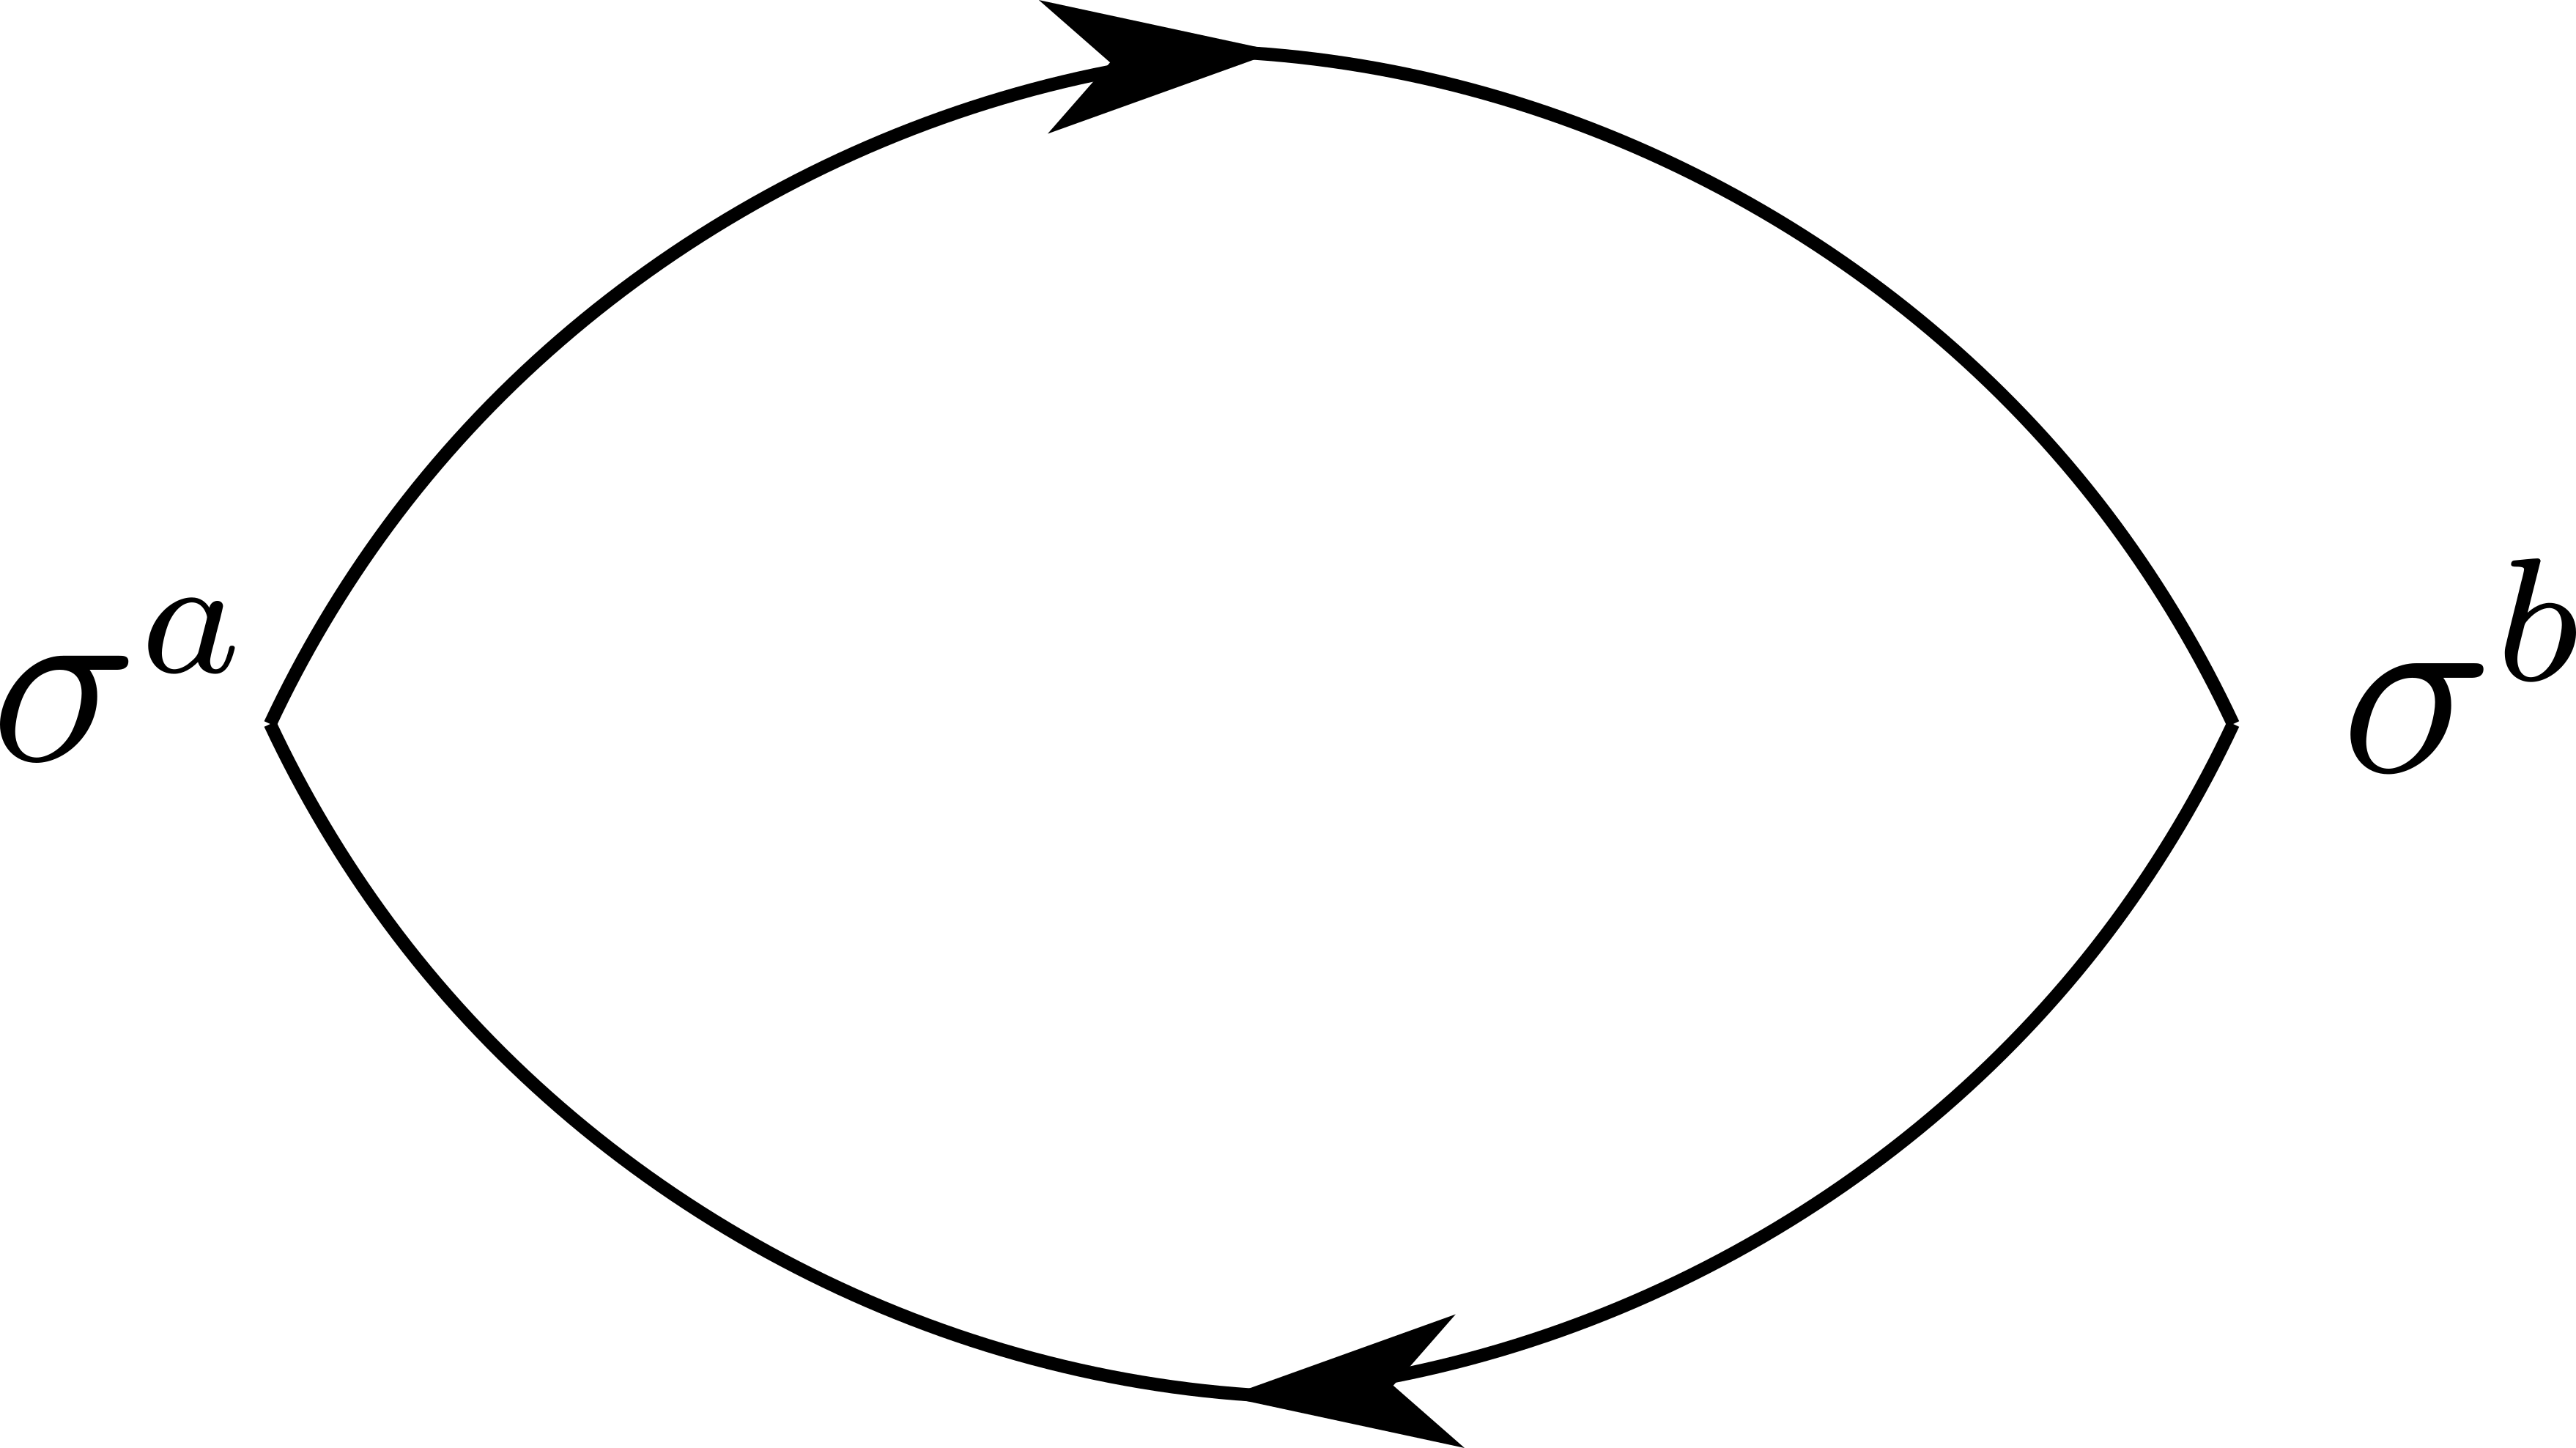
\includegraphics[scale=0.3]{poppov1.png} 
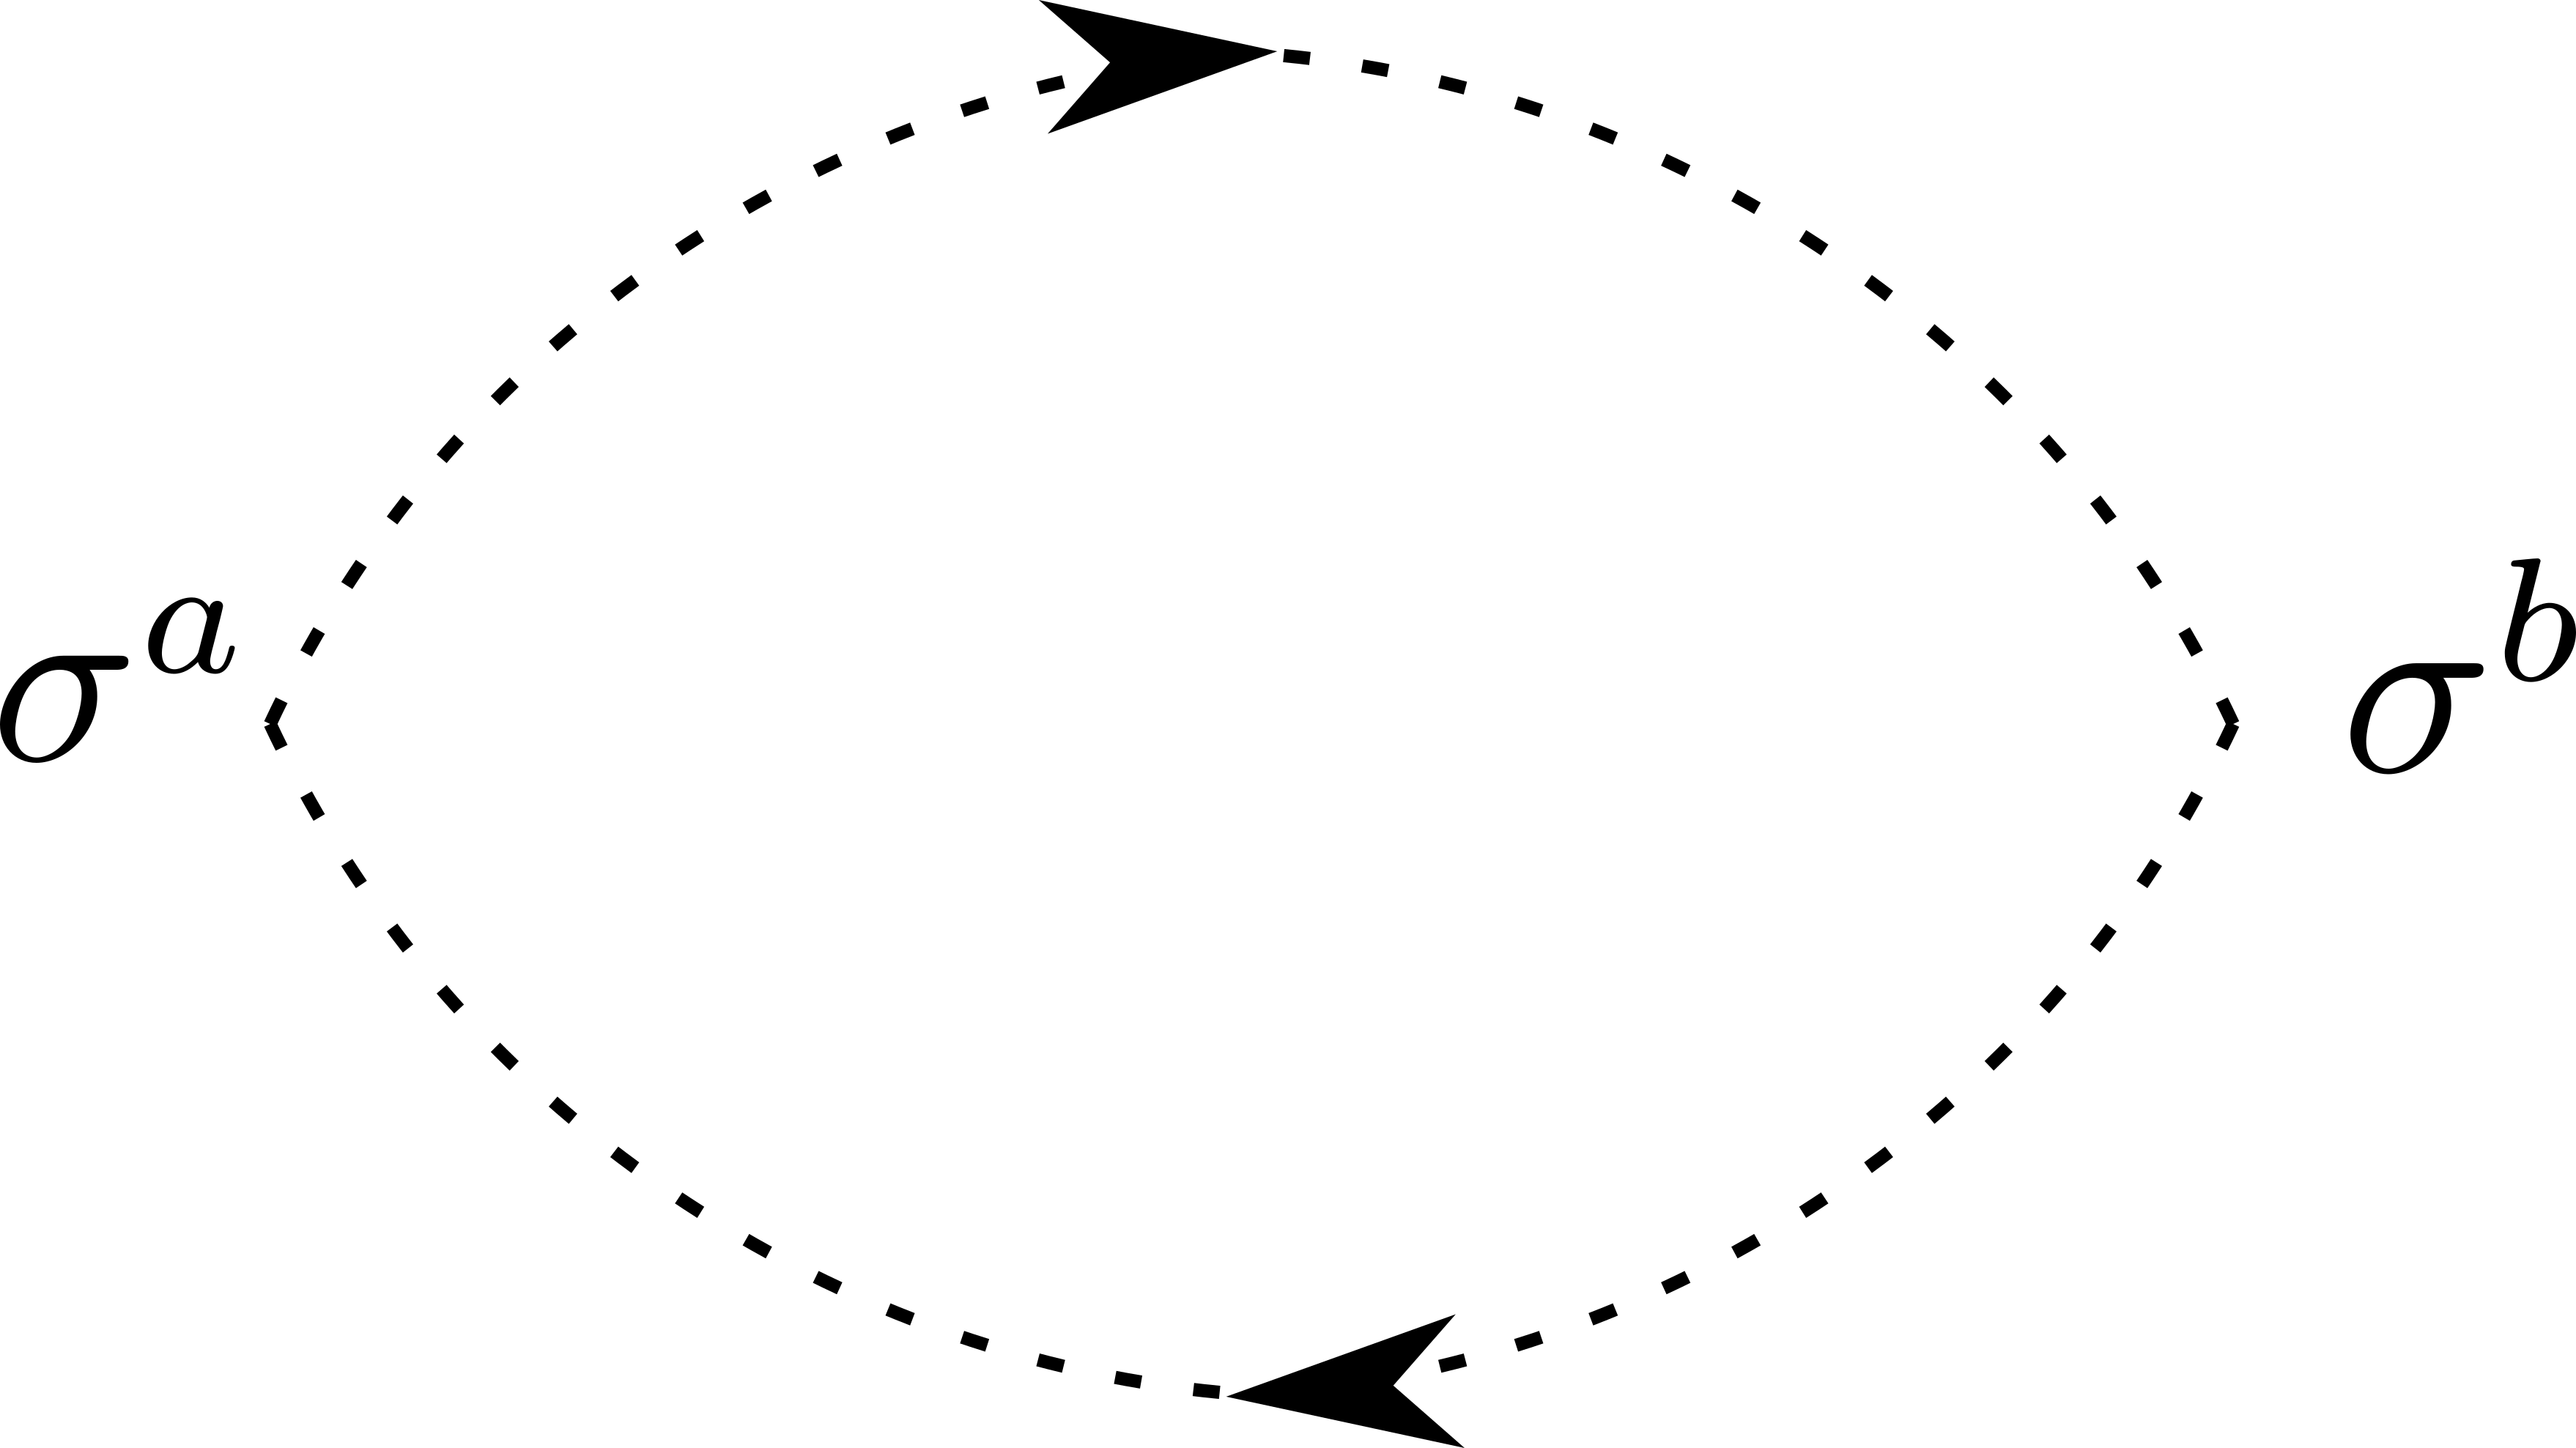
\includegraphics[scale=0.3]{poppov2.png}
\end{figure}\\\\
The dotted lines are the impurity Greens function, so that diagram gives the impurity contribution to the susceptibility.
Similarly, the solid lines are the conduction electron Greens function.
The first diagram gives
\beq
\chi_c = -k_B T \sum_{k,\omega_n,\phi_0} \bra{\phi_0} \sigma^a G(k,i\omega_n)\sigma^bG_k(i\omega_n)\ket{\phi_0}
\eeq
The sum over the ground states \il{\ket{\phi_0}} constitutes a trace, so we can write it as
\beq
\chi_c &= -k_B T \sum_{k,\omega_n} \text{Tr}\qq{\sigma^a G(k,i\omega_n)\sigma^bG(k,i\omega_n)} \\
       &= -2 k_B T \sum_{k,\omega_n} G^2(k,i\omega_n)\\
       &= -2 k_B T \sum_{k,\omega_n} \rr{i\omega_n - \epsilon_k}^{-2}\\
       &= 2 \sum_k \dv{}{\epsilon_k}k_B T\sum_{\omega_n} \rr{i\omega_n - \epsilon_k}^{-1}
\eeq
Now, it can be shown that
\beq
k_B T\sum_{\omega_n} \rr{i\omega_n - \epsilon_k}^{-1} = f(\epsilon_k) - \hf
\eeq
where \il{f(\epsilon_k)} is the FD-distribution at \il{\epsilon_k}.
Therefore,
\beq
\chi_c &=2 \sum_k \dv{f(\epsilon_k)}{\epsilon_k}= 2\sum_k \rho(\epsilon_k) = 2 N(0)
\eeq
The second diagram gives
\beq
\chi_d^{(0)} = -k_B T \sum_{\omega_n} \text{Tr}\qq{\sigma^a G_d(i\omega_n)\sigma^bG_d(i\omega_n)} \\
\eeq
In the Popov-Fedotov scheme, we replace the impurity Greens function with
\beq
G_d = \frac{1}{i\omega_n - \lambda_d}
\eeq
where \il{\lambda_d = i\pi\fr{1}{2\beta}} is the imaginary chemical potential introduced.
Since this is, for mathematical purposes, the same as the conduction Greens function with \il{\lambda_d} replacing \il{\epsilon_k}, we again get
\beq
\chi^{(0)}_d &=2 \dv{f(\lambda_d)}{\lambda_d}= -2\beta\fr{e^{\beta \lambda_d}}{\rr{1+e^{\beta \lambda_d}}^2} = \beta
\eeq
The first order diagrams are
%\begin{center} 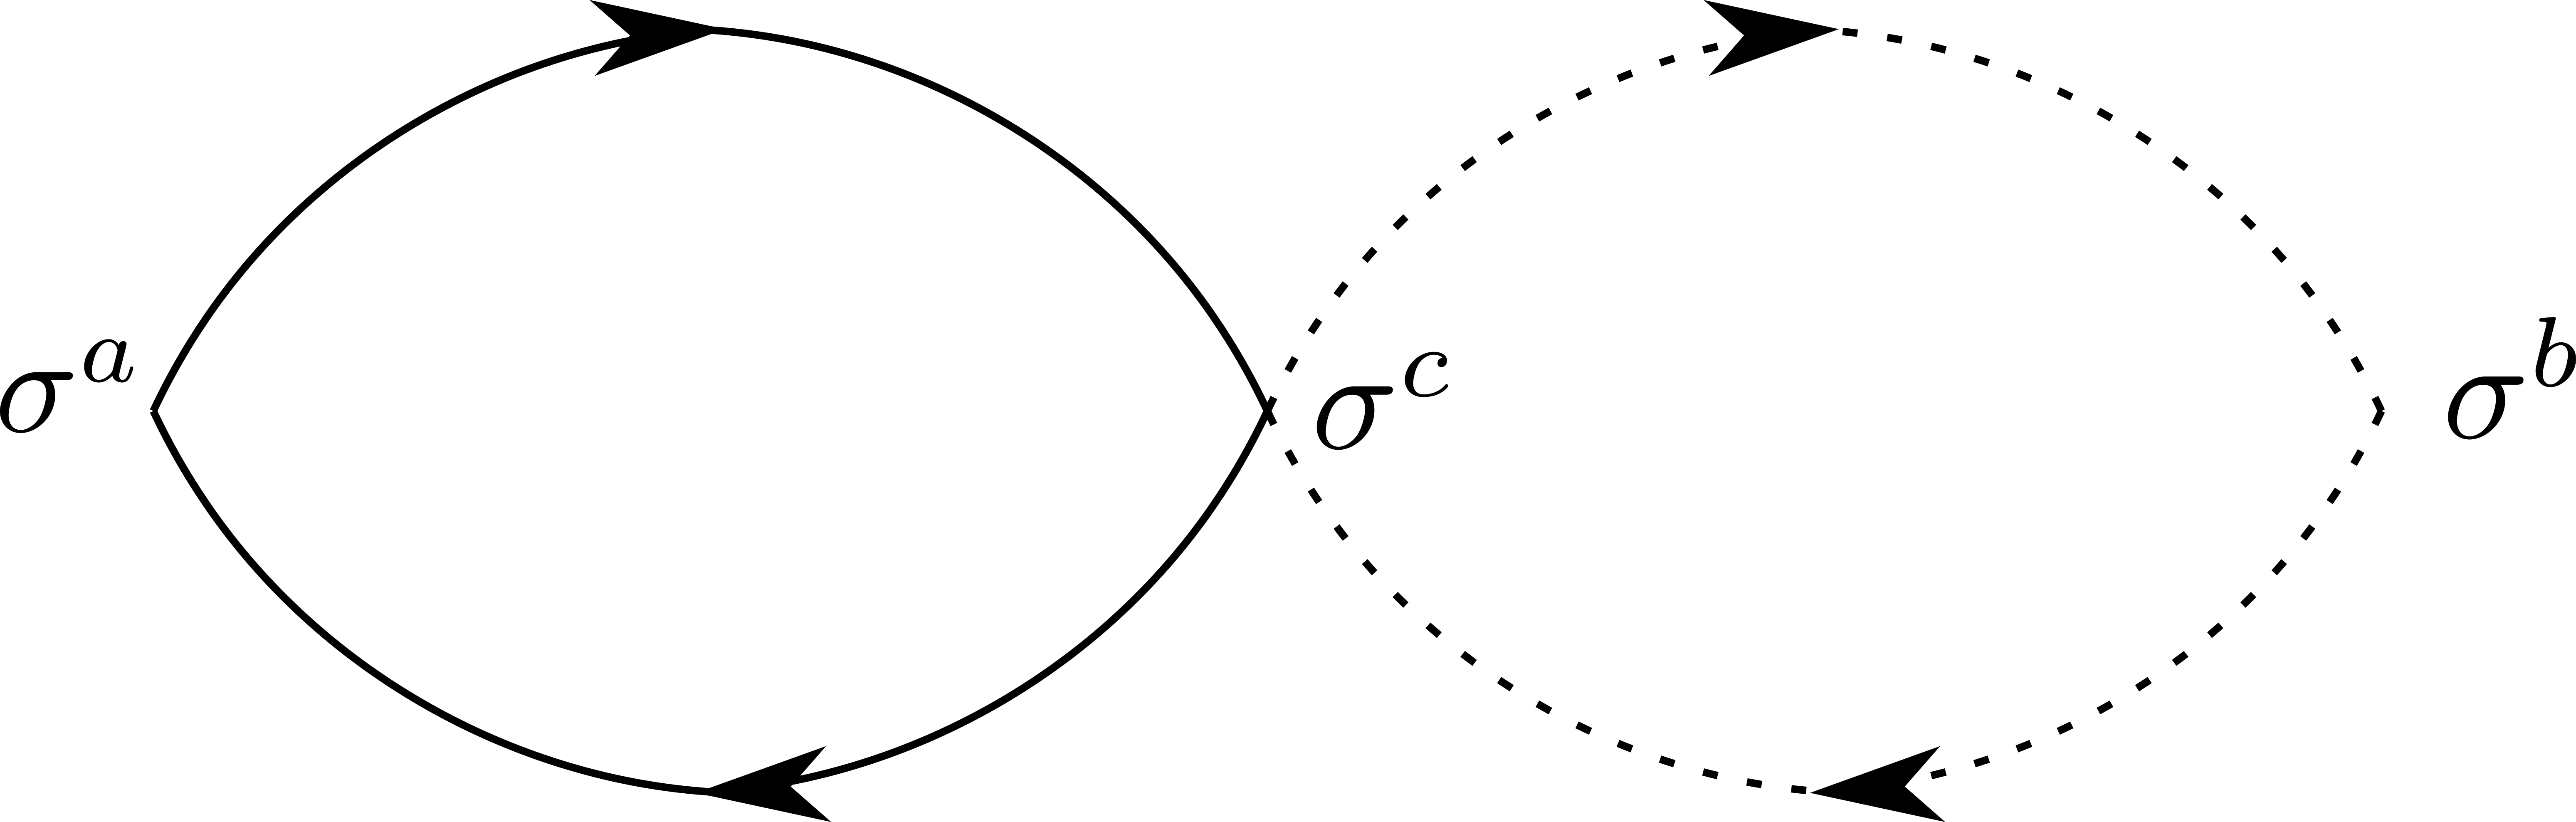
\includegraphics[scale=0.3]{poppov3.png} \end{center}
%\begin{center} 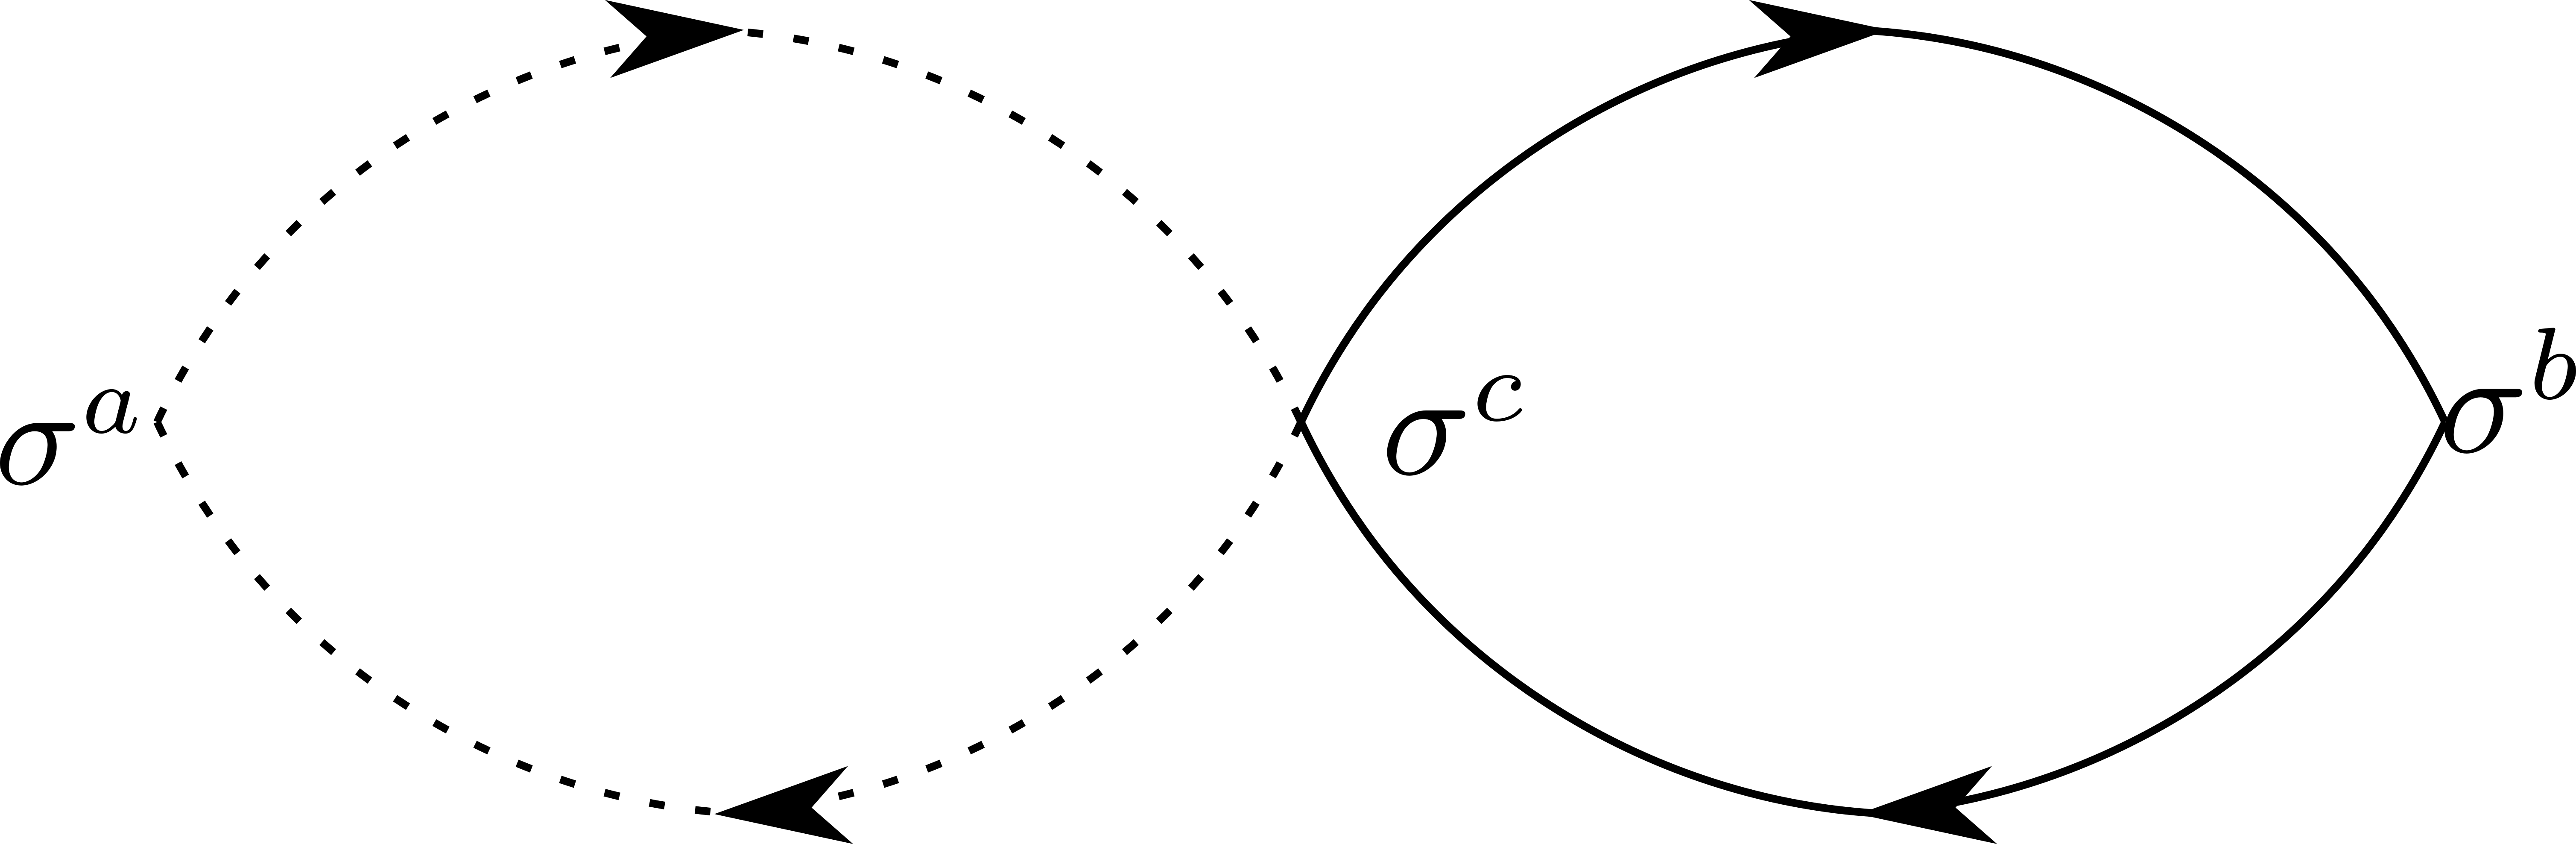
\includegraphics[scale=0.3]{poppov4.png} \end{center}
The first diagram gives
\beq
\chi^{(1)} = \chi_c \rr{-\fr{J}{2}} \chi_d = -\beta JN(0)
\eeq
The second one gives
\beq
\chi_d^{(1)} = \chi_d \rr{-\fr{J}{2}} \chi_c = -\beta JN(0)
\eeq
The total susceptibility is
\beq
\chi_d = \chi^{(0)}_d + \chi_d^{(1)} = \beta\rr{1 - 2 J N(0)}
\eeq
\subsection{Nozières' local Fermi liquid theory}
Wilson's numerical renormalization group calculation showed that the low temperature specific heat contribution from the singlet is linear in temperature
\beq
C_V = \gamma T
\eeq
This suggests that the strong-coupling limit of the Kondo model is a Fermi liquid.\\
The singlet state (\il{s=0}) has an energy
\beq
E_g = J\qq{2\vec S_e \cdot \vec S_d} = J\qq{S^2 - S_d^2 - S_e^2} = J\qq{s\rr{s+1} - \fr{3}{2}} = -\fr{3J}{2}
\eeq
Since the interaction term is spherically symmetric, it suffices to consider a one dimensional chain of conduction electrons with the impurity site coupling to the conduction electron at the origin.
This electron forms a singlet with the impurity electron,
\beq
\fr{\ket{0_\ua,d\da} - \ket{0_\da,d_\ua}}{\sqrt 2}
\eeq
Considering a tight-binding model, the only electron that can hop to the zeroth site is the one on the first site.
The hopping of this electron on to the zeroth site would lead to an energy of
\beq
E_1 = -\fr{3}{2}J + \fr{3}{2}J = 0
\eeq
because the new electron would have the spin opposite to the other electron on the \il{0^\text{th}} site.
This means that breaking the singlet raises the energy by \il{\fr{3}{2}J}.
At low temperatures and very large \il{J}, this is not possible.
That being said, there can always be virtual fluctuations into excited states.
For example, the impurity electron can tunnel into the conduction band (\il{n_d = 0}) or another conduction electron may scatter into the impurity site (\il{n_d = 2}).
Both these states have zero energy.
With further virtual excitations, it is also possible to go into the triplet state with energy \il{\fr{J}{2}}.
What this means is that although the singlet is stable with respect to energy-conserving transitions, the singlet is virtually polarizable, with the help of the site 1 electron.
This induces an interaction on the site 1.
Since the interaction on the site 1 is just a manifestation of the polarizability of the singlet, we can either take the singlet with its polarizability and assume the conduction band to be non-interacting, or we can assume the singlet to be static and take the Fermi sea to have a localised interaction at the site 1.
In the latter picture, we have a frozen singlet (which can be ignored) and an interacting Fermi sea.\\\\
The goal \cite{nozieres} is to calculate the change in phase shift suffered by the conduction electrons in the presence of interactions.
In the absence of interactions, the scattered wavefunction is
\beq[shift]
\psi \sim \fr{\sin\qq{kr + \delta(E_k)}}{r}
\eeq
That is, the phase shift is only a function of the energy.
At the Fermi surface, this value \il{\delta(0)} is \il{\fr{\pi}{2}}, as known from the Friedel sum rule.
\beq
n = \sum_\sigma \fr{\delta}{\pi} \implies 1 = \fr{2\delta}{\pi} \implies \delta = \fr{\pi}{2}
\eeq
\il{n} is the number of conduction electrons bound in the resonance and the sum is over the possible quantum numbers (spin in this case).
\il{\delta(0)} can also be obtained directly from eq.~\ref{shift}, by substituting \il{k=k_F} and noting that the isolation of the 0\uu{th} site means all wavefunctions should shift by \il{\Delta r = a}:
\beq
k_F a = \delta(0) \implies \delta(0) = \fr{\pi}{2a} 2 = \fr{\pi}{2}
\eeq
where the formula for \il{k_F} was used.\\\\
In a Fermi gas, the energy levels are separated by
\beq
\Delta \epsilon = \pd{\epsilon}{k}\Delta k
\eeq
With the condition that the wavefunction should vanish at the boundary, we have \il{\Delta k = k_n - k_{n-1} = \fr{\pi}{L}}.
Hence,
\beq
\Delta \epsilon = \pd{\epsilon}{k}\fr{\pi}{L}
\eeq
However, this changes in the presence of the impurity.
Because of eq.~\ref{shift}, the boundary condition becomes
\beq
k_nL + \delta(\epsilon_k) = n\pi \implies k_n = \fr{n\pi}{L} - \fr{\delta}{L} = k_n^0 -\fr{\delta(\epsilon_k)}{L}
\eeq
The energy becomes
\beq
\epsilon(k) &= \epsilon(k^0) + \pd{\epsilon}{k}\rr{k - k_0}\\
	    &= \epsilon_k - \pd{\epsilon}{k}\fr{\delta(\epsilon_k)}{L}
\eeq
In the Landau formulation of an interacting Fermi liquid, the phase shifts will depend on the quasiparticle occupation probabilities \il{n_{k\sigma}}.
Hence,
\beq
\wl \epsilon_\sigma(k) = \epsilon_k - \pd{\epsilon}{k}\fr{\delta_\sigma(\epsilon_k,\{n_{q,\sigma}\})}{L}
\eeq
In bulk Fermi liquid, we expand the quasiparticle energy in the deviation of the quasiparticle distribution \il{n_k} from the ideal Fermi-Dirac distribution \il{n^0_k},
\beq[fliq]
\wl \epsilon_p = \underbrace{\epsilon_F}_{\text{Fermi gas}} &+ \overbrace{\fr{p_F^*}{m}\rr{p-p_F}}^{\text{linear contribution for \it{p} close to }p_F} \\
	    &+ \underbrace{\sum_{q\sigma}f(p,q)\rr{n_q - n^0_q}}_{\text{interacting between two quasiparticles at momenta \it{p} and \it{q}}}
\eeq
Similarly, for this local Fermi liquid, the phase shift depends on the energy of the quasiparticle \il{\wl \epsilon} and the quasiparticle occupation \il{n_{q\sigma}}.
Accordingly,
\beq
\delta_\sigma(\wl \epsilon,\{n_{q,\sigma}\}) = \delta_\sigma(\wl \epsilon = \epsilon_F, n_k = n^0_k) + \alpha\rr{\wl \epsilon - \epsilon_F} + \Phi \sum_{q\sigma^\prime}\rr{n_{q\sigma^\prime} - n^0_{q\sigma^\prime}}
\eeq
This is just a Taylor expansion of \il{\delta_\sigma} around \il{\tilde \epsilon = \epsilon_F} and \il{n_q = n^0_q}.
\il{\Phi} and \il{\alpha} play the same role as \il{f} and \il{\fr{p_F^*}{m}} in eq.~\ref{fliq}.
Specifically, \il{\Phi} represents the onsite interaction between quasiparticles of  opposite spin and 
\beq
\alpha = \dv{\delta_\sigma}{E}
\eeq
Since \il{\Phi} acts only between quasiparticles of opposite spin, the last term can be simplified by requiring \il{\sigma^\prime = -\sigma},

\beq[phases]
\delta_\sigma(\wl \epsilon,\{n_{q,\sigma}\}) = \delta_\sigma(\wl \epsilon = \epsilon_F, n_k = n^0_k) + \alpha\rr{\wl \epsilon - \epsilon_F} + \Phi \sum_{q}\delta n_{q,-\sigma}
\eeq
Since the singlet is isolated from the Fermi liquid, any change in the chemical potential will not affect the average occupation of the impurity site \il{\avg{n_d}}, and since we know that \il{\avg{n_d} = \fr{2\delta(0)}{\pi}}, this means that \il{\delta(0)}, the phase shift at the Fermi surface, is invariant under a change of the chemical potential.
This in turn means that the resonance scattering (\il{\delta = \fr{\pi}{2}}) will always be pinned to the Fermi surface.
With this knowledge, let us explicitly try to calculate the change in the phase shift at Fermi surface when we change the chemical potential by \il{\Delta \mu}.
Before the change in chemical potential,
\beq
\delta^0_\ua = \fr{\pi}{2} + \Phi\sum_q \delta n^0_{q\da}
\eeq
Since \il{\delta n^0 = n^0 - n^0 =0},
\beq
\delta^0_\ua = \fr{\pi}{2}
\eeq
After the change in chemical potential, \il{\epsilon_F^\prime = \epsilon_F + \Delta \mu} and 
\begin{gather}
N(\mu = 0) = N^0 \\
N(E^\prime = E+\mu) = N(E^\prime = E) + \dv{N}{E^\prime}\rr{E^\prime - E} = N^0 + \rho \Delta \mu\\
\implies \sum_q \delta n_q = N - N^0 = \rho \Delta \mu
\end{gather}
Hence, from eq.~\ref{phases},
\beq
\delta_\ua &= \fr{\pi}{2} + \alpha\rr{\epsilon_F^\prime - \epsilon_F} + \Phi\sum_q \delta n_{q\da}\\
	   &= \delta^0_\ua + \alpha\Delta\mu + \Phi \rho \Delta \mu
\eeq
Hence the change in the phase is
\beq
0 = \Delta \delta_\ua = \Delta \mu\rr{\alpha + \Phi \rho} \implies \alpha = -\Phi\rho
\eeq\\\\
This shows that the interaction term \il{\Phi} is responsible for pinning the resonance at the Fermi level; without that term in the formalism, the occupancy of the impurity site will change.
This is similar to the fact that the interaction term \il{f(k,k^\prime)} in the bulk Fermi liquid is responsible for making the Landau theory invariant under Galilean transformations.\\\\
Now we can calculate the density of states.
From the boundary condition, we have
\beq
n_\sigma = \fr{kL}{\pi} + \fr{\delta_\sigma(E)}{\pi} = n^0 + \fr{\delta_\sigma(E)}{\pi}
\eeq
Hence,
\beq
\rho &= \dv{n_\sigma}{E} = \rho^0 + \fr{1}{\pi}\dv{\delta_\sigma}{E} \\
\implies \rho&=\rho^0 + \fr{1}{\pi}\alpha
\eeq
\il{\rho^0} is the density of states in absence of the impurity.
The low temperature specific heat of an ideal Fermi liquid can be shown to be
\beq
C_v^0 = \gamma T = \fr{\pi^2 k_B^2}{3} \mathcal{N}(0) T
\eeq
The interacting Fermi liquid is just a renormalised version of the Fermi gas, with a modified density of states \il{\fr{1}{\pi}\alpha}.
Hence, the impurity contribution to the specific heat is
\beq
C_v &= \fr{\pi^2 k_B^2}{3}\rr{\rho_\ua + \rho_\da} T\\
    &=\fr{2\alpha}{\pi} \fr{\pi^2 k_B^2}{3} T
\eeq
In presence of a magnetic field \il{B}, the magnetization is 
\beq
m = \delta n \times \mu
\eeq
where \il{\mu} is the magnetic moment
\beq
\mu = -\fr{g}{2}\mu_B 
\eeq
and \il{\delta n} is the difference in number between up and down electrons
\beq
\delta n = \avg{n_\ua} - \avg{n_\da} = \fr{1}{\pi}\rr{\delta_\ua - \delta_\da}
\eeq
In the presence of the magnetic field, all energies get modified,
\beq
E^B_\sigma = E - \sigma \fr{g\mu_B}{2}B
\eeq
Hence,
\beq
\sum_k \delta n_{k\sigma} = N_\sigma(E^B_\sigma) - N(E) = \dv{N}{E^B}\rr{E^B - E} = -\rho \fr{g \mu_B}{2}\sigma B
\eeq
This modifies the phase shift at the Fermi surface,
\beq
\delta_\sigma(\epsilon_F) &= \fr{\pi}{2} + \alpha\rr{\epsilon_F - \fr{g \mu_B}{2}\sigma B - \epsilon_F} + \Phi\sum_q \delta n_{q,-\sigma}\\
			  &= \fr{\pi}{2} - \sigma \fr{g \mu_B}{2}\alpha B + \Phi \rho \fr{g \mu_B}{2}\sigma B\\
			  &= \fr{\pi}{2} - 2\alpha\fr{g \mu_B}{2}\sigma B
\eeq
Hence,
\beq
\delta n = \fr{1}{\pi}\rr{\delta_\ua - \delta_\da} = -\fr{4\alpha B}{\pi}\fr{g \mu_B}{2}
\eeq
The susceptibility is
\beq
\chi = \pd{m}{B} = \pd{}{B}\mu\delta n = \fr{4\alpha}{\pi}\rr{\fr{g \mu_B}{2}}^2
\eeq

The susceptibility for an ideal Fermi gas can be calculated similarly.
The additional energy of an electron with spin \il{\sigma} in a magnetic field \il{B} is \il{-\sigma \fr{g}{2}\mu_B B}.
The magnetization induced at the Fermi surface is \il{\delta n \times \mu}, where \il{\mu} is the magnetic moment
\beq
\mu = -\fr{g}{2}\mu_B 
\eeq
and \il{\delta n} is the difference in number between up and down electrons
\beq
\delta n = n_\ua(0) - n_\da(0) = n_\ua(\epsilon_F - \fr{g}{2}\mu_B B) - n_\da(\epsilon_F + \fr{g}{2}\mu_B B) = -\hf\mathcal{N}(0)gB \mu_B
\eeq
\il{\mathcal{N}(0) = \pd{n}{E}\bigg |_{\epsilon_F}} is the density of states at the Fermi energy and the \il{\hf} is because we are counting electrons of a particular spin only.
Therefore,
\beq
m = \delta n \times \mu = \mathcal{N}(0)\rr{\fr{g}{2} \mu_B}^2B
\eeq
The magnetic susceptibility comes out to be 
\beq
\chi^0 = \pd{m}{B}\bigg |_{B \ra 0} = \mathcal{N}(0)\rr{\fr{g}{2} \mu_B}^2
\eeq
The Wilson ratio \il{R} can now be computed,
\beq
R = \frac{\chi/\chi_0}{C_v/C_v^0} = \frac{4\alpha/\pi\mathcal{N}(0)}{2\alpha/\pi\mathcal{N}(0)} = 2
\eeq

\subsection{Numerical renormalization group calculation}
Wilson's idea \cite{wilson} was to remove the limitations of the perturbative nature of Anderson's scaling method.
To that end, we transformed the Hamiltonian into a one-dimensional chain, and then iteratively diagonalised chains of increasing length.
The Hamiltonian we are working with is
\beq
H = \sum_k \epsilon_k n_k + J \vec S_d \cdot \vec \sigma_e
\eeq
where \il{\vec \sigma_e = \sum_{k_1,k_2,\alpha\beta}c^\dagger_{k_1\alpha}\vec \sigma_{\alpha\beta}c_{k_2,\beta}} is the conduction electron spin at the origin.
This assumes that the exchange interaction \il{J(k,k^\prime} is independent of spin.
To form the linear chain, we construct a new basis in which to express the conduction electron part \il{H_c}, out of the states \il{\ket{0},H_c\ket{0},H_c^2\ket{0},...}.
\il{\ket{0}} is the origin site, where the impurity resides.
The first member of the new basis is \il{\ket{0}}.
The next member is taken to be some state in the subspace of \il{\ket{0}} and \il{H_c\ket{0}},
\beq
\ket{1} = \rr{\lambda_1 H_c\ket{0} + \lambda_2\ket{0}}
\eeq
This is a general form for any ket in the subspace spanned by \il{\ket{0}} and \il{H_c\ket{0}}.
Since we want the state to be normalised , we can shift one of the parameters to the denominator:
\beq
\ket{1} = \fr{1}{\gamma_0}\rr{H_c\ket{0} + \lambda\ket{0}}
\eeq
where \il{\gamma_0} sets \il{\avg{1|1} = 1}.
The remaining parameter is set by requiring \il{\avg{1|0} = 0}.
That gives
\beq
\lambda = -\avg{0|H_c|0}
\eeq
Therefore,
\beq
\ket{1} = \fr{1}{\gamma_0}\rr{H_c\ket{0} -\avg{0|H_c|0}\ket{0}}
\eeq
The general state can be shown to be
\beq[chain]
\ket{n+1} = \fr{1}{\gamma_n}\rr{H_c \ket{n} - \ket{n}\avg{n|H_c|n-1}-\ket{n-1}\avg{n-1|H_c|n}}
\eeq
From eq.~\ref{chain}, by multiplying \il{\bra{n^\prime}} from left, we get
\beq
\delta_{n^\prime,n+1} = \fr{1}{\gamma_n}\qq{\rr{H_c}_{n^\prime,n} + \rr{H_c}_{n,n-1}\delta_{n^\prime,n} + \rr{H_c}_{n-1,n}\delta_{n^\prime,n-1}}
\eeq
Clearly, for \il{n^\prime < n-1} or \il{n^\prime > n+1}, we get
\beq
\rr{H_c}_{n^\prime,n} = 0
\eeq
so the only non-zero terms are for \il{n^\prime = n-1,n,n+1}.
For \il{n^\prime = n+1} gives
\beq
\rr{H_c}_{n+1,n} = \gamma_n
\eeq
Taking the complex conjugate of this gives
\beq
\gamma_n^* = \rr{H_c^\dagger}_{n,n+1} = \rr{H_c}_{n,n+1}
\eeq
Defining 
\beq
\rr{H_c}_{n,n} = \epsilon_n
\eeq
we can write
\beq
H_c &= \sum_{n_1,n_2} \ket{n_1}\bra{n_1} H_c \ket{n_2}\bra{n_2}\\
    &= \sum_{n}\epsilon_n \ket{n}\bra{n} + \sum_{n}\rr{\gamma_n\ket{n} \bra{n+1}+ \gamma^*_n\ket{n+1} \bra{n}}\\
    &= \sum_{n}\epsilon_n \hat n_n + \sum_{n}\rr{\gamma_nc^\dagger_n c_{n+1}+ \gamma^*_nc^\dagger_{n+1} c_{n}}
\eeq
The diagonalization of these chains become impossible for \il{n>8}.
To remedy this problem, Wilson, after diagonalization a chain of a particular length, retained only the lowest parts of the spectrum, and the Hamiltonian for the next stage was formed out of these low-lying states.
This keeps the size of the Hilber space (and hence the matrices) manageable.
Another problem is that as one goes on adding sites to the chain, the couplings need to die off, otherwise this process will never converge.

\subsubsection{Logarithmic discretization}
First, note that up to first order
\beq
\epsilon_k = \epsilon_F + (k-k_F)\pd{\epsilon_k}{k}
\eeq
By choosing \il{k_F = \epsilon_F = 0}, we get \il{\epsilon_k = k}.\\\\
Wilson divided the conduction band into patches, \il{[\Lambda^{-(n+1)},\Lambda^{-n}]}, for \il{n=1,2,3..}.
The width of each interval is
\beq
d_n = \Lambda^{-n}\rr{1-\Lambda^{-1}}
\eeq
We can now define orthogonal functions in this \il{n^\text{th}} interval \il{k \in [\Lambda^{-(n+1)},\Lambda^{-n}]},
\beq
\psi_{m,n}(k) = \fr{1}{\sqrt{d_n}} \ex{\fr{2\pi i m}{d_n} k}
\eeq
They allows us to define a new set of creation operators,
\beq
a^\dagger_{m,n} = \sum_k \psi_m(k)c^\dagger_k
\eeq
Similarly functions can be defined in the negative interval \il{-k \in[\Lambda^{-(n+1)},\Lambda^{-n}]}.
\begin{gather}
	\phi_{m,n}(k) = \fr{1}{\sqrt{d_n}} \ex{-\fr{2\pi i m}{d_n} k}\\
	b^\dagger_{m,n} = \sum_k \phi_m(k)c^\dagger_k
\end{gather}
Then,
\beq
a^\dagger_{m,n} + b^\dagger_{m,n} = \fr{2}{\sqrt{d_n}}\sum_{\pm k \in []} \cos \rr{\fr{2\pi mk}{d_n}} c^\dagger_k
\eeq
Summing over \il{n} involves summing over all momenta.
\beq[zerom]
\sum_n \rr{a^\dagger_{m,n} + b^\dagger_{m,n}} &= \fr{2}{\sqrt{d_n}}\sum_{k} \cos \rr{\fr{2\pi mk}{d_n}} c^\dagger_k\\
\implies \sum_n \rr{a^\dagger_{0,n} + b^\dagger_{0,n}} &= \fr{2}{\sqrt{d_n}}\sum_{k} c^\dagger_k\\
\eeq
For the momentum-independent \il{J(k,k^\prime)}, the coupling term involves.
\beq
\sum_{k,q}c^\dagger_k c_q = \sum_{k}c^\dagger_k \sum_{q}c_q
\eeq
Looking at eq.~\ref{zerom}, we see that the impurity spin is coupled only to the \il{m=0} operators.
This is where the approximation comes in, in Wilson's scheme.
All the \il{m} values other than \il{m=0} are ignored.\\\\
Wilson chose
\beq
\epsilon_n = 0, \gamma = D^\prime \Lambda^\fr{-n}{2}
\eeq
with \il{\Lambda>1}.
The Hamiltonian for \il{N} sites then turns out to be
\beq[run]
H_N = D^\prime \sum_{n=0}^{N-1} \Lambda^{-\fr{n}{2}}\rr{c^\dagger_n c_{n+1}+c^\dagger_{n+1} c_{n}} + 2 J \vec S_d \cdot \vec S_e
\eeq
The next step involves adding another site to the chain.
The next Hamiltonian is hence
\beq
H_{N+1} = H_N + D^\prime \Lambda^{-\fr{N}{2}}\rr{c^\dagger_N c_{N+1}+c^\dagger_{N+1} c_{N}}
\eeq
To compare the couplings, and hence the Hamiltonians, at each value of \il{N}, we need to rescale the Hamiltonians \il{H_N} so that the lowest energy scale is independent of the running index \il{N}.
Looking at eq.~\ref{run}, the lowest energy scale is \il{\Gamma_N = D^\prime \Lambda^{-\fr{N-1}{2}}}.
Hence, the rescaled Hamiltonian is
\beq
\ol H_N = \frac{H_N}{\Gamma_N} = \fr{\Lambda^{\fr{N-1}{2}}}{D^\prime} H_N
\eeq
The utility can be seen by noting the relation between \il{\ol H_{N+1}} and \il{\ol H_N},
\beq[rec]
\ol H_{N+1} &= \fr{\Lambda^{\fr{N}{2}}}{D^\prime}\qq{H_N + \Lambda^{\fr{-N}{2}}D^\prime\rr{c^\dagger_N c_{N+1}+c^\dagger_{N+1} c_{N}}}\\
\implies \ol H_{N+1} &= \Lambda^\hf\ol H_N + \rr{c^\dagger_N c_{N+1}+c^\dagger_{N+1} c_{N}}
\eeq
In the series of Hamiltonians \il{\{H_N\}}, the couplings to the extra site are all same, so the lowest energy scales are all of the same order.
This allows us to construct a flow of the Hamiltonians.
The real Hamiltonian is the unscaled one, so it is given by
\beq
H = \lim_{N \ra \infty} H_N = \lim_{N \ra \infty} D^\prime \Lambda^\fr{1-N}{2} \ol H_N
\eeq
Since \il{\ol H_N} is exactly diagonalised with a spectrum \il{\{E_m,\ket{m}\}}, it can be written down as
\beq
\ol H_N = \sum_m E_m \ket{m}\bra{m}
\eeq
The next Hamiltonian is then
\beq
\ol H_{N+1} = \Lambda^\hf \sum_m E_m \ket{m}\bra{m} + \sum_{m.m^\prime}\rr{ C(m,m^\prime) \ket{m}\bra{m^\prime} + \text{h.c.}}
\eeq
This is the same equation as eq.~\ref{rec}, with \il{\ol H_N} expressed in its eigenbasis and the creation and annihilation operators also expressed in that basis; the \il{C(m,m^\prime)} are just the matrix elements of \il{c} and \il{c^\dagger} in that basis.\\\\
To check whether the guesses about the fixed points are true, Wilson did the following.
He set \il{J=0.009} and then then calculated the lowest excitations of the Hamiltonians obtained from the NRG in the limit of large \il{N}.
They indeed correspond to the excitations of the Kondo hamiltonian at \il{J = \infty}, meaning that under the application of the NRG, the \il{J=0.009} Hamiltonian flowed to the fixed-point Hamiltonian \il{J = \infty}.

\pagebreak
\subsection{Correspondence between the Kondo model fixed-point and a local Fermi liquid - Topological interpretation of Wilson ratio}
\subsubsection{Local Fermi liquid}
The fixed-point Hamiltonians \cite{hewsonp} are found to represent interacting Fermi liquids.
The effective Hamiltonian can be shown to resemble the Anderson model, but with modified parameters,
\beq
H_\text{eff} = \sum_k \epsilon_k n_k + \sum_k{V_k c^\dagger_d c_k + \text{h.c.}} + U n_{d\ua}n_{d\da}
\eeq
The parameters \il{\epsilon_k,V_k,U} are not the same as the Anderson model we start with, but I am using the same symbols for convenience.
The interaction term \il{U} is the leading irrelevant operator near the low-energy fixed point.
For \il{T \ra 0}, assuming only single excitations, the interacting term will not get invoked.\\\\
Under mean-field,
\beq
n_{d\ua}n_{d\da} &\approx n_{d\ua}\avg{n_{d\da}} + \avg{n_{d\ua}}n_{d\da} - \avg{n_{d\ua}}\avg{n_{d\da}}\\
\implies \avg{n_{d\ua}n_{d\da}} &= \avg{n_{d\ua}}\avg{n_{d\da}}\\
				&= \sum_{k,q}\avg{n_{k\sigma}} \avg{n_{q,-\sigma}}\\
\eeq
where \il{N} is the number of sites.
Note that the number of excitations, \il{\avg{n_q}} has to be defined differently for the states above and below the Fermi surface.
For excited states above \il{\epsilon_F}, the number of excitations is given usually:
\beq
\avg{n_q^>} = \bra{\psi^>}c^\dagger_k c_k\ket{\psi^>} = n^p_k
\eeq
where \il{n^p_k} stands for the number of particles.
For states below \il{\epsilon_F}, however, we need to count the number of holes:
\beq
\avg{n_q^<} = \bra{\psi^<}c^\dagger_k c_k\ket{\psi^<} = -\bra{\psi^<}c_k c^\dagger_k \ket{\psi^<} = -n^h_k
\eeq
where \il{n^h_k} stands for the number of holes.
We can thus define a generalized excitation:
\beq
\avg{\delta n_{k,\sigma}} = \begin{cases} n^p_k, &\epsilon_k > \epsilon_F\\ -n^h_k, &\epsilon_k < \epsilon_F\end{cases}
\eeq
Replacing the quasiparticle excitations with their expectation values, the effective one-particle energy becomes
\beq
\epsilon_{k\sigma} = \epsilon_k + U\sum_q \avg{\delta n_{q,-\sigma}} \equiv \epsilon_k + U\avg{\delta n_{-\sigma}}
\eeq
This is analogous to the Landau quasiparticle energy functional, eq.~\ref{temp_en}, \il{U} acting as the interaction between the quasiparticles.
\il{\delta n > 0} acts as the excitations from the ground state.
\pb
The interacting density of states is
\beq[dosint]
\rho_{d\sigma}(\omega) = \fr{\Delta}{\pi}\fr{1}{\rr{\omega - \epsilon_d^*}^2 + \Delta^2}
\eeq
where \il{\epsilon_d^* = \epsilon_d + U\avg{\delta n_{-\sigma}}}.

\subsubsection{Calculation of \il{C_v}}
To calculate the specific heat, \il{C_v = \dv{\avg{E}}{T}}, note that a change in temperature would modify the quasiparticle distribution \il{\delta n_{k\sigma}} and hence the quasiparticle energies \il{\epsilon_{k\sigma}}.
This leads to a complicated feedback effect.
However, at low temperatures, higher order excitations will be very low and we can approximate by considering only the variation in the distribution:
\beq
\dv{\avg{E}}{T} &= \sum_{k,\sigma}\epsilon_{k\sigma}\dv{\avg{\delta n_{k\sigma}}}{T}\\
\eeq
%\beq
%\dv{\avg{E}}{T} &= \dv{}{T}\sum_{k,\sigma}\epsilon_{k\sigma}\avg{\delta n_{k\sigma}}\\
%		&= \sum_{k,q,\sigma}\dv{}{T}\rr{\epsilon_{k}\avg{\delta n_{k\sigma}} + U\avg{\delta n_{q,-\sigma}}\avg{\delta n_{k\sigma}}}\\
%		&= \sum_{k,q,\sigma}\rr{\epsilon_{k}\dv{\avg{\delta n_{k\sigma}}}{T} + U\dv{\avg{\delta n_{q,-\sigma}}}{T}\avg{\delta n_{k\sigma}} + U\avg{\delta n_{q,-\sigma}}\dv{\avg{\delta n_{k\sigma}}}{T}}\\
%		&=\sum_{k,q,\sigma}\rr{\epsilon_{k}\dv{\avg{\delta n_{k\sigma}}}{T} + 2U\avg{\delta n_{q,-\sigma}}\dv{\avg{\delta n_{k\sigma}}}{T}}\\
%		&=\sum_{k,q,\sigma}\rr{2\epsilon_{k\sigma} - \epsilon_k}\dv{\avg{\delta n_{k\sigma}}}{T}
%\eeq
Since the quasiparticle excitations are adiabatically connected to the free electron excitations, \il{\avg{\delta n_{k\sigma}}} will follow a Fermi-Dirac distribution:
\beq
\avg{\delta n_{k\sigma}}(T) &= \fr{1}{e^{\beta\epsilon_{k\sigma}} + 1}\\
\implies \dv{\avg{\delta n_{k\sigma}}}{T} &= \fr{e^{\beta\epsilon_{k\sigma}}}{\rr{e^{\beta\epsilon_{k\sigma}} + 1}^2}\qq{\fr{1}{k_B T^2}\epsilon_{k\sigma} -\fr{1}{k_B T}\rr{2\epsilon_{k\sigma} - \epsilon_k}\dv{\avg{\delta n_{k\sigma}}}{T}}
\eeq
At sufficiently low temperatures, the first term will dominate over the others (\il{T^{-2} \gg T^{-1}}).
Hence the low temperature specific heat can be written as
\beq
\dv{\avg{E}}{T} &= \sum_{k,\sigma}\epsilon_{k\sigma}\fr{e^{\beta\epsilon_{k\sigma}}}{\rr{e^{\beta\epsilon_{k\sigma}} + 1}^2}\fr{1}{k_B T^2}\epsilon_{k\sigma}\\
		&= \fr{1}{k_B T^2}\sum_{k,\sigma}\epsilon_{k\sigma}^2\fr{e^{\beta\epsilon_{k\sigma}}}{\rr{e^{\beta\epsilon_{k\sigma}} + 1}^2}\\
		&=\fr{1}{k_B T^2}\sum_{\sigma}\int d\epsilon_\sigma \rho(\epsilon_\sigma) \epsilon_{\sigma}^2\fr{e^{\beta\epsilon_{k\sigma}}}{\rr{e^{\beta\epsilon_{k\sigma}} + 1}^2}
\eeq
The function \il{\fr{e^{\beta\epsilon_{k\sigma}}}{\rr{e^{\beta\epsilon_{k\sigma}} + 1}^2}} is very sharply peaked at the Fermi surface \il{\epsilon_\sigma = 0}.
Therefore we can replace the density of states by its value at the Fermi surface.
\beq
\dv{\avg{E}}{T} &=\fr{1}{k_B T^2}\sum_{\sigma}\rho_\sigma(0) \int_{-\infty}^\infty d\epsilon_\sigma\epsilon_{\sigma}^2\fr{e^{\beta\epsilon_{k\sigma}}}{\rr{e^{\beta\epsilon_{k\sigma}} + 1}^2}\\
		&=-\fr{1}{T}\sum_{\sigma}\rho_\sigma(0) \int_{-\infty}^\infty  d\epsilon_\sigma \epsilon_{\sigma}^2f^\prime(\epsilon_\sigma)\\
		&=-\fr{1}{T}\sum_{\sigma}\rho_\sigma(0) \int_1^0 df \epsilon_{\sigma}^2
\eeq
\il{f(\epsilon_\sigma)} is the Fermi-Dirac distribution.
Note that
\beq
\epsilon = k_B T\ln \rr{f^{-1} - 1}\implies \epsilon^2 =k_B^2 T^2\qq{\ln \rr{f^{-1} - 1}}^2
\eeq
Therefore,
\beq
\dv{\avg{E}}{T} &=-k_B^2 T\sum_{\sigma}\rho_\sigma(0) \int_1^0 df \qq{\ln \rr{f^{-1} - 1}}^2
\eeq
The remaining integral gives \il{-\fr{\pi^2}{3}}.
For \il{T \ra 0}, quasiparticle excitations will be absent and we can write \il{\rho_\ua = \rho_\da = \rho_d}:
\beq
\dv{\avg{E}}{T} &=k_B^2 T\sum_{\sigma}\rho_d(0) \fr{\pi^2}{3}\\
		&=2k_B^2 T\rho_d(0) \fr{\pi^2}{3}\\
		&= \gamma_\text{imp}T
\eeq
where
\beq
\gamma_\text{imp} \equiv \fr{C_v}{T} = \fr{2\pi^2}{3}k_B^2\rho_d(0) 
\eeq
This is identical in structure to the Fermi gas result \il{C_v^{(0)} \equiv \gamma^{(0)} T = \fr{2\pi^2}{3}k_B^2\rho^{(0)}_d(0) T}:
\beq
\fr{\gamma_\text{imp}}{\gamma^{(0)}} = \fr{\rho_d(0)}{\rho^{(0)}_d(0)}
\eeq
\subsubsection{Calculation of \il{\chi}}
Under a magnetic field \il{B}, \il{ \epsilon_{k\sigma} \ra \epsilon_{k\sigma} + \sigma h}.
where \il{h=\hf g B \mu_B}.
The magnetisation is
\beq
m &= \fr{g\mu_B}{2}\rr{\delta n_\ua - \delta n_\da}\\
  &=\fr{g\mu_B}{2}\sum_\sigma \sigma\delta n_\sigma\\
  &=\fr{g\mu_B}{2}\sum_{k\sigma} \sigma\pd{n_\sigma}{\epsilon_{k\sigma}}\delta \epsilon_{k\sigma}\\
  &= \fr{g\mu_B}{2}\sum_{k\sigma} \sigma\rho_{k\sigma}\rr{\sigma h + U\delta n_{- \sigma}}\\
  &= \fr{g\mu_B}{2}\sum_{\sigma} \sigma\rho_{\sigma}\rr{\sigma h + U\delta n_{- \sigma}}
\eeq   
On applying the magnetic field, the Fermi energy of spin \il{-\sigma} decreases as \il{\epsilon_F -\sigma h}.
Hence, more number of spin \il{-\sigma} electrons will get excited, the number of such excitations being
\beq
\delta n_{- \sigma} = \sum_q \delta n_{q,-\sigma} = \sum_q \Delta \epsilon_F \rho_{q-\sigma} = \sigma h\rho_{-\sigma}(0)
\eeq
In the last step, I used the fact that the density of states is non-zero only very close to the Fermi surface.
Substituting this in the magnetization gives
\beq
m &= \fr{g\mu_B}{2}h\sum_{\sigma} \sigma^2 \rho_{\sigma}(0)\rr{1 + U\rho_{-\sigma}(0)}\\
  &= \rr{\fr{g\mu_B}{2}}^2 B \sum_{\sigma} \rho_{\sigma}(0)\qq{1 + U\rho_{-\sigma}(0)
}
\eeq
The susceptibility is
\beq[mimp]
\chi_\text{imp} &= \lim_{h \to 0} \pd{m}{B}\\
		&= \rr{\fr{g\mu_B}{2}}^2 \rho_{d}(0)\qq{1 + U\rho_{d}(0)}\sum_{\sigma} \\
		&=\fr{\rr{g\mu_B}^2}{2} \rho_{d}(0)\qq{1 + U\rho_{d}(0)}\\
		&= \chi^{(0)}\fr{\rho_{d}(0)}{\rho_{d}^{(0)}(0)}\qq{1 + U\rho_{d}(0)}
\eeq
There I used the fact that in the absence of any field and \il{T \ra 0}, \il{\rho_\ua = \rho_\da = \rho_d}.
\pb
The Wilson ratio is
\beq
R \equiv \fr{\chi_\text{imp}}{\chi^{(0)}}\fr{\gamma^{(0)}}{\gamma_\text{imp}}= 1+U\rho_d(0)
\eeq

\subsubsection{Relation between the density of states and scattering phase shift}
The Green's function is of the general form
\beq
G_d(\omega) = \fr{1}{\omega - \epsilon_d - i\Delta - \Sigma(\omega)}
\eeq
Close to the Fermi surface, the imaginary part of the self energy goes as \il{\omega^2}.
Therefore, up to first order in \il{\omega}, the self energy is completely real close to the Fermi surface:
\beq
\Sigma(\omega) &= \Sigma(0,0) + \omega \Sigma^\prime(0) + O(i\omega^2)\\
	       &\equiv \Sigma(0) + \rr{1 - Z^{-1}}\omega
\eeq
where \il{Z = \rr{1 - \Sigma^\prime}^{-1}}.
Substituting this in \il{G_d(\omega)} gives
\beq[impg]
G_d(\omega) &= \fr{1}{\omega - \epsilon_d - i\Delta - \Sigma(0) - \rr{1 - Z^{-1}}\omega}\\
	  &= \fr{Z}{Z\omega - Z\epsilon_d - iZ\Delta - Z\Sigma(0) - Z\omega + \omega}\\
	  &= \fr{Z}{\omega - Z\rr{\epsilon_d + \Sigma(0)} - iZ\Delta }\\
	  &\equiv \fr{Z}{\omega - \epsilon_d^* - i\Delta ^*}\\
\eeq
The density of states  at the Fermi surface is given by
\beq
\rho_d(0) &= \fr{1}{\pi}\text{Im }G_d(\omega)\bigg\vert_{\omega = 0} \\
	  &= \fr{1}{\pi}\fr{Z \Delta^*}{\rr{\omega - {\epsilon_d^*}}^2 + {\Delta^*}^2}\bigg\vert_{\omega = 0}\\
	  &= \fr{1}{\pi}\fr{Z \Delta^*}{{\epsilon_d^*}^2 + {\Delta^*}^2}
\eeq
The total Green's function for the conduction electrons can be expressed in powers of the scattering potential \il{V}:
\beq
G &= G^{(0)} + G^{(0)}VG^{(0)}_dVG^{(0)} + G^{(0)}VG^{(0)}_dVG^{(0)}VG^{(0)}_dVG^{(0)} + ...\\
  &= G^{(0)} + G^{(0)}V\qq{ G^{(0)}_d + G^{(0)}_dVG^{(0)}VG^{(0)}_d} VG^{(0)}\\
  & = G^{(0)} + G^{(0)}V^2 G_d G^{(0)}\\
\eeq
Here, \il{G^{(0)}} are the bare Green functions of the conduction and impurity electron and \il{G_d} is the interaction impurity Green's function.
Comparing with
\beq[dyson]
G = G_0 + G_0 T G_0
\eeq
we can write
\beq
T = V^2 G_d 
\eeq
where \il{T} is the \il{T-}matrix for scattering of conduction electrons off the impurity.
From the optical theorem, we know that the \il{S-}matrix (\il{S(\omega) \equiv e^{2i\delta(\omega)}}) is related to the \il{T-}matrix as
\beq
e^{2i\delta(\omega)} &= 1 - 2\pi i \rho T(\omega)\\
\implies T &= V^2 G_d = \fr{1}{2\pi i \rho}\rr{1 - e^{2i\delta(\omega)}} = \fr{e^{i\delta(\omega)}}{2\pi i \rho}\rr{-2i\sin \delta} \\
\implies G_d &=  -\fr{e^{i\delta(\omega)}}{V^2\pi \rho}\sin \delta \\
\eeq
Since \il{-\fr{1}{V^2\pi \rho}\sin \delta} is real, we can write
\beq
G_d = |G_d|e^{i\delta(\omega)}
\eeq
From the expression for \il{G_d} in eq.~\ref{impg}, we can find the phase of \il{G_d}:
\beq
\delta(\omega) &= \tan^{-1}\fr{\Delta^*}{\omega - \epsilon_d^*}\\
\implies \epsilon_d^* &= -\Delta^* \cot \delta(0)
\eeq
Substituting this in the density of states expression gives
\beq
\rho_d(0) &= \fr{Z\sin^2 \delta(0)}{\pi \Delta^*}
\eeq
Substituting this expression for the density of states in the expression for the Wilson ratio gives
\beq
R = 1+\fr{U Z\sin^2 \delta(0)}{\pi \Delta^*}
\eeq
From the definition \il{\Delta^* \equiv Z\Delta}, we get
\beq
R = 1+\fr{U} {\pi \Delta}\sin^2 \delta(0)
\eeq

\subsubsection{The case of \il{\avg{n_d}=1}}
Exactly at the strong-coupling fixed point, for particle-hole symmetry, we expect the occupancy of the impurity to be \il{\avg{n_d} = 1}, because the singly-occupied state is below the Fermi level while the doubly occupied state is above.
If we now lower the Fermi level by \il{\Delta \mu} while keeping the particle-hole symmetry intact (by suitably shifting the impurity levels), the resonance in the spectral function at the Fermi surface will persist, because the electrons at the Fermi surface will always form a singlet with the impurity and go into a bound state.
\pb
Since the energies are measured relative to the Fermi level, all quasiparticle energies will increase by \il{\Delta \epsilon_{k\sigma} = \Delta \mu}.
However, some of the quasiparticles closer to the Fermi surface will now come below it,so that the number of quasiparticles will decrease by \il{\Delta n = -\Delta \mu \rho_d(0)}.
The net change in \il{n_\ua} is thus
\beq
\Delta n_\ua &= \delta n_\ua(\epsilon_{k\ua} + \mu) - \delta n_\ua(\epsilon_{k\ua})\\
	     &=\rho_d(0)\rr{\Delta \mu + U\Delta n_\da}\\
	     &= \rho_d(0)\rr{\Delta \mu - U\rho_d(0)\Delta \mu}\\
	     &=\rho_d(0)\Delta \mu\rr{1 - U\rho_d(0)}\\
\eeq
At the Kondo limit, the impurity occupation is fixed at 1 because the resonance in the spectral function of the conduction electrons is pinned at the Fermi energy.
This means that even if we shift the Fermi energy, the resonance moves with it, and there should be no change \il{\Delta n_\ua}.
Hence,
\beq[nosusc]
1 - U\rho_d(0) = 0 \implies U\rho_d(0) = 1
\eeq
Substituting \il{\avg{n_{d\sigma}} = \hf} and \il{\epsilon_d = -\fr{U}{2}} in the density of states eq.~\ref{dosint} gives \il{\rho_d(0) = \fr{1}{\pi \Delta} = \fr{1}{U}}.
This can be substituted in the Wilson ratio to give
\beq
R = 1 + \sin^2 \delta(0)
\eeq
\subsubsection{Connection to the change in Luttinger's volume}
From the Friedel sum rule\cite{langer}, we can relate the phase shift \il{\delta(0)} due to scattering (at the Fermi surface) off a local impurity to the number of electrons bound in the potential well produced by that impurity:
\beq
\wl N = \fr{1}{2\pi i}\text{Tr }\ln S(0) = \int_\Gamma dz\partial_z \fr{1}{2\pi i}\text{Tr }\ln S(0)
\eeq
From the optical theorem, we can write
\beq
S = 1 + TG_0 = \fr{G}{G_0} && \qq{\text{eq.~\ref{dyson}}}
\eeq
This allows us to write \cite{holography1}
\beq
\wl N = \int_\Gamma dz\partial_z \fr{1}{2\pi i}\text{Tr }\ln \fr{G}{G_0}
\eeq
Since \il{\text{Tr }\ln \hat O = \sum_\lambda \ln O_\lambda = \ln \prod_\lambda O_\lambda = \ln \text{Det} \hat O}, we get
\beq
\wl N &= \int_\Gamma dz\partial_z \fr{1}{2\pi i}\ln \text{Det } \fr{G}{G_0}\\
      &= -\int_\Gamma dz\partial_z \fr{1}{2\pi i}\ln \fr{\text{Det } G_0}{\text{Det } G}\\
      &\equiv -\int_\Gamma dz\partial_z \fr{1}{2\pi i}\ln D\\
      &= -\int_{\Gamma(D)}\fr{dD}{D}
\eeq
From the work of Seki and Yunoki \cite{seki}, we know that this quantity is essentially the winding number of the curve \il{\Gamma(D)} in the complex plane spanned by the real and imaginary parts of \il{D}, and is equal to the change in Luttinger's volume \il{V_L} at \il{T=0}.
\beq
\wl N &= -\int_{\Gamma(D)}\fr{dD}{D} = -\Delta V_L
\eeq
The incoming electrons can have \il{\sigma = \ua,\da}.
Since the impurity singlet ground state is rotationally invariant, we have \il{\delta_\ua = \delta_\da = \delta(0)}.
\beq
\wl N &= \fr{1}{\pi}\sum_\sigma\delta_\sigma(0)\\
\implies \delta(0) &= \fr{\pi}{2}\wl N = -\fr{\pi}{2}\Delta V_L
\eeq
\beq
R &= 1 + \sin^2 \rr{\fr{\pi}{2}\wl N}\\
  &= 1 + \sin^2 \rr{\fr{\pi}{2}\Delta V_L}
\eeq
\pagebreak

\subsection{Microscopic approach}
The average occupation for the non-interacting quasiparticles can be similarly written from eq.~\ref{nandemonayi}.
\beq
\avg{\wl n_d} =\hf - \fr{1}{\pi}\tan^{-1}\fr{\wl\epsilon_d}{\wl\Delta} = \hf - \fr{1}{\pi}\tan^{-1}\fr{\epsilon_d - \Sigma(0)}{\Delta} = \avg{n_d} 
\eeq
This shows that the quasiparticles are in one-one correspondence with the actual particles.
For a Fermi liquid, the specific heat is given by \il{\wl C_v = \fr{2\pi^2 k_B^2}{3}\wl\rho(0)T}.
Applying it to the problem at hand, we get
\beq[eren]
\gamma_\text{imp} = \fr{2\pi k_B^2}{3}\fr{\wl\Delta}{\wl \epsilon_d^2 + \wl\Delta^2}
\eeq
This matches with the value obtained from Nozières treatment.
Luttinger also proved that, up to first order,
\begin{gather}
	\chi_\text{m,imp} = \fr{g^2 \mu_B^2}{2}\alpha^\prime \rho_d(0)\\\label{mikasa}
\chi_\text{c,imp} = 2\alpha^{\prime\prime}\rho_d(0)
\end{gather}
where
\begin{gather}
\alpha^\prime = \fr{1-\partial_h\Sigma_\sigma(\epsilon_F,0)}{1-\partial_E\Sigma_\sigma(\epsilon_F,0)}\\
\alpha^{\prime\prime}=\fr{1+\partial_\mu\Sigma_\sigma(\epsilon_F,0)}{1-\partial_E\Sigma_\sigma(\epsilon_F,0)}
\end{gather}

\subsection{Renormalized perturbation theory}
This is a perturbative expansion of the Hamiltonian in terms of the renormalized interaction \il{\wl U}, and the second order results obtained from this approach coincide with the phenomenological results at \il{T,h \ra 0}..
This approach is obviously more general as all terms in the original Hamiltonian are retained.
This is an alternative to the full microscopic approach.
In the microscopic approach, we take the exact microscopic Hamiltonian and calculate observables from it.
In the renormalized perturbation, we separate the Hamiltonian into a non-interacting  quasiparticle Hamiltonian which is like the low-energy free Hamiltonian, and an interacting part, and also a counter-term to prevent divergences.
The original parameters of the model get replaced by renormalized parameters, and we can analyze the model perturbatively in powers of the renormalized interaction.\\\\
To do a perturbative expansion of the Hamiltonian in terms of the interaction \il{U}, it is useful to introduce the self energy \il{\Sigma(E) = \Sigma(0) + E\Sigma^\prime + \Sigma^\text{rem}(E)}.
In the absence of interaction, the impurity Green's function is
\beq
G_d^0 = \fr{1}{E - \epsilon_d + i\Delta}
\eeq
Including the self energy gives
\beq[greend1]
G_d = \fr{1}{E - \epsilon_d + i\Delta - \Sigma(E)}
\eeq
As shown previously in section \ref{adiab}, the impurity Green's function can be shown to take the form
\beq[greend2]
G_d = \fr{Z}{E - \wl \epsilon_d + i\wl \Delta - \wl \Sigma(E)}
\eeq
where the \il{\tilde{\quad}} represents the renormalised quantities
\beq[renpar]
 \wl \epsilon_d &= Z(\epsilon_d +\Sigma(0))\\
 \wl \Delta &= Z\Delta\\
 \wl \Sigma &= Z\Sigma^\text{rem}(E)\\
 Z^{-1} &= 1 - \Sigma(0)^\prime\\
 \wl \Gamma_{\sigma\sigma^\prime}(E,E^\prime) &= z^2 \Gamma_{\sigma\sigma^\prime}(E,E^\prime) \\
 \wl U &= z^2 \Gamma_{\ua\da}(0,0)
\eeq
The perturbative expansion is about the bare Hamiltonian, that is, the one with \il{\wl\Sigma = 0}.
The corresponding Greens function (non-interacting quasiparticle Green's function) is
\beq[nandemonayi]
\wl G_d = \fr{1}{E - \wl\epsilon_d + i\wl\Delta}
\eeq
The Anderson hamiltonian
\beq
H = \epsilon_d n_d + Un_{d\ua}n_{d\da} + \sum_k \epsilon_k n_k + \sum_k \rr{V_k c^\dagger_{d\sigma}c_{k\sigma}+V_k^* c^\dagger_{k\sigma}c_{d\sigma}}
\eeq
can be written in the form
\beq[id]
H = \wl H_{qp} - \wl H_c
\eeq
\il{\wl H_{qp} = \wl H_{qp}^0 + \wl H_{qp}^I} is the total quasiparticle Hamiltonian, consisting of a non-interacting part \il{\wl H_{qp}^0} and an interaction \il{\wl H_{qp}^I}.
\begin{gather}
\wl H_{qp}^0 = \wl \epsilon_d \wl n_d + \sum_k \epsilon_k n_k + \sum_k \rr{\wl V_k \wl c^\dagger_{d\sigma}c_{k\sigma}+\wl V_k^* c^\dagger_{k\sigma}\wl c_{d\sigma}}\\
\wl H_{qp}^I = \wl U \wl n_{d\ua}\wl n_{d\da}
\end{gather}
The renormalised parameters are defined in eq.~\ref{renpar}.
The renormalised operators are
\begin{gather}
\wl c^\dagger_d = \sqrt z c^\dagger_d\\
\wl c_d = \sqrt z c_d
\end{gather}
The \il{\wl H_c} that satisfies eq.~\ref{id} is
\beq
\wl H_c = \lambda_1 \wl n_d + \lambda_2 \wl n_{d\ua}\wl n_{d\da}
\eeq
where
\begin{gather}
\lambda_1 = z\Sigma(0,0)\\
\lambda_2 = z^2 \qq{\Gamma_{\ua\da}(0,0) - U}
\end{gather}
\il{\wl H_{qp}} is the effective Hamiltonian close to the strong-coupling fixed point.
\il{\wl H_c} is the counter-term.
It is introduced to cancel divergences.
Close to the Fermi surface, we want the renormalised self-energy \il{\wl \Sigma(E)} to vary as \il{E^2}.
That gives two constraints
\beq[conditions]
\wl \Sigma(0) &= 0\\
\wl \Sigma^\prime(0) &= 0
\eeq
Close to the Fermi surface, we also have
\begin{gather}
\wl\Gamma_{\ua\da}(0) = \wl U\\
\wl\Gamma_{\sigma\sigma}(0) = 0\\
\implies\Gamma_{\sigma\sigma^\prime}(0) = \wl U(1-\delta_{\sigma\sigma^\prime})
\end{gather}
This is the third constraint.
The perturbation expansion is in powers of the renormalised interaction \il{\wl U}.
The parameters that are determined by the expansion are \il{\lambda_1,\lambda_2,z}.
Hence, they should be expanded in powers of \il{\wl U}.
\begin{gather}
\lambda_i =  \sum_n \lambda_i^{(n)}\wl U^n\\
z = \sum_n z^{(n)}\wl U^n\\
\end{gather}
The expansion is about the non-interacting quasiparticle Hamiltonian.
The corresponding Green's function is
\beq
G^0 = \fr{1}{E -\wl\epsilon_d +i\wl \Delta}
\eeq
From the Friedel sum rule in the next section, we get
\beq
\avg{n_{d\sigma}} = \hf - \fr{1}{\pi}\tan^{-1} \fr{\epsilon_d + \Sigma(0,h)}{\Delta}
\eeq
Multiplying the numerator and denominator by \il{z}, we get the same occupancy in terms of the renormalised parameters.
\beq[jean]
\avg{n_{d\sigma}} = \hf - \fr{1}{\pi}\tan^{-1} \fr{\wl\epsilon_d +\wl \Sigma(0,h)}{\wl\Delta}
\eeq
For \il{T,h \ra 0}, the counter-term cancels appropriate terms from the quasiparticle Hamiltonian leading to the vanishing of the effects of the self-energy, eq.~\ref{conditions}.
In that case, \il{\avg{n_{d\sigma}} = \avg{n^0_{d\sigma}}}, that is, the quasiparticle distribution becomes the same as the free fermionic distribution.\\\\
The first order Feynman diagram for the self-energy is of the Hartree type.
They give a contribution
\beq
\wl \Sigma(\omega,H,T) = \wl U\rr{n^{(0)}_{d\sigma}(0,H,T) - n^{(0)}_{d\sigma}(0,0,0)}
\eeq
This satisfies the constraint eq.~\ref{conditions}.
That is, \il{\Sigma^{(1)}(0,0) = 0}.
With the expression for self-energy, we can write down the impurity magnetic susceptibility, \il{\chi_d = \pd{m}{B}}, where
\beq
m = \fr{g \mu_B}{2} \avg{n_{d\ua} - n_{d\da}}
\eeq
We can substitute the expression for the self-energy into eq.~\ref{jean}.
That gives
\beq
\chi_d = \hf\rr{g \mu_B}^2 \pd{\avg{n_{d\ua} - n_{d\da}}}{h} = \fr{1}{2\pi}\rr{g \mu_B}^2 \pd{}{h}\rr{\tan^{-1}\fr{\wl \epsilon_{d\da}}{\wl \Delta} - \tan^{-1} \fr{\wl \epsilon_{d\ua}}{\wl \Delta}}
\eeq
where \il{h = g\mu_B B} and \il{\wl\epsilon_{d\sigma} = \wl\epsilon_d + \wl Un_{d\sigma}^{(0)}}.
Performing the derivative and taking the limits of \il{T \ra 0} and \il{B \ra 0} gives
\beq
\chi_d = \fr{1}{2\pi}\rr{g \mu_B}^2 \fr{1}{1 + \rr{\fr{\wl \epsilon_d}{\wl \Delta}}^2}\fr{1}{\wl \Delta}\pd{}{h}\qq{\wl\epsilon_{d\da} - \wl\epsilon_{d\ua}}
\eeq
We can recognize that 
\beq
\fr{1}{1 + \rr{\fr{\wl \epsilon_d}{\wl \Delta}}^2} \fr{1}{\pi  \wl \Delta} = \fr{1}{\pi} \fr{\wl \Delta}{\wl\Delta^2 + \wl \epsilon_d^2} = \rho_d(0)
\eeq
Therefore,
\beq
\chi_d = \hf\rr{g \mu_B}^2 \rho_d(0) \pd{}{h}\qq{\wl\epsilon_{d\da} - \wl\epsilon_{d\ua}}
\eeq
Up to first order, we can write
\beq
\wl\epsilon_{d\da} - \wl\epsilon_{d\ua} = \epsilon_{d\da} - \epsilon_{d\ua} + \wl U\rr{n^{(0)}_{d\da} - n^{(0)}_{d\ua}} = 2\epsilon_d + h + \wl U\rr{n^{(0)}_{d\da} - n^{(0)}_{d\ua}}
\eeq
where I used \il{\epsilon_{d\sigma}(h) = \epsilon_d - \fr{h}{2}\sigma}.
Substituting this in the expression for \il{\chi_d} gives
\beq
\pd{}{h}\qq{\wl\epsilon_{d\da} - \wl\epsilon_{d\ua}} = 1 + \wl U \rr{\pd{n^{(0)}_{d\da}}{\epsilon_{d\da}}\pd{\epsilon_{d\da}}{h} - \pd{n^{(0)}_{d\ua}}{\epsilon_{d\ua}}\pd{\epsilon_{d\ua}}{h}}
\eeq
Up to first order, we can approximate \il{\pd{\epsilon_{d\sigma}}{h} = \fr{\sigma}{2}}, therefore,
\beq
\pd{}{h}\qq{\wl\epsilon_{d\da} - \wl\epsilon_{d\ua}} = 1 + \wl U\rho_d(0)
\eeq
Substituting in to the parent equation, we get
\beq
\chi_d = \hf\rr{g \mu_B}^2 \rho_d(0) \rr{1 + \wl U \rho_d(0)}
\eeq
which is same as the one obtained from mean-field.\\\\
It is possible to take higher order contributions into account, but there are identities which show that these results are exact.

\begin{gather}
\rr{\pd{}{E} + \pd{}{\mu}}\Sigma(E)\bigg\vert_{E = 0} = -\rho_{d\sigma}(0)\Gamma_{\ua\da}(0,0)\\
\rr{\pd{}{h} - \pd{}{E}}\Sigma(E)\bigg\vert_{E = 0} = -\rho_{d\sigma}(0)\Gamma_{\ua\da}(0,0)
\end{gather}
Multiplying both equations throughout by \il{Z}, we get
\begin{gather}
	\rr{\pd{}{E} + \pd{}{\mu}}\wl \Sigma(E)\bigg\vert_{E = 0} = -Z\rho_{d\sigma}(0)\Gamma_{\ua\da}(0,0) = -\fr{1}{Z}\rho_{d\sigma}(0)\wl U\\
\rr{\pd{}{h} - \pd{}{E}}\wl \Sigma(E)\bigg\vert_{E = 0} = -Z\rho_{d\sigma}(0)\Gamma_{\ua\da}(0,0)=-\fr{1}{Z}\rho_{d\sigma}(0)\wl U
\end{gather}
where I used \il{Z^2 \Gamma = \wl U}.
We also have the relation \il{\wl \rho_d = \fr{1}{Z}\rho_d}, because
\beq
\wl \rho(0) \sim \fr{\wl \Delta}{\wl \epsilon_d^2 + \wl \Delta^2} = \fr{1}{Z} \fr{\Delta}{\epsilon_d^2 + \Delta^2}= \fr{1}{Z}\rho_d(0)
\eeq
Noting that the derivative of the renormalised self energy goes to zero at the Fermi surface, we get
\beq[grisha]
\pd{\wl \Sigma(E)}{\mu} \bigg\vert_{E=0} = \pd{\wl \Sigma(E)}{h} \bigg\vert_{E=0} = -\wl\rho_{d\sigma}(0)\wl U
\eeq
These can be used to prove the mean-field results regarding specific heat and the susceptibilities.
Similar to the mean field treatment, close to \il{T=0}, the effects of the self energy vanish, and the specific heat linear term, \il{\gamma}, involves only the non-interacting density of states.
\beq
\wl \gamma \sim \wl \rho_d(0)
\eeq
The susceptibilities are given by
\beq
\chi_m = -\rr{\fr{g\mu_B}{2}}^2 \wl \rho_d \sum_\sigma \pd{\rr{\epsilon_{k} -h\sigma + \wl\Sigma}}{h} = \fr{g^2 \mu_B^2}{2}\wl \rho_d \rr{1 - \pd{\wl\Sigma}{h}}
\eeq
Substituting from eq.~\ref{grisha},
\beq
\chi_m = \fr{g^2 \mu_B^2}{2}\wl \rho_d \rr{1 + \wl U\wl\rho_d(0)}
\eeq
Similarly,
\beq
\chi_c = \dv{n}{\mu} = \wl\rho_d(0)\sum_\sigma\dv{\rr{\epsilon_F + \wl \Sigma}}{\mu} = 2\wl\rho_d(0)\rr{1+\pd{\wl\Sigma}{\mu}} = 2\wl\rho_d(0)\rr{1-\wl U\wl \rho_d(0)}
\eeq
\subsubsection{Friedel sum rule}

Looking at eq.~\ref{greend1}, we can write down the density of states and hence the average occupancy of the impurity site
\begin{gather}
	\rho_{d\sigma} = \fr{-1}{\pi}\text{Im}\qq{G_d}\label{jaeger} \\
	\avg{n_{d\sigma}} = \int_{-\infty}^0 dE\;\rho_{d\sigma} = -\fr{1}{\pi}\text{Im}\int_{-\infty}^0 dE\;\;G_d(E)\label{allforone}
\end{gather}
Luttinger proved that 
\beq
\int_{-\infty}^0 \Sigma^\prime G dE = 0
\eeq
In order to use this, note that
\beq
		     &\ln G_d^{-1}  = \ln\rr{E - \epsilon_d +i\Delta -\Sigma}\\
		     &\implies \dv{\ln G_d^{-1}}{E} = \fr{1}{E - \epsilon_d +i\Delta -\Sigma}\rr{1 - \Sigma^\prime} = G_d - \Sigma^\prime G_d\\
		     &\implies G_d = \Sigma^\prime G_d - \dv{\ln G_d}{E}
\eeq
Substituting this expression for \il{G_d} in eq.~\ref{allforone},
\beq
\avg{n_{d\sigma}} = -\fr{1}{\pi}\text{Im}\int_{-\infty}^0\Sigma^\prime G\;dE +\fr{1}{\pi}\text{Im}\int_{-\infty}^0\dv{\ln G_d}{E}dE
\eeq
The first integral is zero, courtesy Luttinger.
We get
\beq
\avg{n_{d\sigma}} &= \fr{1}{\pi}\text{Im}\qq{\ln \fr{1}{E - \epsilon_d +i\Delta -\Sigma}}_{-\infty}^0\\
&=-\fr{1}{\pi}\text{Im}\qq{\ln \rr{E - \epsilon_d +i\Delta -\Sigma}}_{-\infty}^0\\
&=-\fr{1}{\pi}\text{Im}\qq{\ln{e^{i\theta}}}_{-\infty}^0 && \qq{\tan \theta = \fr{\Delta}{E - \epsilon_d -\Sigma}}\\
&= -\fr{1}{\pi}\qq{\theta(0) - \theta(-\infty)}\\
&= \fr{1}{\pi}\tan^{-1}\fr{\Delta}{\epsilon_d+\Sigma(0,h)}\\
&=\hf - \fr{1}{\pi}\tan^{-1}\fr{\epsilon_d+\Sigma(0,h)}{\Delta}
\eeq
We can now relate the average occupancy with the density of states.
From eq.~\ref{jaeger},
\beq
\rho_{d\sigma} &= \fr{1}{\pi}\fr{\Delta}{\rr{\epsilon_d + \Sigma(0)}^2 + \Delta^2}\\
	       &= \fr{1}{\pi\Delta}\qq{1+\rr{\fr{\epsilon_d+\Sigma(0)}{\Delta}}^2}^{-1}\\
	       &=\fr{1}{\pi\Delta}\qq{1+\cot^2\pi\avg{n_{d\sigma}}}^{-1}\\
	       &=\fr{\sin^2 \pi\avg{n_{d\sigma}}}{\pi \Delta}
\eeq
\\

\subsection{Scaling of Anderson model}
First consider the case in which \il{\epsilon_d \ll -D, U+\epsilon_d \gg D}.
The situation is such that both the impurity levels are fat outside the bandwidth, as shown in fig.~\ref{and1}.
The maximum energy scale at which scattering with conduction electrons can take place is of the order of the bandwidth \il{D}.
Since the impurity energies are much higher than the bandwidth, no charge fluctuation can take place.
The impurity state will be fixed at \il{\epsilon_d}.
The only remaining degree of freedom will be the spin fluctuations, and we can then do the S-W transformation.\\\\
On the other hand, if we take the situation in fig.~\ref{and2} where both the impurity levels are far inside the bandwidth, then both the impurity levels will be on energy scales completely different from the bandwidth.
So there wont be any renormalization of the impurity levels.
From another perspective, it can be said that there won't be any renormalization because both the impurity levels \il{\ket{0},\ket{1}} will be able to hybridise with two states each: \il{\ket{0}} can hybridize with \il{\ket{k\ua},\ket{k\da}} and \il{\ket{1\sigma}} can hybridize with \il{\ket{0},\ket{2}}.
\begin{figure}[tbh!]
	\centering
	\subfloat[Subcaption 1]{\label{and1}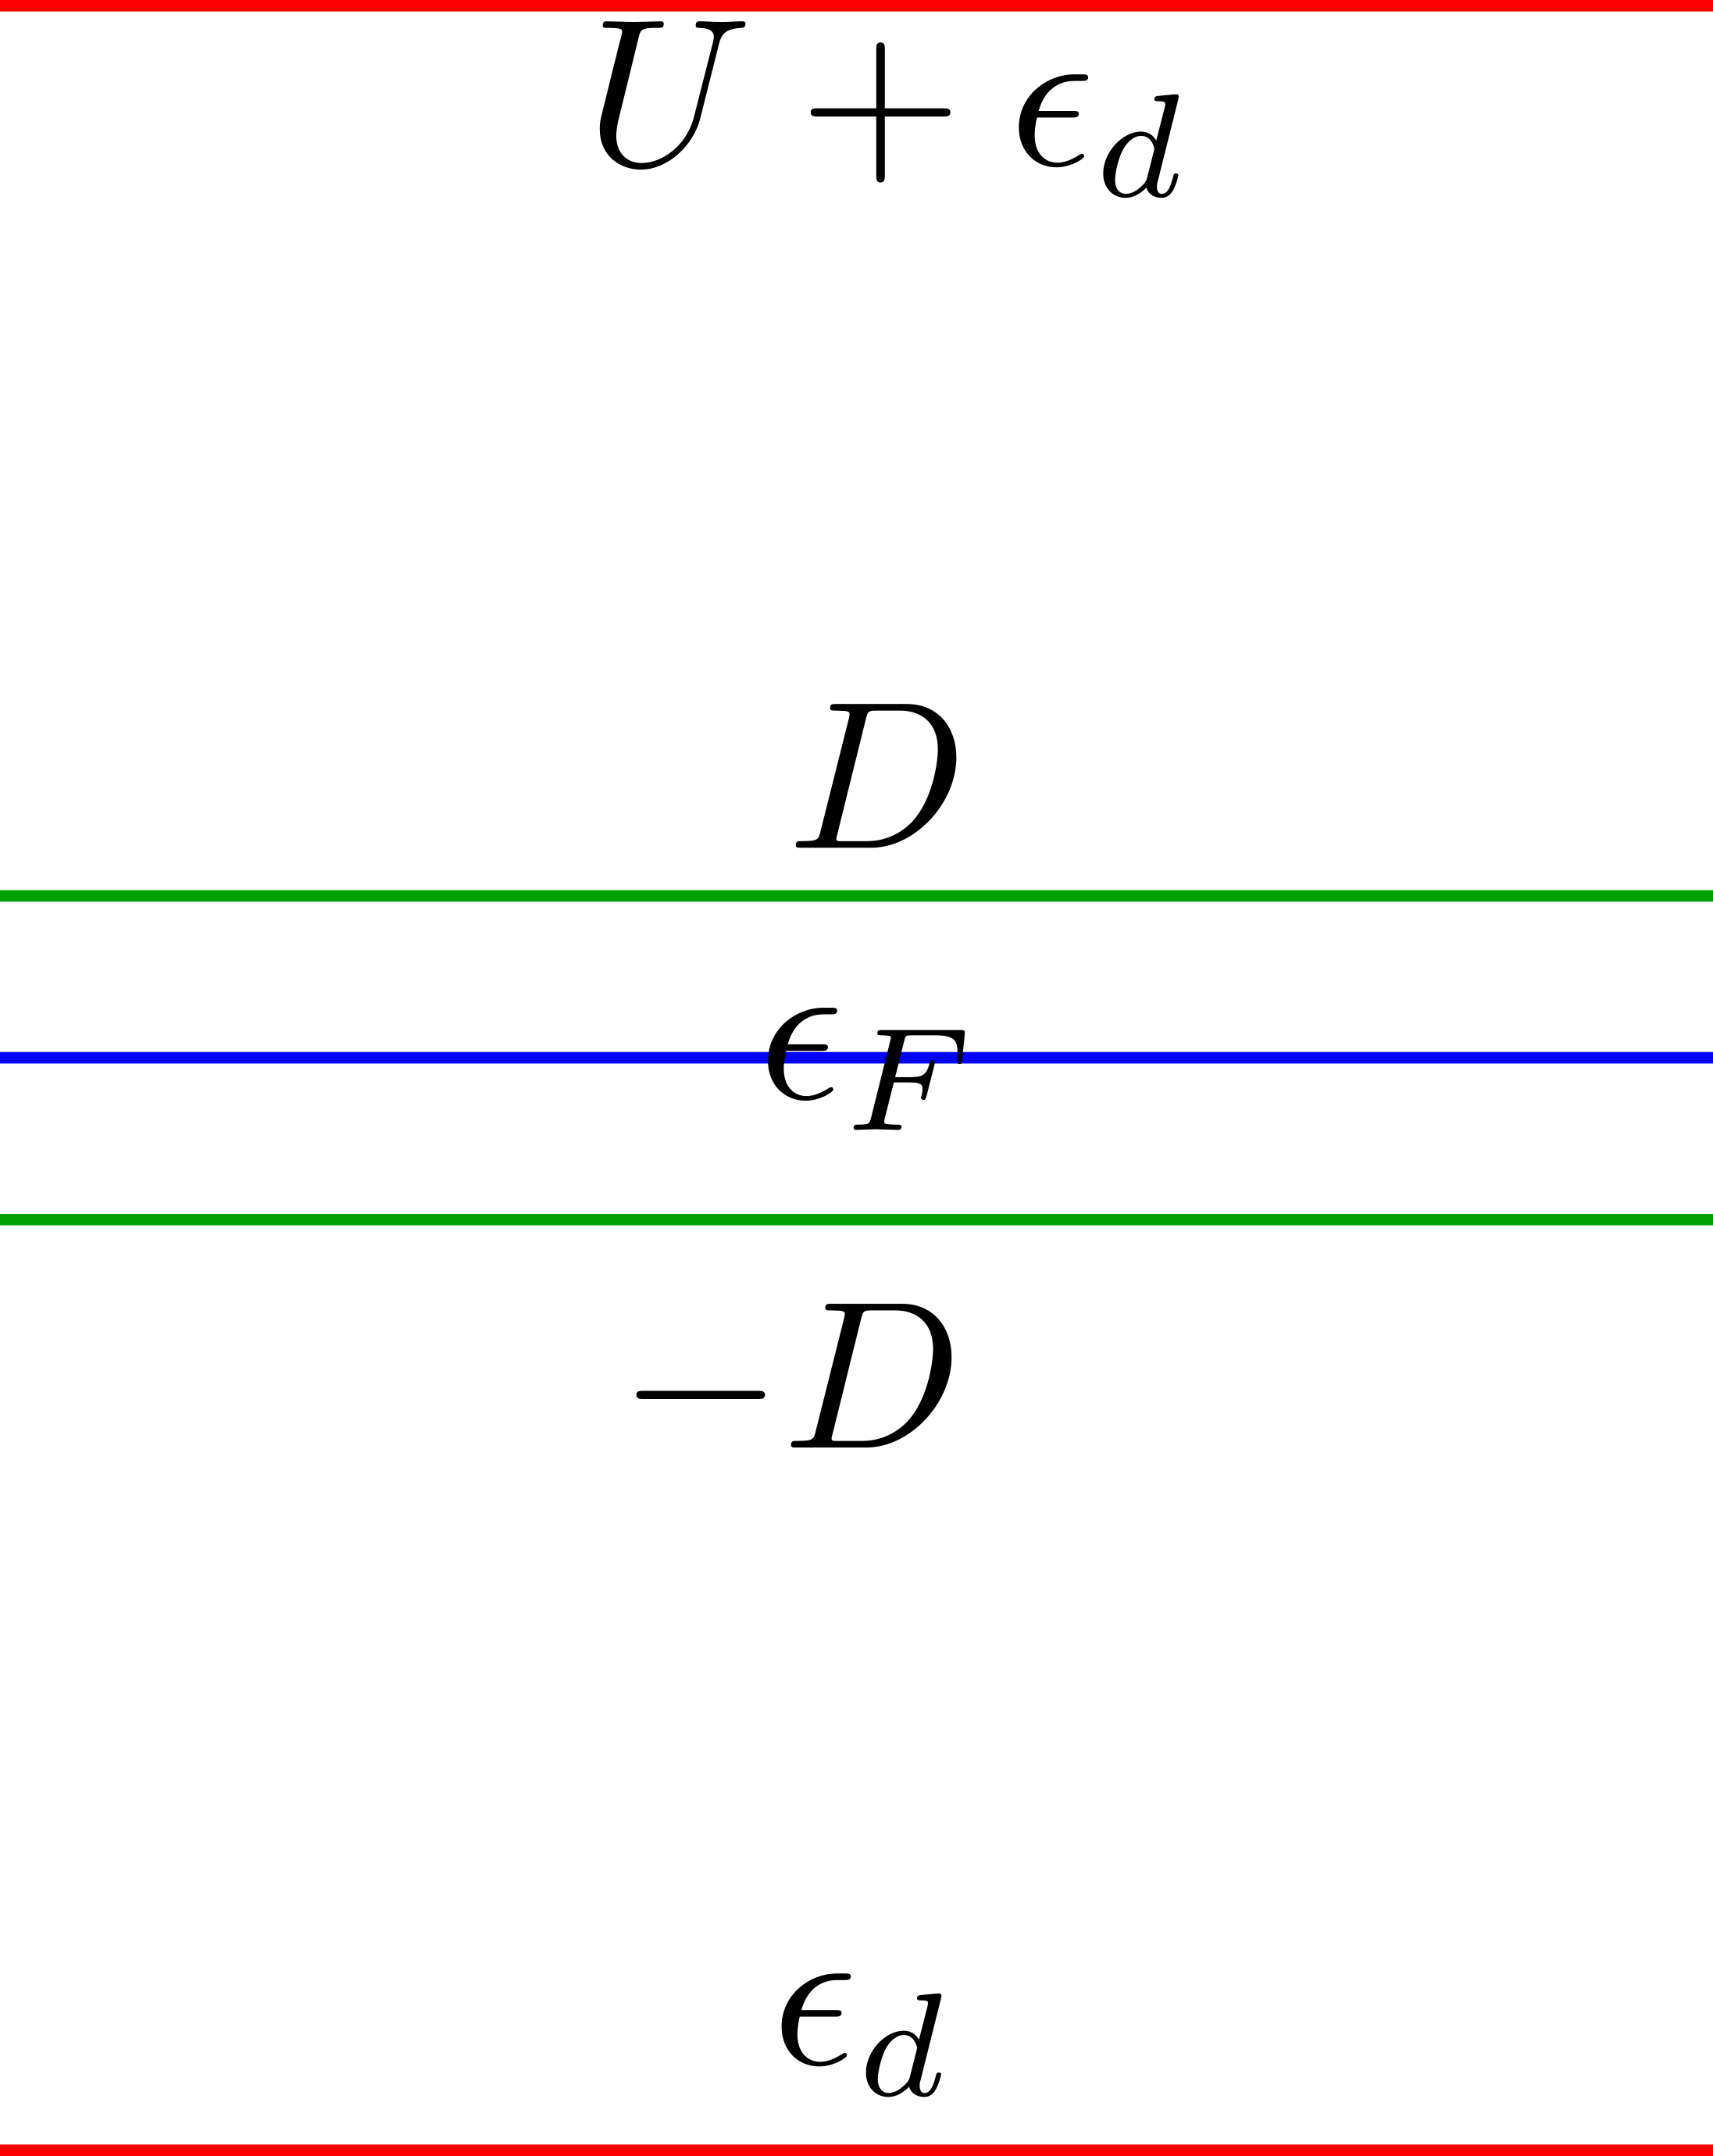
\includegraphics[scale=0.28]{anderson.png}}
	\hspace*{30pt}
	\subfloat[Subcaption 1]{\label{and2}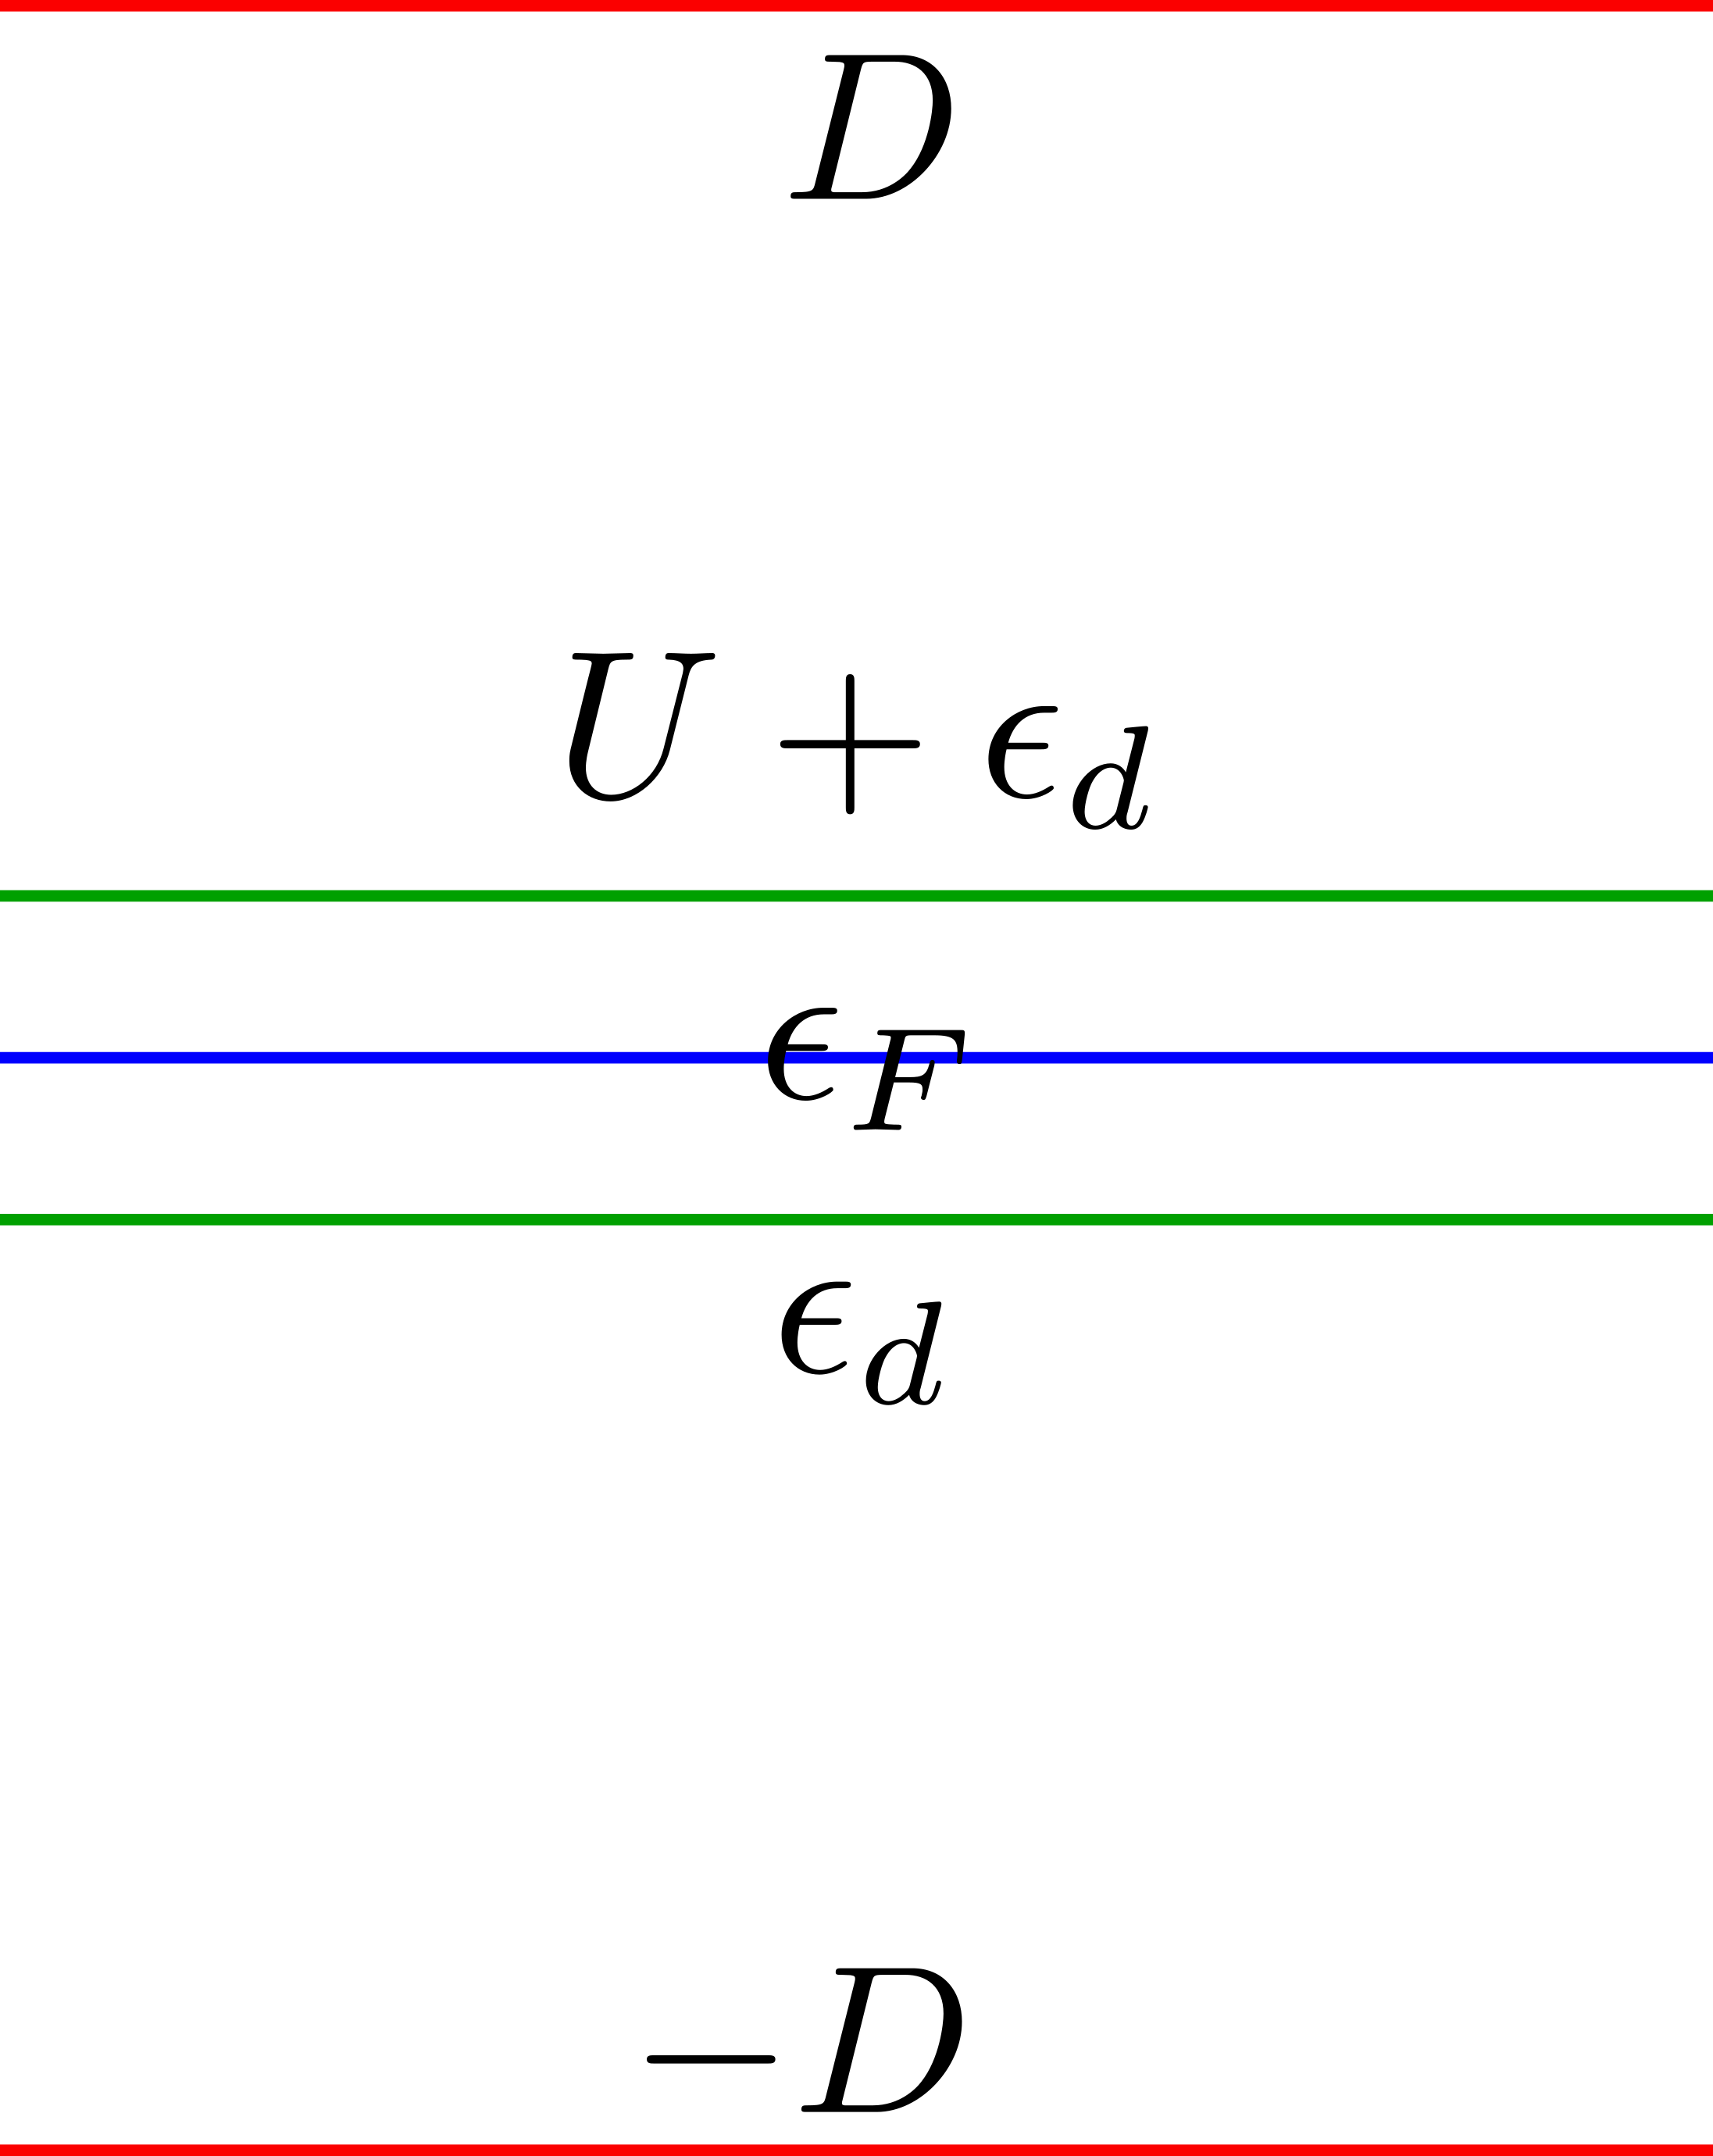
\includegraphics[scale=0.28]{anderson2.png}}
\end{figure}
%\begin{minipage}{220pt}
%	\centering
%	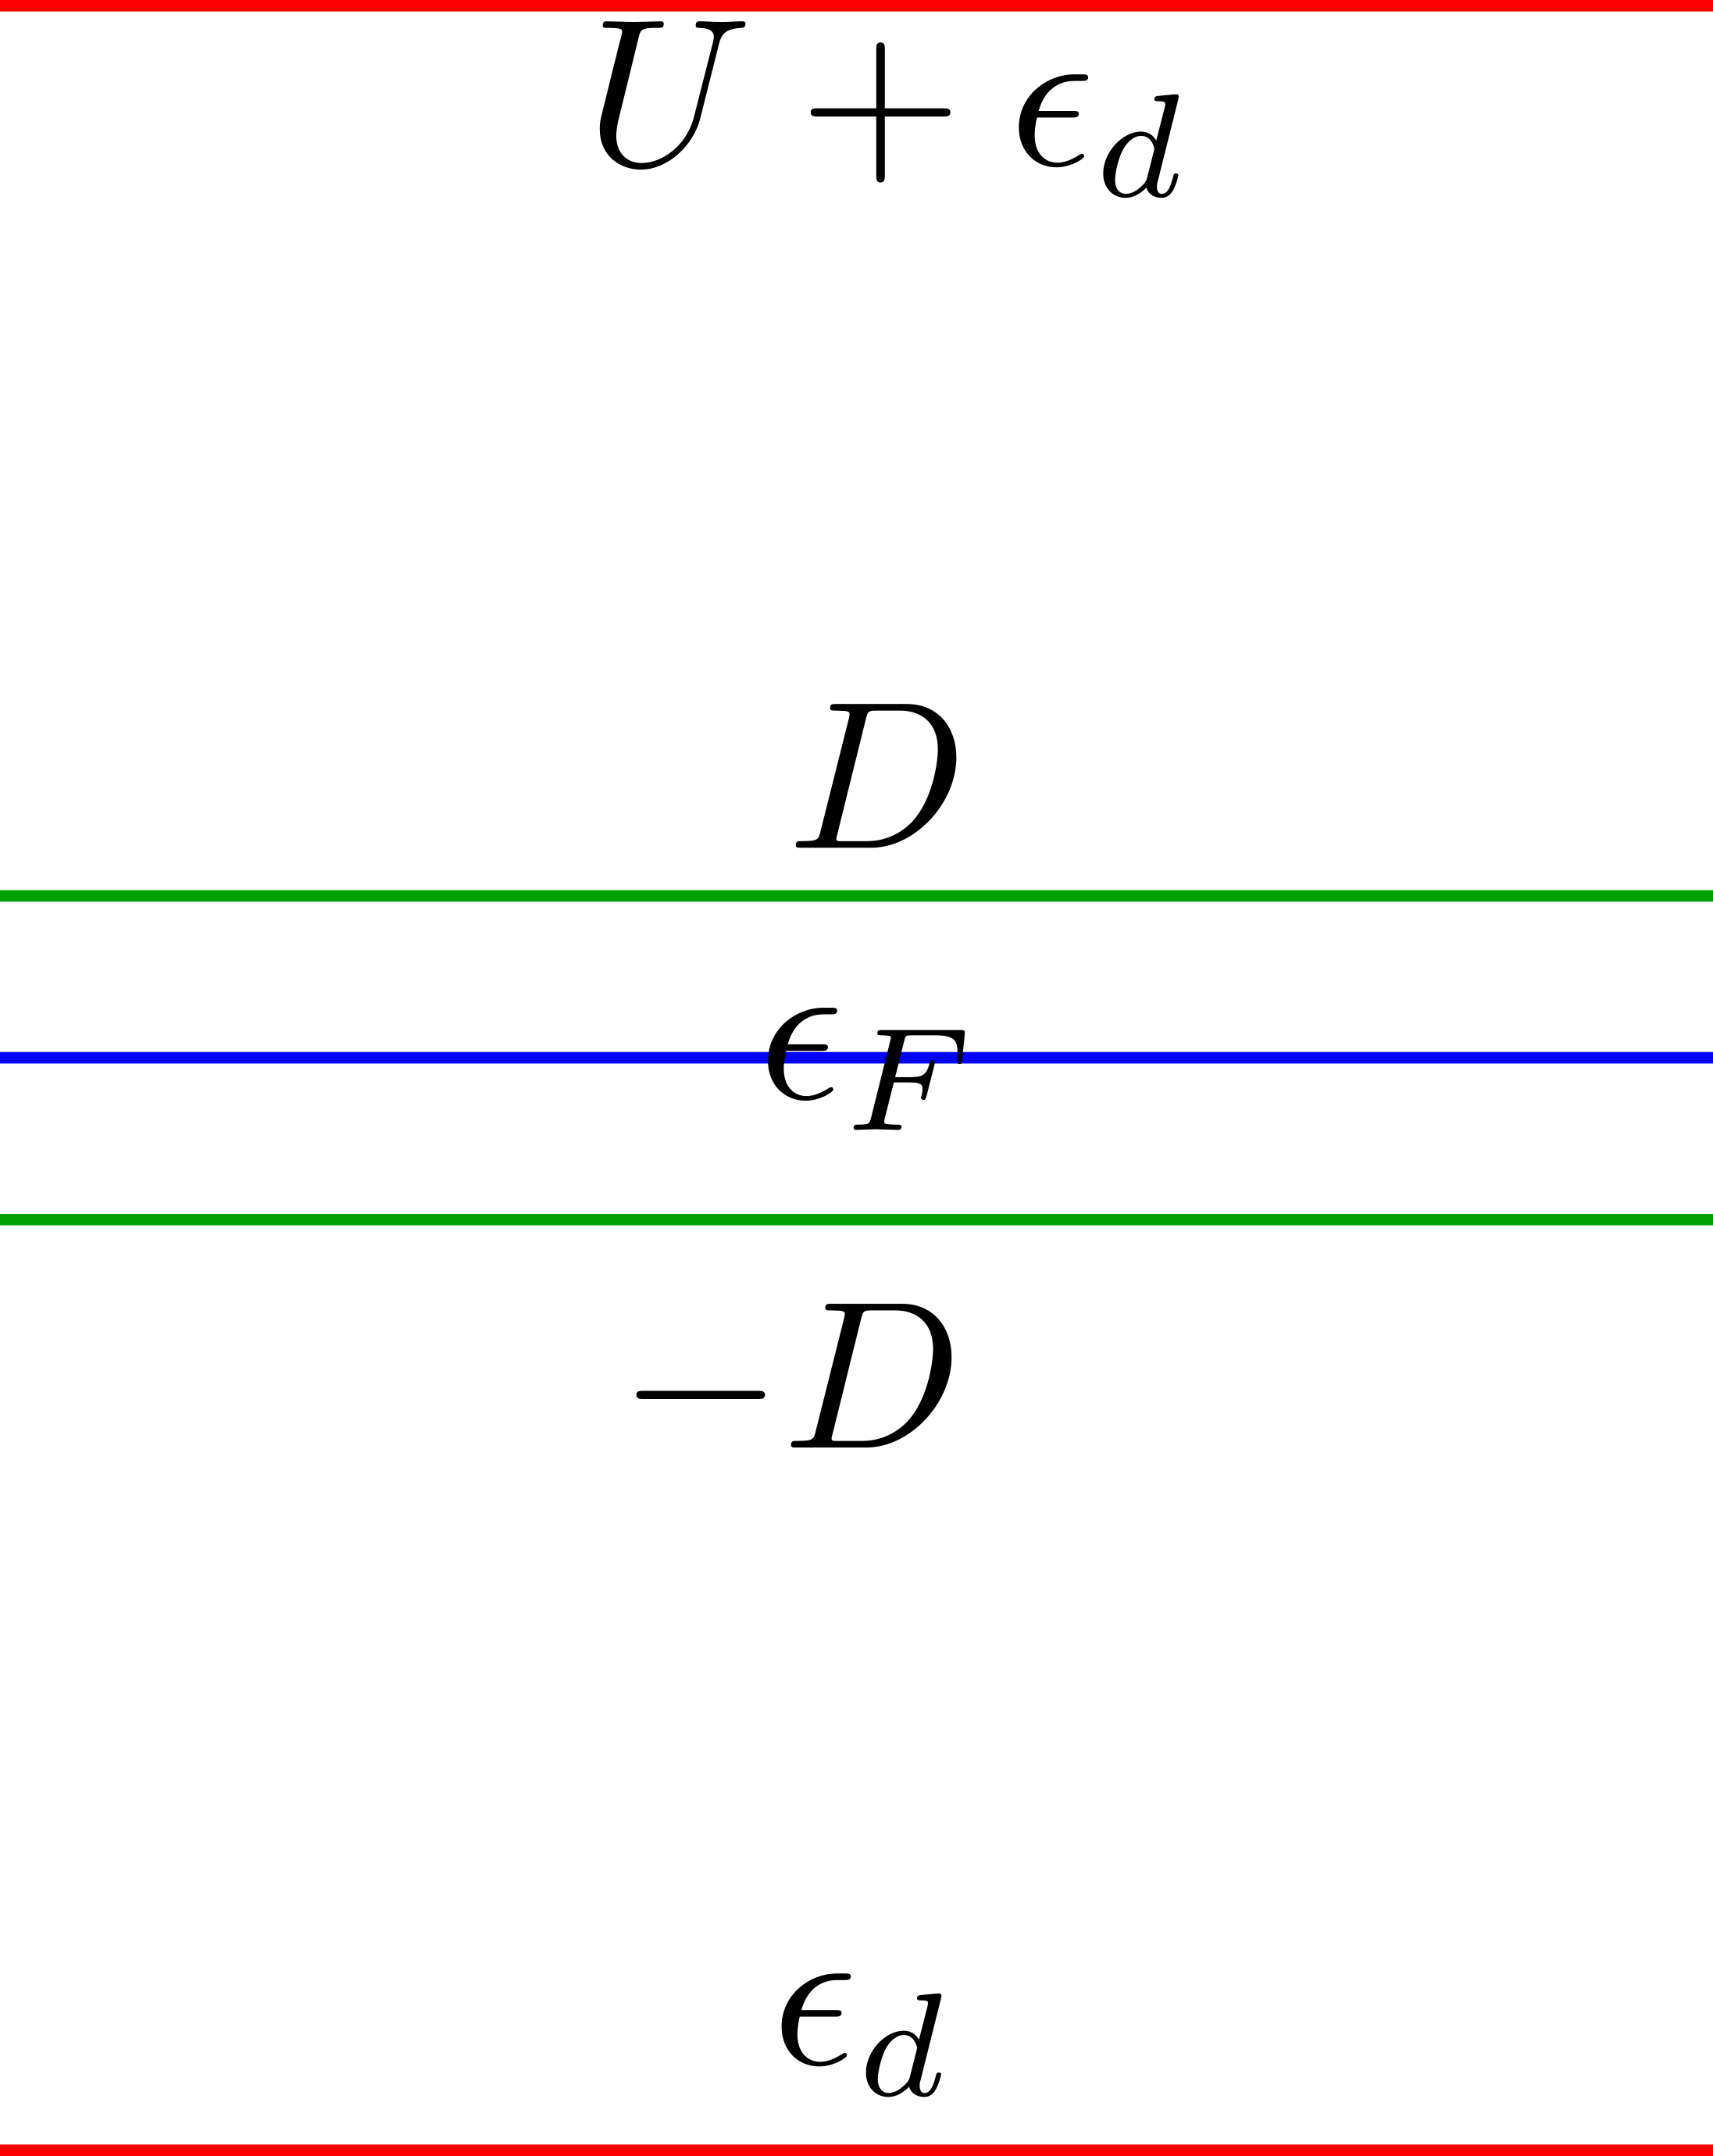
\includegraphics[scale=0.28]{anderson.png}
%	\captionof{figure}{Impurity levels outside}
%	\label{and1}
%\end{minipage}
%\begin{minipage}{220pt}
%	\centering
%	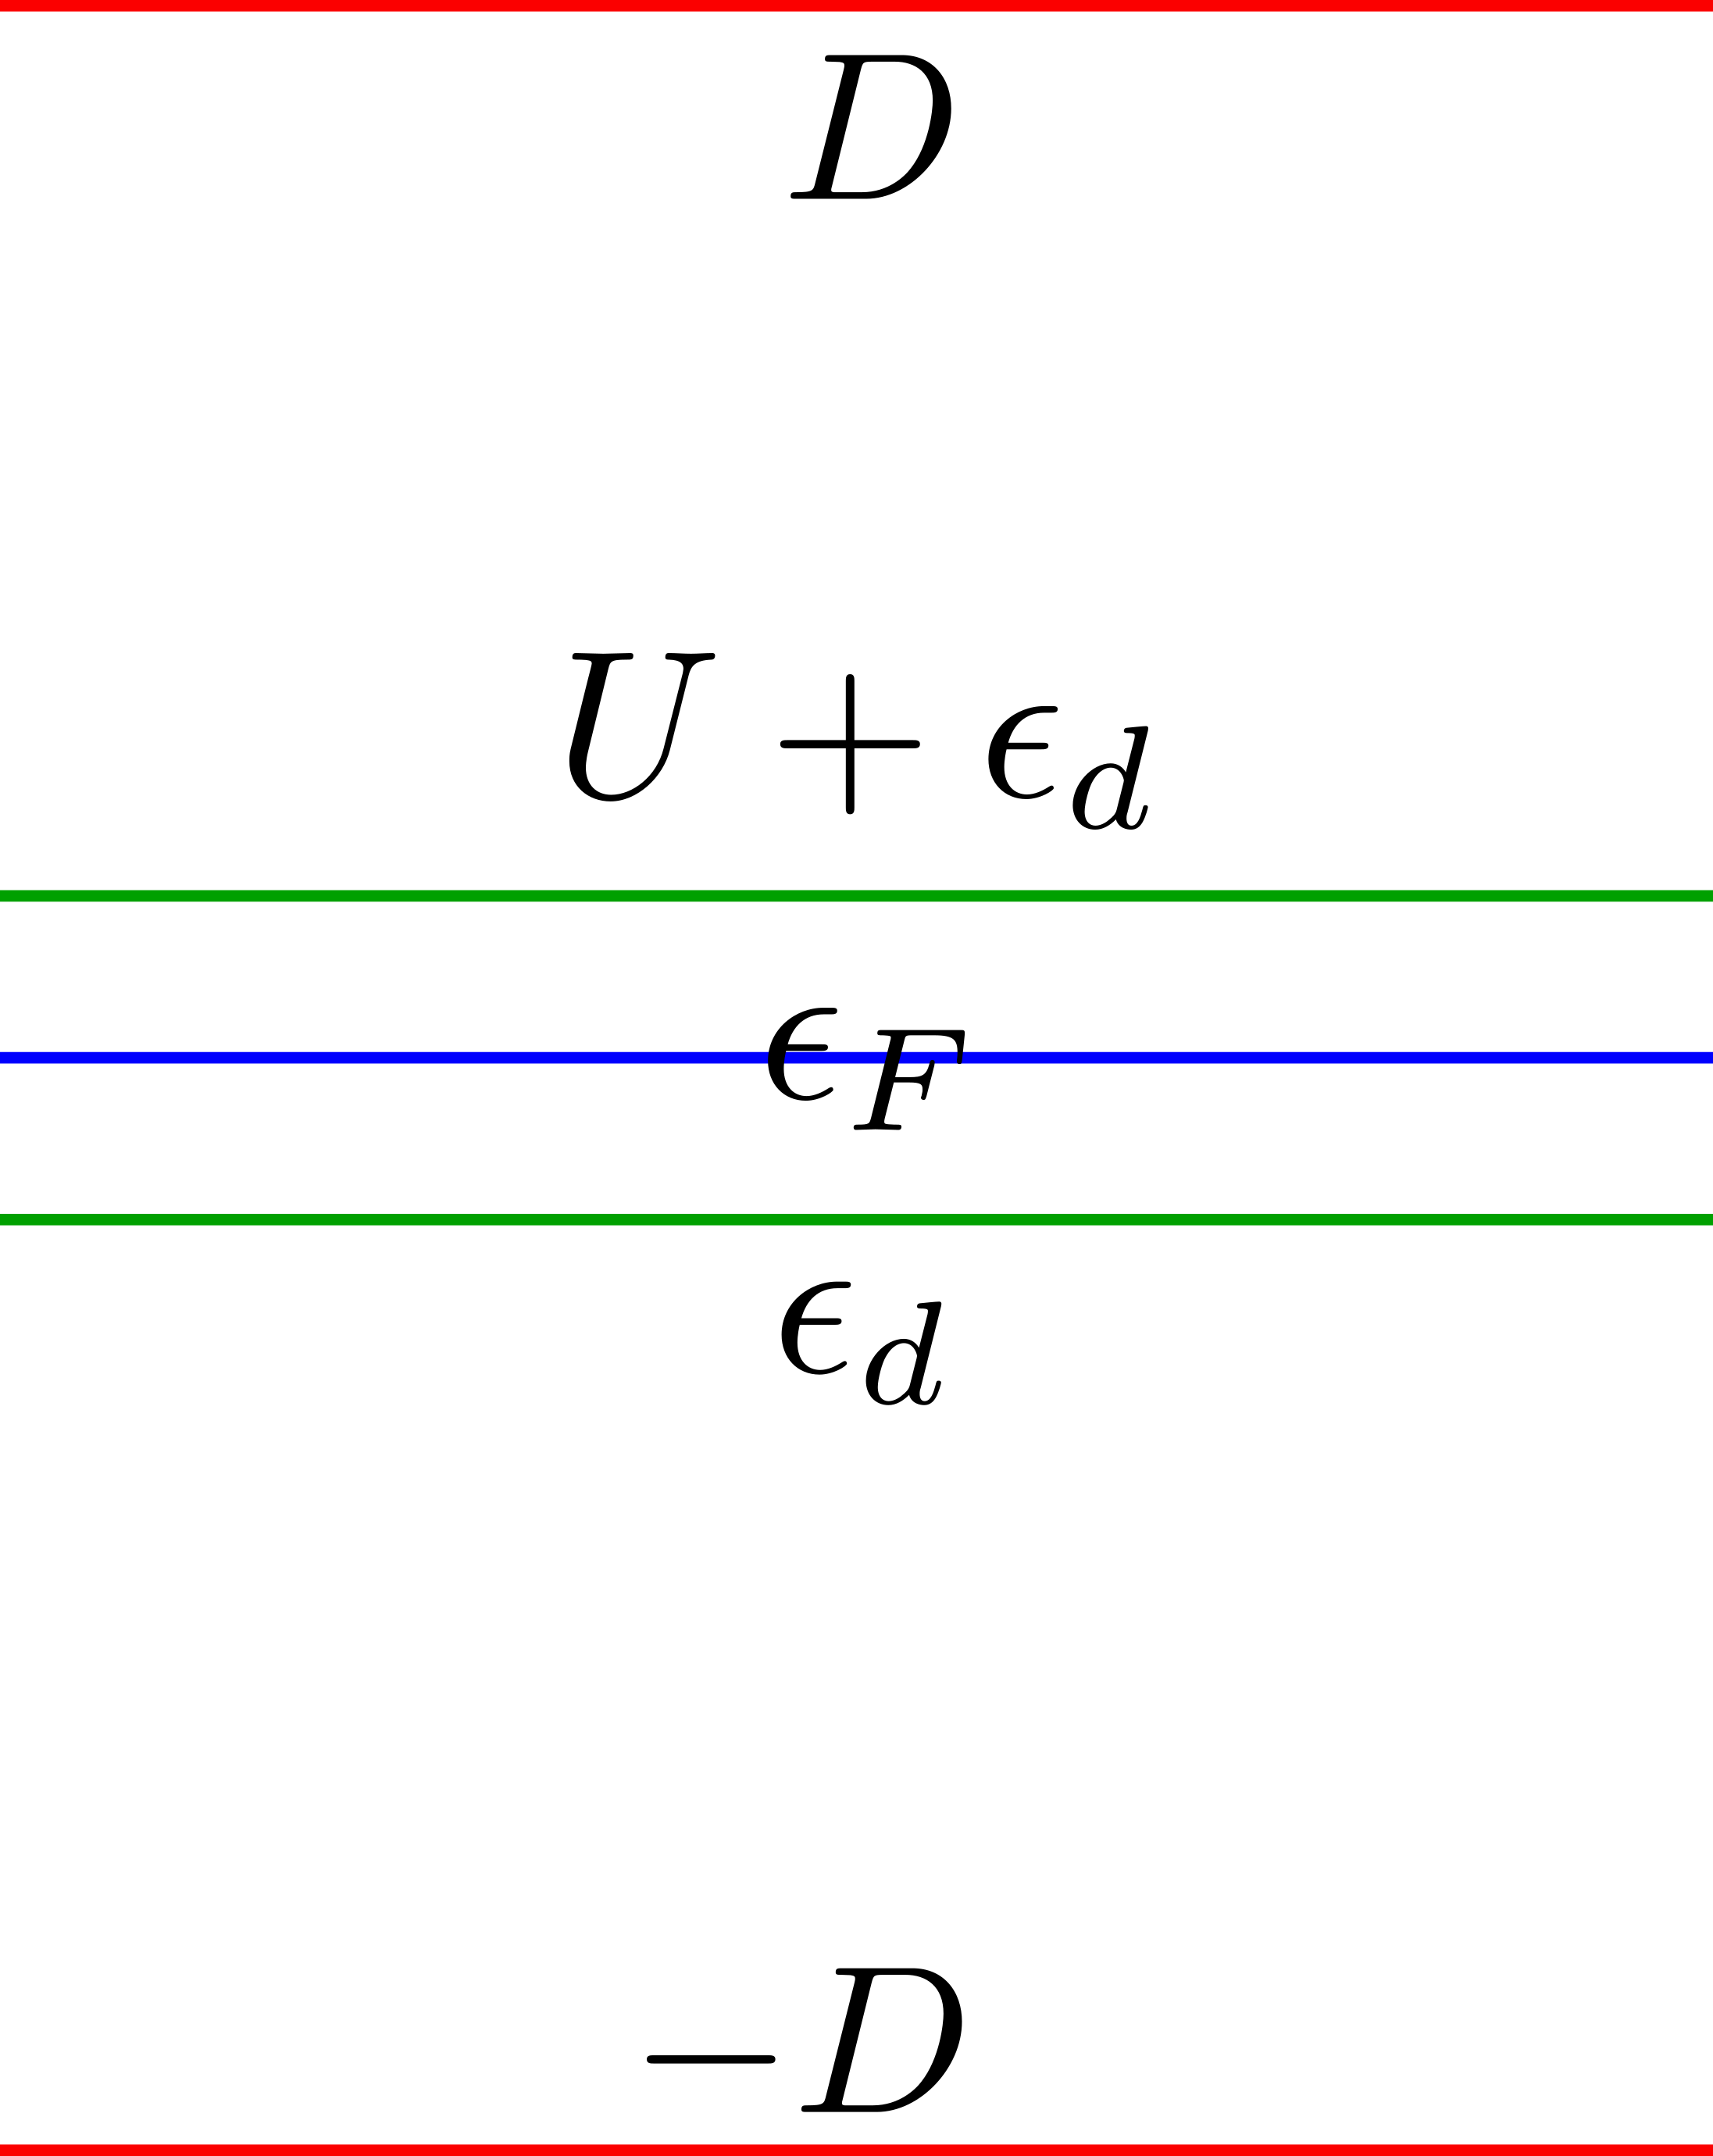
\includegraphics[scale=0.28]{anderson2.png}
%	\captionof{figure}{Impurity levels inside}
%	\label{and2}
%\end{minipage}
The limit where there will be some renormalization is the following.
We are working with the asymmetric Anderson model, that is,\\ \il{U + \epsilon_d \gg D \gg |\epsilon_d|,\Delta}.
The total Hamiltonian is
\beq
H = \sum_{k\sigma} \epsilon_{k\sigma}n_{k\sigma} + \epsilon_d \sum_\sigma n_{d\sigma} + U n_{d\ua}n_{d\da} + \sum_{k\sigma}\rr{V_{kd} c^\dagger_{k\sigma}c_{d\sigma} + V^*_{kd}c^\dagger_{d\sigma}c_{k\sigma}}
\eeq
This means that the doubly-occupied state is decoupled from the conduction band; it cannot hybridize through the \il{V_{kd}} because the virtual transition will involve a huge amount of energy and so it is practically impossible.\\\\
At the first iteration, we will reduce the cut-off from \il{D} to \il{D - \delta D}.
The zeroth approximation to this Hamiltonian is
\beq
H^{(0)} = \sum_{k<D-\delta D, \sigma} \epsilon_{k\sigma}n_{k\sigma} + \epsilon_d \sum_\sigma n_{d\sigma} + \sum_{k<D-\delta D,\sigma}\rr{V_{kd} c^\dagger_{k\sigma}c_{d\sigma} + V^*_{kd}c^\dagger_{d\sigma}c_{k\sigma}}
\eeq
As is apparent, the zeroth approximation involves completely ignoring the region to be integrated out.
All kinetic energies and actual scatterings are strictly within the smaller region \il{[-D + \delta D, D - \delta D]}.
The higher approximations  allow these states to make virtual transitions to the band edge states and then come back.
The Hamiltonian term for the virtual excitation in to the upper band edge (with a particle in the intermediate state) is
\beq
H^{(1,p)}_\sigma = \sum_{k\in k^+} \alpha_{k\sigma} c^\dagger_{d\sigma} c_{k\sigma}c^\dagger_{k\sigma} c_{d\sigma}
\eeq
There are two things to note here.
Firstly, \il{\alpha_{k\sigma}} is the probability of such a virtual transition and is found from perturbation theory.
Secondly, the summation \il{k^+} is over the states in \il{[D-\delta D,D]}.
To calculate \il{\alpha_{k\sigma}}, note that such a virtual excitation can take place only from the state \il{1_{d\sigma}}.
Therefore, we look at the first order correction to this state under the perturbation \il{V_{kd}}.
\beq
\alpha_{k\sigma} = \fr{\bra{1_{d\sigma}}V^*_{kd} c^\dagger_{d\sigma} c_{k\sigma}\ket{k\sigma}\bra{k\sigma}V_{kd}c^\dagger_{k\sigma} c_{d\sigma}\ket{1_{d\sigma}}}{E_{1_d\sigma} - E_{k\sigma}} = \fr{|V_{kd}|^2}{\epsilon_d - \epsilon_k}
\eeq
The analogous term in the same order for the virtual transition to the lower edge consists of a hole in the intermediate state, because the lower edge states are already filled.
This term is of the form
\beq
H^{(1,h)} = \sum_{k\in k^-,\sigma} \beta_{k\sigma} c^\dagger_{k\sigma} c_{d\sigma} c_{k\sigma} c_{d\sigma}^\dagger
\eeq
\il{\beta_{k\sigma}} is calculated similarly, using perturbation theory.

\beq
\beta_{k\sigma} = \fr{\bra{0}V^*_{kd} c_{d\sigma} c^\dagger_{k\sigma}\ket{k\sigma}\bra{k\sigma}V_{kd}c_{k\sigma} c^\dagger_{d\sigma}\ket{0}}{E_0 - E_{k\sigma}} = \fr{|V_{kd}|^2}{\epsilon_k - \epsilon_d}
\eeq
The total first order  correction to the Hamiltonian is of the form
\beq
H^{(1)} = \sum_{k^+,\sigma}\alpha_{k\sigma} T^+_{k\sigma} + \sum_{k^-,\sigma}\beta_{k\sigma} T^-_{k\sigma}
\eeq
\il{T^{+,-}} represent virtual transitions to the upper and lower edges.
Since these terms do not cause any real fluctuations in the impurity sites, they renormalize only the impurity energy \il{\epsilon_d}, and not the hybridisation coupling \il{V_{kd}}.
To find the renormalization in the site energies \il{\epsilon_0} and \il{\epsilon_1} (and hence in \il{\epsilon_d \equiv \epsilon_1 - \epsilon_0}), note that the term \il{T^+} virtually excites the state \il{n_{d\sigma} = 1}, and hence the change in \il{\epsilon_{1}} is
\beq
\delta \epsilon_{1} = \alpha_{k\sigma} = \sum_{k^+}\fr{|V_{kd}|^2}{\epsilon_d - \epsilon_k}
\eeq
We can write this summation in terms of \il{\Delta(E) = \pi N(E) V^2(E)}, under the assumption \il{\Delta (E) \approx \Delta} for \il{E \in \{-D,D\}}.
\beq
\delta \epsilon_{1} =\sum_{k^+}\fr{|V_{kd}|^2}{\epsilon_d - \epsilon_k} = \int_{D-\delta D}^{D} dE N(E) \frac{|V(E)|^2}{\epsilon_d - E} \approx \frac{\Delta}{\pi}\fr{ |\delta D|}{\epsilon_d - D}
\eeq
The change in \il{\epsilon_0} is
\beq
\delta \epsilon_{0} = \sum_\sigma \beta_{k\sigma} \approx -2\frac{\Delta}{\pi}\fr{ |\delta D|}{\epsilon_d + D}
\eeq
The change in the denominator occurs because in the lower edge, \il{\epsilon_k = -D}.
 The change in \il{\epsilon_d} is
\beq
\delta \epsilon_d = \delta \epsilon_1 - \delta \epsilon_0 = \fr{\Delta |\delta D|}{\pi}\qq{\fr{1}{\epsilon_d - D} + \fr{2}{\epsilon_d +D}} = \fr{\Delta}{\pi}\fr{|\delta D|}{D} = -\fr{\Delta}{\pi}\delta\ln D
\eeq
We assumed \il{D \gg \epsilon_d}.
In the limit of infinitesimal change, we get the equation
\beq[scale_eq]
\dv{\epsilon_d}{\ln D} = -\fr{\Delta}{\pi}
\eeq
If we had allowed the \il{\ket{1_{d\sigma}}} to hybridize with the state \il{\ket{2_d}} (that is, if we had assumed both \il{U} and \il{\epsilon_d} to be \il{\ll D}), then \il{\alpha_{k\sigma}} would have had another term added to it:
\beq
\fr{|V_{kd}|^2}{\epsilon_k - U -\epsilon_d} \approx  \fr{|V|^2}{-D - U -\epsilon_d}
\eeq
\il{-(U+\epsilon_d)} is the change in energy from \il{\ket{1_d}} to \il{\ket{2_d}} and \il{-D} is the energy of the hole created in the process.
The renormalization in \il{\epsilon_d} would then have been
\beq
\delta \epsilon_d = \fr{\Delta |\delta D|}{\pi}\rr{\fr{1}{\epsilon_d - D} - \fr{1}{D + U + \epsilon_d} + \fr{2}{\epsilon_d + D}}
\eeq
which is zero in the limit of \il{U,|\epsilon_d| \ll D}.
This is the equal renormalization in \il{\epsilon_0} and \il{\epsilon_1} discussed earlier.\\\\
We do not yet know whether \il{\Delta} is a function of the cutoff \il{D}.
To find the renormalization of \il{\Delta}, we need to find the renormalization of \il{V_{kd}}.
Note that the lowest order virtual transitions do not cause any actual charge fluctuation, and hence they do not renormalize \il{V_{kd}}.
To see the renormalization of \il{V_{kd}}, we need to consider one order higher.
These higher order terms involve transitions within the lower subspace along with virtual transitions into the higher subspaces.
\beq
H^{(2)} = \sum_{k^+,q,\sigma}\alpha_{k\sigma} T^+_{k\sigma}\gamma_{q,k,\sigma}c^\dagger_{d\sigma}c_{q\sigma} + \sum_{k^-,q,\sigma}\beta_{k\sigma} T^-_{k\sigma}\gamma_{q,k,\sigma}c_{d\sigma}c^\dagger_{q\sigma}
\eeq
The \il{\gamma_{k\sigma}} can be calculated as 
\beq
\alpha_{k\sigma}\gamma_{q,k,\sigma} = \fr{\bra{1_{d\sigma}}V^*_{kd} c^\dagger_{d\sigma} c_{k\sigma}\ket{k\sigma}\bra{k\sigma}V_{kd}c^\dagger_{k\sigma} c_{d\sigma}\ket{1_{d\sigma}}\bra{1_{d\sigma}}V_{kd}c_{q\sigma} c^\dagger_{d\sigma}\ket{q\sigma}}{(E_{1_d\sigma} - E_{k\sigma})(E_q - E_k)} \\
= \alpha_{k\sigma}\fr{V_{kd}}{\epsilon_q - \epsilon_k}
\eeq
The renormalization in \il{V_{kd}} is therefore
\beq
\delta V_{kd} = \fr{\Delta}{\pi}\fr{|\delta D|}{\epsilon_d - D}\fr{V_{kd}}{\epsilon_q - \epsilon_k}
\eeq
Close to the band edge, we get
\beq
\delta V = \fr{\Delta}{\pi}\fr{|\delta D|}{\epsilon_d - D}\fr{V}{\epsilon_q - D} \approx \fr{\Delta}{\pi}\fr{|\delta D|}{D^2}V
\eeq
Therefore,
\beq[mirai2]
\delta \Delta \sim V\delta V = \fr{\Delta V^2}{\pi D^2}|\delta D| \implies \dv{\Delta}{D} \sim \rr{\fr{\Delta}{D}}^2
\eeq
For \il{D \gg \Delta}, this will vanish very quickly.
Hence, in this regime, there is no renormalization of \il{\Delta}, and we can take it to be a constant in the renormalization flow.
Integrating eq.~\ref{scale_eq} gives
\beq
\epsilon_d = -\fr{\Delta}{\pi}\ln D + \text{constant}
\eeq
Defining the constant as 
\beq
\text{constant} = \epsilon_d^* + \fr{\Delta}{\pi}\ln \Delta
\eeq
we get
\begin{gather}
\epsilon_d = -\fr{\Delta}{\pi}\ln D +  \epsilon_d^* + \fr{\Delta}{\pi}\ln \Delta \\
\implies \epsilon_d = \epsilon_d^* - \fr{\Delta}{\pi}\ln \fr{D}{\Delta}\label{const}
\end{gather}
This result is in the regime \il{U + \epsilon_d \gg D \gg |\epsilon_d|}.
Even if \il{U \ll D} initially, scaling will begin once \il{D \sim U}.
Until then, as mentioned previously, both \il{\epsilon_1} and \il{\epsilon_0} will change equally and there won't be any scaling in \il{\epsilon_d}.
If we start with \il{U \ll D}, under scaling, as \il{D} will decrease, there won't be any renormalization until we reach the point \il{D \sim U}.\\\\
Say, as a result of scaling, the bandwidth decreases and \il{\epsilon_d} increases (which it will, as is apparent from the eq.~\ref{const}).
At some point, \il{-D \lesssim \epsilon_d}.
At this point, perturbation theory breaks down and we resort to SWT.
We denote this point of the scaling by \il{D = -a\wl \epsilon_d, a > 1}.
We can then express the SWT coupling constant \il{\wl J} by replacing \il{\epsilon_d} with \il{\wl \epsilon_d} in eq.~\ref{jexpr}.
For simplicity set \il{U = \infty}.
Then,
\beq[historia]
\wl J = -\fr{|V|^2}{\wl \epsilon_d} = \fr{a|V|^2}{D}
\eeq
We can then do the poor man's scaling with this coupling.
From eq.~\ref{sol},
\beq
T_K \sim D \sqrt{\wl J N(0)^2} \ex{-\fr{1}{2 \wl J N(0)^2}} = \sqrt{\Delta D}\ex{-\fr{D}{2\Delta}}\\
\sim D\sqrt{\fr{\Delta}{D}}\ex{\fr{\epsilon_d}{2\Delta}}
\eeq
A different result is obtained if one is in the regime of \il{\epsilon_d < -D}.
This is the situation mentioned at the very beginning of the discussion, fig.~\ref{and1}.
Assuming \il{U \ra \infty} and \il{\epsilon_d} outside the conduction band, we can do a SWT and the \il{T_K} obtained is q.~\ref{sol},
\begin{gather}
	J = -\fr{V^2}{\epsilon_d}\\
	g = J\rho = -\fr{\Delta}{\epsilon_d}\\
	\implies T_K = D\sqrt{\fr{\Delta}{\epsilon_d}}\ex{\fr{\epsilon_d}{2\Delta}}\label{jean2}
\end{gather}
The two forms of the Kondo temperature show that the prefactor is not a universal function; it depends on the starting conditions (the microscopic Hamiltonian from which we start the scaling).
But the universal fact is that in the local moment regime (\il{U \ra \infty}), all physical quantities will involve only one energy scale, \il{T_K}.
This \il{T_K} itself might be different based on the starting Hamiltonian.\\\\
For \il{\epsilon_d^* \gg \Delta}, the renormalization will stop at \il{D \sim \epsilon_d}.
Note that we had assumed \il{D \gg \epsilon_d}.
That was the starting condition, that is, \il{\epsilon_d} deep inside the Fermi surface.
During the renormalization, \il{D} will keep on decreasing and \il{\epsilon_d} will continuously increase.
At some value of \il{D}, they will become equal and the impurity level will go outside the Fermi surface.
At this point, none of the impurity levels can renormalize any more, because the relevant energy scales are greater than the cutoff.
Hence the renormalization stops at this point.
\begin{figure} \centering 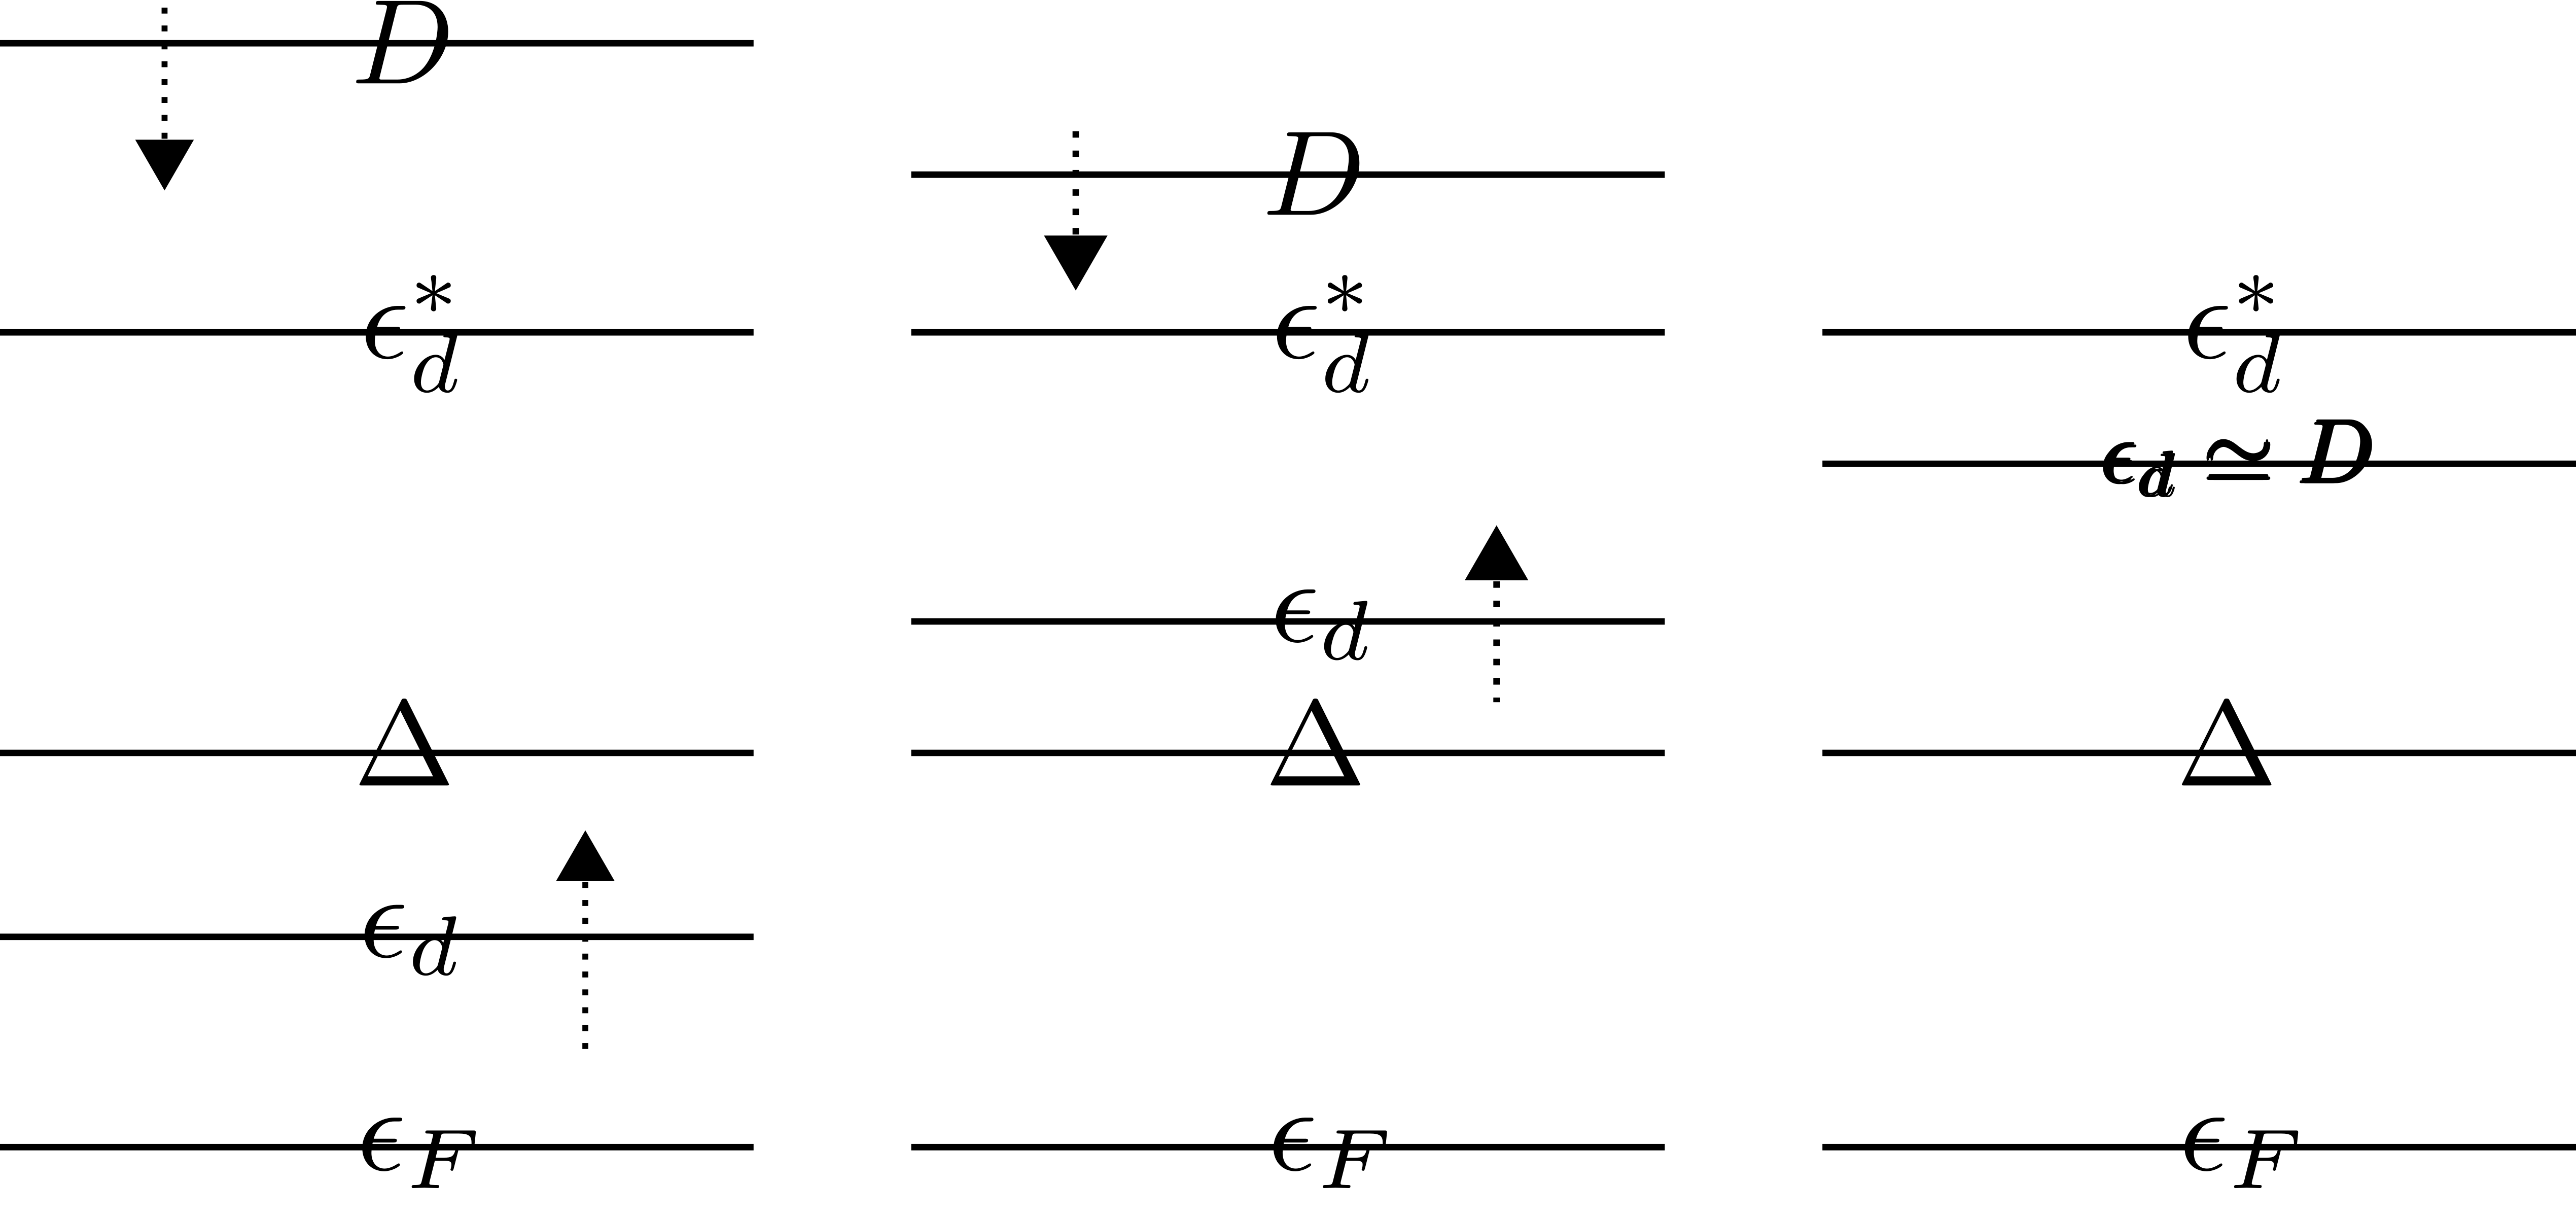
\includegraphics[scale=0.29]{full.png}\caption{Renormalization in the energy levels when \il{\epsilon_d^* \gg \Delta}}\end{figure}
This point is given by \il{\ol D = a\epsilon_d(\ol D) \equiv \ol \epsilon_d} where \il{a} is a constant of order unity.
It satisfies the equation
\beq[eraser]
\ol \epsilon_d = \epsilon_d^* - \fr{\Delta}{\pi}\ln \fr{a\ol \epsilon_d}{\Delta}
\eeq
which is just eq.~\ref{const} with the substitution \il{D =a  \ol \epsilon_d}.
In this regime, because \il{\epsilon_d \gg \Delta}, we can do a perturbative expansion of the  bare Hamiltonian in terms of \il{\fr{\Delta}{\epsilon_d}}.
The susceptibility is
\beq
\chi_d = \fr{\Delta}{2\pi}\rr{\fr{g \mu_B}{\epsilon_d}}^2\qq{1 + \fr{2\Delta}{\pi \epsilon_d}\ln \fr{\epsilon_d}{D} + ...}
\eeq
From the scaling, we know that \il{D} can be decreased to \il{\ol D}.
We can hence substitute \il{D =a \ol \epsilon_d, \epsilon_d = \ol \epsilon_d}.
With this in mind, the susceptibility becomes
\beq
\chi_d = \fr{\Delta}{2\pi}\rr{\fr{g \mu_B}{\ol\epsilon_d}}^2\qq{1 + \fr{2\Delta}{\pi \ol\epsilon_d}\ln a + ...} \\
= \fr{\Delta}{2\pi}\rr{\fr{g \mu_B}{\ol \epsilon_d}}^2\qq{1 +\text{O}\rr{\fr{2\Delta}{\pi \ol\epsilon_d}}}
\eeq
where I used the fact that \il{\ln a } will be of order 1.
As we go on decreasing the cutoff, the impurity level will go on moving farther away from the Fermi level, and impurity site will become null occupied: \il{\avg{n_d} \approx 0}.
The critical cutoff \il{\ol D} can be associated with a temperature  scale \il{k_b \ol T = \ol D}.
At temperatures sufficiently below this temperature (\il{T \ll \ol T}), the susceptibility becomes (again from perturbation theory)
\beq
\chi_d(T) = \fr{\Delta}{2\pi}\rr{\fr{g \mu_B}{\ol \epsilon_d}}^2 + \fr{1}{4T}\qq{1+\hf\ex{\fr{T^*}{T}}}^{-1}
\eeq
For temperatures sufficiently low, which we demarcate by a temperature \il{T_{FL}}, the denominator in the second term will be sufficiently large so that we can ignore that term with respect to the first term:
\beq
T \gg T_{FL} \implies e^\fr{T^*}{T} \gg 1 \implies \qq{1+\hf\ex{\fr{T^*}{T}}}^{-1} \approx 0 
\eeq
The susceptibility in this low temperature range can thus be written as
\beq[sakura]
\chi_d = \fr{\Delta}{2\pi}\rr{\fr{g \mu_B}{\ol \epsilon_d}}^2
\eeq
This is analogous to the  result obtained in eq.~\ref{mimp}, from the mean field version of the Fermi liquid theory, and also obtained from a renormalized perturbation theory of Anderson model.
To see how, note that since we are in the limit \il{\avg{n_d} = 0}, the onsite repulsion term \il{U} can be dropped because there is no probability of double occupation.
Eq.~\ref{mimp} then becomes
\beq[sasuke]
\chi_d = \fr{g^2 \mu_B^2}{2} \rho_d(0) = \fr{g^2 \mu_B^2}{2} \fr{\Delta}{\pi}\fr{1}{\ol \epsilon_d^2 + \Delta^2}
\eeq
Next note that we had assumed at the beginning that \il{\epsilon_d^* \gg \Delta}.
We need to find the relative order difference between \il{\ol \epsilon_d} and \il{\Delta}.
From eq.~\ref{eraser}, we can drop the \il{\pi} and \il{a} because they are of order 1.
\beq
\ol \epsilon_d = \epsilon_d^* - \Delta \ln \fr{\ol \epsilon_d}{\Delta}
\eeq
Dividing through by \il{\Delta} and defining \il{x_1 = \fr{\ol \epsilon_d}{\Delta}, x_2 = \fr{\epsilon_d^*}{\Delta}}, we get
\beq
x_1 + \ln x_1 = x_2
\eeq
Since \il{O(\ln x_1) \leq O(x_1)}, we can write
\begin{gather}
O(x_1) = O(x_2)\\
\implies O\rr{\fr{\ol \epsilon_d}{\Delta}} = O\rr{\fr{\epsilon_d^*}{\Delta}}\\
\implies O\rr{\ol \epsilon_d} = O\rr{\epsilon_d^*}\\
\end{gather}
Since \il{\ol \epsilon_d} and \il{\epsilon_d^*} are of the same order, we can say:
\beq
\epsilon_d^* \gg \Delta \implies \ol \epsilon_d \gg \Delta
\eeq
Applying this to eq.~\ref{sasuke} means
\beq
\chi_d \approx \fr{g^2 \mu_B^2}{2} \fr{\Delta}{\pi}\fr{1}{\ol \epsilon_d^2}
\eeq
which is the same as eq.~\ref{sakura}.
This tells us that scaling all the way down to very low temperatures in regime \il{\epsilon_d^* \gg \Delta} brings us into a Fermi liquid state, characterized by a temperature-independent susceptibility (as is standard in a Fermi liquid).
The crossovers can be seen by looking at the variation of the Curie constant \il{\chi T}.\\\\
Since the susceptibility is proportional to the magnetic moment, presence of degeneracy will reduce this moment because the probability of occupying the states will decrease.
As a result, the Curie constant is also a measure of the effective degeneracy of the impurity orbital.
At very high temperatures \il{T \gg U,\epsilon_d}, all the impurity levels \il{0,\epsilon_d} and \il{2\epsilon_d + U} will become degenerate on energy scales of the order of \il{k_B T}.
As a result, the Curie constant is approximately \il{\fr{1}{8}} in this range.
The impurity occupancy is \il{n_d = 1}, because there are 4 degenerate states and the average number of electrons on them is 1.
At lower temperatures \il{U \gg T \gg T^*}, the degeneracy gets lowered; now, only the vacant and single-occupied states are degenerate.
Here the Curie constant is \il{\fr{1}{6}}.
In this case, the average occupancy is \il{n_d = \fr{0+1+1}{3} = \fr{2}{3}}.
At still lower temperatures, we saw that the impurity becomes vacant and \il{n_d = 0}.
The Curie constant becomes linear in temperature, going down to 0.
More formally,
\beq[suscep]
m = \fr{1}{\beta}\pd{\ln Z}{B} \implies \chi = \lim_{B \to 0}\pd{m}{B} = \lim_{B \to 0}\fr{1}{Z^2\beta}\qq{Z\fr{\partial^2 Z}{\partial B^2} - \rr{\pd{Z}{B}}^2}
\eeq
For the case of four-fold degeneracy, all the states can be assumed to be at zero energy.
Then, under a magnetic field B (\il{h=\fr{g\mu_B}{2}B}), the partition function is
\begin{gather}
Z = 1 + \ex{\beta h} + \ex{-\beta h} + 1 = 2\rr{1+\cosh \beta h}\\
\implies \pd{Z}{B} = g \mu_B \beta \sinh \beta h\\
\implies \fr{\partial^2 Z}{\partial B^2} = \hf\rr{g \mu_B}^2 \beta^2 \cosh \beta h
\end{gather}
Since \il{\lim_{h \to 0} \sinh \beta h = 0} and \il{\lim_{h \to 0} \cosh \beta h = 1}, we get
\begin{gather}
\chi = \fr{\beta g^2 \mu_B^2}{2 Z(h=0)}
\end{gather}
Setting \il{g \mu_B = k_B = 1}, we get
\beq[suscdeg]
\chi T =\fr{1}{2\mc{D}}
\eeq
where \il{Z(h=0) = 2 + 2 = 4 = \mc{D}} is the degeneracy.
\\\\
Similarly, for the triplet case (\il{\epsilon_d} and 0 are degenerate while \il{U \gg T}), the doubly occupied case is essentially cut off from the available states, so \il{Z = 1 + 2\cosh \beta h}.
The proof again goes through similarly.
But this time, we have \il{Z(h=0) = 1 + 2 = 3 = \mc{D}}.\\\\
For \il{\epsilon_d = k_B T^* > k_B T} such that \il{k_B T^* \gg \Delta}, we can find the magnetic moment in a perturbative fashion.
At the zeroth order, we can neglect the hybridisation \il{\Delta}.
Then,
\beq
m^{(0)} = \fr{1}{\beta}\pd{\ln Z(h)}{B}
\eeq
where
\beq
Z(h) = 1 + e^{-\beta\rr{k_B T^* -h}}+ e^{-\beta\rr{k_B T^* +h}} = 1 + e^{-\fr{\beta}{\beta^*}}2\cosh \beta h
\eeq
Therefore,
\beq
\chi^{(0)} = \lim_{h \to 0} \fr{1}{\beta Z}\fr{\partial^2 Z}{\partial B^2} = \lim_{h \to 0} \fr{g^2 \mu_B^2}{4 \beta Z}\fr{\partial^2 Z}{\partial h^2} = \fr{g^2 \mu_B^2}{4}\beta \fr{2e^{-\fr{\beta}{\beta^*}}}{1 + 2e^{-\fr{\beta}{\beta^*}}}
\eeq
Again setting \il{g \mu_B = k_B = 1}, we get,
\beq
\chi^{(0)} = \fr{1}{4 T} \fr{2e^{-\fr{\beta}{\beta^*}}}{1 + 2e^{-\fr{\beta}{\beta^*}}} = \fr{1}{4 T} \fr{2}{e^{\fr{\beta}{\beta^*}} + 2} 
\eeq
As a first approximation, we can include the hybridisation by using the expression for the average number of spin up or spin down impurity as obtained from the non-interacting treatment, eq.~\ref{total}
\beq
m^{(1)} =\fr{g \mu_B}{2}\rr{ n_\ua - n_\da} = \fr{g \mu_B}{2\pi}\qq{\tan^{-1}\fr{\Delta}{k_B T^* - h} - \tan^{-1}\fr{\Delta}{k_B T^* + h}}
\eeq
Since \il{\Delta \ll T^*}, we can expand the arctan in a Taylor series.
Up to first order, we get
\beq
m^{(1)} = \fr{g \mu_B}{2\pi}\qq{\fr{\Delta}{k_B T^* - h} - \fr{\Delta}{k_B T^* + h}} = \fr{g \mu_B \Delta}{\pi}\fr{h}{k_B \rr{T^*}^2 - h^2}
\eeq
Differentiating with \il{B} gives
\beq
\chi^{(1)} = \lim_{h \to 0} \pd{m^{(1)}}{B} = \fr{g^2\mu_B^2}{2}\fr{\Delta}{\pi}\fr{1}{k_B^2 {T^*}^2} = \fr{\Delta}{2\pi {T^*}^2}
\eeq
Combining the zeroth and first order terms, the susceptibility in the regime \il{T \lesssim T^*} is
\beq
\chi = \fr{1}{4 T} \fr{2}{e^{\fr{\beta}{\beta^*}} + 2}  + \fr{\Delta}{2\pi {T^*}^2}
\eeq
Below some temperature \il{T_\text{FL} \ll T^*}, the susceptibility reduces to
\begin{gather}
\chi \approx \fr{1}{4 T} \fr{2}{e^{\fr{\beta}{\beta^*}}} + \fr{\Delta}{2\pi {T^*}^2} \approx\fr{\Delta}{2\pi {T^*}^2}\\
\implies \chi T \propto T
\end{gather}
We can now visualize the various phases as the temperature is changed.
For \il{T \gg U,\epsilon_d}, all the four states states \il{\ket{0},\ket{\ua},\ket{\da},\ket{2}} are degenerate (\il{\mc D = 4}), the average occupancy is \il{\avg{n_d} = \fr{0+1+1+2}{4}=1} and the effective Curie constant is \il{\fr{1}{2\mc D} = \fr{1}{8}}.
At lower temperatures \il{U \gg T \gg T^*}, the level \il{\ket{2}} is disconnected from the conduction band and the three remaining states are now degenerate (\il{\mc D = 3}).
The average occupancy becomes \il{\fr{0+1+1}{3} = \fr{2}{3}} and the effective Curie constant is now \il{\fr{1}{2\times 3} = \fr{1}{6}}.
At still lower temperatures \il{T^* \gg T}, the singly-occupied levels become disconnected and thee impurity occupancy becomes 0.
The effective Curie constant in this regime is linear in \il{T}.
\begin{center}
\begin{minipage}{50pt}
	\il{n_d = 1}\\\il{\chi T \sim \fr{1}{8}}\\\il{T\gg U}
\end{minipage}
\hspace*{20pt}\il{\Longrightarrow}\hspace*{20pt}
\begin{minipage}{50pt}
\il{n_d = \fr{2}{3}}\\\il{\chi T \sim \fr{1}{6}}\\\il{T\gg T^*}
\end{minipage}
\hspace*{20pt}\il{\Longrightarrow}\hspace*{20pt}
\begin{minipage}{50pt}
\il{n_d = 0}\\\il{\chi T \sim T}\\\il{T\ll T^*}
\end{minipage}
\end{center}
Next we consider the mixed valence regime, described by \il{|\epsilon_d^*| < \Delta}.
It is clear that since the impurity level is within an interval of the hybridisation from the Fermi surface, the charge fluctuations can cause transitions between the various states of the impurity.
This means that the occupation number of the impurity site is not a good quantum number in this regime, and the average number of impurity electrons will be fractional.
This definition is a bit arbitrary because any observed sample will display an eigenstate in which the impurity states have contributions from both \il{\avg{n_d}=0} and \il{\avg{n_d}=1}, so any sample will be mixed in that sense.
However, if we are not in the mixed valence regime (\il{|\epsilon_d| \gg \Delta}), then the contribution from any one state will far outweigh the other.
If \il{\epsilon_d > 0}, then the impurity level is far above the Fermi level and it will most probably not be occupied and the majority of the contribution will come from \il{\avg{n_d} = 0}.
Similarly, if \il{\epsilon_d < 0}, then the impurity level is far below the Fermi level and the average occupation will be close to 1.
The regime of mixed valence is one in which these two contributions are comparable.
\\\\
\begin{figure} \centering 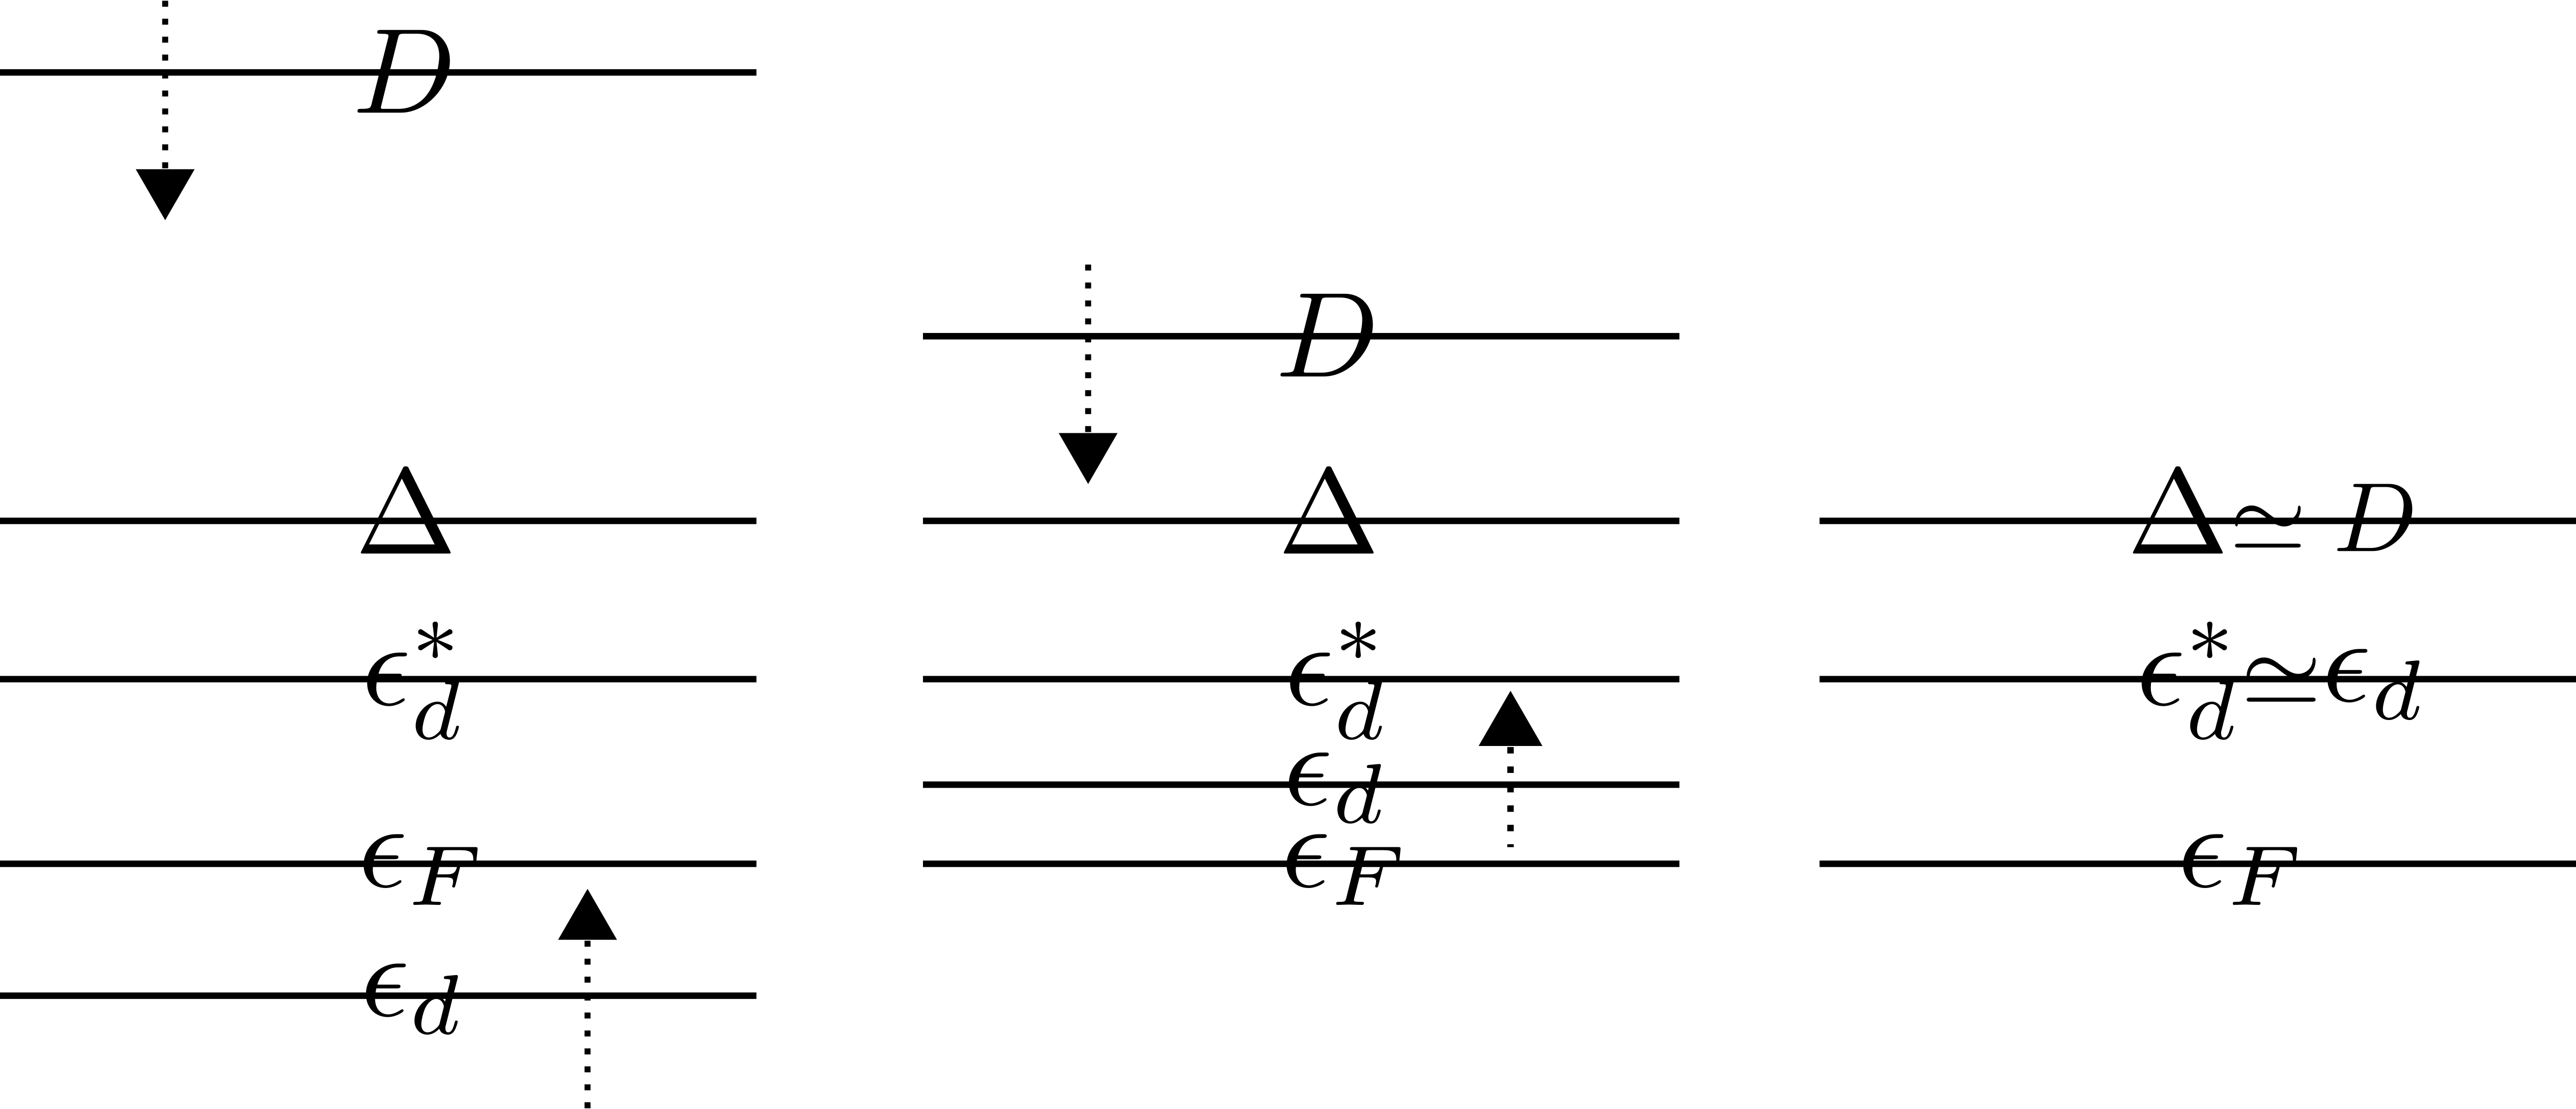
\includegraphics[scale=0.29]{mixed.png}\caption{Renormalization in energy levels when \il{|\epsilon_d^*| \lesssim \Delta}} \end{figure}
Since we have \il{|\epsilon_d^*| \lesssim \Delta}, as we renormalize, the decreasing cutoff will first match \il{\Delta} or \il{k_B T}, whichever is greater.
From eq.~\ref{mirai2}, we know that if \il{D} comes close to \il{\Delta}, our analysis will break down because we can no longer ignore that term.
Since that term represents the broadening of the impurity level, this same broadening can also be brought about by the thermal fluctuations which are of the scale \il{k_B T}.
This means that real valence fluctuations will now renormalize the potential \il{V_{kd}}.
Hence, our analysis will stop at \il{D = \text{max}\cc{\Delta, k_B T}}.
For the simpler situation in which \il{T = 0}, the renormalization will stop at \il{D = \Delta}.
From eq.~\ref{const}, putting \il{D = \Delta}, we get
\beq
\rr{\epsilon_d}_\text{MV} = \epsilon_d^*
\eeq
This is the renormalized impurity level in the mixed valence regime.
A characteristic feature of this regime is that the charge fluctuations can be thermally excited.
This can be seen as follows.
The probability of  a transition from, say, \il{\ket{n_d = 0}} to \il{\ket{n_d = 1}} is
\beq
\sim \fr{k_B T}{\epsilon_d}
\eeq
Assuming the thermal fluctuations are more or less of the order \il{\Delta}, for \il{\epsilon_d \gg \Delta}, this transition will not be possible.
However, in the mixed valence regime, because \il{\epsilon_d \sim \Delta}, these excitations do occur.
These fluctuations, as well as the ones from the hybridisation with the conduction band, are responsible for the mixing of the singly-occupied and null-occupied states.\\\\
The crossovers in the mixed valence regime are as follows.
Similar to the previous case, at high and intermediate temperatures, we have \il{n_d = 1} and \il{n_d = \fr{2}{3}} respectively.
However, while the triplet degeneracy lasted upto \il{T \sim T^*} in the previous case, here it continues up to \il{T \sim \Delta} because that is where the scaling breaks down.
That is, \il{T = \Delta} is the point where we can no longer ignore the renormalization in \il{V} and it begins to increase with scaling.
Beyond this point, the impurity occupation remains fractional and not much else can be said.
\begin{center}
\begin{minipage}{50pt}
\il{n_d = 1}\\\il{\chi T = \fr{1}{8}}\\\il{T\gg U}
\end{minipage}
\hspace*{20pt}\il{\Longrightarrow}\hspace*{20pt}
\begin{minipage}{50pt}
\il{n_d = \fr{2}{3}}\\\il{\chi T = \fr{1}{6}}\\\il{T\gg \Delta}
\end{minipage}
\hspace*{20pt}\il{\Longrightarrow}\hspace*{20pt}
\begin{minipage}{50pt}
	\il{n_d = \text{fractional}}\\\il{\chi T \propto T}\\\il{T\ll \Delta}
\end{minipage}
\end{center}
For \il{\epsilon_d^* \ll -\Delta}, the scaling will stop when the impurity level again goes out of the Fermi surface.
But this time, it goes out from below.
This again decouples the singly-occupied state from the conduction band and the scaling stops.
This happens at say \il{\wl D = -\wl {\epsilon_d} = \wl {T}}.
Since the singly-occupied impurity level is now well below \il{-D}, we have \il{\avg{n_d} = 1} and we are comfortably in the Kondo limit and the SWT and a consequent poor man's scaling can be performed, which will give eqs.~\ref{historia} through \ref{jean2}.
The resulf of the Schrieffer-Wolff transformation is a Hamiltonian that couples the impurity to the conduction electrons only through their spins; their is no charge fluctuation.
At high temperatures \il{T \gg T_K}, the impurity is essentially decoupled and we get a susceptibility of the form eq.~\ref{suscdeg}, but with a degeneracy of 2.
To go to lower temperatures, we can do a Poor Man's scaling which suggests that the Hamiltonian at \il{T\ll T_K} is one with a large coupling between the impurity and the conduction electrons.

\begin{center}
\begin{minipage}{50pt}
\il{n_d = 1}\\\il{\chi T = \fr{1}{8}}\\\il{T\gg U}
\end{minipage}
\hspace*{20pt}\il{\Longrightarrow}\hspace*{20pt}
\begin{minipage}{50pt}
\il{n_d = \fr{2}{3}}\\\il{\chi T = \fr{1}{6}}\\\il{T\gg \wl T}
\end{minipage}
\hspace*{20pt}\il{\Longrightarrow}\hspace*{20pt}
\begin{minipage}{50pt}
\il{n_d = 1}\\\il{\chi T= \fr{1}{4}}\\\il{T\ll \wl T}
\end{minipage}
\hspace*{20pt}\il{\Longrightarrow}\hspace*{20pt}
\begin{minipage}{50pt}
\il{n_d = 1}\\\il{\chi T \propto T}\\\il{T\ll \wl T_K}
\end{minipage}
\end{center}
\begin{figure}
	\centering 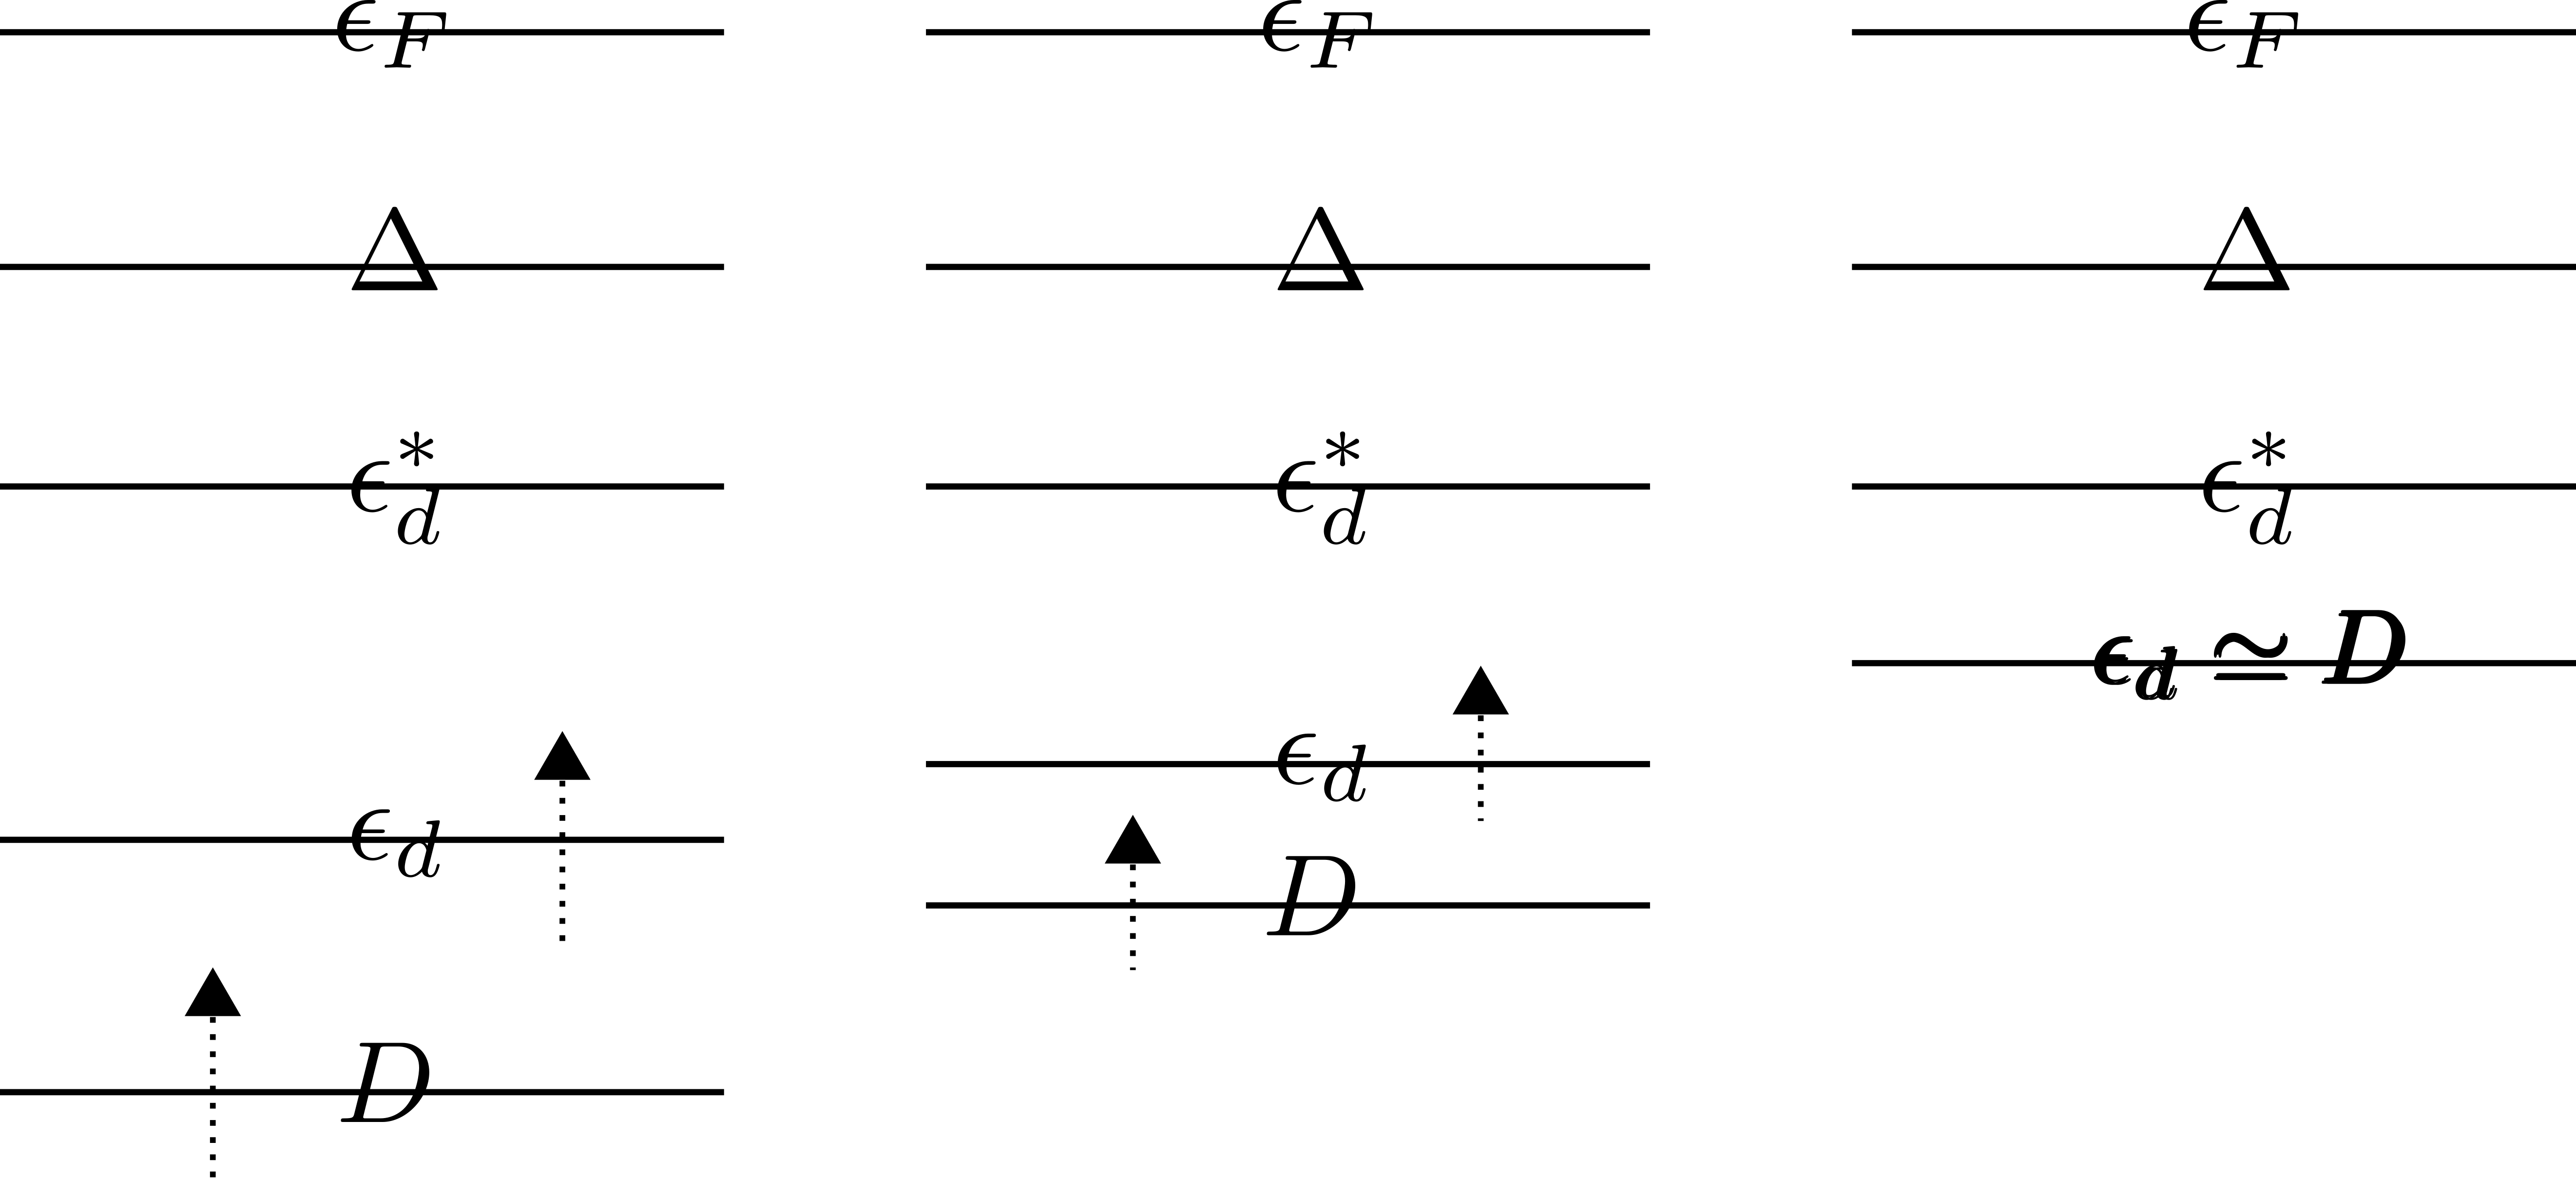
\includegraphics[scale=0.29]{empty.png}\caption{Renormalization in energy levels when \il{\epsilon_d^* \ll -\Delta}}
\end{figure}

\subsubsection*{Jefferson's calculation}
Jefferson did a slightly more rigorous calculation to obtain the scaling equation.
He divided the Hamiltonian into two parts
\beq
H = \sum_{k\sigma}\epsilon_{k\sigma} n_{k\sigma} + \epsilon_d n_d + \sum_{k\sigma} \rr{V^-_{kd}c^\dagger_{k\sigma}c_{d\sigma} + V^+_{kd}c^\dagger_{d\sigma}c_{k\sigma}} = H_0 + V
\eeq
Before scaling, \il{V^+ = V^- = V}.
The Schrödinger equation we want to solve is
\beq
H \psi = E \psi
\eeq
We know the eigenstates \il{\psi_0} of \il{H_0}.
They are the states \il{\{\ket{n_{k_i\sigma},n_{d\sigma^\prime}}\}}.
These states of course span the entire Hilbert space.
A subset of these states form the model subspace.
We call these states \il{\phi}.
For our case, that is the subspace with all conduction electrons inside \il{D - \delta D}.
The projection operator for this subspace is 
\beq
P = \sum \ket{\phi}\bra{\phi} =  \sum_{|k|<D-\delta D, \sigma=\pm 1, n_{d\sigma}=0,1} \ket{n_{k\sigma},n_{d\sigma^\prime}}
\eeq
Its orthogonal subspace has a projection operator
\beq
Q = 1 - P = \sum_{D-\delta D < |k| < D, \sigma=\pm 1, n_{d\sigma}=0,1} \ket{n_{k\sigma},n_{d\sigma^\prime}}
\eeq
If the dimension of model subspace if \il{d}, we can say that \il{P} takes \il{d} eigenstates \il{\psi} of the total Hamiltonian to \il{d} eigenstates in the model subspace:
\beq
P \{\psi\}_d = \{\phi\}
\eeq
This is of course true in the non-interacting limit.
There, the \il{\psi_0} are the exact eigenstates, and the action of \il{P} is basically
\beq
P \psi_0\bigg\vert_{|k|<D-\delta D} = \psi_0\bigg\vert_{|k|<D-\delta D}
\eeq
Now, as we turn on the interactions adiabatically, it is safe to assume that these \il{d} non-interacting eigenstates flow into \il{d} interacting eigenstates.
This means that we can define an inverse for the \il{P} operator which takes a non-interacting eigenstate from the model subspace into the interacting eigenstate:
\beq
\Omega \{\phi\} = \{\psi\}
\eeq
Since \il{\Omega} can only act on states in the model subspace, we define
\beq
\Omega \{\phi\}^\perp = 0
\eeq
This allows us to write
\begin{gather}
\Omega P \phi = \Omega \phi\\
\Omega P \phi^\perp = \Omega \times 0 = 0  = \Omega \phi^\perp
\end{gather}
In the first equation, I used \il{P \phi = \phi} because the projection of \il{\phi} into the model subspace is \il{\phi} itself.
Together these two identities give
\beq[hikki]
\Omega P = \Omega
\eeq
With these definitions, we now change the problem a bit.
We want to solve the Schrödinger equation only in the model subspace.
To this end we write the Schrödinger equation as
\beq
H \Omega \phi = E \Omega \Phi \\
\eeq
Since we want to write down an equation only in the model subspace, the equation should operate only on the \il{\phi}.
To remove the \il{\Omega} on the right side, operate on this equation with \il{P} from the left.
This gives
\beq
P H \Omega \phi = E P \Omega \phi = E \phi\\
\eeq
This is the effective Schrödinger equation in the model subspace.
The effective Hamiltonian for the model subspace is
\beq[yuigahama]
H_\text{eff} = PH\Omega  = PH_0 P + PV\Omega = P H_0 P + PV\Omega
\eeq
To solve for the \il{\Omega}, apply eq.~\ref{hikki} on the Schrödinger equation \il{(E - H_0)\psi =V \psi}:
\beq
\Omega V\psi = (E \Omega P - \Omega P H_0)\psi
\eeq
Now, since \il{P} is made up of the eigenstates of \il{H_0}, those two will commute: \il{\qq{H_0, P} = 0}.
The equation then becomes
\beq
\Omega V\psi = (E - \Omega H_0 P)\psi
\eeq
Subtracting the Schrödinger equation from the last equation gives
\beq
\rr{\Omega - 1} V\psi &= \rr{H_0 - \Omega H_0 P}\psi\\
\implies \rr{\Omega - 1} V \Omega \phi &= \rr{H_0 - \Omega H_0 P}\Omega \phi\\
\implies \rr{\Omega - 1} V \Omega \phi &= \rr{H_0 \Omega - \Omega H_0} \phi\\
\implies \rr{\Omega - 1} V \Omega &= \qq{H_0, \Omega}
\eeq
This is the main equation.
To make progress, we expand the operator \il{\Omega} in powers of the interaction \il{V}:
\beq
\Omega = \sum_n c_n V^n = \sum_n \Lambda_n
\eeq
The zeroth term in the main equation becomes
\beq
\qq{H_0, \Lambda_0} = 0 \implies \Lambda_0 = P
\eeq
The first order equation is
\beq
\qq{H_0, \Lambda_1} = \rr{\Lambda_0 - 1}V\Lambda_0 = \rr{P - 1}VP = -QVP
\eeq
The second order equation is
\beq
\qq{H_0, \Lambda_2} = -V\Lambda_1 + \Lambda_0 V \Lambda_1 + \Lambda_1 V \Lambda_0 = -QV\Lambda_1 + \Lambda_1 V P
\eeq
These equations are of the form \il{\qq{H_0, \Lambda_n} = A_n}, where \il{A_n} is an operator in terms of \il{\Lambda_{n-1}} and lower orders.
\begin{gather}
A_1 = -QVP\\
A_2 = -QV\Lambda_1 + \Lambda_1 V P
\end{gather}
Let \il{\ket{l}} and \il{\ket{h}} belong to the model subspace and its orthogonal subspace respectively.
Then, taking matrix element between \il{\bra{h}} and \il{\ket{l}} of the general form equation gives
\beq
\bra{h} A_n \ket{l} = \rr{E_h - E_l}\bra{h}\Lambda_n \ket{l} \implies \bra{h}\Lambda_n \ket{l} = \fr{\bra{h} A_n \ket{l}}{E_h - E_l}
\eeq
If we define an operator \il{S} by its action on a general operator A as
\beq
\bra{h}S A \ket{l} = \fr{\bra{h} A \ket{l}}{E_l - E_h}
\eeq
we can write the solution
\beq
\Lambda_n = -S(A_n)
\eeq
The expression of \il{SA} can be written as
\beq
SA &= \sum_{h,l}\ket{h}\bra{l} \fr{\bra{h}A\ket{l}}{E_l - E_H} \\
   &= \sum_{h,l}\fr{1}{E_l - E_h}\ket{h}\bra{h}A\ket{l}\bra{l}\\
   &= \sum_{l}\fr{1}{E_l - H_0}\rr{\sum_h \ket{h}\bra{h}}A\ket{l}\bra{l}\\
   &= \sum_l G_l A P_l
\eeq
where \il{P_l = \ket{l}\bra{l}} and \il{G_l = \fr{1}{E_l - H_0}Q}.\\\\
\il{S} has the property
\beq
\bra{h}S QA \ket{l} &= \fr{\bra{h}Q A \ket{l}}{E_l - E_h} = \fr{\bra{h}A \ket{l}}{E_l - E_h} = \bra{h}SA\ket{l} \\
\implies S(QA) &= S(A)
\eeq
The lowest order solutions are thus
\begin{gather}
	\Lambda_1 = S(QVP) = S(VP)\\
	\Lambda_2 = S(QV\Lambda_1) - S(\Lambda_1 V P) = S(VS(VP)) - S(S(VP)VP)
\end{gather}
We can now expand the effective Hamiltonian in powers of \il{V}.
From eq.~\ref{yuigahama}, the interacting part of the effective Hamiltonian becomes
\beq
H_\text{eff} - P H_0 P &= P V\Omega \\
		       &\approx PV(\Lambda_0 + \Lambda_1 + \Lambda_2)\\
				   &= PV\qq{P + S(VP) + S(VS(VP)) - S(S(VP)VP)}\\
				   &= PVP + PVS(VP) + PVS(VS(VP)) - PVS(S(VP)VP)
\eeq
Therefore,
\beq
H_\text{eff} = PHP + PVS(VP) + PVS(VS(VP)) - PVS(S(VP)VP)
\eeq
The first term is the obvious lowest approximation; you just project the entire Hamiltonian into the model subspace.
 The second term is
\beq
PVSVP = PV \sum_l G_l V P P_l = PV \sum_l G_l V P_l
\eeq
where I used \il{P P_l = \sum_{l^\prime} \ket{l^\prime}\bra{l^\prime} \ket{l}\bra{l} = \sum_{l^\prime}\ket{l^\prime}\bra{l^\prime}\delta_{ll^\prime} = P_l}.
The third term becomes
\beq
PVSVSVP  = PVSV \sum_l G_l V P_l = PV\sum_l S V G_l V P_l \\
= PV\sum_{l,l^\prime} G_{l^\prime} V G_l V P_lP_{l^\prime} = PV \sum_l  G_{l} V G_l V P_l
\eeq
The fourth term is
\beq
PVS(S(VP)VP) = PVS(\sum_l G_l VP P_l VP) = PV \sum_{l,l^\prime} G_{l^\prime} G_l VP_l VP P_{l^\prime} \\
= PV \sum_{l^\prime} G_{l^\prime} \rr{\sum_l G_l VP_l} V P_{l^\prime}
\eeq
The effective Hamiltonian up to third order in \il{V} is
\beq
H_\text{eff} = PH_0 P + PV \sum_l G_l V P_l + PV \sum_l  G_{l} V G_l V P_l \\
- PV \sum_{l,l^\prime} G_{l^\prime} G_l VP_l V P_{l^\prime}
\eeq
These results have been more or less general.
We now need to write these in terms of the creation and annihilation operators of our Hamiltonian.
The model subspace for our problem is the part of the conduction band up to \il{D - \delta D}.
Here on, \il{\sum} represent sum over the model subspace momenta and \il{\sum^\prime} represent sum over the remaining momenta.
To facilitate writing the effective Hamiltonian in terms of the creation and annihilation operators, we change the projection operators from the bra-ket representation to operator representation:
\begin{gather}
	\ket{k_1}\bra{k_2} = c^\dagger_{k_1}c_{k_2} \\
	P_k = \ket{k,n_{d\sigma}}\bra{k,n_{d\sigma}} = c^\dagger_{k}c_{k}c^\dagger_{d\sigma}c_{d\sigma} = n_{k\sigma}n_{d\sigma}
\end{gather}
The first term becomes
\beq
P H_0 P = \sum_{k\sigma} \epsilon_{k\sigma} n_{k\sigma} + \epsilon_d n_d + \sum_{k\sigma}\rr{V_{kd} c^\dagger_{k\sigma} c_{d\sigma} + \text{h.c.}}
\eeq
The second term involves two potential terms that scatter from the model subspace to the high energy subspace and then back to the model subspace.
Hence this term is 
\beq
PV \sum_l G_l V P_l  &= V \sum_{q\sigma}\rr{\fr{V_q}{\epsilon_d - \epsilon_q} c^\dagger_{q\sigma}c_{d\sigma} + \fr{V^*_q}{\epsilon_q - \epsilon_d} c^\dagger_{d\sigma}c_{q\sigma}}\\
		     &= {\sum_{q\sigma}}^+\fr{|V_q|^2 c^\dagger_{d\sigma}c_{q\sigma} c^\dagger_{q\sigma}c_{d\sigma}}{\epsilon_d - \epsilon_q} + {\sum_{q\sigma}}^-\fr{|V_q|^2c^\dagger_{q\sigma}c_{d\sigma}c^\dagger_{d\sigma}c_{q\sigma}}{\epsilon_q - \epsilon_d}\\
		     &= {\sum_{q\sigma}}^+\fr{|V_q|^2 n_{d\sigma}\rr{1-n_{q\sigma}}}{\epsilon_d - \epsilon_q} + {\sum_{q\sigma}}^-\fr{|V_q|^2n_{q\sigma}\rr{1-n_{d\sigma}}}{\epsilon_q - \epsilon_d}\\
\eeq
In the high energy subspaces, \il{n_q^+ = 1-n_q^- = 0}.
Therefore,
\beq
PV \sum_l G_l V P_l  &= {\sum_q}^+\fr{|V_q|^2 n_{d\sigma}}{\epsilon_d - \epsilon_q} + {\sum_q}^-\fr{|V_q|^2\rr{1-n_{d\sigma}}}{\epsilon_q - \epsilon_d} \\
		     &= n_d \rr{{\sum_q}^+\fr{|V_q|^2 }{\epsilon_d - \epsilon_q} + 2{\sum_q}^-\fr{|V_q|^2}{\epsilon_d - \epsilon_q}}\\
		     &= n_d \delta \epsilon_d
\eeq
The third term is zero in our case.
The part \il{G_l V G_l V} will do the following.

\beq
\ket{k,n_{d\sigma}} \ra \begin{cases} \ket{q_e,n_d=0} \ra \begin{cases} \ket{q_e,n_d=1}\\\ket{q_e,q^\prime_h,n_d = 1} \end{cases}
\\ 
\ket{q_h,n_d=1} \ra \begin{cases} \ket{q_h,q^\prime_e,n_d=0} \\ \ket{q_h,n_d=0} \end{cases}
\end{cases} 
\eeq
None of the four final states belong to the model subspace, so this term is zero.\\\\
The fourth term involves a first scattering between two model states, followed by a scattering to a high energy subspace and then a scattering back to the model subspace.
One way for going through such a process is
\beq
\ket{k,n_d = 0} \underbrace{\ra \ket{n_d=1} \ra}_{\Delta E = \epsilon_k - \epsilon_q} \ket{q_e,n_d = 0} \underbrace{\ra}_{\Delta E = \epsilon_q - \epsilon_d} \ket{k^\prime, n_d = 1}
\eeq
Another way is to start with \il{c_d} instead of \il{c^\dagger_d} 
\beq
\ket{n_{d\sigma} = 1} \underbrace{\ra \ket{k\sigma,n_d=0} \ra}_{\Delta E = \epsilon_k - \epsilon_q} \begin{cases} \ket{q_h\ua, n_{d\ua} = 1}\\ \ket{q_h\da, n_{d\da} = 1} \end{cases} \underbrace{\ra}_{\Delta E = \epsilon_q - \epsilon_d} \ket{n_d = 0}
\eeq
Combining the two processes gives

\beq
{\sum_{q}}^+\sum_{k\sigma} \fr{|V_q|^2c^\dagger_{d\sigma}c_{q\sigma}c^\dagger_{q\sigma}c_{d\sigma}c^\dagger_{d\sigma}c_{k\sigma}}{(\epsilon_q - \epsilon_d)(\epsilon_k - \epsilon_q)} + {\sum_{q\sigma^\prime}}^-\sum_{k\sigma} \fr{|V_q|^2c^\dagger_{q\sigma^\prime}c_{d\sigma^\prime}c^\dagger_{d\sigma^\prime}c_{q\sigma^\prime}c^\dagger_{k\sigma}c_{d\sigma}}{(\epsilon_q - \epsilon_d)(\epsilon_k - \epsilon_q)}\\
=\sum_{k\sigma}\rr{c^\dagger_{k\sigma}c_{d\sigma} \delta V^-_k + c^\dagger_{d\sigma}c_{k\sigma}\delta V^-_k}
\eeq
where
\beq
\delta V^+ = {\sum_q}^+ \fr{|V_q|^2}{(\epsilon_q - \epsilon_d)(\epsilon_k - \epsilon_q)}\\
\delta V^- = {\sum_q}^- 2\fr{|V_q|^2}{(\epsilon_q - \epsilon_d)(\epsilon_k - \epsilon_q)}
\eeq
The total Hamiltonian can be written in the form
\beq
H_\text{eff} = \sum_{k\sigma}\epsilon_{k\sigma} n_{k\sigma} + &\rr{\epsilon_d + \delta \epsilon_d}n_d \\
												     + &\sum_{k\sigma}\cc{\rr{V^-_k + \delta V^-_k} c^\dagger_{k\sigma}c_{d\sigma} + \rr{V^+_k + \delta V^+_k} c^\dagger_{d\sigma}c_{k\sigma}}
\eeq
We now evaluate the changes:
\beq
\delta \epsilon_d &= \rr{{\sum_q}^+\fr{|V_q|^2 }{\epsilon_d - \epsilon_q} + 2{\sum_q}^-\fr{|V_q|^2}{\epsilon_d - \epsilon_q}} \\
&\approx |V|^2 \rho |\delta D| \rr{\fr{1}{\epsilon_d - D} + \fr{2}{\epsilon_d + D}}\\
&=|V|^2 \rho |\delta D|\fr{D - 3\epsilon_d}{D^2 - \epsilon_d^2}
\eeq
I used the approximation
\beq
\sum_{q=D-\delta D}^D f(q) = \int_{D- \delta D}^D dE \rho(E) f(E) \approx \rho f(D) \delta D
\eeq
Also,
\beq
\delta V_k^+ &= {\sum_q}^+ \fr{|V_q|^2}{(\epsilon_q - \epsilon_d)(\epsilon_k - \epsilon_q)}\\
	       &\approx |V|^2 \rho |\delta D|\fr{1}{(D - \epsilon_d)(\epsilon_k - D)}\\
\delta V_k^- &= 2{\sum_q}^- \fr{|V_q|^2}{(\epsilon_q - \epsilon_d)(\epsilon_k - \epsilon_q)}\\
	       &\approx -|V|^2 \rho |\delta D|\fr{2}{(D + \epsilon_d)(\epsilon_k + D)}
\eeq
We now make the following assumptions:
\begin{itemize}
	\item \il{k} is close to the Fermi level (\il{\epsilon_k \approx 0})
	\item Because \il{k} is close to the Fermi surface, we assume the potential is independent of momenta: \il{V_k^+ \equiv v^+, V^-_k \equiv v^-}
	\item Since we truncated at third order, we need \il{D - |\epsilon_d| \gg v^\pm}.
This gives us \il{D \gg |\epsilon_d|}.
\end{itemize}
With these assumptions, we get the scaling equations similar to the ones obtained previously.

\section{URG Method}\label{section2}
\subsection{Formalism}\label{urgform}
This section is adapted from ref.\cite{holography1}.
We are given a Hamiltonian \il{\ham} which is not completely diagonal in the occupation number basis of the electrons, \il{\hat n_k}: \il{\qq{\ham,n_k} \neq 0}. \(k\) labels any set of quantum numbers depending on the system. For spin-less Fermions it can be the momentum of the particle, while for spin-full Fermions it can be the set of momentum and spin. There are terms that scatter electrons from one quantum number \(k\) to another quantum number \(k^\prime\).
\pb To begin, we choose an electron with a particular value of quantum numbers, which we label \(q\). It might be the electron with the highest momentum or that at the first lattice site. The goal is to obtain a unitary transformation \il{U_q} that diagonalizes this Hamiltonian in this particular electron's basis. Once this is done, we can choose another electron (the next highest momentum or the second lattice site) and diagonalize the Hamiltonian in this electron's basis.
\pb \(U_q\) is defined by
\beq
\tilde \ham = U_q \ham U^\dagger_q \text{   such that  } \qq{\tilde \ham,n_q} = 0
\eeq
Another way to express the above problem is that, with the original Hamiltonian \il{\ham}, the diagonal terms are not zero:
\beq
n_q \ham(1-n_q) \neq 0
\eeq
so we want to find a rotated Hamiltonian \il{\tilde \ham = U_q \ham U_q^\dagger} such that the off-diagonal term is zero:
\beq[solve]
n_q \tilde \ham(1-n_q) =0
\eeq
To make progress, we write the Hamiltonian \il{\ham} as
\beq[ham]
\ham = \ham^D + \ham^I + \ham^i 
\eeq
\begin{minipage}{310pt}
	\il{\ham^D} is the diagonal part of the Hamiltonian, something of the form \il{\sum_k \epsilon_k n_k}.
It also has the self energies that might arise from certain interactions.
For example, if we have an interaction term of the form \(J \sum_{k_1,k_2}c^\dagger_{k_1}c_{k_2}\), the term where both momenta are equal gives a diagonal term \(J c^\dagger_{k_1}c_{k_1}\).
Such terms are also included in \(\ham^D\).
\pb \il{\ham^I} is the interaction between the current degree of freedom \il{q} and the remaining degrees of freedom \(k\).
It will consist of terms like \il{c^\dagger_q c_k} or \il{c^\dagger_k c_q} that scatter between the current degree of freedom and the other degrees of freedom.
\end{minipage}
\hspace*{20pt}\begin{minipage}{200pt}
\begin{center}
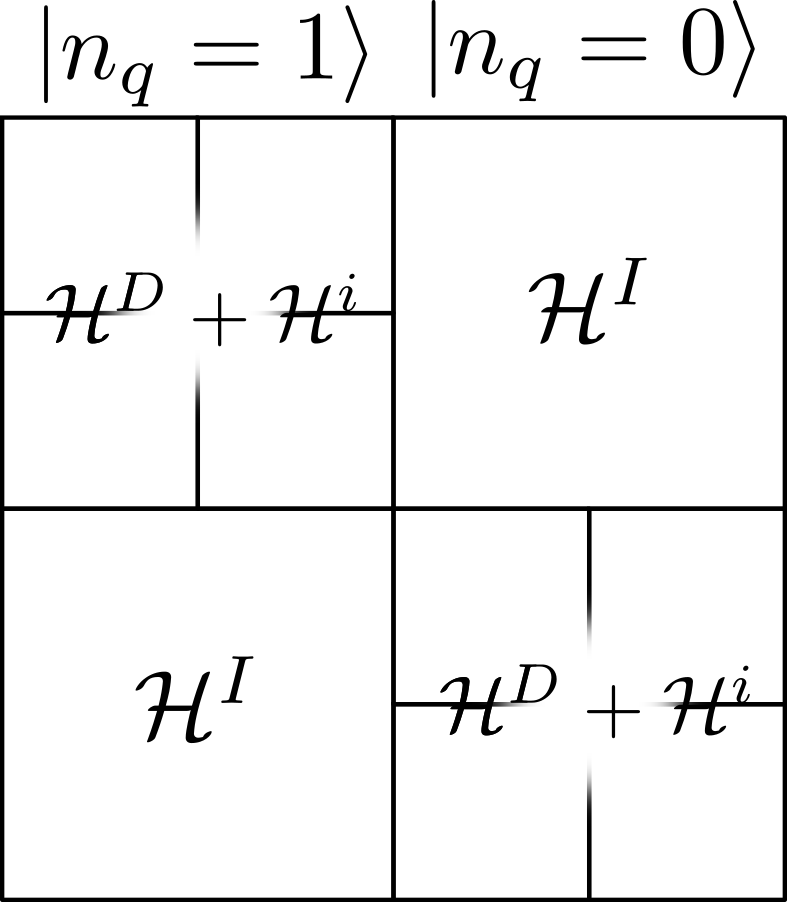
\includegraphics[scale=0.7]{ham.png}
\captionof{figure}{Decomposition of Hamiltonian}
\end{center}
\end{minipage}
\pb The third term \il{\ham^i} has interactions between the remaining degrees of freedom.
This term will also be diagonal in \il{n_k} because it doesn't involve scattering either from or into \il{q} states.
It will involve terms like \il{c^\dagger_{k_1}c_{k_2}}.
\pb Let \(\cc{\ket{\Psi}_q}\) be the set of states in which \(\ham\) assumes a diagonal form in the space of \(q\). This diagonal form is of course also what we get when we apply the unitary transformation \(U_q\) on the Hamiltonian.
\beq[tanjiro]
\ham \ket{\Psi}_q = \tilde \ham \ket{\Psi}_q
\eeq
\comm{
	To find the form for \il{U_k}, we define a few things.
First,
\beq
P_k = U_k^\dagger n_k U_k
\eeq
To get a feel for what \il{P_k} is, note that
\beq
\qq{\ham, P_k} = \qq{U^\dagger_k U_k \ham, U_k^\dagger n_k U_k} = U_k^\dagger \qq{\wl \ham, n_k}U_k = 0
\eeq
\il{P_k} is hence those degrees of freedom in which the given Hamiltonian \il{\ham} is diagonal.
Hence it is natural that they are obtained by rotating the \il{n_k}.
If we were to go to the eigenbasis of \ham, the form for \il{\wl \ham} will be 
\beq
\begin{pmatrix} E_1 & \\ & E_2 \end{pmatrix}
\eeq
while the form for \il{P_k} will be
\beq
\begin{pmatrix} 1 & 0  \\ 0 & 0\end{pmatrix}
\eeq
It is obvious that
\beq
P_k^2 = P_k
\eeq
Another thing that we will define is
\beq
\ol \ham  = P_k \ham P_k
\eeq
\il{\ol \ham} is a matrix that, in the eigenbasis of \ham, has only the upper diagonal block of \il{\ham}.
 That is, you first form a matrix by keeping only the upper diagonal block of \il{\wl \ham} and then rotating to the basis of \il{n_k}.
Finally, let \il{\psi} be a wavefunction such that
\beq
P\psi = \psi
\eeq
This means that \il{\psi} is an eigenvector of \il{P_k} and hence also of \il{\ham} since \il{P_k} and \il{\ham} commute.
\\\\
Combining \il{P_k \ham = \ham P_k} and the idempotence of \il{P_k} gives
\beq
\ham P_k = P_k \ham = P_k \ham P_k = \ol\ham
\eeq
Operating this equation on \il{\psi} gives
\beq[tanjiro]
\ham \psi = \ol \ham \psi
\eeq
}
This is the equation we will use to find \il{U_q}.
But first we will write \il{\psi} in the following fashion:
\beq
\ket{\Psi} = a_1 \ket{1,\Psi_1} + a_0\ket{0,\Psi_0}
\eeq
In the kets \(\ket{1,\Psi_1}\) and \(\ket{0,\Psi_0}\), the first entry (\(0/1\)) signifies whether the degree of freedom \il{q} is occupied or not, and the second entry is the wavefunction of the remaining degrees of freedom.
This is just a resolution of the total wavefunction in the two-dimensional Hilbert space of \il{q}.
\comm{
The Hamiltonian \il{\ol\ham} can also be decomposed in a similar form.
Note however that since it is already diagonal in \il{n_k}, it won't have any scattering in \il{k}, and hence won't have a term like \il{\ham^I}.
\beq
\ol \ham = \ol \ham^D + \ol \ham^i
\eeq}
Substituting the decomposition of \il{\ket{\Psi}} and \(\ham\) into eq.~\ref{tanjiro} gives
\beq[zenitsu]
\tilde \ham \rr{a_1\ket{1,\Psi_1} + a_0\ket{0,\Psi_0}} = \qq{\ham^D  + \ham^I + \ham^i }\rr{a_1 \ket{1,\Psi_1} + a_0\ket{0,\Psi_0}}
\eeq
To get expressions from this, note that on the left hand side, \il{\tilde \ham} does not scatter \il{q}, so it will not change the left entry in the kets; it can only change the right entries.
Similarly, on the right hand side, \il{\ham^D} and \il{\ham^i} will not change the occupation of the \il{k} degree of freedom.
\il{\ham^I} however \it{will} change it.
Matching the states with \il{\ket{0}} gives
\beq
\tilde \ham a_0\ket{0,\Psi_0} = \rr{\ham^D + \ham^i}a_0\ket{0,\Psi_0} + \ham^Ia_1\ket{1,\Psi_1}
\eeq
We can simplify this equation by noting that
\begin{gather}
\ham^D = \text{ Tr} \qq{\ham^D \hat n_q}\hat n_q + \text{ Tr} \qq{\ham^D (1 - \hat n_q)}(1-\hat n_q)\\
 \implies  \ham^D \ket{0,\psi_0} = \text{ Tr} \qq{\ham^D (1 - \hat n_q)}(1-\hat n_q)\ket{0,\psi_0}
\end{gather}
and
\begin{gather}
 \ham^I = \text{ Tr} \qq{c^\dagger_q \ham } c_q + c^\dagger_q \text{ Tr} \qq{\ham c_q}
 \implies \ham^I\ket{1,\psi_1} = \text{ Tr} \qq{c^\dagger_q \ham } c_q \ket{1,\psi_1}
\end{gather}
Substituting these in the equation gives
\begin{gather}
\tilde \ham a_0\ket{0,\Psi_0} = \cc{\text{ Tr} \qq{\ham^D (1 - \hat n_q)}(1-\hat n_q) + \ham^i}a_0\ket{0,\Psi_0}
+ \text{ Tr} \qq{c^\dagger_q \ham } c_q a_1\ket{1,\Psi_1}\\
\implies \cc{\tilde\ham - \ham^i - \text{ Tr} \qq{\ham^D (1 - \hat n_q)}(1-\hat n_q)} a_0 \ket{0,\Psi_0}
= \text{ Tr} \qq{c^\dagger_q \ham } c_q a_1\ket{1,\Psi_1}
\end{gather}
Defining \il{\hat \omega = \tilde\ham - \ham^i}, we get the result
\beq
a_0 \ket{0,\Psi_0} = \qq{\hat \omega - \text{ Tr} \qq{\ham^D (1 - \hat n_q)}(1-\hat n_q)}^{-1}\text{ Tr} \qq{c^\dagger_q \ham } c_q a_1\ket{1,\Psi_1}
\eeq
We define 
\beq[etadef]
\eta_q \equiv \fr{1}{\hat \omega - \text{ Tr} \qq{\ham^D (1 - \hat n_q)}(1-\hat n_q)}\text{ Tr} \qq{c^\dagger_q \ham } c_q
\eeq
which gives the equation a compact form
\beq
a_0 \ket{0,\Psi_0} = \eta_q a_1\ket{1,\Psi_1}
\eeq
The equation obtained by matching the states \il{\ket{1}} is
\beq
a_1 \ol \ham \ket{1,\Psi_1} &= \rr{\ham^D + \ham^i}a_1\ket{1,\Psi_1} + \ham^I a_0\ket{0,\Psi_0}\\
			    &= \rr{\text{ Tr }\qq{\ham^D \hat n_q}\hat n_q + \ham^i}a_1\ket{1,\Psi_1} + c^\dagger_q \text{ Tr }\qq{\ham c_q}a_0\ket{0,\Psi_0}\\
\implies a_1 \ket{\Psi_1} &= \rr{\ol\ham - \ham^i - \text{ Tr }\qq{\ham^D \hat n_q}\hat n_q }^{-1} c^\dagger_q \text{ Tr }\qq{\ham c_q}a_0\ket{0,\Psi_0}\\
			  &=\mu_q a_0\ket{0,\Psi_0}
\eeq
where 
\beq[etadagdef]
\mu_q = \fr{1}{\hat \omega - \text{ Tr} \qq{\ham^D \hat n_q}\hat n_q} c_q^\dagger \text{ Tr}\qq{ \ham c_q}
\eeq
We thus get the following two equations:
\begin{gather}
	a_0 \ket{0,\Psi_0} = \eta_q a_1\ket{1,\Psi_1}\label{eta}\\
	a_1 \ket{1,\Psi_1} = \mu_q a_0\ket{0,\Psi_0}\label{etad}
\end{gather}
Combining eqs.~\ref{eta} and \ref{etad}, we get
\beq
a_0 \ket{0,\Psi_0} = \eta_q a_1\ket{1,\Psi_1} = \eta_q \mu_q a_0 \ket{0,\Psi_0}
\eeq
Combining this with the fact that \il{\mu_q} should have a \il{c^\dagger_q} and hence should give \il{\mu_q \ket{1,\Psi_1}}, we get
\beq
\eta_q \mu_q = 1 - \hat n_q
\eeq
Similarly, combining the equations the other way round gives
\beq[prod]
\mu_q \eta_q = \hat n_q
\eeq
As a consequence,
\beq
 \cc{\eta_q,\mu_q} &= 1\\
 \qq{\eta_q,\mu_q} &= 1 - 2\hat n_q\\
\eeq
Other properties include
\begin{gather}
\eta_q^2 = \rr{\mu_q}^2 = 0\\
\hat n_q \eta_q = (1-\hat n_q)\mu_q = 0\\
\eta_q \hat n_q=\eta_q\\
\mu_q(1-\hat n_q) = \mu_q
\end{gather}
We now need to find the unitary operation \il{U_q} that disentangles the state \il{\ket{1,\Psi_1}} from the state \il{\ket{\Psi}}.
For the sake of unitarity, we restrict \(\mu_q = \eta^\dagger_q\). This restriction is transferred to the values of \(\hat \omega\).
Using eq.~\ref{eta},
\beq
\ket{\Psi} = a_1\ket{1,\Psi_1} + a_0\ket{0,\Psi_0}  = a_1\ket{1,\Psi_1} +  \eta_q a_1\ket{1,\Psi_1} = \rr{1+\eta_q}\ket{1,\Psi_1}
\eeq
Since \(\eta^2 = 0\), we can write \(1+\eta_q = e^{\eta_q}\). \(S \equiv e^{\eta_q}\) constitutes a similarity transformation. It is shown in ref.~\cite{suzuki} that corresponding to a similarity transformation \(e^\omega\),there exists a unitary transformation \(e^G\) where
\beq
G = \tanh^{-1}\rr{\omega - \omega^\dagger}
\eeq
Applying that to the problem at hand gives
\beq
 U^\dagger &= \ex{\tanh^{-1}\rr{\eta - \eta^\dagger}}\\
	   &= \frac{1 + \eta - \eta^\dagger}{1 + \cc{\eta,\eta^\dagger}}\\
	   &= \fr{1}{\sqrt 2}\rr{1 + \eta - \eta^\dagger}
\eeq
The unitary operator that transforms the entangled eigenstate \il{\ket{\Psi}} to the eigenstate with good quantum number \il{n_q}, \il{\ket{1,\Psi_1}} is thus
\beq
U_q = \fr{1}{\sqrt 2}\rr{1 + \eta_q^\dagger - \eta_q}
\eeq
The form of the rotated Hamiltonian can now be written down.
\beq[roth]
 \wl\ham &= U_q \ham U_q^\dagger\\
	 &= \hf\rr{1+\eta_q^\dagger - \eta_q}\ham\rr{1 + \eta_q - \eta^\dagger_q}\\
				&= \hf\rr{1+\eta_q^\dagger - \eta_q}\rr{\ham + \ham\eta - \ham\eta_q^\dagger}\\
				&=\hf\rr{\ham+ \ham\eta - \ham\eta_q^\dagger + \eta_q^\dagger \ham + \eta_q^\dagger\ham\eta_q - \eta_q^\dagger \ham\eta_q^\dagger - \eta_q\ham - \eta_q \ham \eta_q + \eta_q \ham \eta_q^\dagger}\\
&=\hf\rr{\ham^D + \ham^i + \ham^I + \ham\eta - \ham\eta_q^\dagger + \eta_q^\dagger \ham + \eta_q^\dagger\ham\eta_q - \eta_q^\dagger \ham\eta_q^\dagger - \eta_q\ham - \eta_q \ham \eta_q + \eta_q \ham \eta_q^\dagger}\\
&=\hf\rr{\ham^D + \ham^i + \ham^I + \qq{\eta^\dagger_q - \eta,\ham} + \eta_q^\dagger\ham\eta_q - \eta_q^\dagger \ham\eta_q^\dagger - \eta_q \ham \eta_q + \eta_q \ham \eta_q^\dagger}\\
\eeq
In the last step I split \il{\ham} using eq.~\ref{ham}.
For reasons that will become apparent later, we will split the terms into two groups:
\beq
 \tilde \ham &= \hf\rr{\underbrace{\ham^D + \ham^i + \qq{\eta^\dagger_q - \eta,\ham} + \eta_q^\dagger\ham\eta_q + \eta_q \ham \eta_q^\dagger}_\text{group 1} + \overbrace{\ham^I - \eta_q^\dagger \ham\eta_q^\dagger - \eta_q \ham \eta_q}^\text{group 2}}\\
\eeq
Group 2 consists of purely off-diagonal terms; they amount to 0. To see how, note that terms that have two \il{\eta_k} or two \il{\eta_q^\dagger} can only be nonzero if the intervening \il{\ham} has a creation or destruction operator.
We resolve the Hamiltonian in the basis of \il{q} in the following form:
\beq[hisoka]
 \ham &= \text{Tr}\qq{\ham \hat n_q}\hat n_q + \text{Tr}\qq{\ham \rr{1 - \hat n_q}}\rr{1 - \hat n_q} + c_q^\dagger \text{Tr}\qq{\ham c_q} + \text{Tr}\qq{c_q^\dagger \ham}c_q\\
      &=H_e \hat n_q + H_h (1-\hat n_q) + c^\dagger_q T + T^\dagger c_q
\eeq
Using this form, we can write
\beq[beats]
\eta_q \ham \eta_q = \eta_q c_q^\dagger  T \eta_q
\eeq
and
\beq[tora]
\eta_q^\dagger \ham\eta_q^\dagger = \eta_q^\dagger T^\dagger c_q \eta_q^\dagger
\eeq
We can also write the off-diagonal part as
\beq
\ham^I = c^\dagger_q T + T^\dagger c_q
\eeq
Group 2 becomes
\beq
\text{group 2} = c^\dagger_q T + T^\dagger c_q - \eta_q^\dagger T^\dagger c_q \eta_q^\dagger - \eta_q c_q^\dagger  T \eta_q
\eeq
To simplify this, we use the definition of \(\eta^\dagger_q\), eq.~\ref{etadagdef}, to write \(\eta_q\):
\beq
\eta_q = \rr{\eta_q^\dagger}^\dagger = \text{ Tr}\qq{ c^\dagger_q\ham }c_q\fr{1}{\hat \omega - \text{ Tr} \qq{\ham^D \hat n_q}\hat n_q} = T^\dagger c_q \fr{1}{\hat \omega - H_e \hat n_q}
\eeq
Using this, we can write
\beq
 \eta_q c_q^\dagger  T \eta_q &= T^\dagger c_q \fr{1}{\hat \omega - H_e \hat n_q}c_q^\dagger  T \eta_q\\
			      &= T^\dagger c_q \rr{\fr{1}{\hat \omega - H_e \hat n_q}c_q^\dagger  T} \eta_q\\
			      &= T^\dagger c_q \eta_q^\dagger\eta_q &&\qq{\text{eq.~\ref{etadagdef}}}\\
			      &= T^\dagger c_q \hat n_q &&\qq{\text{eq.~\ref{prod}}}
\eeq
which gives
\beq[id1]
 \eta_q c_q^\dagger  T \eta_q  &= T^\dagger c_q 
\eeq
Similarly, we can express \(\eta^\dagger_q\) by taking Hermitian conjugate of \(\eta_q\):
\beq
\eta^\dagger_q = \fr{1}{\hat \omega - H_h \rr{1 - \hat n_q}}T^\dagger c_q 
\eeq
which gives
\beq[id2]
\eta_q^\dagger T^\dagger c_q \eta_q^\dagger = c_q^\dagger T
\eeq
Substituting the expressions \ref{id1} and \ref{id2}, we get \(\text{group 2}=0\).
Substituting this in the rotated Hamiltonian gives
\beq
\wl \ham = \hf\rr{\ham^D + \ham^i + \ham\eta - \ham\eta_q^\dagger + \eta_q^\dagger \ham + \eta_q^\dagger\ham\eta_q - \eta_q\ham  + \eta_q \ham \eta_q^\dagger}
\eeq
To simplify the last 6 terms, we note the following:
\begin{gather}
 \eta_q^\dagger = \fr{1}{\omega - H_e \hat n_q}c^\dagger_q T,\;\;\;\;\;\;\; \eta_q = \fr{1}{\omega - H_h (1-\hat n_q)}T^\dagger c_q
 \end{gather}
 Then,
 \beq
 \implies& \fr{1}{\omega - H_e \hat n_q}c^\dagger_q T= c^\dagger_qT\fr{1}{\omega - H_h (1-\hat n_q)}\\
 \implies& c_q^\dagger T H_h(1-\hat n_q) = H_e \hat n_q c_q^\dagger T\\
 \implies& \fr{1}{\omega - H_e \hat n_q}c_q^\dagger T H_h(1-\hat n_q) = \fr{1}{\omega - H_e \hat n_q}H_e \hat n_q c_q^\dagger T\\
 \implies& \eta_q^\dagger H_h(1-\hat n_q) = H_e \hat n_q \fr{1}{\omega - H_e \hat n_q}c_q^\dagger T\\
 \implies& \eta_q^\dagger H_h(1-\hat n_q) = H_e \hat n_q \eta_q^\dagger\\
 \implies& \eta_q^\dagger H_h = H_e \hat \eta_q^\dagger\label{iden}
\eeq
Using this identity and its conjugate (\il{\eta_q H_e = H_h \hat \eta_q}), the expression for \il{\eta_q H \eta_q^\dagger} can be simplified:
\beq
 \eta_q \ham \eta_q^\dagger &= \eta_q H_e \hat n_q \eta_q^\dagger\\
			    &= H_h \eta_q \eta_q^\dagger\\
			    &= H_h (1-\hat n_q)
\eeq
Similarly,
\beq
 \eta_q^\dagger  \ham \eta_q&= \eta_q^\dagger  H_h \eta_q\\
			    & = H_e \eta_q^\dagger \eta_q\\
			    &= H_e \hat n_q
\eeq
Also, 
\beq
\ham\eta - \ham\eta_q^\dagger + \eta_q^\dagger \ham - \eta_q\ham = \rr{\eta^\dagger_q H_h - H_e \eta_q^\dagger} + \rr{H_h \eta - \eta H_e} + \eta_q^\dagger T^\dagger c_q - \eta_q c^\dagger_q T + \\
c_q^\dagger T \eta_q - T^\dagger c_q \eta_q^\dagger
\eeq
By virtue of eq.~\ref{iden} and its conjugate, the first two terms will vanish.
\beq[link]
\ham\eta - \ham\eta_q^\dagger + \eta_q^\dagger \ham - \eta_q\ham = \eta_q^\dagger T^\dagger c_q - \eta_q c^\dagger_q T + c_q^\dagger T \eta_q - T^\dagger c_q \eta_q^\dagger
\eeq
From eqs.~\ref{id1} and \ref{id2},
\begin{gather}
\eta_q^\dagger T ^\dagger c_q = \eta_q^\dagger \eta_q c_q^\dagger T \eta_q = \hat n_q c_q^\dagger T\eta_q = c_q^\dagger T\eta_q\\
T ^\dagger c_q \eta_q^\dagger = \eta_q c_q^\dagger T \eta_q \eta_q^\dagger = \eta_q c_q^\dagger T \rr{1-\hat n_q} = \eta_q c_q^\dagger T\\
\end{gather}
Eq.~\ref{link} becomes
\beq
 \ham\eta - \ham\eta_q^\dagger + \eta_q^\dagger \ham - \eta_q\ham &= c_q^\dagger T\eta_q - \eta_q c^\dagger_q T + c_q^\dagger T \eta_q - \eta_q c_q^\dagger T
								     &=2\qq{c_q^\dagger T,\eta_q}
\eeq
Putting it all together,
\beq
 \wl \ham &= \hf\rr{\ham^D + \ham^i + \ham\eta - \ham\eta_q^\dagger + \eta_q^\dagger \ham + \eta_q^\dagger\ham\eta_q - \eta_q\ham  + \eta_q \ham \eta_q^\dagger}\\
	  &=\hf\rr{\ham^D + \ham^i} + \qq{c_q^\dagger T,\eta_q} + \hf\qq{H_e \hat n_q + H_h(1-\hat n_q)}
\eeq
One further simplification is possible.
The last two terms constitute the total diagonal part of the Hamiltonian, but so do the first two terms:
\beq
\ham^D + \ham^i = H_e \hat n_q + H_h\rr{1-\hat n_q}
\eeq
Hence,
\beq
 \wl \ham &= \hf\rr{\ham^D + \ham^i + \ham\eta - \ham\eta_q^\dagger + \eta_q^\dagger \ham + \eta_q^\dagger\ham\eta_q - \eta_q\ham  + \eta_q \ham \eta_q^\dagger}\\
	  &=H_e \hat n_q + H_h(1-\hat n_q) + \qq{c_q^\dagger T,\eta_q}\\
	  &=\text{Tr}\qq{\ham\hat n_q}\hat n_q + \text{Tr}\qq{\ham\hat(1- n_q)}(1-\hat n_q) + \qq{c_q^\dagger \text{Tr}\rr{\ham c_q},\eta_q}
\eeq
The two terms at the front can be written in a slightly different fashion.
\beq
 \text{Tr}\qq{\ham\hat n_q}\hat n_q + \text{Tr}\qq{\ham(1- \hat n_q)}(1-\hat n_q) &= \text{Tr}\qq{\ham\hat n_q}\hat n_q + \text{Tr}\qq{\ham(\hat n_q -1)}(\hat n_q -1)\\
										  &=\text{Tr}\qq{\ham\hat n_q}\hat n_q + \text{Tr}\qq{\ham(\hat n_q -1)}n_q -\text{Tr}\qq{\ham\hat(n_q -1)}\\
										  &=\text{Tr}\qq{\ham\rr{2\hat n_q - 1}}\hat n_q -\text{Tr}\qq{\ham(\hat n_q -1)}\\
										  &=\text{Tr}\qq{\ham\rr{\hat n_q - \hf}}2\hat n_q -\text{Tr}\qq{\ham(\hat n_q -\hf)} + \hf\text{Tr}\qq{\ham} \\
										  &= \text{Tr}\qq{\ham\rr{\hat n_q - \hf}}\rr{2\hat n_q - 1} + \hf\text{Tr}\qq{\ham}\\
										  &=\text{Tr}\qq{\ham\tau_q}2\tau_q + \hf\text{Tr}\qq{\ham}\\
\eeq
The last term can be written as:
\beq
 \qq{c_q^\dagger \text{Tr}\rr{\ham c_q},\eta_q} &= c_q^\dagger \text{Tr}\rr{\ham c_q}\eta_q - \eta_qc_q^\dagger \text{Tr}\rr{\ham c_q}\\
						&=\rr{2\hat n_q - 1}c_q^\dagger \text{Tr}\rr{\ham c_q}\eta_q - \rr{1-2\hat n_q}\eta_qc_q^\dagger \text{Tr}\rr{\ham c_q}
\eeq
I used \il{\hat n_q c^\dagger_q = c^\dagger_q} and \il{\hat n_q \eta_q = 0}.
Then,
\beq
 \qq{c_q^\dagger \text{Tr}\rr{\ham c_q},\eta_q} = 2\tau_q \cc{c_q^\dagger \text{Tr}\rr{\ham c_q},\eta_q}
\eeq
The final form of the rotated Hamiltonian is
\beq[final2]
\wl \ham = U_q \ham U_q^\dagger =  \text{Tr}\qq{\ham\hat n_q}\hat n_q + \text{Tr}\qq{\ham(1- \hat n_q)}(1-\hat n_q) + 2\tau_q \cc{c_q^\dagger \text{Tr}\rr{\ham c_q},\eta_q}
\eeq
To check that this indeed commutes with \il{\hat n_q},
\beq
 \qq{\wl \ham, \hat n_q} &= \qq{\qq{c_q^\dagger T,\eta_q},\hat n_q}\\
			 &=\qq{c_q^\dagger T \eta_q,\hat n_q} - \qq{\eta_q c_q^\dagger T,\hat n_q}\\
			 &=c^\dagger_q T \eta_q \hat n_q - \hat n_qc^\dagger_q T \eta_q &&\qq{\text{2\uu{nd} [ .
] is 0, }\because c_q^\dagger \hat n_q = \hat n_q \eta_q=0}\\
			 &=c_q^\dagger T \eta_q - c_q^\dagger T \eta_q\\
			 &=0
\eeq
Within the URG, it is a prescription that the fixed point is reached when the denominator of the RG equation vanishes. This is equivalent to the condition:
\begin{gather*}
\hat \omega - H_e \hat n = 0\\
\implies \omega_e = H_e
\end{gather*}
or 
\begin{gather*}
\hat \omega - H_h\rr{1 - \hat n} = 0\\
\implies \omega_h = H_h
\end{gather*}
In either case, we see that the eigenvalue of \(\hat \omega\) matches the eigenvalue of one of the blocks. This also leads to the vanishing of the off-diagonal block. To see how,
\beq
\eta^\dagger \eta \ket{1,\Psi_1} &= \ket{1,\Psi_1} &&\qq{\eta^\dagger \eta = \hat n}\\
\implies \fr{1}{\hat \omega - \hat H_e}c^\dagger T \eta &= \ket{1,\Psi_1} \\
\implies c^\dagger T \eta &= \rr{\hat \omega - \hat H_e}\ket{1,\Psi_1} \\
&= \rr{\omega_e - H_e}\ket{1,\Psi_1}\\
\eeq
If \(\omega_e = H_e\), we will have \(c^\dagger T = 0\). This implies \(T^\dagger c = 0\) and hence \(\ham^I = 0\).
\subsection{Prescription}
Given a Hamiltonian
\beq
\ham = \ham_1 + \ham_0 + c^\dagger T + T^\dagger c
\eeq
the goal is to look at the renormalization of the various couplings in the Hamiltonian as we decouple high energy electron states. Typically we have a shell of electrons at some energy \(D\). During the process, we make one simplification. We assume that there is only one electron on that shell at a time, say with quantum numbers \(q,\sigma\), and calculate the renormalization of the various couplings due to this electron. We then sum the momentum \(q\) over the shell and the spin \(\beta\), and this gives the total renormalization due to decoupling the entire shell. 
\pb From eq.~\ref{final2}, the first two terms in the rotated Hamiltonian are just the diagonal parts of the bare Hamiltonian; they are unchanged in that part. The renormalization comes from the third term. For one electron \(q\beta\) on the shell, the renormalization is
\beq
\Delta \ham_{q\beta} = 2\tau_{q\beta} \cc{c_{q\beta}^\dagger \text{Tr}\rr{\ham c_{q\beta}},\eta_{q\beta}}
\eeq
Decoupling the entire shell gives
\beq
\Delta \ham = \sum_{q\beta}2\tau_{q\beta} \cc{c_{q\beta}^\dagger \text{Tr}\rr{\ham c_{q\beta}},\eta_{q\beta}}
\eeq
One can look at the particle and hole sectors separately. The particle sector involves those processes which create a particle with high energy in the intermediate state. The hole sector consists of those processes that destroy a deep-lying electron in the intermediate state. It is clear that the first term of the anticommutator, one that starts with \(c^\dagger\) and ends with \(\eta\) will destroy an electron in the intermediate state. That gives the hole sector contribution:
\beq
\Delta^- \ham &= \sum_{q\beta} c_{q\beta}^\dagger \text{Tr}\rr{\ham c_{q\beta}}\eta_{q\beta}\\
	      &= \sum_{q\beta} c_{q\beta}^\dagger \text{Tr}\rr{\ham c_{q\beta}}\fr{1}{\omega_h - \ham^D}\text{Tr}\rr{c^\dagger_{q\beta}\ham }c_{q\beta}\\
\eeq
where we have replaced \(\hat \omega\) by its eigenvalue \(\omega_h\) and \(H_h = \text{Tr}\rr{\ham \rr{1- \hat n_{q\beta}}}\). The other term in the commutator gives the particle sector contribution:
\beq
\Delta^+ \ham &= \sum_{q\beta} \eta_{q\beta}c_{q\beta}^\dagger \text{Tr}\rr{\ham c_{q\beta}}\\
	      &= \sum_{q\beta} \text{Tr}\rr{c^\dagger_{q\beta}\ham }c_{q\beta}\fr{1}{\omega_e - \ham^D}c_{q\beta}^\dagger \text{Tr}\rr{\ham c_{q\beta}}\\
\eeq
where we used \(2\tau \eta = -\eta\) and \(H_e = \text{Tr}\rr{\ham \hat n_{q\beta}}\).
These equations will now need to be simplified. For example, in the particle sector, we can set \(\hat n_{q\beta}=0\) in the numerator, because there is no such excitation in the initial state. Similarly, in  the hole sector, we can set \(\hat n_{q\beta}=1\) because that state was occupied in the initial state. Another simplification we employ is that \(H_e\) and \(H_h\) will, in general, have the energies of all the electrons. But we consider only the energy of the on-shell electrons in the denominator. After integrating out these electrons, we can rearrange the remaining operators to determine which term in the Hamiltonian it renormalizes and what is the renormalization.
\pb At first sight, one might think that we must evaluate lots of traces to obtain the terms in \(\Delta \ham\). A little thought reveals that the terms in the numerator are simply the off-diagonal terms in the Hamiltonian; \(\text{Tr}\rr{c^\dagger_{q\beta}\ham }c_{q\beta}\) is the off-diagonal term that has \(c_{q\beta}\) in it, and \(c_{q\beta}^\dagger \text{Tr}\rr{\ham c_{q\beta}}\) is the off-diagonal term that has \(c^\dagger_{q\beta}\) in it. \(\ham^D\) is just the diagonal part of the Hamiltonian.
%}
%\comm{
\section{Star Graph URG}
The star graph problem consists of \(N\) spin-like degrees of freedom (lablled 1 through N) individually talking to a spin at the center (labelled 0). Each spin \(i\) (\(\in \qq{0,N}\)) has an on-site energy \(\epsilon_i\). The coupling strength between 0 and \(i\) (\(\in \qq{1,N}\)) is \(J_i\). We choose the on-site energies such that \(\epsilon_{i+1} > \epsilon_i, i\in\qq{N-1,1}\). In this way, \(\epsilon_1\) is the infrared limit and \(\epsilon_N\) is the ultraviolet limit.
\beq
\ham = \sum_{i=0}^N \epsilon_i S^z_i + \sum_{i=1}^N J_i \vec{S}_0 \cdot \vec{S}_i
\eeq
By converting the last term into \(S^z\) and \(S^\pm\), we can write the Hamiltonian as
\beq
\ham = \sum_{i=0}^N \epsilon_i S^z_i + \sum_{i=1}^N J_i\qq{S^z_0 S^z_i + \hf\rr{S_0^+ S^-_i + S_0^- S^+_i}}
\eeq
The diagonal terms are the ones that preserve the number or (in this case) spin.
\beq
\ham^D =\sum_{i=0}^N \epsilon_i S^z_i + \sum_{i=1}^N J_iS^z_0 S^z_i 
\eeq
This is the piece that comes in the denominator. The off-diagonal terms are the ones that change the number or spin. For this problem, they are the last two terms, \(S_0^+ S_i^-\) and \(S_0^- S_i^+\).
\pb The RG involves decoupling the nodes \(N\) through 1, and looking at the resultant renormalization in \(\epsilon_i\) and \(J_i\). As a simplification, we will ignore the lower nodes in the denominator and keep only the node currently being decoupled, ie node \(N\). Since node \(0\) is connected to node \(N\), we will keep node \(0\) in the denominator as well. Making this simplification gives
\beq[stardiag]
\ham^D =\epsilon_0 S^z_0 + \epsilon_N S^z_N + J_NS^z_0 S^z_N 
\eeq

\subsection{Particle sector}
This sector consists of the renormalization caused due to particle excitations in the intermediate state. In the spin language, this translates to looking at those terms where the node that is being decoupled, \(N\), is upwards in the excited state. 
\beq
\Delta^+ \ham = \hf J_N S_0^+ S_N^- \fr{1}{\hat \omega - \ham^D}\hf J_N S_0^- S_N^+
\eeq
Note that we have chosen those particle scattering term because the \(S_N^+\) on the right will create an up spin in the intermediate state, hence justifying the particle sector. The next order of business is to evaluate the \(\ham^D\) in the propagator. Since the propagator has an \(S_0^-S_N^+\) in front, we can substitute \(S_0^z = -\hf\) and \(S_N^z = \hf\) in \(\ham^D\). Any other value would be annihilated by the operator at the front (\(S^+ \ket{\hf} = S^- \ket{-\hf} = 0\)). Therefore, from eq.~\ref{stardiag}.
\beq
\ham^D = -\hf\epsilon_0 + \hf\epsilon_N  - \fr{1}{4} J_N 
\eeq
Substituting this in \(\Delta^+ \ham\) gives
\beq
\Delta^+ \ham = \hf J_N S_0^+ S_N^- \fr{1}{\hat \omega +\hf\epsilon_0 - \hf\epsilon_N + \fr{1}{4} J_N }\hf J_N S_0^- S_N^+
\eeq
	At this point we make another simplification, we replace \(\hat \omega\) by its eigenvalue \(\omega^+\). The \(+\) in the superscript indicates that it is from hte particle sector.
\beq
\Delta^+ \ham &= \hf J_N S_0^+ S_N^- \fr{1}{\omega^+ +\hf\epsilon_0 - \hf\epsilon_N + \fr{1}{4} J_N }\hf J_N S_0^- S_N^+\\
	      &= \fr{1}{4} J^2_N S_0^+ S_N^- S_0^- S_N^+\fr{1}{\omega^+ +\hf\epsilon_0 - \hf\epsilon_N + \fr{1}{4} J_N }\\
	      &= \fr{1}{4} J^2_N S_0^+ S_0^- S_N^- S_N^+\fr{1}{\omega^+ +\hf\epsilon_0 - \hf\epsilon_N + \fr{1}{4} J_N }\\
\eeq
Here we used the fact that the spins commute. We can now use the identities \(S^+ S^- = \rr{\hf + S^z}\) and \(S^- S^+ = \rr{\hf - S^z}\) to write
\beq
S_0^+ S_0^- S_N^- S_N^+ &= \rr{\hf + S_0^z}\rr{\hf - S_N^z}\\
\eeq
Since we want a particle in the intermediate state, we must have a hole in the initial state. Hence, we can substitute \(S_N^z = -\hf\) in the last equation:
\beq
S_0^+ S_0^- S_N^- S_N^+&= \rr{\hf + S_0^z}
\eeq
This gives
\beq
\Delta^+ \ham &= \fr{1}{4} J^2_N \rr{\hf + S_0^z}\fr{1}{\omega^+ +\hf\epsilon_0 - \hf\epsilon_N + \fr{1}{4} J_N }\\
\eeq
This is the final form and we can now read off the renormalizations. The term with \(S_0^z\) will renormalize the term in the Hamiltonian that comes with \(S_0^z\), which is the term with \(\epsilon_0\).
\beq
\Delta^+ \epsilon_0 = \fr{1}{4} J^2_N \fr{1}{\omega^+ +\hf\epsilon_0 - \hf\epsilon_N + \fr{1}{4} J_N }\\
\eeq
The remaining part is operator less and will hence renormalize the on-site energy of the term that was just decoupled, that is \(N\):
\beq
\Delta^+ \epsilon_N = \fr{1}{8} J^2_N \fr{1}{\omega^+ +\hf\epsilon_0 - \hf\epsilon_N + \fr{1}{4} J_N }\\
\eeq

\subsection{Hole sector}
This sector consists of the renormalization caused due to hole excitations in the intermediate state. In the spin language, this translates to looking at those terms where the node that is being decoupled, \(N\), is downwards in the excited state. 
\beq
\Delta^- \ham = \hf J_N S_0^- S_N^+ \fr{1}{\hat \omega - \ham^D}\hf J_N S_0^+ S_N^-
\eeq
Note that we have chosen those particle scattering term because the \(S_N^-\) on the right will create a down spin in the intermediate state, hence justifying the hole sector. The next order of business is to evaluate the \(\ham^D\) in the propagator. Since the propagator has an \(S_0^+S_N^-\) in front, we can substitute \(S_0^z = \hf\) and \(S_N^z = -\hf\) in \(\ham^D\). Any other value would be annihilated by the operator at the front (\(S^+ \ket{\hf} = S^- \ket{-\hf} = 0\)). Therefore, from eq.~\ref{stardiag}.
\beq
\ham^D = \hf\epsilon_0 - \hf\epsilon_N  - \fr{1}{4} J_N 
\eeq
Substituting this in \(\Delta^- \ham\) gives
\beq
\Delta^- \ham = \hf J_N S_0^- S_N^+ \fr{1}{\hat \omega -\hf\epsilon_0 + \hf\epsilon_N + \fr{1}{4} J_N }\hf J_N S_0^+ S_N^-
\eeq
At this point we make another simplification, we replace \(\hat \omega\) by its eigenvalue \(\omega^-\).
\beq
\Delta^- \ham &= \hf J_N S_0^- S_N^+ \fr{1}{\omega^- - \hf\epsilon_0 + \hf\epsilon_N + \fr{1}{4} J_N }\hf J_N S_0^+ S_N^-\\
	      &= \fr{1}{4} J^2_N S_0^- S_N^+ S_0^+ S_N^-\fr{1}{\omega^- - \hf\epsilon_0 + \hf\epsilon_N + \fr{1}{4} J_N }\\
	      &= \fr{1}{4} J^2_N S_0^- S_0^+ S_N^+ S_N^-\fr{1}{\omega^- - \hf\epsilon_0 + \hf\epsilon_N + \fr{1}{4} J_N }\\
\eeq
Here we used the fact that the spins commute. We can now use the identities \(S^+ S^- = \rr{\hf + S^z}\) and \(S^- S^+ = \rr{\hf - S^z}\) to write
\beq
S_0^- S_0^+ S_N^+ S_N^- &= \rr{\hf - S_0^z}\rr{\hf + S_N^z}
\eeq
Since we want a hole in the intermediate state, we must have a particle in the initial state. Hence, we can substitute \(S_N^z = \hf\) in the last equation:
\beq
S_0^- S_0^+ S_N^+ S_N^- &= \rr{\hf - S_0^z}
\eeq
This gives
\beq
\Delta^- \ham &= \fr{1}{4} J^2_N \rr{\hf - S_0^z}\fr{1}{\omega^- - \hf\epsilon_0 + \hf\epsilon_N + \fr{1}{4} J_N }\\
\eeq
This is the final form and we can now read off the renormalizations. The term with \(S_0^z\) will renormalize the term in the Hamiltonian that comes with \(S_0^z\), which is the term with \(\epsilon_0\).
\beq
\Delta^- \epsilon_0 = -\fr{1}{4} J^2_N \fr{1}{\omega^- - \hf\epsilon_0 + \hf\epsilon_N + \fr{1}{4} J_N }\\
\eeq
The remaining part is operator less and will hence renormalize the on-site energy of the term that was just decoupled, that is \(N\):
\beq
\Delta^- \epsilon_N = \fr{1}{8} J^2_N \fr{1}{\omega^- - \hf\epsilon_0 + \hf\epsilon_N + \fr{1}{4} J_N }\\
\eeq
\subsection{Summary}
These are the scaling equations for the couplings \(\epsilon_0\) and \(\epsilon_N\) on decoupling the \(N^\text{th}\) node. Further calculations will involve checking where the couplings are relevant, what fixed point conditions exist and form of the effective Hamiltonians at the fixed points. If we consider the RG equations for \(\epsilon_0\) for the time being,
\beq
\Delta^+ \epsilon_0 = \fr{1}{4} J^2_N \fr{1}{\omega^+ + \hf\epsilon_0 - \hf\epsilon_N + \fr{1}{4} J_N }\\
\Delta^- \epsilon_0 = -\fr{1}{4} J^2_N \fr{1}{\omega^- - \hf\epsilon_0 + \hf\epsilon_N + \fr{1}{4} J_N }\\
\eeq
Since \(J_N\) does not renormalize and \(\epsilon_N\) is the unrenormalized guy, we can abosrb them into the \(\omega\) to make matters simpler: \(\omega^+_N = \omega^+ + \fr{1}{4}J_N - \hf \epsilon_N\), \(\omega^-_N = \omega^- + \fr{1}{4}J_N + \hf \epsilon_N\).
\beq
\Delta^+ \epsilon_0 = \fr{1}{4} J^2_N \fr{1}{\omega^+_N + \hf\epsilon_0}\\
\Delta^- \epsilon_0 = -\fr{1}{4} J^2_N \fr{1}{\omega^-_N - \hf\epsilon_0}\\
\eeq
\(\omega^\pm\) are numbers that remain fixed during renormalization. In general they also renormalize, but we haven't kept track of that in this simplified calculation. Note the property of \(\omega^+_N\) that it grows as we go on decoupling the nodes, because \(\epsilon_N > \epsilon_{N-1}\). In contrast, \(\omega^-_N\) shrinks as we go on decoupling nodes, for the same reason.
\pb We can now look for nature of flow ((ir)relevance) and fixed points. From the URG prescription, we know that \textbf{a fixed point is reached when the denominator vanishes}.
\pb For the hole sector, \(\Delta^-\epsilon_0\) is positive when \(\omega^-_N - \hf\epsilon_0<0\) and negative otherwise. 
\begin{itemize}
	\item For \(\omega^-_N - \hf\epsilon_0>0\), \(\epsilon_0\) is irrelevant. This will lead to a runaway denominator, where \(\epsilon_0\) goes on decreasing and \(\omega^-_N\) goes on increasing such that the denominator goes on increasing and there is no way of making it 0.
	\item For \(\omega^-_N - \hf\epsilon_0<0\), \(\epsilon_0\) is relevant, so \(\epsilon_0\) will increase and \(\omega_N^-\) will decrease, so the denominator will go on decreasing and never be zero.
\end{itemize}
For the particle sector, \(\Delta^+\epsilon_0\) is positive when \(\omega^+_N + \hf\epsilon_0>0\) and negative otherwise. Hence, \(\epsilon_0\) will grow in the former regime and shrink in the latter. Lets consider the two cases separately:
\begin{itemize}
	\item When \(\omega^+_N + \hf\epsilon_0>0\), \(\epsilon_0\) will grow. Since \(\omega^+_N\) also grows, the expression \(\omega^+_N + \hf\epsilon_0\) will become more and more positive as the RG progresses and there is no possibility of the denominator becoming zero. We cannot reach a fixed point in this regime, so ignore this regime.
	\item When \(\omega^+_N + \hf\epsilon_0<0\), \(\epsilon_0\) will shrink. Here it is possible to reach a fixed point, but in this case, both \(\epsilon_i\) as well as \(\epsilon_0\) are decreasing, so this is like an overall scaling of the Hamiltonian. It is unlikely that it contains interesting physics, so we ignore this case as well and move on to the hole sector.
\end{itemize}


%\comm{
\section{Kondo Model URG}\label{section3}
\beq
\ham = \sum_{k\alpha}\epsilon_{k}\hat n_{k\alpha} + \fr{J_z}{2}\sum_{k,k^\prime} S_d^z\rr{c^\dagger_{k\ua}c_{k^\prime\ua} - c^\dagger_{k\da}c_{k^\prime\da}} + \fr{J_t}{2}\sum_{k,k^\prime}\rr{S_d^+ c^\dagger_{k\da}c_{k^\prime\ua} + S_d^- c^\dagger_{k\ua}c_{k^\prime\da}}
\eeq
We take an electron \(q\ua\) on the shell. The diagonal part of the Hamiltonian is
\beq
\ham^D = \epsilon_q \hat n_{q\ua} + \hf J_z S_d^z \hat n_{q\ua}
\eeq
This is the piece that comes in the denominator. Note that in this form, the hole energy comes out to be zero, because the Hamiltonian is written only in terms of \(\hat n_{q\beta}\). To remedy this, we write the Hamiltonian in terms of \(\tau_{q\beta} = \hat n_{q\beta} - \hf\).
\beq[kondodiag]
\ham^D = \epsilon_q \tau_{q\ua} + \hf J_z S_d^z \tau_{q\ua}
\eeq
A constant \(\hf \epsilon_q\) has been dropped while transforming the first term. The second term transforms exactly because we can just the bare Hamiltonian term \(S_d^z\rr{\hat n_{q\ua} - \hat n_{q\da}}\) as \(S_d^z\rr{\tau_{q\ua} - \tau_{q\da}}\).
\pb The off-diagonal part involving the electron on the shell is
\beq
\ham^I = \hf J_z\sum_{kq}S^z_d\rr{c^\dagger_{k\ua}c_{q\ua} +  c^\dagger_{q\ua}c_{k\ua}} + \hf J_t \sum_{kq}\rr{S_d^+ c^\dagger_{k\da}c_{q\ua} + S_d^- c^\dagger_{q\ua}c_{k\da}}
\eeq
These are the terms that come in the numerator.
\subsection{Particle sector}
The renormalization in the particle sector is
\beq
\Delta^+ \ham = \sum_{kk^\prime q}\hf  \rr{J_z S_d^z c^\dagger_{k\ua}c_{q\ua} + J_t S_d^+ c^\dagger_{k\da}c_{q\ua}}\fr{1}{\omega^+ - \ham^D}\hf\rr{ J_z S_d^z c^\dagger_{q\ua}c_{k^\prime \ua} + J_t S_d^- c^\dagger_{q\ua}c_{k^\prime \da}}
\eeq
\(\omega^+\) represents the quantum fluctuation scale for the particle sector. Notice that all the operators on the left of the propagator have a \(c_{q\ua}\) and those on the right have a \(c^\dagger_{q\ua}\). This combination produces a particle in the intermediate state. In this intermediate state, since we have \(\tau_{q\ua} = \hf\), we can evaluate the diagonal part from eq.~\ref{kondodiag}:
\beq
\ham^D = \hf\epsilon_q + \fr{1}{4} J_z S_d^z
\eeq
There are two terms in each bracket, so in total there are four terms. The first term has two \(S^z\).
\beq
\Delta^+_1 \ham &= \sum_{kk^\prime q} \fr{1}{4} J_z^2 S_d^z c^\dagger_{k\ua}c_{q\ua}\fr{1}{\omega^+ - \hf\epsilon_q - \fr{1}{4} J_z S_d^z} S_d^zc^\dagger_{q\ua}c_{k^\prime\ua}\\
		&= \sum_{kk^\prime q} \fr{1}{4} J_z^2 c^\dagger_{k\ua}c_{q\ua}\fr{1}{\omega^+ - \hf\epsilon_q - \fr{1}{4} J_z S_d^z} S_d^z S_d^z c^\dagger_{q\ua}c_{k^\prime\ua}\\
		&= \sum_{kk^\prime q} \fr{1}{16} J_z^2 c^\dagger_{k\ua}c_{q\ua}\fr{1}{\omega^+ - \hf\epsilon_q - \fr{1}{4} J_z S_d^z} c^\dagger_{q\ua}c_{k^\prime\ua}\\
&= \fr{1}{16} J_z^2 \sum_{kk^\prime q} c^\dagger_{k\ua}c_{q\ua}c^\dagger_{q\ua}c_{k^\prime\ua} \qq{\fr{\hf + S^z_d }{\omega^+ - \hf\epsilon_q - \fr{1}{8} J_z } + \fr{\hf - S^z_d}{\omega^+ - \hf\epsilon_q + \fr{1}{8} J_z}} \\
&= \fr{1}{32} J_z^2 \sum_{kk^\prime q} c^\dagger_{k\ua}c_{k^\prime\ua} \qq{\fr{1}{\omega^+ - \hf\epsilon_q - \fr{1}{8} J_z } + \fr{1}{\omega^+ - \hf\epsilon_q + \fr{1}{8} J_z}} \\
	   &+ \fr{1}{16} J_z^2 \sum_{kk^\prime q} S_d^z c^\dagger_{k\ua}c_{k^\prime\ua} \qq{\fr{1}{\omega^+ - \hf\epsilon_q - \fr{1}{8} J_z } - \fr{1}{\omega^+ - \hf\epsilon_q + \fr{1}{8} J_z}} \\
\eeq
The first term is a potential scattering term; the second term renormalizes the up spin part of the \(S^z_d\) term, that is, \(J_z\).
\pb The second term gives
\beq
\Delta^+_2 \ham &= \sum_{kk^\prime q} \fr{1}{4} J_z J_t S_d^z c^\dagger_{k\ua}c_{q\ua}\fr{1}{\omega^+ - \hf\epsilon_q - \fr{1}{8} J_z S_d^z} S_d^-c^\dagger_{q\ua}c_{k^\prime\da}
\eeq
The \(S_d^-\) in the numerator on the right means we must have \(S^z_d = -\hf\) in the denominator. 
\beq
\Delta^+_2 \ham &=  \fr{1}{4} J_z J_t\sum_{kk^\prime q} S_d^z c^\dagger_{k\ua}c_{q\ua}\fr{1}{\omega^+ - \hf\epsilon_q + \fr{1}{8} J_z} S_d^-c^\dagger_{q\ua}c_{k^\prime\da}\\
&=  \fr{1}{4} J_z J_t\sum_{kk^\prime q} S_d^z S_d^-c^\dagger_{k\ua}c_{q\ua}c^\dagger_{q\ua}c_{k^\prime\da}\fr{1}{\omega^+ - \hf\epsilon_q + \fr{1}{8} J_z} \\
&=  -\fr{1}{8} J_z J_t\sum_{kk^\prime q} S_d^-c^\dagger_{k\ua}c_{k^\prime\da}\fr{1}{\omega^+ - \hf\epsilon_q + \fr{1}{8} J_z} \\
\eeq
There we used \(S_d^z S_d^- = -\hf S_d^-\). This renormalizes \(J_t\).
\pb The third term gives
\beq
\Delta^+_3 \ham &= \sum_{kk^\prime q} \fr{1}{4} J_z J_t S_d^+ c^\dagger_{k\da}c_{q\ua}\fr{1}{\omega^+ - \hf\epsilon_q - \fr{1}{4} J_z S_d^z} S_d^z c^\dagger_{q\ua}c_{k^\prime\ua}
\eeq
The \(S_d^+\) in the numerator on the left means we must have \(S^z_d = -\hf\) in the denominator. 
\beq
\Delta^+_3 \ham &=  \fr{1}{4} J_z J_t\sum_{kk^\prime q} S_d^+ c^\dagger_{k\da}c_{q\ua}\fr{1}{\omega^+ - \hf\epsilon_q + \fr{1}{8} J_z} S_d^z c^\dagger_{q\ua}c_{k^\prime\ua}\\
&=  \fr{1}{4} J_z J_t\sum_{kk^\prime q} S_d^+ S_d^z c^\dagger_{k\da}c_{q\ua}c^\dagger_{q\ua}c_{k^\prime\ua}\fr{1}{\omega^+ - \hf\epsilon_q + \fr{1}{8} J_z} \\
&=  -\fr{1}{8} J_z J_t\sum_{kk^\prime q} S_d^+ c^\dagger_{k\da}c_{k^\prime\ua}\fr{1}{\omega^+ - \hf\epsilon_q + \fr{1}{8} J_z} \\
\eeq
There we used \(S_d^+ S_d^z = -\hf S_d^+\). This renormalizes \(J_t\).
\pb The fourth term gives
\beq
\Delta^+_4 \ham &= \sum_{kk^\prime q} \fr{1}{4} J_t^2 S_d^+ c^\dagger_{k\da}c_{q\ua}\fr{1}{\omega^+ - \hf\epsilon_q - \fr{1}{4} J_z S_d^z} S_d^- c^\dagger_{q\ua}c_{k^\prime\da}
\eeq
The \(S_d^+\) in the numerator on the left means we must have \(S^z_d = -\hf\) in the denominator. 
\beq
\Delta^+_4 \ham &=  \fr{1}{4} J_t^2 \sum_{kk^\prime q} S_d^+ c^\dagger_{k\da}c_{q\ua}\fr{1}{\omega^+ - \hf\epsilon_q + \fr{1}{8} J_z} S_d^- c^\dagger_{q\ua}c_{k^\prime\da}\\
&=  \fr{1}{4} J_t^2 \sum_{kk^\prime q} S_d^+ S_d^- c^\dagger_{k\da}c_{q\ua}c^\dagger_{q\ua}c_{k^\prime\da}\fr{1}{\omega^+ - \hf\epsilon_q + \fr{1}{8} J_z} \\
&=  \fr{1}{4} J_t^2\sum_{kk^\prime q} \rr{\hf + S_d^z} c^\dagger_{k\da}c_{k^\prime\da}\fr{1}{\omega^+ - \hf\epsilon_q + \fr{1}{8} J_z} \\
\eeq
There we used \(S_d^+ S_d^- = \rr{\hf + S_d^z}\). The first term produces a potential scattering and the second term renormalizes \(J_z\).
\subsection{Hole sector}
The renormalization in the hole sector is
\beq
\Delta^- \ham = \sum_{kk^\prime q}\hf\rr{ J_z S_d^z c^\dagger_{q\ua}c_{k^\prime \ua} + J_t S_d^- c^\dagger_{q\ua}c_{k^\prime \da}}\fr{1}{\omega^- - \ham^D}\hf \rr{J_z S_d^z c^\dagger_{k\ua}c_{q\ua} + J_t S_d^+ c^\dagger_{k\da}c_{q\ua}}
\eeq
The \(\omega^-\) represents the quantum fluctuation energy scale for the hole sector. In this intermediate state, since we have \(\tau_{q\ua} = -\hf\), we can evaluate the diagonal part from eq.~\ref{kondodiag}:
\beq
\ham^D = -\hf\epsilon^-_q - \fr{1}{4} J_z S_d^z
\eeq
The energy \(\epsilon_q^-\) has to be opposite to \(\epsilon_q\), because the state was initially occupied, so this energy has to be inside the Fermi surface: \(\epsilon_q^- = -\epsilon_q\).
\beq
\ham^D = \hf\epsilon_q - \fr{1}{4} J_z S_d^z
\eeq
The first term has two \(S^z\).
\beq
\Delta^-_1 \ham &= \sum_{kk^\prime q} S_d^zc^\dagger_{q\ua}c_{k^\prime\ua}\fr{1}{4} J_z^2 \fr{1}{\omega^- - \ham^D} S_d^z c^\dagger_{k\ua}c_{q\ua}\\
		&= \fr{1}{16} J_z^2\sum_{kk^\prime q} c_{k^\prime\ua} c^\dagger_{k\ua}\fr{1}{\omega^- - \hf\epsilon_q + \fr{1}{4} J_z S_d^z} \\
	&= \fr{1}{16} J_z^2\sum_{kk^\prime q} c_{k^\prime\ua}c^\dagger_{k\ua} \qq{\fr{\hf + S^z_d}{\omega^- - \hf\epsilon_q + \fr{1}{8} J_z} + \fr{\hf - S^z_d}{\omega^- - \hf\epsilon_q - \fr{1}{8} J_z}} \\
	&= -\fr{1}{32} J_z^2\sum_{kk^\prime q} c^\dagger_{k\ua}c_{k^\prime\ua} \qq{\fr{1}{\omega^- - \hf\epsilon_q + \fr{1}{8} J_z} + \fr{1}{\omega^- - \hf\epsilon_q - \fr{1}{8} J_z}} \\
	&- \fr{1}{16} J_z^2\sum_{kk^\prime q} c^\dagger_{k\ua}c_{k^\prime\ua} S_d^z\qq{\fr{1}{\omega^- - \hf\epsilon_q + \fr{1}{8} J_z} - \fr{1}{\omega^- - \hf\epsilon_q - \fr{1}{8} J_z}}\\
\eeq
In the last step, we dropped a constant term which came from the commutator of \(c^\dagger_{k}\) and \(c_{k^\prime}\). Note that this term exactly cancels the first term in the particle sector.
\pb The second term gives
\beq
\Delta^-_2 \ham &= \sum_{kk^\prime q} \fr{1}{4} J_z J_t S_d^-c^\dagger_{q\ua}c_{k^\prime\da}\fr{1}{\omega^- - \hf\epsilon_q + \fr{1}{4} J_z S_d^z} S_d^z c^\dagger_{k\ua}c_{q\ua}
\eeq
The \(S_d^-\) in the numerator on the left means we must have \(S^z_d = \hf\) in the denominator. 
\beq
\Delta^-_2 \ham &=  \fr{1}{4} J_z J_t\sum_{kk^\prime q} S_d^- S_d^z c^\dagger_{q\ua}c_{k^\prime\da}c^\dagger_{k\ua}c_{q\ua}\fr{1}{\omega^- - \hf\epsilon_q + \fr{1}{8} J_z} \\
&=  \fr{1}{8} J_z J_t\sum_{kk^\prime q} S_d^-c_{k^\prime\da}c^\dagger_{k\ua}\fr{1}{\omega^- - \hf\epsilon_q + \fr{1}{8} J_z} \\
&=  -\fr{1}{8} J_z J_t\sum_{kk^\prime q} S_d^-c^\dagger_{k\ua}c_{k^\prime\da}\fr{1}{\omega^- - \hf\epsilon_q + \fr{1}{8} J_z} \\
\eeq
There we used \(S_d^- S_d^z = \hf S_d^-\). This renormalizes \(J_t\).
\pb The third term gives
\beq
\Delta^-_3 \ham &= \sum_{kk^\prime q} \fr{1}{4} J_z J_t S_d^z c^\dagger_{q\ua}c_{k^\prime\ua}\fr{1}{\omega^- - \hf\epsilon_q + \fr{1}{4} J_z S_d^z} S_d^+ c^\dagger_{k\da}c_{q\ua}
\eeq
The \(S_d^+\) in the numerator on the right means we must have \(S^z_d = \hf\) in the denominator. 
\beq
\Delta^-_3 \ham &=  \fr{1}{4} J_z J_t\sum_{kk^\prime q} S_d^z S_d^+ c^\dagger_{q\ua}c_{k^\prime\ua}c^\dagger_{k\da}c_{q\ua}\fr{1}{\omega^- - \hf\epsilon_q + \fr{1}{8} J_z} \\
&=  \fr{1}{4} J_z J_t\sum_{kk^\prime q} S_d^+ c^\dagger_{k\da}c_{k^\prime\ua}\fr{1}{\omega^- - \hf\epsilon_q + \fr{1}{8} J_z} \\
&=  -\fr{1}{8} J_z J_t\sum_{kk^\prime q} S_d^+ c^\dagger_{k\da}c_{k^\prime\ua}\fr{1}{\omega^- - \hf\epsilon_q + \fr{1}{8} J_z} \\
\eeq
There we used \(S_d^z S_d^+ = \hf S_d^+\). This renormalizes \(J_t\).
\pb The fourth term gives
\beq
\Delta^-_4 \ham &= \sum_{kk^\prime q} \fr{1}{4} J_t^2 S_d^- c^\dagger_{q\ua}c_{k^\prime\da}\fr{1}{\omega^- - \hf\epsilon_q + \fr{1}{4} J_z S_d^z} S_d^+ c^\dagger_{k\da}c_{q\ua}
\eeq
The \(S_d^+\) in the numerator on the right means we must have \(S^z_d = \hf\) in the denominator. 
\beq
\Delta^-_4 \ham &=  \fr{1}{4} J_t^2 \sum_{kk^\prime q} S_d^- S_d^+ c^\dagger_{q\ua}c_{k^\prime\da} c^\dagger_{k\da}c_{q\ua}\fr{1}{\omega^- - \hf\epsilon_q + \fr{1}{8} J_z} \\
&=  \fr{1}{4} J_t^2 \sum_{kk^\prime q} \rr{\hf - S_d^z} c_{k^\prime\da}c^\dagger_{k\da}\fr{1}{\omega^- - \hf\epsilon_q + \fr{1}{8} J_z} \\
&=  -\fr{1}{4} J_t^2 \sum_{kk^\prime q} \rr{\hf - S_d^z} c^\dagger_{k\da}c_{k^\prime\da}\fr{1}{\omega^- - \hf\epsilon_q + \fr{1}{8} J_z} \\
\eeq
There we used \(S_d^- S_d^+ = \rr{\hf - S_d^z}\).
\subsection{Scaling equations}
Focusing on the first terms of each sector, we can see that 
\beq[delta1]
\Delta^+_1 \ham &= \fr{1}{16} J_z^2\sum_{kk^\prime q} c^\dagger_{k\ua}c_{k^\prime\ua}\fr{1}{\omega^+ - \hf\epsilon_q - \fr{1}{4} J_z S_d^z} \\
\Delta^-_1 \ham &= -\fr{1}{16} J_z^2\sum_{kk^\prime q} c^\dagger_{k\ua} c_{k^\prime\ua}\fr{1}{\omega^- - \hf\epsilon_q + \fr{1}{4} J_z S_d^z}
\eeq
To connect the two \(\omega\), we can use \(\eta = {\eta^\dagger}^\dagger\). If we choose the scattering term \(c^\dagger T=\sum_k S_d^z c^\dagger_{q\ua}c_{k\ua}\), then
\beq
\eta &= \fr{1}{\omega^- - \hf\epsilon_q + \fr{1}{4}J_z S_d^z}\sum_k S_d^z c^\dagger_{k\ua}c_{q\ua}
\eeq
and
\beq
\eta^\dagger &= \fr{1}{\omega^+ - \hf\epsilon_q - \fr{1}{4}J_z S_d^z}\sum_k S_d^z c^\dagger_{q\ua}c_{k\ua}\\
\implies \rr{\eta^\dagger}^\dagger &= \sum_k S_d^z c^\dagger_{k\ua}c_{q\ua}\fr{1}{\omega^+ - \hf\epsilon_q - \fr{1}{4}J_z S_d^z}\\
&= \fr{1}{\omega^+ - \hf\epsilon_q - \fr{1}{4}J_z S_d^z}\sum_k S_d^z c^\dagger_{k\ua}c_{q\ua}
\eeq
Comparing \(\eta\) and \(\rr{\eta^\dagger}^\dagger\), we can write
\beq
\fr{1}{\omega^+ - \hf\epsilon_q - \fr{1}{4}J_z S_d^z} = \fr{1}{\omega^- - \hf\epsilon_q + \fr{1}{4}J_z S_d^z}
\eeq
Using this on eq.~\ref{delta1} gives 
\beq
\Delta_1 \ham \equiv \Delta^+_1\ham + \Delta^-_1\ham=0
\eeq
This means there is no net renormalization from the first terms in each sector. Doing similar things for the other terms gives
\beq
\Delta_2^++  \Delta_3^+ &= \Delta_2^- + \Delta_3^-\\
\implies \Delta_2 \ham + \Delta_3 \ham &= 2\Delta_2^+ + 2\Delta_3^+
\eeq
Adding the terms that renormalize \(S_d^+\) from both sectors gives the renormalization
\beq
-\fr{1}{2} J_z J_t\sum_{q} \fr{1}{\omega - \epsilon_q + \fr{1}{4} J_z} \\
\eeq
Note that the term is actually \(\hf S_d^+\) and not just \(S_d^+\), so that has to be taken into account while reading off the renormalization. Performing the calculation with the spin down term gives an equal renormalization, so
\beq
\Delta J_t = - J_z J_t\sum_{q} \fr{1}{\omega - \epsilon_q + \fr{1}{4} J_z} \\
\eeq
Similarly, adding the term 4 from both sectors gives a renormalization in \(-\hf S^z_d c^\dagger_{k\da}c^\dagger_{k^\prime\da}\):
\beq
-\hf J_t^2 \sum_{q}\fr{1}{\omega - \epsilon_q + \fr{1}{4} J_z} \\
\eeq
Doing the calculation with the down spin should produce the other term, \(\hf S_d^z c^\dagger_{k\ua}c_{k^\prime\ua}\), but that does not add to the previous renormalization, so there is no multiplication by 2 here:
\beq
\Delta J_z = -J_t^2 \sum_{q}\fr{1}{\omega - \epsilon_q + \fr{1}{4} J_z} \\
\eeq
For the symmetric model (\(J_z = J_t = J\), we get the equation
\beq
\Delta J = -J^2\sum_{q}\fr{1}{\omega - \epsilon_q + \fr{1}{4} J}
\eeq
To obtain the familiar Kondo model one-loop form, we need to take low energy excitations (\(\omega \ll \epsilon_q\), expand the denominator and take only \(O(J^0)\) and assume isotropic dispersion \(\epsilon_q = D\).
\beq
\delta J = J^2\rho |\delta D|\fr{1}{D}
\eeq

\subsection{Renormalized Hamiltonian}
The renormalized Hamiltonian after disentangling the shell at \(\Lambda_N\) is
\beq
\ham_{N-1} = \sum_{k\sigma} \epsilon_k \hat n_{k\sigma} + \sum_{k,k^\prime<\Lambda_N}\qq{\fr{J_z^{N-1}}{2}S_d^z\rr{c^\dagger_{k\ua}c_{k^\prime\ua} - c^\dagger_{k\da}c_{k^\prime\da}} + \fr{J_t^{N-1}}{2}\rr{S_d^+ c^\dagger_{k\da}c_{k^\prime\ua} + S_d^- c^\dagger_{k\ua}c_{k^\prime\da}}}\\
+\fr{J_z^N}{2}\sum_{q=\Lambda_N} S_d^z\rr{\hat n_{q\ua} - \hat n_{q\da}}
\eeq
where \(J^i = J^{i+1} + \Delta J^{i+1}\).
\comm{
	\subsection{Calculation of renormalized Hamiltonian}
\beq
\ham = \sum_{k\alpha}\epsilon_{k}\hat n_{k\alpha} + \fr{J}{2}\sum_{k,k^\prime,\alpha,\alpha^\prime} \mathbf{S}\cdot \mathbf{\sigma}_{\alpha\alpha^\prime} c^\dagger_{k\alpha}c_{k^\prime\alpha^\prime}
\eeq
The effective Hamiltonian after one step of the RG on the Hamiltonian \il{\ham_j} is
\beq
\ham_{j,1} = \hf\text{Tr}_1\qq{\ham_j}+  \tau_1\text{Tr}_1\qq{\ham_j\tau_1} + \tau_1 \cc{c_1^\dagger \text{Tr}_1\rr{\ham_j c_1},\eta_1}
\eeq
The second term is of order \il{\tau^2}, so we drop it because they will vanish in thermodynamic limit:
\beq
\ham_{j,1} = \hf\text{Tr}_1\qq{\ham_j} + \tau_1 \cc{c_1^\dagger \text{Tr}_1\rr{\ham_j c_1},\eta_1}\eeq
We will keep dropping terms of second order from now on.
Also, we will assume at each  The second run gives
\beq
 \ham_{j,2} &= \hf\text{Tr}_2\qq{\ham_{j,1}} + \tau_2 \cc{c_2^\dagger \text{Tr}_2\rr{\ham_{j,1} c_2},\eta_2}\\
 \hf\text{Tr}_2\qq{\ham_{j,1}} &= \hf\text{Tr}_2\qq{\hf\text{Tr}_1\qq{\ham_j} + \tau_1 \cc{c_1^\dagger \text{Tr}_1\rr{\ham_j c_1},\eta_1}}\\
				     &=\fr{1}{2^2}\text{Tr}_{1,2}\qq{\ham_j} +  \hf\tau_1\text{Tr}_{2}\cc{c_1^\dagger \text{Tr}_1\rr{\ham_j c_1},\eta_1}\\
\text{Tr}_2\qq{\ham_{j,1}c_2} &= \text{Tr}_2\qq{\hf\text{Tr}_1\qq{\ham_j} c_2+ \tau_1 \cc{c_1^\dagger \text{Tr}_1\rr{\ham_j c_1},\eta_1}c_2}\\
			      &=\hf\text{Tr}_2\qq{\rr{\text{Tr}_{1}\ham_j}c_2} +  \tau_1\text{Tr}_2\qq{ \cc{c_1^\dagger \text{Tr}_1\rr{\ham_j c_1},\eta_1}c_2}\\
\implies \tau_2 \cc{c_2^\dagger \text{Tr}_2\rr{\ham_{j,1} c_2},\eta_2} &= \hf\tau_2 \cc{c_2^\dagger \text{Tr}_2\qq{\rr{\text{Tr}_{1}\ham_j}c_2},\eta_2} 
\eeq
Therefore,
\beq
 \ham_{j,2} &=\fr{1}{2^2}\text{Tr}_{1,2}\qq{\ham_j} +  \hf\tau_1\text{Tr}_{2}\cc{c_1^\dagger \text{Tr}_1\rr{\ham_j c_1},\eta_1} + \hf\tau_2 \cc{c_2^\dagger \text{Tr}_2\qq{\rr{\text{Tr}_{1}\ham_j}c_2},\eta_2}
\eeq
As part of keeping only the first order quantum fluctuations, we consider only one electron on the shell at a time.
That is, in the second term, \il{\ham_j} will have only 1 electron on the j\uu{th} shell and that electron will have the index 1.
Similarly, in the third term, the only electron on the shell will have index 2.
That means that the Tr\dd{2} and Tr\dd{1} are redundant in second and third terms respectively.
These redundant traces will cancel the half factors in front, giving us
\beq
 \ham_{j,2} &=\fr{1}{2^2}\text{Tr}_{1,2}\qq{\ham_j} +  \tau_1\cc{c_1^\dagger \text{Tr}_1\rr{\ham_j c_1},\eta_1} + \tau_2 \cc{c_2^\dagger \text{Tr}_2\qq{\rr{\ham_j}c_2},\eta_2}\\
	    &= \fr{1}{2^2}\text{Tr}_{1,2}\qq{\ham_j} +  \sum_{l=1}^2 \tau_l\cc{c_l^\dagger \text{Tr}_l\rr{\ham_j c_l},\eta_l}
\eeq
Proceeding similarly, the effective Hamiltonian obtained after disentangling all (\il{N_j}) momentum+spin states on the shell \il{\Lambda_j} is
\beq[dec]
\ham_{j-1} = 2^{-N_j}\text{Tr}_{1,2,...N_j}\ham_j + \sum_{l=1}^{N_j}\tau_l\cc{c^\dagger_{l}\text{Tr}_l\qq{\ham_j c_l},\eta_l}
\eeq
Here, \il{l} and the indices \il{1,2,...N} refer to fermionic degrees of freedom on the shell \il{\Lambda_j}.
That is, they are a placeholder for \il{(\mathbf q, \beta)} where \il{|\mathbf q| = \Lambda_j} and \il{\beta \in \{\ua,\da\}}.
More explicitly, the index 1 designates (\il{\mathbf k_{1,\ua}}),  the index 2 means (\il{\mathbf k_{1,\da}}),  the index 3 means (\il{\mathbf k_{2,\ua}}) and so on.\\\\
Let \il{j = j_\text{max}}.
That is, this is the first decoupling.
Then, \il{\ham_j = \ham}.
The first term in eq.~\ref{dec} is
\beq
\fr{1}{2^{N_j}}\text{Tr}_{1,2,...N_j}\ham
\eeq
As discussed before, in order to consider just the leading order quantum fluctuations, we will make the following simplification: While evaluating  the first trace, say Tr\dd{1}, we will assume the only electron on the j\uu{th} shell has that index.
Therefore,
\beq
\hf \text{Tr}_{k_1\sigma}\ham &= \hf\text{Tr}_{k_1\sigma}\qq{\sum_{k<\Lambda_j\atop{\alpha}}\epsilon_{k}\hat n_{k\alpha} + \fr{J}{2}\sum_{k,k^\prime<\Lambda_j\atop{\alpha,\alpha^\prime}} \mathbf{S}\cdot \mathbf{\sigma}_{\alpha\alpha^\prime} c^\dagger_{k\alpha}c_{k^\prime\alpha^\prime} + \epsilon_{k_1} \hat n_{k_1\sigma} + \fr{J}{2}S^z \sigma^z_{\sigma} \hat n_{k_1\sigma}}\\
				     &=\sum_{k<\Lambda_j\atop{\alpha}}\epsilon_{k}\hat n_{k\alpha} + \fr{J}{2}\sum_{k,k^\prime<\Lambda_j\atop{\alpha,\alpha^\prime}} \mathbf{S}\cdot \mathbf{\sigma}_{\alpha\alpha^\prime} c^\dagger_{k\alpha}c_{k^\prime\alpha^\prime} + \fr{\epsilon_{k_1}}{2} + \fr{J}{2}S^z \fr{\sigma}{2}\\
				     &\equiv H_{j-1} + \fr{\epsilon_{k_1}}{2} + \fr{J}{2}S^z \fr{\sigma}{2}\\
\eeq
The \il{H_{j-1}} part will not change.
To take the next partial trace \il{k_1\ol \sigma}, we add an electron in this state to the previous Hamiltonian:
\beq
\hf \text{Tr}_{k_1\ol \sigma}\qq{\hf \text{Tr}_{k_1\sigma}\ham} &=\hf \text{Tr}_{k_1\ol \sigma}\qq{H_{j-1} + \fr{\epsilon_{k_1}}{2} + \fr{J}{2}S^z \fr{\sigma}{2} + \epsilon_{k_1} \hat n_{k_1\ol\sigma} + \fr{J}{2}S^z \sigma^z_{\ol\sigma} \hat n_{k_1\ol\sigma}}\\
									    &= H_{j-1} + \fr{\epsilon_{k_1}}{2} + \fr{J}{2}S^z \fr{\sigma}{2}  + \hf \text{Tr}_{k_1\ol \sigma}\qq{\epsilon_{k_1} \hat n_{k_1\ol\sigma} + \fr{J}{2}S^z \sigma^z_{\ol\sigma} \hat n_{k_1\ol\sigma}}\\
									    &= H_{j-1} + \fr{\epsilon_{k_1}}{2} + \fr{J}{2}S^z \fr{\sigma}{2}  + \fr{\epsilon_{k_1}}{2} + \fr{J}{2}S^z \fr{\ol\sigma}{2}\\
									    &= H_{j-1} + \epsilon_{k_1} 
\eeq
Tracing over all the states will then give
\beq[fir]
\fr{1}{2^{N_j}}\text{Tr}_{1,2,...N_j}\ham = H_{j-1} + \sum_{|k|=\Lambda_j}\epsilon_{k} 
\eeq
\comm{
	\il{n_l} refers to the number of fermions in the state \il{\ket{N}}.
If I take a single inner product first,
\beq
\sum_{n_N=0,1} \bra{n_N} \ham \ket{n_N} = \sum_{k\alpha}\epsilon_k \sum_{n_N=0,1} \bra{n_N} \hat n_{k\alpha} \ket{n_N} + \fr{J}{2}\sum_{k,k^\prime,\alpha,\alpha^\prime} \mathbf{S}\cdot \mathbf{\sigma}_{\alpha\alpha^\prime} \sum_{n_N=0,1} \bra{n_N}c^\dagger_{k\alpha}c_{k^\prime\alpha^\prime}\ket{n_N}
\eeq
The first term is easy:
\beq
 \sum_{n_N} \bra{n_N} \hat n_{k\alpha} \ket{n_N} = \begin{cases} 1 & \text{if } N = (\mathbf{k}\alpha) \equiv (\mathbf{q}\beta) \\ 2 \hat n_{k\alpha}& \text{if } N \neq (\mathbf{k}\alpha) \end{cases}
\eeq
The second term gives
\beq
 \sum_{n_N} \bra{n_N} c^\dagger_{k\alpha}c_{k^\prime\alpha^\prime} \ket{n_N} = \begin{cases} 1 & \text{if } (\mathbf{k}\alpha) = N = (\mathbf{k^\prime}\alpha^\prime) \equiv (\mathbf{q}\beta) \\ 0 &\text{if either } (\mathbf{k},\alpha) = N \text{ or } (\mathbf{k^\prime},\alpha^\prime) = N \\ 2c^\dagger_{k\alpha}c_{k^\prime\alpha^\prime}  & \text{if } (\mathbf{k^\prime},\alpha^\prime)\neq N \neq (\mathbf{k},\alpha)\end{cases}
\eeq
Therefore,
\beq
\sum_{k\alpha}\epsilon_k \sum_{n_N=0,1} \bra{n_N} \hat n_{k\alpha} \ket{n_N} = \sum_{k\alpha \neq N}2 \epsilon_k \hat n_{k\alpha} + \epsilon_N
\eeq
and
\beq[ss]
\fr{J}{2}\sum_{k,k^\prime,\alpha,\alpha^\prime} \mathbf{S}\cdot \mathbf{\sigma}_{\alpha\alpha^\prime} \sum_{n_N=0,1} \bra{n_N}c^\dagger_{k\alpha}c_{k^\prime\alpha^\prime}\ket{n_N} = \fr{J}{2}\sum_{k\alpha\neq N\atop{k^\prime\alpha^\prime \neq N}} \mathbf{S}\cdot \mathbf{\sigma}_{\alpha\alpha^\prime} 2c^\dagger_{k\alpha}c_{k^\prime\alpha^\prime} + \fr{J}{2}\mathbf{S}\cdot \mathbf{\sigma}_{\beta\beta}
\eeq
If I now trace over all the momenta \il{|q| = \Lambda} and spins \il{\beta = \ua,\da}, I will get 
\beq
 \sum_{k\alpha}\epsilon_k \sum_{n_N=0,1} \bra{n_N} \hat n_{k\alpha} \ket{n_N} &\ra \sum_{k\alpha\neq N}2 \epsilon_k \hat n_{k\alpha} + \epsilon_N\\
									      &\ra\sum_{k\alpha\neq N,N-1}2^2 \epsilon_k \hat n_{k\alpha} + 2\epsilon_{N} + 2\epsilon_{N-1}\\
									      &\ra\sum_{|k|<\Lambda_j,\alpha}2^N \epsilon_k \hat n_{k\alpha} + 2^{N-1}\sum_{l=1}^N\epsilon_{l}\\
									      &=2^N \sum_{|k|<\Lambda_j,\alpha}\epsilon_k \hat n_{k\alpha} + 2^{N}\sum_{|q|=\Lambda_j}\epsilon_{q}
\eeq
The spin-spin interaction term eq.~\ref{ss} will lose the terms with \il{\sigma_{\beta\beta}} because \il{\beta} will be summed over and \il{\sum_\beta \mathbf{S}\cdot\mathbf{\sigma}_{\beta\beta} = \sum_\beta S^z\sigma^z_{\beta\beta} = 0}.
Therefore, only the first term survives
\beq
\fr{J}{2}\sum_{k,k^\prime,\alpha,\alpha^\prime} \mathbf{S}\cdot \mathbf{\sigma}_{\alpha\alpha^\prime} \sum_{n_N=0,1} \bra{n_N}c^\dagger_{k\alpha}c_{k^\prime\alpha^\prime}\ket{n_N} \ra   2^N \fr{J}{2}\sum_{|k|,|k^\prime|<\Lambda_j\atop{\alpha,\alpha^\prime}} \mathbf{S}\cdot \mathbf{\sigma}_{\alpha\alpha^\prime}c^\dagger_{k\alpha}c_{k^\prime\alpha^\prime}
\eeq
The first term of \il{\ham_{j-1}} is thus
\beq[fir]
 2^{-N}\text{Tr}_{1,2,...N}\ham_j &= \sum_{|k|<\Lambda_j,\alpha}\epsilon_k \hat n_{k\alpha} + \sum_{|q|=\Lambda_j}\epsilon_{q} + \fr{J}{2}\sum_{|k|,|k^\prime|<\Lambda_j\atop{\alpha,\alpha^\prime}} \mathbf{S}\cdot \mathbf{\sigma}_{\alpha\alpha^\prime}c^\dagger_{k\alpha}c_{k^\prime\alpha^\prime}\\
				  &={\sum_{k,k^\prime\atop{\alpha,\alpha^\prime}}}^<\rr{\epsilon_k \hat n_{k\alpha} + \fr{J}{2}\mathbf{S}\cdot \mathbf{\sigma}_{\alpha\alpha^\prime}c^\dagger_{k\alpha}c_{k^\prime\alpha^\prime}} + \hf{\sum_{q,\alpha}}^=\epsilon_q
\eeq
\il{\sum^<} means the sum is over all states below the shell \il{\Lambda_j} while \il{\sum^=} means the sum is over all states pn the shell \il{\Lambda_j}.}
Now I need to compute the second term.
That term involves another trace, \il{\text{Tr}_l\qq{\ham c_l}}.
The kinetic energy term will not survive this.
The only terms that will survive are those that have exactly one \il{c_{q\beta}^\dagger}.

\beq
 \avg{n_{q\beta}|c^\dagger_{k\alpha} c_{k\alpha} c_{q\beta}|n_{q\beta}} = \begin{cases} c^\dagger_{k\alpha} c_{k\alpha} \avg{n_{q\beta}|c_{q\beta}|n_{q\beta}} = 0 & \text{if }{k\alpha}\neq {q\beta} \\ \avg{n_{q\beta}|c^\dagger_{q\beta} c_{q\beta}^2|n_{q\beta}} =0&\text{if } {k\alpha}={q\beta} \end{cases}
\eeq
\beq
 \avg{n_{q\beta}|c^\dagger_{k\alpha} c_{k^\prime\alpha^\prime} c_{q\beta}|n_{q\beta}} = \begin{cases} c^\dagger_{k\alpha} c_{k^\prime\alpha^\prime} \avg{n_{q\beta}|c_{q\beta}|n_{q\beta}} = 0 & \text{if }{k\alpha}\neq {q\beta}\neq {k^\prime\alpha^\prime}\\ \avg{n_{q\beta}|c^\dagger_{q\beta} c_{q\beta}^2|n_{q\beta}} =0&\text{if } {k\alpha}={q\beta}= {k^\prime\alpha^\prime} \\ \avg{n_{q\beta}|c^\dagger_{q\beta} c_{k^\prime\alpha^\prime}c_{q\beta}|n_{q\beta}} = c_{k^\prime\alpha^\prime}&\text{if } {k\alpha}={q\beta} \neq {k^\prime\alpha^\prime}\end{cases}
\eeq
Therefore, the trace becomes
\beq
\text{Tr}\qq{\ham c_{q\beta}} = \fr{J}{2}\sum_{k\alpha \neq q\beta} \mathbf{S}\cdot \mathbf{\sigma}_{\beta\alpha}c_{k\alpha}
\eeq
In line with our intention of keeping just the leading order quantum fluctuations and placing just one electron on the current shell, we will assume the \il{k\alpha} degree of freedom lies on lower shells (\il{k < \Lambda^*}).

\beq
\text{Tr}\qq{\ham c_{q\beta}} = \fr{J}{2}\sum_{k<\Lambda^*,\alpha} \mathbf{S}\cdot \mathbf{\sigma}_{\beta\alpha}c_{k\alpha}
\eeq
Its conjugate is
\beq
\text{Tr}\qq{c_{q\beta}^\dagger\ham } = \fr{J}{2}\sum_{k<\Lambda^*,\alpha} \mathbf{S}\cdot \mathbf{\sigma}_{\alpha\beta}c^\dagger_{k\alpha}
\eeq
We also compute another trace: \il{\text{Tr}_{q\beta}\rr{\ham^D \hat n_{q\beta}}}, where
\beq
 \ham^D \hat n_{q\beta}&=\ham_{j-1}^D \hat n_{q\beta}+ \epsilon_{q} \hat n_{q\beta}^2 + \fr{J}{2}S^z\sigma^z_{\beta\beta}\hat n_{q\beta}^2\\
		       &= \qq{\ham_{j-1}^D + \epsilon_{q}  + \fr{J}{2}S^z\sigma^z_{\beta\beta}}\hat n_{q\beta}\\
\eeq
Therefore,
\beq
 \text{Tr}_{q\beta}\rr{\ham^D n_{q\beta}} &= \ham_{j-1}^D + \epsilon_{q}  + \fr{J}{2}S^z\sigma^z_{\beta\beta}
\eeq
This allows us to write the \il{\eta_{q\beta}}:
\beq
 \eta_{q\beta} = \qq{\eta^\dagger_{q\beta}}^\dagger &= \qq{\fr{1}{\hat\omega - \text{Tr}\rr{\ham^D \hat n_{q\beta}}\hat n_{q\beta}}c^\dagger_{q\beta}T}^\dagger\\
						    &= \text{Tr}\qq{c^\dagger_{q\beta}\ham}c_{q\beta}\fr{1}{\hat\omega - \text{Tr}\rr{\ham^D \hat n_{q\beta}}\hat n_{q\beta}}\\
						    &=  \fr{J}{2}\sum_{k<\Lambda^*,\alpha} \mathbf{S}\cdot \mathbf{\sigma}_{\alpha\beta}c^\dagger_{k\alpha} c_{q\beta}\fr{1}{\hat\omega - \rr{\ham_{j-1}^D + \epsilon_{q}  + \fr{J}{2}S^z\sigma^z_{\beta\beta}}\hat n_{q\beta}}\\
\eeq
Since \il{\hat\omega} is diagonal in \il{\hat n_{q\beta}} by definition, we can absorb the diagonal piece \il{\ham_{j-1}^D\hat n_{q\beta}} and a constant \il{\epsilon_q} and redefine \il{\hat \omega}.
\beq
 \eta_{q\beta} &= \fr{J}{2}\sum_{k<\Lambda^*,\alpha} \mathbf{S}\cdot \mathbf{\sigma}_{\alpha\beta}c^\dagger_{k\alpha} c_{q\beta}\fr{1}{\hat \omega - \epsilon_{q} \tau_{q\beta} - \fr{J}{2}S^z\sigma^z_{\beta\beta}\hat n_{q\beta}}\\
	       &= \fr{J}{2}\sum_{k<\Lambda^*,\alpha} \mathbf{S}\cdot \mathbf{\sigma}_{\alpha\beta}c^\dagger_{k\alpha} c_{q\beta}\fr{1}{\hat \omega - \epsilon_{q} \tau_{q\beta} - \fr{J}{2}S^z\sigma^z_{\beta\beta}\hat n_{q\beta}}\\
\eeq
Define \il{\mc{X}_{q\beta} = \sum_{k<\Lambda^*,\alpha} \mathbf{S}\cdot \mathbf{\sigma}_{\alpha\beta}c^\dagger_{k\alpha} c_{q\beta}}.
The second term in the effective Hamiltonian \il{\ham_{j-1}} can then be written as
\beq
 \sum_{q\beta}\tau_{q\beta}\cc{c^\dagger_{q\beta}\text{Tr}_{q\beta}\qq{\ham_j  c_{q\beta}},\eta_{q\beta}} &= \sum_{|q|=\Lambda_j,\atop{\beta=\ua,\da}} \tau_{q\beta}\cc{\fr{J}{2}\mc{X}^\dagger_{q\beta},\fr{J}{2}\mc{X}_{q\beta}\fr{1}{\hat \omega - \epsilon_{q} \tau_{q\beta} - \fr{J}{2}S^z\sigma^z_{\beta\beta}\hat n_{q\beta}}}
\eeq
Substituting \il{\hat \omega = 2\omega \tau_{q\beta}},
\beq
 \sum_{q\beta}\tau_{q\beta}\cc{c^\dagger_{q\beta}\text{Tr}_{q\beta}\qq{\ham_j  c_{q\beta}},\eta_{q\beta}} &= \rr{\fr{J}{2}}^2\sum_{|q|=\Lambda_j,\atop{\beta=\ua,\da}} \tau_{q\beta}\cc{\mc{X}^\dagger_{q\beta},\mc{X}_{q\beta}\fr{1}{2\omega \tau_{q\beta} - \epsilon_{q} \tau_{q\beta} - \fr{J}{2}S^z\sigma^z_{\beta\beta}\hat n_{q\beta}}}
\eeq
\textcolor{red}{Assuming the factor with \il{\omega} commutes, we can write this as } 
\beq
 \sum_{q\beta}\tau_{q\beta}\cc{c^\dagger_{q\beta}\text{Tr}_{q\beta}\qq{\ham_j  c_{q\beta}},\eta_{q\beta}} &= \rr{\fr{J}{2}}^2\sum_{|q|=\Lambda_j,\atop{\beta=\ua,\da}} \tau_{q\beta}\fr{1}{2\omega \tau_{q\beta} - \epsilon_{q} \tau_{q\beta} - \fr{J}{2}S^z\sigma^z_{\beta\beta}\hat n_{q\beta}}\cc{\mc{X}^\dagger_{q\beta},\mc{X}_{q\beta}}
\eeq
The anticommutator can now be evaluated:
\beq
\cc{\mc{X}^\dagger_{q\beta},\mc{X}_{q\beta}} &= \sum_{k,k^\prime<\Lambda^*,\alpha\gamma} \cc{\mathbf{S}\cdot \mathbf{\sigma}_{\beta\gamma}c^\dagger_{q\beta} c_{k^\prime\gamma},\mathbf{S}\cdot \mathbf{\sigma}_{\alpha\beta}c^\dagger_{k\alpha} c_{q\beta}}\\
					     &= \sum_{a,b}\sum_{k,k^\prime<\Lambda^*\atop{\alpha\gamma}} \cc{{S^a}{\sigma^a}_{\beta\gamma}c^\dagger_{q\beta} c_{k^\prime\gamma},{S^b}{\sigma^b}_{\alpha\beta}c^\dagger_{k\alpha} c_{q\beta}}\\
					     &= \sum_{a,b}\sum_{k,k^\prime<\Lambda^*\atop{\alpha\gamma}} \qq{{S^a}{S^b}{\sigma^a}_{\beta\gamma}{\sigma^b}_{\alpha\beta}\hat n_{q\beta} c_{k^\prime\gamma} c^\dagger_{k\alpha}+ {S^b}{S^a}{\sigma^b}_{\alpha\beta}{\sigma^a}_{\beta\gamma} \rr{1 - \hat n_{q\beta}} c^\dagger_{k\alpha}c_{k^\prime\gamma} }\\
\eeq
\comm{
Since we will replace \il{\hat \omega} with some function of \il{\tau_l}, the fraction with \il{\omega} will commute with all the operators.
Therefore,

\beq[kura]
\sum_{l=1}^{N}\tau_l\left\{c^\dagger_{l}\text{Tr}_l\qq{\ham_j  c_l},\eta_l\right\} &= \sum_{|q|=\Lambda_j,\atop{\beta=\ua,\da}} \fr{J^2\tau_{q\beta}}{4\rr{\hat{\ol\omega}-\xi_{q\beta}\tau_{q\beta}}}\sum_{k\alpha \neq q\beta\atop{k^\prime\alpha ^\prime\neq q\beta}} \left\{\mathbf{S}\cdot \mathbf{\sigma}_{\beta\alpha}c^\dagger_{q\beta} c_{k\alpha},\mathbf{S}\cdot \mathbf{\sigma}_{\alpha^\prime\beta}c^\dagger_{k^\prime\alpha^\prime} c_{q\beta}\right\}\\
										   &=\fr{J}{2}\sum_{l=1}^N \fr{J\tau_{q\beta}}{2\rr{\hat{\ol\omega}-\xi_{q\beta}\tau_{q\beta}}}\sum_{m\neq l\neq m^\prime}\mc{C}_{m,m^\prime,l}
\eeq
where \il{m\equiv k\alpha, m^\prime \equiv k^\prime\alpha^\prime} and \il{\mc{C}_{lmm^\prime}} is the anticommutator \il{\left\{\mathbf{S}\cdot \mathbf{\sigma}_{\beta\alpha}c^\dagger_{q\beta} c_{k\alpha},\mathbf{S}\cdot \mathbf{\sigma}_{\alpha^\prime\beta}c^\dagger_{k^\prime\alpha^\prime} c_{q\beta}\right\}}.
Denote the prefactor in eq.~\ref{kura} as \il{\Gamma_{q\beta}}.
The sum \il{\sum_{m\neq l\neq m^\prime}} is over all points \il{m,m^\prime} except the point \il{m=m^\prime=l}.
Split the sum in the following way: 
\beq
\sum_{m\neq l\neq m^\prime} = \sum_{|k|,|k^\prime|<\Lambda_j\atop{\alpha,\alpha^\prime}} + \sum_{k=k^\prime=q\atop{\alpha=\alpha^\prime\neq\beta}} + \text{ other terms}
\eeq
The second term gives
\beq
\sum_{k=k^\prime=q\atop{\alpha=\alpha^\prime\neq\beta}}\left\{\mathbf{S}\cdot \mathbf{\sigma}_{\beta\alpha}c^\dagger_{q\beta} c_{q\alpha},\mathbf{S}\cdot \mathbf{\sigma}_{\alpha^\prime\beta}c^\dagger_{k^\prime\alpha^\prime} c_{q\beta}\right\} &= \sum_{\alpha\neq\beta} \left\{\mathbf{S}\cdot \mathbf{\sigma}_{\beta\alpha}c^\dagger_{q\beta} c_{q\alpha},\mathbf{S}\cdot \mathbf{\sigma}_{\alpha\beta}c^\dagger_{q\alpha} c_{q\beta}\right\}\\
																														   &=\sum_{\alpha\neq\beta}\rr{\mathbf{S}\cdot \mathbf{\sigma}_{\beta\alpha}}\rr{\mathbf{S}\cdot \mathbf{\sigma}_{\alpha\beta}}\hat n_{q\beta}\rr{1-\hat n_{q\alpha}} + \alpha\leftrightarrow\beta
\eeq
Keeping in mind that \il{\alpha \neq \beta} and hence only those \il{\sigma_{\beta\alpha}} that have off-diagonal terms can survive, the scalar products evaluate to
\beq
\rr{\mathbf{S}\cdot \mathbf{\sigma}_{\beta\alpha}}\rr{\mathbf{S}\cdot \mathbf{\sigma}_{\alpha\beta}} &= \rr{S^x\sigma^x_{\beta\alpha} + S^y\sigma^y_{\beta\alpha}}\rr{S^x\sigma^x_{\alpha\beta} + S^y\sigma^y_{\alpha\beta}}\\
\eeq
Now, we use the following identities:
\begin{gather}
\rr{S^a}^2 = \fr{1}{4}\\
S^x S^y = -S^yS^x = \fr{i}{2}S^z\\
\sigma^x_{\alpha\beta} = \sigma^x_{\beta\alpha}\\
\sigma^y_{\alpha\beta} = -\sigma^y_{\beta\alpha}
\end{gather}
For the special case \il{\alpha \neq \beta}, we have
\begin{gather}
\sigma^x_{\alpha\beta} = \sigma^x_{\beta\alpha} = 1\\
\sigma^y_{\alpha\beta} = -\sigma^y_{\beta\alpha} = -i\sigma_{\alpha\alpha}^z=i\sigma_{\beta\beta}
\end{gather}
Using these identities, the scalar product becomes
\beq
\rr{\mathbf{S}\cdot \mathbf{\sigma}_{\beta\alpha}}\rr{\mathbf{S}\cdot \mathbf{\sigma}_{\alpha\beta}} &=\rr{S^x - S^y\sigma^y_{\alpha\beta}}\rr{S^x + S^y\sigma^y_{\alpha\beta}}\\
												     &=\fr{1}{4} + \qq{S^x,S^y}\sigma^y_{\alpha\beta} - \fr{1}{4}\rr{\sigma^y_{\alpha\beta}}^2\\
												     &=\hf + iS^z\sigma^y_{\alpha\beta}\\
												     &= \hf - S^z\sigma^z_{\beta\beta}
\eeq
The second term then gives
\beq
\sum_{k=k^\prime=q\atop{\alpha=\alpha^\prime\neq\beta}}\cc{\mathbf{S}\cdot \mathbf{\sigma}_{\beta\alpha}c^\dagger_{q\beta} c_{q\alpha},\mathbf{S}\cdot \mathbf{\sigma}_{\alpha^\prime\beta}c^\dagger_{k^\prime\alpha^\prime{q\beta}}} &= \sum_{\alpha\neq\beta}\hat n_{q\beta}\rr{1-\hat n_{q\alpha}}\rr{\hf - S^z\sigma^z_{\beta\beta}} + \alpha\leftrightarrow\beta\\
																												      &=\qq{\fr{\rr{n_{q\beta} - n_{q\ol\beta}}^2}{2} - S^z\sigma^z_{\beta\beta}2\fr{n_{q\beta} - n_{q\ol\beta}}{2}}
\eeq
The term with \il{S^z} can be simplified:
\beq
\sigma^z_{\beta\beta}\fr{n_{q\beta} - n_{q\ol\beta}}{2} = \begin{cases}\fr{n_{q\ua} - n_{q\da}}{2} &\text{ when }\beta=\ua\\ -\fr{n_{q\da} - n_{q\ua}}{2} &\text{ when }\beta=\da\end{cases}\Bigg\} = \fr{n_{q\ua} - n_{q\da}}{2} \equiv s^z_q
\eeq
The second term thus becomes
\beq
\sum_{k=k^\prime=q\atop{\alpha=\alpha^\prime\neq\beta}}\cc{\mathbf{S}\cdot \mathbf{\sigma}_{\beta\alpha}c^\dagger_{q\beta} c_{q\alpha},\mathbf{S}\cdot \mathbf{\sigma}_{\alpha^\prime\beta}c^\dagger_{k^\prime\alpha^\prime{q\beta}}} &= \qq{\fr{\rr{n_{q\beta} - n_{q\ol\beta}}^2}{2} - 2S^zs^z_q}
\eeq
We drop the first term because it does not have  \il{S^z} and hence does not renormalize the Ising term.
Joining with the \il{\Gamma_{q\beta}} prefactor, we get
\beq
\fr{J}{2}\sum_{l=1}^N\Gamma_{q\beta} \sum_{k=k^\prime=q\atop{\alpha=\alpha^\prime\neq\beta}}\mc{C}_{m,m^\prime,l}&= \fr{J}{2}\sum_{l=1}^N \fr{J\tau_{q\beta}}{2\rr{\hat{\ol\omega}-\xi_{q\beta}\tau_{q\beta}}}\rr{- 2S^zs^z_q}
\eeq
We replace \il{\hat{\ol \omega}} with \il{2\omega \tau_{q\beta}}.
This gives
\beq
\fr{J}{2}\sum_{l=1}^N\Gamma_{q\beta} \sum_{k=k^\prime=q\atop{\alpha=\alpha^\prime\neq\beta}}\mc{C}_{m,m^\prime,l}&=-\fr{J^2}{2}\sum_{|q|=\Lambda_j}S^zs^z_q\sum_{\beta}\fr{\tau_{q\beta}}{\rr{2\omega\tau_{q\beta} - \xi_{q\beta}\tau_{q\beta}}}
\eeq
By setting \il{\tau_{q\beta} = \fr{\beta}{2}}, we can perform the sum over \il{\beta}:
\beq
\sum_{\beta}\fr{\tau_{q\beta}}{\rr{2\omega\tau_{q\beta} - \xi_{q\beta}\tau_{q\beta}}} = \hf\qq{\fr{1}{\omega - \fr{\epsilon_q}{2} - \hf\fr{J}{2}S^z \sigma^z_{\ua\ua}} - \fr{1}{-\omega + \fr{\epsilon_q}{2} + \hf\fr{J}{2}S^z \sigma^z_{\da\da}}} = \fr{\omega - \fr{\epsilon_q}{2}}{\rr{\omega - \fr{\epsilon_q}{2}}^2 - \fr{J^2}{64}}
\eeq
In total, we get
\beq[aluka]
-\fr{J^2}{2}\fr{\omega - \fr{\epsilon_j}{2}}{\rr{\omega - \fr{\epsilon_j}{2}}^2 - \fr{J^2}{64}}\sum_{|q|=\Lambda_j}S^zs^z_q
\eeq
The first term gives
\beq
\sum_{|k|,|k^\prime|<\Lambda_j\atop{\alpha,\alpha^\prime}}\mc{C}_{m,m^\prime,l} &= \sum_{|k|,|k^\prime|<\Lambda_j\atop{\alpha,\alpha^\prime}} \left\{\mathbf{S}\cdot \mathbf{\sigma}_{\beta\alpha^\prime}c^\dagger_{q\beta} c_{k^\prime\alpha^\prime},\mathbf{S}\cdot \mathbf{\sigma}_{\alpha\beta}c^\dagger_{k\alpha} c_{q\beta}\right\}\\
									       &=\rr{1-\hat n_{q\beta}}\sum_{|k|,|k^\prime|<\Lambda_j\atop{\alpha,\alpha^\prime}}c^\dagger_{k\alpha} c_{k^\prime\alpha^\prime}\rr{\mathbf{S}\cdot \mathbf{\sigma}_{\alpha\beta}}\rr{\mathbf{S}\cdot \mathbf{\sigma}_{\beta\alpha^\prime}} \\
									       &\quad\quad+ \hat n_{q\beta}\sum_{|k|,|k^\prime|<\Lambda_j\atop{\alpha,\alpha^\prime}}c_{k^\prime\alpha^\prime}c^\dagger_{k\alpha}\rr{\mathbf{S}\cdot \mathbf{\sigma}_{\beta\alpha^\prime}}\rr{\mathbf{S}\cdot \mathbf{\sigma}_{\alpha\beta}}
\eeq
Taking the term with \il{1-\hat n_{q\beta}} as the renormalizing term, the renormalization becomes
\beq[mirai]
\fr{J}{2}\sum_{l=1}^N\Gamma_{q\beta} \sum_{|k|,|k^\prime|<\Lambda_j\atop{\alpha,\alpha^\prime}}\mc{C}_{m,m^\prime,l}&=\fr{J^2}{4}\sum_{|k|,|k^\prime|<\Lambda_j\atop{\alpha,\alpha^\prime}}\sum_{|q|=\Lambda_j,\beta}\fr{\tau_{q\beta}}{\rr{2\omega\tau_{q\beta}-\xi_{q\beta}\tau_{q\beta}}}c^\dagger_{k\alpha} c_{k^\prime\alpha^\prime}\rr{\mathbf{S}\cdot \mathbf{\sigma}_{\alpha\beta}}\rr{\mathbf{S}\cdot \mathbf{\sigma}_{\beta\alpha^\prime}} \\
&=\fr{J^2}{4}\sum_{|k|,|k^\prime|<\Lambda_j\atop{\alpha,\alpha^\prime}}c^\dagger_{k\alpha} c_{k^\prime\alpha^\prime}\sum_{|q|=\Lambda_j,\beta}\fr{\tau_{q\beta}}{\rr{2\omega\tau_{q\beta}-\xi_{q\beta}\tau_{q\beta}}}\rr{\mathbf{S}\cdot \mathbf{\sigma}_{\alpha\beta}}\rr{\mathbf{S}\cdot \mathbf{\sigma}_{\beta\alpha^\prime}} \\
\eeq
Combining eqs.~\ref{fir},~\ref{aluka} and ~\ref{mirai}, the renormalized Hamiltonian is
}
\textcolor{red}{After lots of calculation,}
\beq[rgeqt]
\ham_{j-1} = {\sum_{k,k^\prime\atop{\alpha,\alpha^\prime}}}^<\rr{\epsilon_k \hat n_{k\alpha} + \fr{J}{2}\mathbf{S}\cdot \mathbf{\sigma}_{\alpha\alpha^\prime}c^\dagger_{k\alpha}c_{k^\prime\alpha^\prime}} + n_j \epsilon_j -\fr{J^2}{2}\fr{\omega - \fr{\epsilon_j}{2}}{\rr{\omega - \fr{\epsilon_j}{2}}^2 - \fr{J^2}{64}}\sum_{|q|=\Lambda_j}S^zs^z_q \\
+ \fr{J^2}{4}\sum_{|k|,|k^\prime|<\Lambda_j\atop{\alpha,\alpha^\prime}}c^\dagger_{k\alpha} c_{k^\prime\alpha^\prime}\sum_{|q|=\Lambda_j,\beta}\fr{\tau_{q\beta}}{\rr{2\omega\tau_{q\beta}-\xi_{q\beta}\tau_{q\beta}}}\rr{\mathbf{S}\cdot \mathbf{\sigma}_{\alpha\beta}}\rr{\mathbf{S}\cdot \mathbf{\sigma}_{\beta\alpha^\prime}}
\eeq


\subsection{Fixed-point Hamiltonian}
The RG starts from \il{j=N} and runs down to \il{j^*<N}.
As a result, integrating out the \il{j^\text{th}} Hamiltonian gives the \il{(j-1)^\text{th}} Hamiltonian.
\il{\Lambda_N} is the highest momentum being integrated out and is thus the Brillouin zone edge.
From eq.~\ref{rgeqt}, we can write
\beq[diffeq]
J^{j-1} &= J^j + \fr{n_j J_j^2 \rr{\omega - \fr{\hbar v_F}{2}\Lambda^j}}{\rr{\omega - \fr{\hbar v_F}{2}\Lambda^j}^2 - \fr{1}{16}{J^j}^2}\\
\implies \Delta J^j &\equiv J^{j-1} - J^j = \fr{n_j J_j^2 \rr{\omega - \fr{\hbar v_F}{2}\Lambda^j}}{\rr{\omega - \fr{\hbar v_F}{2}\Lambda^j}^2 - \fr{1}{16}{J^j}^2}\\
\eeq
Parameterizing the momenta as \il{\Lambda_j = \Lambda_N e^{j-N}}, we can write 
\beq
-\Delta \log \Lambda_j \equiv -\rr{\log \Lambda_{j-1} - \log \Lambda_{j}} = \log \fr{\Lambda_j}{\Lambda_{j-1}}=\log \fr{e^{j-N}}{e^{j-N-1}} = 1
\eeq
We can then write the difference equation, eq.~\ref{diffeq}, as
\beq
-\fr{\Delta J_j}{\Delta\log \Lambda_j} = \fr{n_j J_j^2 \rr{\omega - \fr{\hbar v_F}{2}\Lambda_j}}{\rr{\omega - \fr{\hbar v_F}{2}\Lambda_j}^2 - \fr{1}{16}{J_j}^2}
\eeq
Changing this to a continuum equation gives
\beq[rgeq]
\dv{J}{\tilde \Lambda}  = -\fr{n}{\Lambda} \fr{\rr{\omega - \tilde \Lambda}}{\rr{\fr{\omega - \tilde \Lambda}{J}}^2 - \fr{1}{16}}
\eeq
where \il{\tilde \Lambda = \fr{\hbar v_F}{2}\Lambda}.
Define a dimensionless coupling 
\beq
K = \fr{J}{\omega - \tilde \Lambda}
\eeq
Therefore,
\beq
\dv{J}{\tilde \Lambda} = \dv{\qq{K\rr{\omega - \tilde \Lambda}}}{\tilde \Lambda} = \rr{\omega - \tilde \Lambda}\dv{K}{\tilde \Lambda} - K
\eeq
Rewriting the RG equation ~\ref{rgeq} in terms of \il{K} gives
\beq
\rr{\omega - \tilde \Lambda}\dv{K}{\tilde \Lambda} - K &=- \fr{nK^2}{\Lambda} \fr{\rr{\omega - \tilde \Lambda}}{1 - \fr{K^2}{16}}\\
\implies \tilde \Lambda \dv{K}{\tilde \Lambda} &= \fr{K}{\fr{\omega}{\Lambda} - 1} + \fr{n K^2}{\fr{K^2}{16} - 1}
\eeq
Close to the Fermi surface (\il{\tilde \Lambda \to 0}),
\beq[fseqtn]
\dv{K}{\log \tilde \Lambda} = \fr{n(0) K^2}{\fr{K^2}{16} - 1} \equiv \beta(K)
\eeq
where \il{n(0)} is the DOS on FS.
There are two fixed points, \il{K^*=0} and \il{K^*=4}.
At both these points, \il{\beta(K)} changes sign.
At \il{K=0}, it changes between \il{0^+} and \il{0^-}, while at \il{K=4}, it switches between \il{\pm \infty}.
\pb
Integrating eq.~\ref{fseqtn} from \il{\Lambda_N} to \il{\Lambda^*} gives
\beq
\int_{K_N}^{K^*} dK\fr{1- \fr{K^2}{16} }{K^2} &=  -n(0)\int_{\Lambda_N}^{\Lambda^*} d\log \tilde\Lambda\\
\implies -n(0)\log \fr{\Lambda^*}{\Lambda_N} &= \int_{K_N}^{K^*} dK\rr{\fr{1}{K^2} - \fr{1}{16}} = \fr{1}{K_N} - \fr{1}{K^*} - \fr{K^* - K_N}{16} \\
\implies \Lambda^* &=  \Lambda_N \exp\qq{-\fr{1}{n(0)}\rr{\fr{1}{K_N} + \fr{K_N}{16} - \hf}}\\
\implies T_K &=  \fr{E(\Lambda^*)}{k_B} =\fr{\hbar v_F \Lambda^*}{k_B} = \fr{\hbar v_F \Lambda_N}{k_B} \exp\qq{-\fr{1}{n(0)}\rr{\fr{1}{K_N} + \fr{K_N}{16} - \hf}}\\
\implies \xi_K &= \fr{2\pi}{\Lambda^*} = \fr{2\pi}{\Lambda_N} \exp\qq{\fr{1}{n(0)}\rr{\fr{1}{K_N} + \fr{K_N}{16} - \hf}}\\
\eeq
At the fixed point, the effective Hamiltonian is of the form
\beq[fixham]
\ham &= \sum_{k<\Lambda^*,\sigma} \epsilon_k \hat n_{k\sigma} + \fr{J^*}{2}\sum_{k_1,k_2 < \Lambda^*\atop{\alpha,\beta}} \mb{S}\cdot \mb{\sigma}_{\alpha\beta} c^\dagger_{k_1,\alpha} c_{k_2,\beta} + \sum_{k>\Lambda^*} J_k S^z s^z_k\\
	       &\equiv \ham_0^* + \fr{J^*}{2}\sum_{k_1,k_2 < \Lambda^*\atop{\alpha,\beta}} \mb{S}\cdot \mb{\sigma}_{\alpha\beta} c^\dagger_{k_1,\alpha} c_{k_2,\beta} + \sum_{k>\Lambda^*} J_k S^z s^z_k
\eeq
\il{\ham^*_0} is the kinetic energy of the Kondo cloud (electrons lying inside \il{\Lambda^*}).
The zero-mode Hamiltonian is
\beq
\ham_\text{coll} &= \fr{J^*}{2}\sum_{k_1,k_2 < \Lambda^*\atop{\alpha,\beta}} \mb{S}\cdot \mb{\sigma}_{\alpha\beta} c^\dagger_{k_1,\alpha} c_{k_2,\beta} + \sum_{k>\Lambda^*} J_k S^z s^z_k\\
		 &= J^* \mb{S}\cdot \mb{s} + S^z \sum_{k>\Lambda^*} J_k s^z_k
\eeq
where
\beq
\mb{s} = \sum_{k_1,k_2 < \Lambda^*}\mb{s}_{k_1,k_2} \equiv \sum_{k_1,k_2 < \Lambda^*\atop{\alpha,\beta}} \fr{\vec{\sigma}_{\alpha\beta}}{2} c^\dagger_{k_1,\alpha} c_{k_2,\beta}
\eeq
and (consequently),
\begin{gather}
	s^z_{k,q} = \sum_{\alpha,\beta} \fr{\sigma^z_{\alpha\beta}}{2} c^\dagger_{k,\alpha} c_{q,\beta} = \hf\rr{c^\dagger_{k\ua}c_{q\ua} + c^\dagger_{k\da}c_{q\da}}\\
s^x_{k,q} = \hf\rr{c^\dagger_{k\ua}c_{q\da} + c^\dagger_{k\da}c_{q\ua}}\\
s^y_{k,q} = \fr{-i}{2}\rr{c^\dagger_{k\ua}c_{q\da} - c^\dagger_{k\da}c_{q\ua}}\\
s^+_{k,q} = c^\dagger_{k\ua}c_{q\da}\\
s^-_{k,q} = c^\dagger_{k\da}c_{q\ua}\label{sminus}\\
s^z_k \equiv s^z_{k,k} = \sum_{\alpha,\beta} \fr{\sigma^z_{\alpha\beta}}{2} c^\dagger_{k,\alpha} c_{k,\beta} = \hf\rr{\hat n_{k\ua} - \hat n_{k\da}}
\end{gather}
The ground state is
\beq
\ket{\Psi^*} = \fr{1}{\sqrt 2}\sum_{|\mb{k}|<\Lambda^*}\rr{\ket{\ua_d}\ket{\da_\mb{k}}  \ket{\da_{\mb{q}}}- \ket{\da_d}\ket{\ua_\mb{k}} \ket{\ua_{\mb{q}}}}
\eeq
The ground state energy is obtained by acting the Hamiltonian on this state:
\beq
\ham_\text{coll} \ket{\Psi^*} &= -\fr{3J^*}{2}\ket{\Psi^*} - \fr{J^q}{4}\ket{\Psi^*}\\
			      &= -\fr{1}{4}\rr{6J^* + J^q}\ket{\Psi^*}
\eeq
The \il{-\fr{3J^*}{2}} comes from the action of 
\beq
\mb{S}\cdot\mb{s} = S_\text{tot}\rr{S_\text{tot} + 1} - S^2 - s^2 = S_\text{tot}\rr{S_\text{tot} + 1} - \fr{3}{2}
\eeq
on the singlet state (\il{S_\text{tot} = 0}), \il{\mb{S}_\text{tot}} being \il{\mb{S} + \mb{s}}.
The lowest value of the energy occurs when \il{\mb{q}} is placed on the shell \il{\Lambda^*}, because \il{J^q} falls rapidly with distance from the Kondo cloud.
Therefore,
\beq
E_g = -\fr{7J^*}{4}
\eeq
\subsection{Some entanglement measures}
We can represent the ground state wavefunction in a compact manner:
\beq
\ket{\Psi^*} = \ket{\ua_d}\ket{\da_\mb{k}}  \ket{\da_{\mb{q}}}- \ket{\da_d}\ket{\ua_\mb{k}} \ket{\ua_{\mb{q}}}
\eeq
\il{\ket{\ua_k}} represents \il{\sum_{k<\Lambda^*}\ket{\ua_k}}.
We can label the states of the combined Hilbert space of Kondo cloud and impurity as \il{1,2,3} and 4, which represent \il{\ket{\ua\ua},\ket{\ua\da},\ket{\da\ua},\ket{\da\da}} respectively.
The ground state, in this notation, is \il{\ket{\Psi^*} = \fr{1}{\sqrt 2}\rr{\ket{2}\ket{\da} - \ket{3}\ket{\ua}}}.
First we compute the density matrix for this state:
\beq
\rho_\text{all} &= \ket{\Psi^*}\bra{\Psi^*}\\
		&= \hf\qq{\ket{2}\bra{2}\otimes\ket{\da}\bra{\da} - \ket{2}\bra{3}\otimes\ket{\da}\bra{\ua} - \ket{3}\bra{2}\otimes\ket{\ua}\bra{\da} + \ket{3}\bra{3}\otimes\ket{\ua}\bra{\ua}}
\eeq
The reduced density matrix for the local Fermi liquid (LFL) is obtained by partial tracing over the cloud+impurity, that is, over the states \il{\ket{1}} through \il{\ket{4}}.

\beq
\rho_\text{LFL} &= \text{Tr}_\text{imp+cloud}\qq{\rho_\text{all}}\\
		&=\sum_i\bra{i} \rho_\text{all}\ket{i}\\
		&= \hf\rr{\ket{\ua}\bra{\ua} + \ket{\da}\bra{\da}}
\eeq
This is just \hf times identity matrix in two dimensions, so the eigenvalues are both \hf.
The von-Neumann entropy for a matrix \il{\rho} is defined as \il{S =- \sum_\lambda \lambda \ln \lambda}, where the sum is over the eigenvalues of the matrix.

\beq
S_\text{LFL} = -2\times\hf\ln \hf = \ln 2
\eeq
Since von-Neumann entropy is independent of which partial system I trace over, it will be same if I had instead traced over the imp+cloud system.
Still I will calculate the reduced density matrix because I will need it to trace over the cloud or the impurity.
\beq
\rho_\text{imp+cloud} &= \text{Tr}_\text{LFL}\qq{\rho_\text{all}}\\
		      &= \sum_{m=\pm \ua,\da} \bra{m}\rho_\text{all}\ket{m}\\
		      &= \hf\rr{\ket{2}\bra{2} +\ket{3}\bra{3}}\\
		      &= \hf\begin{pmatrix} 0 &&& \\ &1&&\\&&1&\\&&&0 \end{pmatrix}
\eeq
As mentioned just before, the non-zero eigenvalues are again both \il{\hf} so the von-Neumann entropy is the same as \il{S_\text{LFL}}:
\beq
S_\text{imp+cloud} = -2\times\hf\ln \hf = \ln 2
\eeq
To find the von-Neumann entropy for just the impurity, we can partial trace over the cloud:
\beq
\rho_\text{imp} &= \text{Tr}_\text{cloud}\qq{\rho_\text{imp+cloud}}\\
		&= \text{Tr}_\text{cloud}\qq{\hf\rr{\ket{\ua}\bra{\ua}\otimes\ket{\da}\bra{\da} + \ket{\da}\bra{\da}\otimes\ket{\ua}\bra{\ua}}}\\
		&= \hf\rr{\ket{\ua}\bra{\ua} +\ket{\da}\bra{\da}}\\
		&= \hf\begin{pmatrix} 1 &\\&1\end{pmatrix}\\
S_\text{imp} &= \ln 2
\eeq
which also means
\beq
S_\text{cloud} &= \ln 2
\eeq
We thus have the conclusion that all partial systems (imp, cloud,LFL, imp+cloud, cloud+LFL, imp+LFL) have an entropy of \il{\ln 2} and are thus maximally entangled with their partners.
We can also compute the mutual information between the LFL and imp+cloud systems.
It is defined as \il{I(A,B) = S_A + S_B - S_{AB}}.
\beq
I(\text{imp+cloud, LFL}) = S_\text{imp+cloud} + S_\text{LFL} - S_\text{all} = 2\ln 2
\eeq
where I used the fact that \il{S_\text{all}} is 0 because \il{\ket{\Psi^*}} is a pure state.

\subsection{Local Fermi liquid Hamiltonian}
The effective Hamiltonian of the disentangled electrons is found by tracing out the impurity and cloud parts from the total density matrix of the low energy Hamiltonian \il{\ham_\text{coll}}:
\beq
\rho &= \exp\qq{-\beta\ham_\text{coll}}\\
     &= \exp\qq{-\beta\rr{\ham_0 + J^* \mb{S}\cdot \mb{s} + 2S^zh }}
\eeq
where \il{\ham_0} is the kinetic energy of the disentangled electrons and \il{h = \hf\sum_{k>\Lambda^*} J_k s^z_k}.
\beq
\rho &= \rho_0 \exp\qq{-\beta\rr{J^* \mb{S}\cdot \mb{s} + 2S^zh }}\\
\rho_\text{eff} &= \rho_0 \text{Tr}_\text{imp+cloud}\exp\qq{-\beta\rr{J^* \mb{S}\cdot \mb{s} + 2S^zh }}
\eeq
To take the trace, we diagonalize the matrix:
\beq
J^* \mb{S}\cdot \mb{s} + 2S^zh &= \bordermatrix{~ & \ket{\ua\ua}& \ket{\ua\da}& \ket{\da\ua}& \ket{\da\da}\\~&h+\fr{J^*}{4} &&&\\~&&h-\fr{J^*}{4}&\fr{J^*}{2}&\\~&&\fr{J^*}{2}&-h-\fr{J^*}{4}&\\~&&&&-h+\fr{J^*}{4}}\\
			       &\ra\bordermatrix{~ & \ket{\ua\ua}& \ket{\ua\da} + \ket{\da\ua}& \ket{\ua\da} - \ket{\da\ua}& \ket{\da\da}\\~&h+\fr{J^*}{4} &&&\\~&&-\fr{J^*}{4}+A&&\\~&&&-\fr{J^*}{4}-A&\\~&&&&-h+\fr{J^*}{4}}\\
\eeq
where \il{A = \sqrt{h^2 + \rr{\fr{J^*}{2}}^2}}.
We can now take the trace by exponentiating this matrix:
\beq
\exp\qq{-\beta\rr{J^* \mb{S}\cdot \mb{s} + 2S^zh}} &=\bordermatrix{~ & \ket{\ua\ua}& \ket{\ua\da} + \ket{\da\ua}& \ket{\ua\da} - \ket{\da\ua}& \ket{\da\da}\\~&e^{-\beta\rr{h+\fr{J^*}{4}}} &&&\\~&&e^{-\beta\rr{-\fr{J^*}{4}+A}}&&\\~&&&e^{-\beta\rr{-\fr{J^*}{4}-A}}&\\~&&&&e^{-\beta\rr{-h+\fr{J^*}{4}}}}\\
\implies \text{Tr} \qq{e^{-\beta\rr{J^* \mb{S}\cdot \mb{s} + 2S^zh}}} &= e^{-\beta\fr{J^*}{4}}2\cosh \beta h + e^{\beta\fr{J^*}{4}}2\cosh A\beta
\eeq
In the limit of low temperature (\il{\beta \to \infty}), we have \il{e^{-\beta\fr{J^*}{4}} \to 0} and \il{\cosh A\beta \to e^{A\beta}}.
We can then write
\beq
\rho_\text{eff} = \rho_0 \text{Tr} \qq{e^{-\beta\rr{J^* \mb{S}\cdot \mb{s} + 2S^zh}}} = \ex{-\beta\qq{\ham_0 - \fr{J^*}{4} - A}} \equiv \ex{-\beta \ham_\text{eff}}
\eeq
The effective Hamiltonian for the disentangled electrons is thus
\beq
\ham_\text{eff} = \ham_0 - \fr{J^*}{4} - A &= \ham_0 - \fr{J^*}{4} - \sqrt{h^2 + \rr{\fr{J^*}{2}}^2}\\
					   &=\ham_0 - \fr{J^*}{4} - \fr{J^*}{2}\sqrt{1 + \rr{\fr{2h}{J^*}}^2}\\
					   &=\ham_0 - \fr{J^*}{4} - \fr{J^*}{2} -  \fr{h^2}{J^*} + ...\\
					   &\approx\sum_{k>\Lambda^*,\sigma}\epsilon_k \hat n_{k\sigma} - \fr{3J^*}{4} - \fr{h^2}{J^*}\\
					   &=\sum_{k>\Lambda^*,\sigma}\epsilon_k \hat n_{k\sigma} - \fr{3J^*}{4} - \fr{1}{J^*}{\sum_{k,q>\Lambda^*}J^k J^q s^z_k s^z_q} \\
\eeq
Recognizing the constant negative energy as the Kondo singlet ground state energy and noting that since the \il{\Lambda^k} falls sharply as  we move away from \il{\Lambda^*}, we can truncate the second sum at the first shell \il{\Lambda^*}, we obtain the Hamiltonian for the local Fermi liquid.
\beq
\ham_{LFL} & = \epsilon_* \sum_{k=\Lambda^*,\sigma} \hat n_{k\sigma} - J^*\sum_{k,q=\Lambda^*}s^z_{k}s^z_{q}
\eeq
LFL stands for local Fermi liquid; it is the Hamiltonian closest to the cloud.
 We now consider quasiparticle excitations \il{\delta n_{k\sigma}}.
The ground state energy is
\beq
E_0 &= \epsilon_* \sum_{k=\Lambda^*,\sigma}  n_{k\sigma} - J^*\sum_{k,q=\Lambda^*}s^z_{k}s^z_{q}\\
    &= \epsilon_* \sum_{k=\Lambda^*,\sigma}  n_{k\sigma} - \fr{J^*}{4}\sum_{k,q=\Lambda^*}\rr{n_{k\ua} - n_{k\da}}\rr{n_{q\ua} - n_{q\da}}\\
    &= \epsilon_* \sum_{k=\Lambda^*,\sigma}  n_{k\sigma} - \fr{J^*}{4}\sum_{k,q=\Lambda^*,\sigma}n_{k\sigma}\rr{n_{q\sigma} - n_{q\overline\sigma}}\\
\eeq
The excited energy is
\beq
E &= \epsilon_* \sum_{k=\Lambda^*,\sigma} \rr{n_{k\sigma} + \delta n_{k\sigma}} - \fr{J^*}{4}\sum_{k,q=\Lambda^*}\rr{n_{k\sigma} + \delta n_{k\sigma}}\rr{n_{q\sigma} - n_{q\overline\sigma} + \delta n_{q\sigma}- \delta n_{q\overline\sigma}}\\
  &=E_0 + \epsilon_* \sum_{k=\Lambda^*,\sigma} \delta n_{k\sigma} - \\
  &\quad\fr{J^*}{4}\sum_{k,q=\Lambda^*}\qq{n_{k\sigma}\rr{ \delta n_{q\sigma}- \delta n_{q\overline\sigma}} + \delta n_{k\sigma}\rr{n_{q\sigma} - n_{q\overline\sigma}} + \delta n_{k\sigma}\rr{ \delta n_{q\sigma}- \delta n_{q\overline\sigma}}}\\
&=E_0 + \epsilon_* \sum_{k=\Lambda^*,\sigma} \delta n_{k\sigma} - \fr{J^*}{4}\sum_{k,q=\Lambda^*}\qq{2n_{k\sigma}\rr{ \delta n_{q\sigma}- \delta n_{q\overline\sigma}} + \delta n_{k\sigma}\rr{ \delta n_{q\sigma}- \delta n_{q\overline\sigma}}}\\
\eeq
Therefore, the energy of one quasiparticle is
\beq[quasi]
\xi_{k\sigma} = \fr{\delta E}{\delta n_{k\sigma}} &= \epsilon_* - \fr{J^*}{4}\sum_{q=\Lambda^*}\qq{2n_{q\sigma} -2n_{q\ol\sigma} + \delta n_{q\sigma} - \delta n_{q\ol\sigma} + \delta n_{q\sigma} - \delta n_{q\ol \sigma}}\\
		    &=\epsilon_* - \fr{J^*}{2}\sum_{q=\Lambda^*}\qq{n_{q\sigma} -n_{q\ol\sigma} + \delta n_{q\sigma} - \delta n_{q\ol\sigma} }\\
\eeq
Assuming that the Kondo cloud imparts an interaction of the form \il{Un_\ua n_\da} to the LFL, the self energy will have only antiferromagnetic terms:
\beq
\xi_{k\sigma} = \epsilon_* + \fr{J^*}{2}\sum_{q=\Lambda^*}\qq{n_{q\ol\sigma} + \delta n_{q\ol\sigma} }
\eeq
Due to scattering from impurity, the local Fermi liquid electrons suffer a phase shift \il{\delta_{k\sigma}}, such that there spherical wave wavefunctions are of the form
\beq
\psi(\mb{r}) \sim \fr{1}{r}\sin\rr{\mb{k}\cdot\mb{r} + \delta_{k\sigma}}
\eeq
Open boundary conditions ensure
\beq
\mb{k}\cdot\mb{R} + \delta_{k\sigma} = n\pi \implies k = \fr{n\pi - \delta_{k\sigma}}{R}
\eeq
We thus see that as a result of the scattering, the momentum eigenvalues change by \il{\Delta k = -\fr{1}{R}\delta_{k\sigma}}.
This will change \il{E_k} by
\beq
\Delta E_k = \pd{E_k}{k}\Delta_k = -\fr{\delta_{k\sigma}}{R}\pd{E_k}{k}
\eeq
The total energy in presence of scattering is thus
\beq
\xi_{k\sigma} = E_k - \fr{\delta_{k\sigma}}{R}\pd{E_k}{k}
\eeq
Comparing with eq.~\ref{quasi} and noting that \il{E_k = \epsilon_*} is the bare kinetic energy, we get
\beq[phase]
\fr{\delta_{k\sigma}}{R}\pd{E_k}{k} = -\fr{J^*}{2}\sum_{q=\Lambda^*}\qq{n_{q\ol\sigma}+ \delta n_{q\ol\sigma}}\\
\eeq
The quantity \il{\pd{E_k}{k}} is calculated as
\beq
dE_k &\equiv E_{\mb{k}+\mb{dk}} - E_k \\
     &= -2t\qq{\cos \rr{k_x +dk} + \cos \rr{k_y+dk}} +2t\qq{\cos \rr{k_x} + \cos \rr{k_y}}\\
     &=2t dk\rr{\sin k_x + \sin k_y}
\eeq
Close to the Fermi surface, \il{\rr{\sin k_x + \sin k_y} \approx k_{Fx} + k_{Fy}}.
Therfore,
\beq
\pd{E_k}{k} = 2t \rr{k_{Fx} + k_{Fy}}
\eeq
Defining \il{\Delta \epsilon \equiv 2t \rr{k_{Fx} + k_{Fy}} \fr{\pi}R}, we can write eq.~\ref{phase} as
\beq
\fr{\delta_{k\sigma}}{\pi}\Delta \epsilon &= -\fr{J^*}{2}\sum_{q=\Lambda^*}\qq{n_{q\ol\sigma}+ \delta n_{q\ol\sigma}}\\
\implies \delta_{k\sigma} &= -\fr{\pi J^*}{2 \Delta \epsilon}\sum_{q=\Lambda^*}\qq{n_{q\ol\sigma}+ \delta n_{q\ol\sigma}}
\eeq
We can expand the phase shift as a function of the quasiparticle energy and the quasiparticle distribution, around \il{n_{k\sigma} = n^{(0)}_{k\sigma}} and \il{\epsilon_* = E_F}:
\beq
\delta_{k\sigma} &= \delta_{k\sigma}(n^{(0)},E_F) + \pd{\delta_{k\sigma}}{\epsilon_*}\rr{\epsilon_* - E_F} + \sum_q \pd{\delta_{k\sigma}}{n_{q\ol\sigma}}\delta n_{q\ol\sigma}\\
		 &=\fr{\pi}{2} + \alpha\rr{\epsilon_* - E_F} + \Phi\sum_q \delta n_{q\ol\sigma}\\
\eeq
From here on, Nozières' calculation gives the value of Wilson ratio.
\subsection{Calculation of susceptibility from partition function}
The susceptibility can be calculated from the impurity partition function \il{Z_\text{imp}}, eq.~\ref{suscep}:
\beq
\chi_\text{imp} = \lim_{B \to 0}\fr{1}{Z_\text{imp}^2\beta}\qq{Z_\text{imp}\fr{\partial^2 Z_\text{imp}}{\partial B^2} - \rr{\pd{Z_\text{imp}}{B}}^2}
\eeq
To calculate \il{Z_\text{imp}}, we will use the Hamiltonian of the impurity+cloud:
\beq
\ham_K = J^* \mb{S}\cdot\mb{s} + hS^z
\eeq
In the presence of a magnetic field on the impurity, the Hamiltonian becomes
\beq[fieldh]
\ham_K(B) &= J^* \mb{S}\cdot\mb{s} + hS^z + BS^z\\
	  &=J^* \mb{S}\cdot\mb{s} + B^\prime S^z\\
\eeq
where \il{B = J^*\sum_k s^z_k} and \il{h} is an external field.
 \il{B^\prime = B+h} is the total field on the impurity spin.
We can write the expression for susceptibility in terms of this total field:
\beq
\chi_\text{imp} = \lim_{B^\prime \to h}\fr{1}{Z_\text{imp}^2\beta}\qq{Z_\text{imp}\fr{\partial^2 Z_\text{imp}}{\partial {B^\prime}^2} - \rr{\pd{Z_\text{imp}}{B^\prime}}^2}
\eeq
From eq.~\ref{fieldh}, we can write the partition function:
\beq
Z_\text{imp} = 2e^{\fr{\beta J^*}{4}}\qq{\cosh \fr{\beta B^\prime}{2} + \cosh\rr{\fr{\beta}{2}\sqrt{{B^\prime}^2 + J^2}}}
\eeq
Since the \il{2e^{\fr{\beta J^*}{4}}} factor in front will remain unaffected by the derivatives and will get canceled from numerator and denominator while calculating \il{\chi}, I will drop that henceforth.
\beq
Z_\text{imp}&=\cosh \fr{\beta B^\prime}{2} + \cosh\rr{\fr{\beta}{2}\sqrt{{B^\prime}^2 + J^2}}\\
Z_\text{imp}^2&=\cosh \fr{\beta B^\prime}{2} + \cosh^2\rr{\fr{\beta}{2}\sqrt{{B^\prime}^2 + J^2}} + 2\cosh \fr{\beta B^\prime}{2}\cosh\rr{\fr{\beta}{2}\sqrt{{B^\prime}^2 + J^2}}\\
	\pd{Z_\text{imp}}{B^\prime} &= \fr{\beta}{2}\qq{\sinh \fr{\beta B^\prime}{2} + \fr{B^\prime}{\sqrt{{B^\prime}^2 + J^2}} \sinh\rr{\fr{\beta}{2}\sqrt{{{B^\prime}^2 + J^2}}}}
\eeq
\beq[zsq]
	\rr{\pd{Z_\text{imp}}{B^\prime}}^2 &= \rr{\fr{\beta}{2}}^2\left\{\sinh^2 \fr{\beta B^\prime}{2} + \fr{{B^\prime}^2}{{B^\prime}^2 + J^2} \sinh^2\rr{\fr{\beta}{2}\sqrt{{{B^\prime}^2 + J^2}}}\right.
\\&\quad+ \left.2\sinh \fr{\beta B^\prime}{2}\fr{B^\prime}{\sqrt{{B^\prime}^2 + J^2}} \sinh\rr{\fr{\beta}{2}\sqrt{{{B^\prime}^2 + J^2}}}\right\}
\eeq
\beq
	\pd{{}^2Z_\text{imp}}{{B^\prime}^2} &= \rr{\fr{\beta}{2}}^2\left\{\cosh \fr{\beta B^\prime}{2} + \fr{{B^\prime}^2}{{B^\prime}^2 + J^2} \cosh\rr{\fr{\beta}{2}\sqrt{{{B^\prime}^2 + J^2}}}\right.\\&\quad+\left.\fr{2}{\beta}\fr{J^2}{\rr{J^2 + {B^\prime}^2}^\fr{3}{2}}\sinh\rr{\fr{\beta}{2}\sqrt{{{B^\prime}^2 + J^2}}}\right\}
\eeq
\beq
	Z_\text{imp}\pd{{}^2Z_\text{imp}}{{B^\prime}^2} &=\rr{\fr{\beta}{2}}^2\left\{\cosh^2\fr{\beta B^\prime}{2} + \cosh\fr{\beta B^\prime}{2}\cosh\rr{\fr{\beta}{2}\sqrt{J^2 + {B^\prime}^2}} \right.\\
							&\quad\left.+ Z_\text{imp}\fr{{B^\prime}^2}{{B^\prime}^2 + J^2} \cosh\rr{\fr{\beta}{2}\sqrt{{{B^\prime}^2 + J^2}}} \right.\\
							&\quad\left.+ Z_\text{imp}\fr{2}{\beta}\fr{J^2}{\rr{J^2 + {B^\prime}^2}^\fr{3}{2}}\sinh\rr{\fr{\beta}{2}\sqrt{{{B^\prime}^2 + J^2}}}\right\}
\eeq
The total expression is
\begin{gather}
\chi_\text{imp} = \fr{\beta\sigma_1 + \fr{2\sinh \sigma_2}{\sqrt{\sigma_3}} + \fr{B^2 \beta\cosh\sigma_2 }{\sigma_3} - \fr{2B^2\sinh\sigma_2}{\sigma_3^\fr{3}{2}}}{4\rr{\cosh \sigma_2 + \sigma_1}}-\qq{\fr{\fr{\sinh\fr{\beta B}{2}}{2} + \fr{B\sinh \sigma_2}{2\sqrt{\sigma_3}}}{\cosh \sigma_2 + \sigma_1}^2}^2\\
\sigma_1 = \cosh \fr{\beta B}{2}, \sigma_3 = B^2 + {J^*}^2, \sigma_2 = \fr{\beta\sqrt{\sigma_3}}{2}
\end{gather}
In the absence of LFL magnetization, we can set \il{B=0}.
Then eq.~\ref{zsq} vanishes and what remains is
\begin{gather}
Z_\text{imp} = 1 + \cosh \fr{\beta J^*}{2}\\
\pd{{}^2Z_\text{imp}}{{B^\prime}^2} = \rr{\fr{\beta}{2}}^2\qq{1 + \fr{2}{\beta J^*}\sinh\rr{\fr{\beta J^*}{2}}} = \fr{\beta}{2}\qq{\fr{\beta}{2} + \fr{1}{J^*}\sinh\rr{\fr{\beta J^*}{2}}}\\
\chi_\text{imp} = \fr{1}{\beta Z_\text{imp}}\pd{{}^2Z_\text{imp}}{{B^\prime}^2} =\fr{\beta + \fr{2}{J^*}\sinh\rr{\fr{\beta J^*}{2}}}{4\rr{1 + \cosh \fr{\beta J^*}{2}}}
\end{gather}
The Wilson ratio is defined as \il{W \equiv 4T_K \chi(T=0)}.
It turns out to be
\beq
	W &= \lim_{\beta \to \infty} 4T_K \fr{\beta + \fr{2}{J^*}\ex{\fr{\beta J^*}{2}}}{4\rr{1 + \ex{\fr{\beta J^*}{2}}}}\\ 
	  &= \lim_{\beta \to \infty} 4T_K \fr{\fr{2}{J^*}\ex{\fr{\beta J^*}{2}}}{4\ex{\fr{\beta J^*}{2}}}\\ 
	  &= \fr{2T_K}{J^*}
\eeq
The quantity \il{\fr{\chi}{\beta}} saturates to a certain value at large temperature:
\beq
	\fr{ \chi}{\beta}(\beta \to 0) &=\lim_{\beta \to 0} \fr{1}{8}\rr{1 + \fr{2}{J^*}\fr{\sinh \fr{\beta J^*}{2}}{\beta}}\\
				       &= \fr{1}{4}
\eeq
\subsection{Effective Hamiltonian of Kondo cloud}
To study the excitations of the Kondo cloud, we look at the Hamiltonian of impurity+cloud:
\beq
\ham^* = \sum_{k<\Lambda^*,\sigma} \epsilon_k \hat n_{k\sigma} + J^* \mb{S}\cdot\mb{s} = \ham_0^* + J^* \mb{S}\cdot\mb{s}
\eeq
In order to separate the cloud from the impurity, take the groundstate wavefunction of \il{\ham^*}:
\beq
\ket{\Psi} = a_\da \ket{\ua_\text{imp}}\ket{\Downarrow} + a_\ua\ket{\da_\text{imp}}\ket{\Uparrow} 
\eeq
Note that \il{\ket{\Uparrow},\ket{\Downarrow}} are many-electron states.
The eigenvalue equation for this state is
\beq
	\fr{1}{J^*}\rr{E_0 - \ham^*_0}\ket{\Psi} &= \rr{S^z s^z + \hf S^+s^- + \hf S^- s^+}\rr{a_\da \ket{\ua_\text{imp}}\ket{\Downarrow} + a_\ua\ket{\da_\text{imp}}\ket{\Uparrow}}\\
						 &=\fr{s^z}{2}\rr{a_\da \ket{\ua_\text{imp}}\ket{\Downarrow} - a_\ua\ket{\da_\text{imp}} \ket{\Uparrow}} + a_\da \ket{\da_\text{imp}}\fr{s^+}{2}\ket{\Downarrow} + a_\ua \ket{\ua_\text{imp}}\fr{s^-}{2} \ket{\Uparrow}
\eeq
Comparing the coefficients of \il{\ket{\ua_\text{imp}}} and \il{\ket{\da_\text{imp}}}, we get
\beq[coupled]
	\fr{1}{J^*}\rr{E_0 - \ham^*_0}a_\da\ket{\Downarrow} &= \fr{s^z}{2}a_\da \ket{\Downarrow} + a_\ua \fr{s^-}{2} \ket{\Uparrow}\\
	\fr{1}{J^*}\rr{E_0 - \ham^*_0}a_\ua\ket{\Uparrow} &= -\fr{s^z}{2}a_\ua \ket{\Uparrow} + a_\da \fr{s^+}{2} \ket{\Downarrow}
\eeq
From the first equation, we can isolate \il{\ket{\Downarrow}}:
\beq
\ket{\Downarrow} = \qq{\fr{1}{J^*}\rr{E_0 - \ham^*_0} - \fr{s^z}{2}}^{-1}\fr{a_\ua}{a_\da} s^-\ket{\Uparrow}
\eeq
Substituting this in the second equation gives
\beq[effeig]
	\fr{1}{J^*}\rr{E_0-\ham^*_0}\ket{\Uparrow} &= -\fr{s^z}{2}\ket{\Uparrow} + \hf s^+ \qq{\fr{1}{J^*}\rr{E_0-\ham^*_0}-\fr{s^z}{2}}^{-1} s^-\ket{\Uparrow}\\
\rr{E_0 - \ham^*_0}\ket{\Uparrow} &= \qq{-\fr{J^*}{2}s^z + \rr{\fr{J^*}{2}}^2s^+ \fr{1}{\rr{E_0 - \ham^*_0} - \fr{J^*}{2}s^z}s^-}\ket{\Uparrow}\\
			     &\equiv \ham_\text{eff}\ket{\Uparrow}
\eeq
Now we can simplify the effective Hamiltonian for the Kondo cloud.
First put \il{E_0=0} and \il{s^z=\hf}.
The latter is obvious from the fact that this is the effective Hamiltonian for the up-spin state.
The justification for the former will be given later.
Then,
\beq
H_\text{eff} &= -\fr{J^*}{4} -\rr{\fr{J^*}{2}}^2s^+ \fr{1}{\fr{J^*}{4}+\ham^*_0 }s^-\\
	     &=-\fr{J^*}{4} - J^*s^+ \fr{1}{1+\fr{4\ham^*_0}{J^*} }s^-\\
\eeq
We can expand the denominator in a power series:
\beq
\fr{1}{1+\fr{4\ham^*_0}{J^*}} = 1 - \fr{4\ham^*_0}{J^*} + \fr{16}{{J^*}^2}{\ham^*_0}^2
\eeq
Substituting this gives
\beq[heff]
H_\text{eff}&=-\fr{J^*}{4} - J^*s^+ \rr{1 - \fr{4\ham^*_0}{J^*} + \fr{16}{{J^*}^2}{\ham^*_0}^2}s^-\\
	    &=-\fr{J^*}{4} - J^*s^+s^-  + 4s^+ \ham^*_0 s^-  - \fr{16}{{J^*}}s^+{\ham^*_0}^2s^-\\
\eeq
Now we simplify the terms individually:
\beq
s^+ s^- &= \hf + s^z = 1\\
\implies -\fr{J^*}{4} - J^*s^+ s^- &= -\fr{J^*}{4} -J^* = -\fr{5J^*}{4}\\
4s^+ \ham^*_0 s^- &= 4s^+s^-\ham_0^* + 4s^+\qq{\ham^*_0,s^-} = 4\ham_0^* + 4s^+\qq{\ham^*_0,s^-}\\
-\fr{16}{{J^*}}s^+{\ham^*_0}^2s^- &= - \fr{16}{{J^*}}s^+\ham_0^*\rr{s^- \ham_0^* + \qq{\ham_0^*,s^-}} \\
				   &= - \fr{16}{{J^*}}\rr{s^+\ham_0^*\qq{\ham_0^*,s^-} + {\ham_0^*}^2 + s^+\qq{\ham_0^*,s^-}\ham_0^*}\\
				   &= - \fr{16}{{J^*}}\rr{{\ham_0^*}^2 + s^+\cc{\ham_0^*,\qq{\ham^*_0,s^-}}}
\eeq
We can calculate the commutator by looking at the expression of \il{s^-} from eq.~\ref{sminus}: \il{s^- = \sum_{k_1,k_2}c^\dagger_{k_1\da}c_{k_2\ua}}.
Using the identities
\beq
\qq{n_{k\sigma},c^\dagger_{k_1\da}} &= c^\dagger_{k\da}\delta_{kk_1}\delta_{\sigma,\da}\\
\qq{n_{k\sigma},c_{k_2\ua}} &= -c_{k\ua}\delta_{kk_2}\delta_{\sigma,\ua}
\eeq
the commutator becomes
\beq
\qq{\ham^*_0, s^-} &= \sum_{k,k_1,k_2,\sigma}\epsilon_k\qq{n_{k\sigma},c^\dagger_{k_1,\da}c_{k_2,\ua}}\\
		   &= \sum_{k,k_1,k_2,\sigma}\epsilon_k\cc{-c^\dagger_{k_1\da} c_{k\ua}\delta_{kk_2}\delta_{\sigma\ua} + c^\dagger_{k\da}\delta_{kk_1}\delta_{\sigma,\da}c_{k_2\ua}}\\
		   &= \sum_{k_1 k_2}c^\dagger_{k_1\da}c_{k_2\ua}\rr{\epsilon_{k_1} - \epsilon_{k_2}}
\eeq
\beq
4s^+\qq{\ham^*_0,s^-} &= 4\sum_{k_1 k_2 k_3 k_4}c^\dagger_{k_3\ua}c_{k_4\da}c^\dagger_{k_1\da}c_{k_2\ua}\rr{\epsilon_{k_1} - \epsilon_{k_2}}\\
\cc{\ham_0^*,\qq{\ham^*_0, s^-}} &= \sum_{k,\sigma,k_1 k_2}\epsilon_k\rr{\epsilon_{k_1} - \epsilon_{k_2}}\cc{n_{k\sigma},c^\dagger_{k_1\da}c_{k_2\da}}\\
				 &= \sum_{k,\sigma,k_1 k_2}\epsilon_k\rr{\epsilon_{k_1} - \epsilon_{k_2}}\cc{n_{k\sigma},c^\dagger_{k_1\da}c_{k_2\da}}\\
\eeq
To simplify this anticommutator, note
\beq
c^\dagger_{k_1\da}c_{k_2\ua}n_{k\sigma} &= c^\dagger_{k_1\da}c_{k_2\ua}c^\dagger_{k\sigma}c_{k\sigma}\\
					&= c^\dagger_{k_1\da}\rr{\delta_{kk_2}\delta_{\sigma\ua} - c^\dagger_{k\sigma}c_{k_2\ua}}c_{k\sigma}\\
&= \delta_{kk_2}\delta_{\sigma\ua}c^\dagger_{k_1\da}c_{k\sigma}+ c^\dagger_{k\sigma}c^\dagger_{k_1\da}c_{k_2\ua}c_{k\sigma}\\
&= \delta_{kk_2}\delta_{\sigma\ua}c^\dagger_{k_1\da}c_{k_2\ua}- c^\dagger_{k\sigma}c^\dagger_{k_1\da}c_{k\sigma}c_{k_2\ua}\\
&= \delta_{kk_2}\delta_{\sigma\ua}c^\dagger_{k_1\da}c_{k_2\ua}- c^\dagger_{k\sigma}\rr{\delta_{kk_1}\delta_{\sigma\da} -c_{k\sigma}c^\dagger_{k_1\da}}c_{k_2\ua}\\
&= \rr{\delta_{kk_2}\delta_{\sigma\ua} - \delta_{kk_1}\delta_{\sigma\da}}c^\dagger_{k_1\da}c_{k_2\ua} + n_{k\sigma}c^\dagger_{k_1\da}c_{k_2\ua}\\
\implies \cc{n_{k\sigma},c^\dagger_{k_1\da}c_{k_2\ua}} &= \qq{\rr{\delta_{kk_2}\delta_{\sigma\ua} - \delta_{kk_1}\delta_{\sigma\da}} + 2n_{k\sigma}}c^\dagger_{k_1\da}c_{k_2\ua}
\eeq
Therefore,
\beq
\cc{\ham_0^*,\qq{\ham^*_0, s^-}} &= \sum_{k,\sigma,k_1 k_2}\epsilon_k\rr{\epsilon_{k_1} - \epsilon_{k_2}}\qq{\delta_{kk_2}\delta_{\sigma\ua} - \delta_{kk_1}\delta_{\sigma\da} + 2n_{k\sigma}}c^\dagger_{k_1\da}c_{k_2\ua}\\
				 &= \sum_{k,k_1 k_2}\rr{\epsilon_{k_1} - \epsilon_{k_2}}\qq{\delta_{kk_2} \epsilon_{k_2}- \delta_{kk_1}\epsilon_{k_1}+ 2\epsilon_k\sum_\sigma n_{k\sigma}}c^\dagger_{k_1\da}c_{k_2\ua}\\
				 &= \sum_{k_1 k_2}\rr{\epsilon_{k_1} - \epsilon_{k_2}}\qq{\epsilon_{k_2}- \epsilon_{k_1}+ 2\sum_{k\sigma}\epsilon_k n_{k\sigma}}c^\dagger_{k_1\da}c_{k_2\ua}\\
				 &\approx -\sum_{k_1 k_2}\rr{\epsilon_{k_1} - \epsilon_{k_2}}^2c^\dagger_{k_1\da}c_{k_2\ua} \\
\implies s^+\cc{\ham_0^*,\qq{\ham^*_0, s^-}} &= -\sum_{k_1 k_2 k_3 k_4}\rr{\epsilon_{k_1} - \epsilon_{k_2}}^2c^\dagger_{k_3\ua}c_{k_4\da}c^\dagger_{k_1\da}c_{k_2\ua} \\\eeq
These give
\beq
4s^+ \ham^*_0 s^- &= 4{\ham_0^*}^2 + 4\sum_{k_1 k_2 k_3 k_4}c^\dagger_{k_3\ua}c_{k_4\da}c^\dagger_{k_1\da}c_{k_2\ua}\rr{\epsilon_{k_1} - \epsilon_{k_2}}\\
-\fr{16}{{J^*}}s^+{\ham^*_0}^2s^- &= -\fr{16}{J^*}{\ham_0^*}^2 +\fr{16}{J^*}\sum_{k_1 k_2 k_3 k_4}\rr{\epsilon_{k_1} - \epsilon_{k_2}}^2c^\dagger_{k_3\ua}c_{k_4\da}c^\dagger_{k_1\da}c_{k_2\ua}
\eeq
The effective Hamiltonian eq.~\ref{heff} is then
\beq
H_\text{eff} = - \fr{5J^*}{4} +  4\ham_0^* -\fr{16}{J^*}{\ham_0^*}^2 + \sum_{k_1 k_2 k_3 k_4}\qq{4\rr{\epsilon_{k_1} - \epsilon_{k_2}} + \fr{16}{J^*}\rr{\epsilon_{k_1} - \epsilon_{k_2}}^2}c^\dagger_{k_3\ua}c_{k_4\da}c^\dagger_{k_1\da}c_{k_2\ua}
\eeq
This is the effective Kondo cloud Hamiltonian for the state \il{\ket{\Uparrow}}.
\pb
We can also evaluate the effective Hamiltonian for the orthogonal state \il{\ket{\Downarrow}}.
First we solve the coupled set of eqs.~\ref{coupled} to eliminate \il{\ket{\Uparrow}}:
\beq
\ket{\Uparrow} &= \qq{\fr{1}{J^*}\rr{E_0 - \ham^*_0} + \fr{s^z}{2}}^{-1}\fr{a_\da}{a_\ua} \fr{s^+}{2}\ket{\Downarrow}\\
\implies  \rr{E_0 - \ham^*_0}\ket{\Downarrow} &= \qq{\fr{J^*}{2}s^z + \rr{\fr{J^*}{2}}^2s^- \fr{1}{\rr{E_0 - \ham^*_0} + \fr{J^*}{2}s^z}s^+}\ket{\Downarrow}
\eeq
Again substituting \il{E=0} and \il{s^z = -\hf} gives
\beq
H_\text{eff} &= -\fr{J^*}{4} - \rr{\fr{J^*}{2}}^2s^- \fr{1}{\ham^*_0 + \fr{J^*}{4}}s^+\\
	     &= -\fr{J^*}{4} - J^* s^- \fr{1}{1 + \fr{4\ham^*_0}{J^*}}s^+\\
	     &= -\fr{J^*}{4} - J^* s^- \rr{1 - \fr{4\ham^*_0}{J^*} + \fr{16}{{J^*}^2}{\ham^*_0}^2}s^+\\
	     &= -\fr{J^*}{4} - J^* s^-s^+ + 4s^-\ham^*_0s^+ - \fr{16}{J^*}s^- {\ham_0^*}^2 s^+ \\
	     &= -\fr{J^*}{4} - J^*\rr{\hf-s^z}  + 4s^-\ham^*_0s^+ - \fr{16}{J^*}s^- {\ham_0^*}^2 s^+ \\
	     &= -\fr{5J^*}{4} + 4\qq{\ham_0^* + \sum\rr{\epsilon_{k_1} - \epsilon_{k_2}}c^\dagger_{k_3\da}c_{k_4\ua}c^\dagger_{k_1\ua}c_{k_2\da}} \\
	     &\quad- \fr{16}{J^*}\qq{{\ham_0^*}^2 + \sum\rr{\epsilon_{k_1}^2 - \epsilon_{k_2}^2}c^\dagger_{k_3\da}c_{k_4\ua}c^\dagger_{k_1\ua}c_{k_2\da}} \\
	     &= -\fr{5J^*}{4} + 4\ham_0^* -\fr{16}{J^*}{\ham_0^*}^2 + \sum\qq{4\rr{\epsilon_{k_1} - \epsilon_{k_2}}+ \fr{16}{J^*}\rr{\epsilon_{k_2}^2 - \epsilon_{k_1}^2}}c^\dagger_{k_3\da}c_{k_4\ua}c^\dagger_{k_1\ua}c_{k_2\da} \\
\eeq
\subsection*{Justification for the choice \il{E=0}}
We want to look at the excitations of the Kondo model in the ground state of the cloud+impurity composite system.
If we assume that a single localized impurity cannot destabilize the Fermi surface of the Kondo cloud electrons, the total energy of composite system must be greater than zero.
Otherwise, the total system will come below the Fermi surface to form a bound system and the Fermi surface will get destabilized.
Consequently, the minimum energy of the composite system has to be \il{E_0 = 0}.
\pb
The requirement that the total energy of the composite system be zero constrains the kinetic energy of the Kondo cloud.
This is understood by noting that from eq.~\ref{fixham}, the Hamiltonian of Kondo+impurity part is \il{\ham_0^* + \mb{S}\cdot\mb{s}}.
This should give an eigenvalue of 0 in the ground state.
The second term in the Hamiltonian acting on the singlet state gives \il{-\fr{3J^*}{2}}.
Therefore, we get
\begin{gather}
\ham_0^* -\fr{3J^*}{2} = E_0 = 0 \\
\implies \ham_0^s = \fr{3J^*}{2}
\end{gather}
This is the minimum value of the kinetic energy for the Kondo cloud Hamiltonian; anything lower than this would lead to a total energy \il{E_0} less than 0 and the destabilization of the Fermi surface.
This tells us that just as one electron comes below the Fermi surface to form the singlet with the impurity spin, other electrons have to excite suitably above the Fermi surface (that is, become more energetic) in order to constrain the ground state energy at 0.
Excitations of the cloud then involve higher values of \il{\ham_0^* > \fr{3J^*}{2}} and lead to excitations of the composite system as a whole (\il{E_0 > 0}).
The spectrum of \il{\ham^*_0} can then be thought to be gapped; the kinetic energy must start from a non-zero value.
It is not possible to have a kinetic energy infinitesimally close to the Fermi surface.
%}
}

\section{Anderson Model URG}\label{section4}
\subsection{Without spin-spin interaction}
The model is the usual single-impurity Anderson model Hamiltonian.
\beq
\ham = \sum_{k\sigma}\epsilon_k \hat n_{k\sigma} + \sum_{k\sigma} \rr{V_{k} c^\dagger_{k\sigma} c_{d\sigma} + h.c.} + \epsilon_{d}\sum_\sigma  \hat n_{d\sigma} +  U \hat n_{d\ua} \hat n_{d\da}
\eeq
At first order, the rotated Hamiltonian is
\beq[newh]
\ham_{j-1} = 2^{-n_j}\text{Tr}_{1,2,...,n_j}\ham_j + \sum_{q\beta}\tau_{q\beta}\cc{c^\dagger_{q\beta}\text{Tr}_{q\beta}\rr{\ham c_{q\beta}},\eta_{q\beta}}
\eeq
\il{n_j} is the number of states on the shell \il{\Lambda_j}.
We take the full Hamiltonian as our \il{\ham_j}.
Since this is the first step of the RG, the shell being decoupled is the highest one, which we call \il{\Lambda_N}.

\subsubsection*{Particle Sector}
The particle sector involves only particle excitations. The state \(q\beta\) is occupied in the intermediate (excited) state. This contribution will be given by the first term in the anticommutator of eq.~\ref{newh}.
\paragraph{Calculation of first term}
The first term, the initial trace, is a sequential trace over all the states on the shell being disentangled.
At each trace, we consider only electrons on the current degree of freedom and on shells below the current shell:
\beq
\hf\text{Tr}_{q\ua} \ham_j &= \sum_{k<\Lambda_N,\sigma}\epsilon_k \hat n_{k\sigma} + \epsilon_{d}\sum_\sigma  \hat n_{d\sigma} +  U \hat n_{d\ua} \hat n_{d\da} + \hf\text{Tr}_{q\ua}\cc{\epsilon_k \hat n_{q\ua}}\\
&= \sum_{k<\Lambda_N,\sigma}\epsilon_k \hat n_{k\sigma} + \epsilon_{d}\sum_\sigma  \hat n_{d\sigma} +  U \hat n_{d\ua} \hat n_{d\da} + \hf\epsilon_q\\
\hf\text{Tr}_{q\da} \hf\text{Tr}_{q\ua}\ham_j &= \sum_{k<\Lambda_N,\sigma}\epsilon_k \hat n_{k\sigma} + \epsilon_{d}\sum_\sigma  \hat n_{d\sigma} +  U \hat n_{d\ua} \hat n_{d\da} + \epsilon_q\\
\eeq
\beq[term1]
\implies 2^{-n_j}\text{Tr}_{1,2,...,n_j}\ham_j &= \sum_{k<\Lambda_N,\sigma}\epsilon_k \hat n_{k\sigma} + \epsilon_{d}\sum_\sigma  \hat n_{d\sigma} +  U \hat n_{d\ua} \hat n_{d\da} + \sum_{|q|=\Lambda_N}\epsilon_q\\
\eeq
\paragraph{Calculation of second term}
The second term involves some other traces:
\beq
\text{Tr}_{q\beta}\rr{\ham c_{q\beta}} &= \sum_{k\sigma} V_k \text{Tr}_{q\beta}\rr{c^\dagger_{k\sigma}c_{d\sigma}c_{q\beta}}\\
				       &= \sum_{k\sigma} V_k c_{d\sigma}\delta_{\sigma\beta}\delta_{kq}\\
				       &= V_q c_{d\beta}\\
\text{Tr}_{q\beta}\rr{c_{q\beta}^\dagger \ham } &= V^*_q c^\dagger_{d\beta}
\eeq
\beq
\ham^D &= \sum_{k\sigma}\epsilon_k \hat n_{k\sigma} + \epsilon_{d}\sum_\sigma  \hat n_{d\sigma} +  U \hat n_{d\ua} \hat n_{d\da}\\
\text{Tr}_{q\beta}\rr{\ham^D \hat n_{q\beta}} &= \sum_{k<\Lambda_N,\sigma}\epsilon_k \hat n_{k\sigma} + \epsilon_{d}\sum_\sigma  \hat n_{d\sigma} +  U \hat n_{d\ua} \hat n_{d\da} + \epsilon_q
\eeq
There is a more straightforward way of getting these expressions. Some thought reveals that \(c_{q\beta}^\dagger\text{Tr}_{q\beta}\rr{\ham c_{q\beta}}\) is, by definition, the part of the Hamiltonian that scatters from electrons \textit{not at} \(q\beta\) to \(q\beta\). In other words,\textbf{ it is that off-diagonal part of the Hamiltonian that involves a \(c_{q\beta}^\dagger\)}. That part is, of course, \(V_q c^\dagger_{q\beta}c_{d\beta}\). Similarly, \(\text{Tr}_{q\beta}\rr{c^\dagger_{q\beta}\ham}c_{q\beta}\) is the off-diagonal part that has a \(c_{q\beta}\), \(V_q^* c^\dagger_{d\beta}c_{q\beta}\). Finally, the term in the denominator of \(\eta\) is simply the diagonal part of the Hamiltonian, which in our case is the kinetic energies of all the electrons and the impurity diagonal part. The point of this paragraph is that one can write down these terms simply by looking at the Hamiltonian and without carrying out any trace.
\beq
\eta_{q\beta} &= \text{Tr}_{q\beta}\rr{c^\dagger_{q\beta}\ham}c_{q\beta}\fr{1}{\hat \omega - \text{Tr}_{q\beta}\rr{\ham^D \hat n_{q\beta}}\hat n_{q\beta}}\\
	      &= V^*_q c^\dagger_{d\beta}c_{q\beta}\fr{1}{\hat \omega - \rr{\sum_{k<\Lambda_N,\sigma}\epsilon_k \hat n_{k\sigma} + \epsilon_{d}\sum_\sigma  \hat n_{d\sigma} +  U \hat n_{d\ua} \hat n_{d\da} - \epsilon_q}\hat n_{q\beta}}\\
	      &= V^*_q c^\dagger_{d\beta}c_{q\beta}\fr{1}{\omega\tau_{q\beta} - \rr{\epsilon_{d}\sum_\sigma \hat n_{d\sigma} + U \hat n_{d\ua}\hat n_{d\da} + \epsilon_q}\tau_{q\beta}}\\
\eeq
At the last step, I replaced \(\hat \omega - \sum_{k<\Lambda_N,\sigma}\epsilon_k \hat n_{k\sigma}\hat n_{q\beta} - \hf\rr{\epsilon_{d}\sum_\sigma \hat n_{d\sigma} + U \hat n_{d\ua}\hat n_{d\da} + \epsilon_q}\) with \(\omega\tau_{q\beta}\).
Note that since this term has a \il{c^\dagger_{d\beta}}, it will not vanish only when acting on a state with \il{\hat n_{d\beta} = 0}.
Hence we can drop the terms \il{\hat n_{d\ua}\hat n_{d\da}} and \il{\epsilon_{d\beta}\hat n_{d\beta}} in the denominator.
Also, since it has a \il{c_{q\beta}}, we can set the \il{\tau_{q\beta}} in the denominator to \hf.
Putting together the individual pieces, we can now write the second term:
\beq
\sum_{q\beta}\tau_{q\beta}\cc{c^\dagger_{q\beta}\text{Tr}_{q\beta}\rr{\ham c_{q\beta}},\eta_{q\beta}} &= \sum_{q\beta}\tau_{q\beta}\cc{V_q c^\dagger_{q\beta}c_{d\beta}, V^*_q c^\dagger_{d\beta}c_{q\beta}\fr{1}{\hf\rr{\omega - \epsilon_q - \epsilon_{d}\hat n_{d\ol\beta}}}}\\
&= \sum_{q\beta}2\tau_{q\beta}\cc{V_q c^\dagger_{q\beta}c_{d\beta}, V^*_q c^\dagger_{d\beta}c_{q\beta}\fr{1}{\omega - \epsilon_q - \epsilon_{d}\hat n_{d\ol\beta}}}
\eeq
We now note that the factor with \il{\omega} can be written as follows:
\beq
\fr{1}{\omega - \epsilon_q - \epsilon_{d}\hat n_{d\ol\beta}} &= \fr{\hat n_{d\ol\beta}}{\omega - \epsilon_q - \epsilon_{d}} + \fr{1 -\hat n_{d\ol\beta}}{\omega - \epsilon_q }\\
							     &= \hat n_{d\ol\beta}\fr{\epsilon_d}{\rr{\omega - \epsilon_q - \epsilon_{d}}\rr{\omega - \epsilon_q }} + \fr{1}{\omega - \epsilon_q }\\
\eeq
Since these terms commute with the other terms, they can be taken out of the anticommutator; what's left is
\beq
\cc{V_q c^\dagger_{q\beta}c_{d\beta}, V^*_q c^\dagger_{d\beta}c_{q\beta}} = |V_q|^2\qq{\hat n_{q\beta}\rr{1 - \hat n_{d\beta}} + \hat n_{d\beta}\rr{1 - \hat n_{q\beta}}} 
\eeq
The \il{\tau} and the \il{\hat n} can be multiplied:
\begin{gather}
	2\tau_{q\beta}\rr{1-\hat n_{q\beta}} = \rr{\hat n_{q\beta} - 1}\\
	2\tau_{q\beta}\hat n_{q\beta} = \hat n_{q\beta}
\end{gather}
The total thing becomes
\beq
\sum_{q\beta}|V_q|^2\qq{\hat n_{d\beta}\rr{\hat n_{q\beta} - 1}+ \hat n_{q\beta}\rr{1-\hat n_{d\beta}}}\qq{\hat n_{d\ol\beta}\fr{\epsilon_d}{\rr{\omega - \epsilon_q - \epsilon_{d}}\rr{\omega - \epsilon_q }} + \fr{1}{\omega - \epsilon_q }}\\
							     =\sum_{q\beta}|V_q|^2\qq{\hat n_{q\beta}-\hat n_{d\beta}}\qq{\hat n_{d\ol\beta}\fr{\epsilon_d}{\rr{\omega - \epsilon_q - \epsilon_{d}}\rr{\omega - \epsilon_q }} + \fr{1}{\omega - \epsilon_q }} 
\eeq
Putting \il{\hat n_{q\beta} = 1}, and dropping the non-operator terms, we get
\beq[term2]
\sum_{\beta}\hat n_{d\beta}\sum_q |V_q|^2\fr{\epsilon_q - \omega + 2\epsilon_{d}}{\rr{\omega - \epsilon_q}\rr{\omega - \epsilon_q - \epsilon_{d}}} -  \hat n_{d\ua}\hat n_{d\da}\sum_{q\beta}|V_q|^2\fr{\epsilon_{d}}{\rr{\omega - \epsilon_q}\rr{\omega -\epsilon_q - \epsilon_{d}}}
\eeq
The first term is the renormalization in on-site energy, \il{\sum_\beta \hat n_{d\beta}\Delta \epsilon_{d\beta}}, and the second term is the renormalization in the onsite repulsion, \il{\hat n_{d\ua}\hat n_{d\da}\Delta U}.
\paragraph{Renormalized Hamiltonian}
Combining eqs.~\ref{term1} and \ref{term2}, we get
\beq
\ham_{N-1} = \sum_{k<\Lambda_N,\sigma}\epsilon_k \hat n_{k\sigma} + \sum_{|q|=\Lambda_N}\epsilon_q +\sum_\sigma \rr{\epsilon_{d\sigma} + \Delta \epsilon_{d\sigma}} \hat n_{d\sigma} +  \rr{U + \Delta U} \hat n_{d\ua} \hat n_{d\da}
\eeq
\it{The second term is the renormalization in the kinetic energy of the disentangled electrons, the  third term is the renormalized impurity site energy and the fourth term is the renormalized onsite repulsion.}
\beq[impren]
\Delta \epsilon_{d}^{N} \equiv \epsilon_{d}\big\vert_{N-1} - \epsilon_{d}\big\vert_{N} = \sum_q |V_q|^2\fr{\epsilon_q - \omega + 2\epsilon_{d}}{\rr{\omega - \epsilon_q}\rr{\omega - \epsilon_q - \epsilon_{d}}} 
\eeq
According  to Hewson eq.~3.62 (page 68),
\beq[hewson]
\dv{\epsilon_d}{\ln D} = -\fr{\Delta}{\pi} + O(V^3)= -\rho_0 |V|^2 + O(V^3)
\eeq
in the limit of \il{U + \epsilon_d \gg D} and \il{|\epsilon_d|\ll D}, under the assumptions that \il{V_k} is independent of \il{k} and the conduction band is flat (\il{\rho(\epsilon) = \rho_0} for \il{\epsilon \in \qq{-D,D}}).
\pb
Assuming that we integrate out a ring at energy \il{D} and of thickness \il{-|\delta D|}, such that \il{\epsilon_q = D} everywhere on the ring, the number of available states is 
\beq
\delta n = \dv{n}{E} \times \delta E = \rho(D)\times |\delta D| 
\eeq
We can then replace the summation in eq.~\ref{impren} by \il{\delta n}:
\beq
\delta\epsilon_{d}(D) = |V|^2\rho(D)|\delta D| \fr{D - \omega + 2\epsilon_{d}}{\rr{\omega - D}\rr{\omega - D - \epsilon_{d}}} 
\eeq
where \il{\rho(D)} is the number of single-spin states on the shell D.
This can be compared to eq.~\ref{hewson}.
In two dimensions, the energy density of states is independent of energy.
Setting \il{\omega = 0}, we get 
\beq
\delta\epsilon_{d}(D) &=|V|^2\rho(D)|\delta D|\fr{D + 2\epsilon_{d}}{D\rr{D + \epsilon_{d}}}\\
		      &= |V|^2\rho(D)\fr{|\delta D|}{D}\fr{D + 2\epsilon_{d}}{D + \epsilon_{d}}\\
\eeq
I used \il{\delta D = -|\delta D|}.
Changing to continuum equation,
\beq
\dv{\epsilon_d}{\ln D} &= -\fr{\Delta}{\pi}\fr{D + 2\epsilon_{d}}{D + \epsilon_{d}}
\eeq
In the regime where the single-occupied impurity level is comfortably inside the conduction band (\il{D \gg |\epsilon_d|}), we can approximate both the numerator and denominator as simply \il{D}.
Then,
\begin{gather}
\dv{\epsilon_d}{\ln D} = -\fr{\Delta}{\pi} \\
\implies \epsilon_d + \fr{\Delta}{\pi}\log D = \text{constant}
\end{gather}
Turning to the general equation ~\ref{impren}, under the assumption of momentum-independent scattering, the continuum equation is
\beq
\dv{\epsilon_d}{\ln D} &= |V|^2n(D) \fr{\omega - D - 2\epsilon_{d}}{\rr{\omega - D}\rr{\omega - D - \epsilon_{d}}} \\
		       &= |V|^2n(D) \rr{\fr{2}{\omega - D} - \fr{1}{\omega - D - \epsilon_d}} \\
\eeq
\il{n(D)} is not the density of states, but the total number of states on the shell at energy \il{D}.
Similarly, the renormalization in \il{U} is
\beq
\delta U &= -\sum_{q\beta}|V_q|^2\fr{\epsilon_{d}}{\rr{\omega - \epsilon_q}\rr{\omega -\epsilon_q - \epsilon_{d}}}\\
		       &= -|V|^2n(D) \sum_\beta\fr{\epsilon_{d}}{\rr{\omega - D}\rr{\omega -D - \epsilon_{d}}}\\
		       &= -2|V|^2n(D) \fr{\epsilon_{d}}{\rr{\omega - D}\rr{\omega -D - \epsilon_{d}}}\\
\implies \dv{U}{\ln D} &= 2|V|^2n(D) \fr{\epsilon_{d}}{\rr{\omega - D}\rr{\omega -D - \epsilon_{d}}}\\
		       &= 2|V|^2n(D) \rr{\fr{1}{\omega - D - \epsilon_{d}} - \fr{1}{\omega - D}}
\eeq
In the penultimate step, I used the fact that since the onsite energy for either spin is same, the summation just returns a factor of 2.
Putting \il{\omega = 0},
\beq
\dv{\epsilon_d}{\ln D} &= |V|^2n(D) \rr{\fr{1}{D + \epsilon_d} - \fr{2}{D}} \\
\dv{U}{\ln D}	       &= 2|V|^2n(D) \rr{\fr{1}{D} - \fr{1}{D + \epsilon_d}}
\eeq

\subsection{With Kondo-like interaction}
The four-Fermi interaction we are considering is of the form
\beq
\ham_I = \sum_{k,k^\prime ,\sigma_i}u c^\dagger_{d\sigma_2}c_{d\sigma_4}c_{k^\prime \sigma_3}c^\dagger_{k\sigma_1}\delta_{\rr{\sigma_1 + \sigma_2 = \sigma_3 + \sigma_4}}
\eeq
The \il{u} in general depends on the spin and the momenta. Expanding the summation by using the delta gives
\beq
\ham_I = \underbrace{\sum_{k,k^\prime ,\sigma,\sigma^\prime}u_1 \hat n_{d\sigma^\prime}c^\dagger_{k\sigma}c_{k^\prime \sigma}}_\text{spin-preserving scattering} + \overbrace{\sum_{k,k^\prime ,\sigma}u_2 c^\dagger_{d\ol\sigma}c_{d\sigma}c^\dagger_{k\sigma}c_{k^\prime \ol\sigma}}^\text{spin-flip scattering}
\eeq
At this point, we drop the dependence of \il{u} on the momenta and assume it depends only on the spin transfer. The first term (attached with \il{u_1}) involves no spin-flip between the scattering momenta or the scattering impurity electrons (\il{k\sigma \to k^\prime \sigma, d\sigma^\prime \to d\sigma^\prime}). We label this coupling as \il{u_P}. The other coupling involves a spin-flip scattering, so we label that as \il{u_A}.
\beq
\ham_{I,N} = \sum_{k,k^\prime ,\sigma,\sigma^\prime}u_P \hat n_{d\sigma^\prime}c^\dagger_{k\sigma}c_{k^\prime\sigma}+ \sum_{k,k^\prime ,\sigma}u_A c^\dagger_{d\ol\sigma}c_{d\sigma}c^\dagger_{k\sigma}c_{k^\prime \ol\sigma}
\eeq
where the \il{N} in the denominator means the sum is over all momenta up to \il{|k| = \Lambda_N}. The parallel scattering has two components, when expanded, is of the form
\beq
u_{\ua\ua}\hat n_{d\ua}c^\dagger_{k\ua}c_{k^\prime\ua} + u_{\da\da}\hat n_{d\da}c^\dagger_{k\da}c_{k^\prime\ua} + u_{\ua\da}\hat n_{d\ua}c^\dagger_{k\da}c_{k^\prime\da} + u_{\da\ua}\hat n_{d\da}c^\dagger_{k\ua}c_{k^\prime\ua}
\eeq
We define \(J_z\) and \(J_t\) such that this term can be written as
\beq
\ham_{I} &= J_z \fr{\hat n_{d\ua} - \hat n_{d\da}}{2}\sum_{kk^\prime}\rr{c^\dagger_{k\ua}c_{k^\prime\ua} - c^\dagger_{k\da}c_{k^\prime\da}} + J_t \sum_{kk^\prime}\qq{ c^\dagger_{d\ua}c_{d\da}c^\dagger_{k\da}c_{k^\prime\ua} + c^\dagger_{d\da}c_{d\ua}c^\dagger_{k\ua}c_{k^\prime\da}}\\
	 &= 2J_z S_d^z s^z + J_t \rr{S_d^+ s^- + S_d^- s^+}
\eeq
The spin-like operators are defined as
\beq
S^z_d &\equiv \hf\rr{\hat n_{d\ua} - \hat n_{d\da}} \quad&S^+_d &\equiv c^\dagger_{d\ua}c_{d\da}\quad &S^-_d \equiv c^\dagger_{d\da}c_{d\ua}\\
s^z_{kk^\prime} &\equiv \hf\rr{c^\dagger_{k\ua}c_{k^\prime\ua} - c^\dagger_{k\da}c_{k^\prime\da}} \quad &s^+_{kk^\prime} &\equiv c^\dagger_{k\ua}c_{k^\prime\da}\quad &s^-_{kk^\prime} \equiv c^\dagger_{k\da}c_{k^\prime\ua}\\
		&&s^a \equiv \sum_{kk^\prime}s^a_{kk^\prime}
\eeq
This is the same interaction that constitutes the Kondo model and gives rise to the quenching of the local moment at low energies. The total Hamiltonian for this \textit{Anderson-Kondo model} is thus
\beq[andham]
\ham = \sum_{k\sigma}\rr{\epsilon_k \hat n_{k\sigma} + V_{k} c^\dagger_{k\sigma} c_{d\sigma} + h.c.} + \epsilon_{d}\sum_\sigma  \hat n_{d\sigma} +  U \hat n_{d\ua} \hat n_{d\da} + 2J_z S_d^z s^z + J_t \rr{S_d^+ s^- + S_d^- s^+}
\eeq
For the special case of \(2J_z = 2J_t = J\), we get the SU(2) symmetric Heisenberg-like interaction
\beq
\ham_{I} = J \qq{S^z_d s^z + \hf\rr{S^+_d s^- + S^-_d s^+}} = J \mb{S_d} \cdot \mb{s}
\eeq
For the URG, we take two electrons on the shell \(\Lambda_N\), \(q\beta\) and \(q\ol\beta\), then decouple the electron \(q\beta\). The reason for taking two electrons is to allow the symmetries to be preserved. For simplicity, we will only consider those diagonal terms in the denominator that either have both \(q\beta\) and \(q\ol\beta\)or  both \(q\beta\) and \(d\) or both \(q\ol\beta\) and \(d\). Terms that have purely \(q\ol\beta\) will not be considered. Also, the scattering between just \(d\) and \(q\ol\beta\) can be ignored since it is diagonal in \(q\beta\). The Hamiltonian for such a system is
\beq
\ham_N &= H_{N-1} + H_\text{imp} + \epsilon_q\hat n_{q\beta} + 2J_z S^z_d s^z_q + V_q c^\dagger_{q\beta}c_{d\beta} + \text{h.c.} +\\
& \sum_{k<\Lambda_N}\left[J_z S^z_d \beta \rr{c^\dagger_{k\beta}c_{q\beta} + c^\dagger_{q\beta}c_{k\beta}} + J_t \rr{c^\dagger_{d\beta}c_{d\ol\beta}c^\dagger_{k\ol\beta}c_{q \beta} + c^\dagger_{d\ol\beta}c_{d\beta}c^\dagger_{q\beta}c_{k\ol\beta}}\right]\\
& + J_t \rr{c^\dagger_{d\beta}c_{d\ol\beta}c^\dagger_{q\ol\beta}c_{q \beta} + c^\dagger_{d\ol\beta}c_{d\beta}c^\dagger_{q\beta}c_{q\ol\beta}}
\eeq
where \(s_q^z = \hf\rr{\hat n_{q\ua} - \hat n_{q\da}}\) and \il{H_{imp}} is the impurity-diagonal part of the Hamiltonian (\il{\epsilon_d \hat n_d + U\hat n_{d\ua}\hat n_{d\da}}) and 
\beq
H_{N-1} = \sum_{k<\Lambda_N,\sigma}\qq{\rr{\epsilon_k +  \sigma J_z S^z_d}\hat n_{k\sigma} + V_k c^\dagger_{k\sigma}c_{d\sigma} + \text{h.c.}} + H_{I,N-1}
\eeq
The diagonal (number-preserving) part is
\beq
\ham_D = H^D_{N-1} + \epsilon_q\rr{\hat n_{q\beta} + \hat n_{q\ol\beta}} + 2J_z S^z_ds^z_{q} + H_{imp}\\
\eeq
In line with the simplifications mentioned above, we will work with the following terms:
\beq[diag]
\ham_D = \epsilon_q \hat n_{q\beta} + 2J_z S^z_d s^z_q + H_{imp}
\eeq
 To allow the calculation of hole and particle energies on an equal footing, we will make a transformation at the bare model itself:
\beq
\sum_{k\sigma} \epsilon_k \hat n_{k\sigma} &= \sum_{k\sigma} \epsilon_k \hat \tau_{k\sigma} + \mc{C}\\
\eeq
where \(\tau \equiv \hat n - \hf\) and \(\mc{C}\) is non-dynamic and will hence be dropped. This transforms the diagonal part \(\ham^D\). Eq.~\ref{diag} becomes
\beq
\ham_D = \epsilon_q \tau_{q\beta} + 2J_z S^z_d s^z_q  + H_{imp}\\
\eeq

\subsubsection{Particle sector}
The renormalization in the Hamiltonian in the particle sector is
\beq
\Delta^+ \ham_N = \sum_{q\beta}\qq{V_q^* c^\dagger_{d\beta}c_{q\beta} +  J_z \beta S^z_d\sum_kc^\dagger_{k\beta}c_{q\beta} + J_t\sum_{k}c^\dagger_{d\beta}c_{d\ol\beta}c^\dagger_{k\ol\beta}c_{q\beta}}\times\fr{1}{\hat \omega^+ - \ham_D}\\
\times\qq{V_q c^\dagger_{q\beta}c_{d\beta} +  J_z \beta S^z_d\sum_kc^\dagger_{q\beta}c_{k\beta} + J_t\sum_{k}c^\dagger_{d\ol\beta}c_{d\beta}c^\dagger_{q\beta}c_{k\ol\beta}}\\
\eeq
The entire renormalization expression has nine terms- one of order \il{|V_q|^2}, four of order \il{V_q J} and four of order \il{J^2}. The particle sector intermediate state has a partcle excitation, so the state will be occupied. Hence \(\tau_{q\beta}=\hf\) in the intermediate state. We make this substitution in eq.~\ref{diag}:
\beq
\ham_D^+ =  \hf\epsilon_q + 2 J_z S^z_d s^z_q + H_{imp}\\
\eeq
 \paragraph{1.}
\beq
\Delta_1^+ \ham_N = \sum_{q\beta}|V_q|^2 c^\dagger_{d\beta}c_{q\beta}\fr{1}{\hat \omega^+ - \ham_D^+}c^\dagger_{q\beta}c_{d\beta}
\eeq
The intermediate state is characterized by \il{\hat n_{d\beta} = 0, \hat n_{q\beta} = 1 - \hat n_{q\ol\beta} = 1}. Therefore, at the propagator, we have
\beq
H_1 = \ham_D^+ 	&= \epsilon_q \hf + \beta J_z S^z_d \rr{\hat n_{q\beta} - \hat n_{q\ol\beta}} + H_{imp}\\
		&= \epsilon_q \hf - \fr{1}{2} J_z \hat n_{d\ol\beta} + \epsilon_d \hat n_{d\ol\beta}\\
\eeq
\il{H_1} is the intermediate state Hamiltonian. As a simplification, we replace \il{\hat \omega^+} with its eigenvalue \il{\omega^+}.
\beq
\Delta_1^+ \ham_N &= \sum_{q\beta}|V_q|^2 c^\dagger_{d\beta}c_{q\beta}\fr{1}{\hat \omega^+ - H_1}c^\dagger_{q\beta}c_{d\beta}\\
		  &= \sum_{q\beta}|V_q|^2 c^\dagger_{d\beta}c_{q\beta}c^\dagger_{q\beta}c_{d\beta}\fr{1}{\omega^+ - \hf \epsilon_q - \epsilon_d \hat n_{d\ol\beta} + \hf J_z \hat n_{d\ol\beta}}
\eeq
Since \il{q\beta} is on the upper band edge, we can assume it is unoccupied in the initial state, and set \(c_{q\beta}c^\dagger_{q\beta} = 1\). Then,
\beq
\Delta_1^+ \ham_N &= \sum_{q\beta}|V_q|^2 \hat n_{d\beta}\fr{1}{\omega^+ - \hf \epsilon_q + \rr{\fr{J_z}{2} - \epsilon_d}\hat n_{d\ol\beta}}\\
		  &= \sum_{q\beta}|V(q)|^2\hat n_{d\beta}\qq{\fr{ \hat n_{d\ol\beta}}{\omega^+ - \hf \epsilon_q - \epsilon_d + \hf J_z} + \fr{\rr{1 - \hat n_{d\ol\beta}}}{\omega^+ - \hf \epsilon_q}}\\
		  &= \sum_{q\beta}|V(q)|^2\hat n_{d\beta}\qq{\fr{1}{\omega^+ - \hf \epsilon_q} + \hat n_{d\ol\beta}\rr{\fr{1}{\omega^+ - \hf \epsilon_q - \epsilon_d + \hf J_z} - \fr{1}{\omega^+ - \hf \epsilon_q}}}\\
\eeq
\paragraph{2.}
\beq
\Delta^+_2 \ham_N = \sum_{q\beta k}V_q^*c^\dagger_{d\beta}c_{q\beta}\fr{1}{\omega^+ - \ham_D^+} J_z \beta S^z_dc_{q\beta}^\dagger c_{k\beta}
\eeq
This can be simplified by noting that since the propagator is diagonal, the only operator that changes \il{\hat n_{d}} and \(S^z_d\) is the \il{c^\dagger_{d\beta}}, and therefore 
\beq
c^\dagger_{d\beta}  J_z \beta S^z_d = c^\dagger_{d\beta}\hf\rr{- J_z}\hat n_{d\ol\beta}
\eeq
The expression simplifies to
\beq
\Delta^+_2 \ham_N = \hf\rr{- J_z}\sum_{q\beta k}V_q^*c^\dagger_{d\beta}c_{q\beta}\hat n_{d\ol\beta}\fr{1}{\omega^+ - \ham_D^+}c_{q\beta}^\dagger c_{k\beta}
\eeq
Intermediate (\il{\hat n_{q\beta} = 1 - \hat n_{q\ol\beta} = 1, \hat n_{d\ol\beta}=1,\hat n_{d\beta}=0}) energy is
\beq
H_1 = \ham_D^+ = \hf \epsilon_q + J_z \beta S^z_d + \epsilon_d = \hf \epsilon_q - \hf J_z + \epsilon_d
\eeq
The first term \(\hf \epsilon_q + J_z \beta S^z_d\) is the total dispersion of the electron \(q\beta\). The \(\epsilon_d\) is the impurity energy and the third term is the total background energy.
\beq
\Delta^+_2 \ham_N &= -\hf J_z\sum_{q\beta k}V_q^*c^\dagger_{d\beta}c_{q\beta}\hat n_{d\ol\beta}c_{q\beta}^\dagger c_{k\beta}\fr{1}{\omega^+ - H_1}\\
		  &= -\hf J_z\sum_{q\beta k}V_q^*c^\dagger_{d\beta}c_{k\beta}\fr{\hat n_{d\ol\beta}}{\omega^+ - \hf \epsilon_q - \epsilon_d + \hf J_z}
\eeq
\paragraph{3.}
\beq
\Delta^+_3 \ham_N = \sum_{q\beta k}V_q^*c^\dagger_{d\beta}c_{q\beta}\fr{1}{\omega^+ - \ham_D^+}J_t c^\dagger_{d\ol\beta}c_{d\beta} c_{q\beta}^\dagger c_{k\ol\beta}
\eeq
Intermediate (\il{\hat n_{d\beta}=0,\hat n_{q\beta}=1 - \hat n_{q\ol\beta} = \hat n_{d\ol\beta}=1}) energy is
\beq
H_1 = \hf \epsilon_q - \hf J_z + \epsilon_d 
\eeq
\beq
\Delta^+_3 \ham_N &= \sum_{q\beta k}J_t V_q^*c^\dagger_{d\beta}c_{q\beta}c^\dagger_{d\ol\beta} c_{d\beta}c_{q\beta}^\dagger c_{k\ol\beta}\fr{1}{\omega^+ - H_1}\\
		  &= -J_t \sum_{q\beta k}V_q^*\hat n_{d\beta}\rr{1 - \hat n_{q\beta}}c^\dagger_{d\ol\beta}c_{k\ol\beta}\fr{1}{\omega^+ - H_1}\\
		  &= -J_t \sum_{q\beta k}V_q^*c^\dagger_{d\beta}c_{k\beta}\fr{\hat n_{d\ol\beta}}{\omega^+  - \hf \epsilon_q - \epsilon_d + \hf J_z}
\eeq
\paragraph{4.}
\beq
\Delta^+_4 \ham_N = \sum_{q\beta k\sigma} J_z \beta S^z_dc^\dagger_{k\beta}c_{q\beta}\fr{1}{\omega^+ - \ham_D^+}V_qc_{q\beta}^\dagger c_{d\beta}
\eeq
The first step is a simplification:
\beq
 J_z \beta S^z_d c_{d\beta} = \hf\rr{ - J_z}\hat n_{d\ol\beta}c_{d\beta}
\eeq
Intermediate (\il{\hat n_{d\beta}=0,\hat n_{q\beta}=1 - \hat n_{q\ol\beta} = \hat n_{d\ol\beta}=1}) energy is
\beq
H_1 = \hf \epsilon_q - \hf J_z + \epsilon_d 
\eeq
\beq
\Delta^+_4 \ham_N &= -\hf J_z \sum_{q\beta k}V_q \hat n_{d\ol\beta}c^\dagger_{k\beta}c_{q\beta}c_{q\beta}^\dagger c_{d\beta}\fr{1}{\omega^+ - H_1}\\
		  &= \sum_{q\beta k}-\hf J_z V_q \hat n_{d\ol\beta}\rr{1 - \hat n_{q\beta}}c^\dagger_{k\beta} c_{d\beta}\fr{1}{\omega^+ - \hf \epsilon_q - \epsilon_d + \hf J_z}\\
		  &= -\hf J_z\sum_{q\beta k}V_q c^\dagger_{k\beta} c_{d\beta}\fr{\hat n_{d\ol\beta}}{\omega^+ - \hf \epsilon_q - \epsilon_d + \hf J_z}
\eeq
\paragraph{5.}
\beq
\Delta^+_5 \ham_N = \sum_{q\beta k\sigma}J_t c^\dagger_{d\beta}c_{d\ol\beta}c^\dagger_{k\ol\beta}c_{q\beta}\fr{1}{\omega^+ - \ham_D^+}V_q c_{q\beta}^\dagger c_{d\beta}
\eeq
Intermediate (\il{\hat n_{d\beta}=0,\hat n_{q\beta}=1 - \hat n_{q\ol\beta} = \hat n_{d\ol\beta}=1}) energy is
\beq
H_1 = \hf \epsilon_q - \hf J_z + \epsilon_d
\eeq
\beq
\Delta^+_5 \ham_N &= \sum_{q\beta k}J_t V_q c^\dagger_{d\beta}c_{d\ol\beta}c^\dagger_{k\ol\beta}c_{q\beta}c_{q\beta}^\dagger c_{d\beta}\fr{1}{\omega^+ - H_1}\\
		  &= -\sum_{q\beta k}J_t V_q \rr{1 - \hat n_{q\beta}}\hat n_{d\beta}c^\dagger_{k\ol\beta} c_{d\ol\beta}\fr{1}{\omega^+ - \hf \epsilon_q - \epsilon_d + \hf J_z}\\
		  &=-J_t  \sum_{q\beta k}V_q c^\dagger_{k\beta} c_{d\beta}\fr{\hat n_{d\ol\beta}}{\omega^+ - \hf \epsilon_q - \epsilon_d + \hf J_z}\\
\eeq
%}
\paragraph{6.}
\beq
\Delta^+_6 \ham_N = \sum_{k^\prime q\beta k}J_z S^z_d \beta c^\dagger_{k\beta}c_{q\beta}\fr{1}{\omega^+ - \ham_D^+} J_z S^z_d \beta c^\dagger_{q\beta}c_{k^\prime\beta}
\eeq
The first step is a simplification:
\beq[simpl3]
\rr{\beta S^z_d}^2 = \fr{1}{4}\rr{\hat n_{d\beta} - \hat n_{d\ol\beta}}^2 =\fr{1}{4}\rr{ \hat n_{d\beta} + \hat n_{d\beta} - 2\hat n_{d\ua}\hat n_{d\da}}=\fr{1}{4}\rr{\hat n_{d} - 2\hat n_{d\ua}\hat n_{d\da}}
\eeq
Note that this term projects onto the singly-occupied subspace; both the doubly- and zero-occupied states will give zero for this term.
Intermediate (\il{\hat n_{q\beta}=1 - \hat n_{q\ol\beta} = 1}) energy is
\beq
H_1 &= \hf \epsilon_q + \beta J_z S^z_d + H_{imp}
\eeq
Since the \(\rr{S^z}^2\) term filters out only the single-occupied subspace, we can write \(H_{imp} = \epsilon_d\).
\beq
\Delta^+_6 \ham_N &=\fr{1}{4}J_z^2 \sum_{k^\prime q\beta k}  \rr{\hat n_{d} - 2\hat n_{d\ua}\hat n_{d\da}}c^\dagger_{k\beta}c_{q\beta} c^\dagger_{q\beta}c_{k^\prime\beta}\fr{1}{\omega^+ - H_1}\\
		  &=\fr{1}{4}J_z^2 \sum_{k^\prime q\beta k}  \rr{\hat n_{d} - 2\hat n_{d\ua}\hat n_{d\da}}\rr{1  - \hat n_{q\beta}}c^\dagger_{k\beta}c_{k^\prime\beta} \fr{1}{\omega^+ - \hf \epsilon_q  - H_{imp}- \beta J_z S^z_d}\\
		  &=\fr{1}{4}J_z^2 \sum_{k^\prime q\beta k} c^\dagger_{k\beta}c_{k^\prime\beta} \fr{\rr{\hat n_{d} - 2\hat n_{d\ua}\hat n_{d\da}}}{\omega^+ - \hf \epsilon_q - \epsilon_d - \beta J_z S^z_d}\\
		  &=\fr{1}{4}J_z^2\sum_{k^\prime q\beta k} c^\dagger_{k\beta}c_{k^\prime\beta}\qq{ \fr{\hat n_{d\beta}\rr{1 - \hat n_{d\ol\beta}}} {\omega^+ - \hf \epsilon_q - \epsilon_d - \hf J_z} + \fr{\hat n_{d\ol\beta}\rr{1 - \hat n_{d\beta}}} {\omega^+ - \hf \epsilon_q - \epsilon_d + \hf J_z}}
\eeq
In the last step, we used the fact that \(\hat n_d - 2\hat n_{d\ua}\hat n_{d\da}\) is not zero only in the singly occupied subspace, hence we can expand it into \(\hat n_{\ua}\rr{1 - \hat n_{\da}} + \hat n_{\da}\rr{1 - \hat n_{\ua}}\). 
\paragraph{7.}
\beq
\Delta^+_7 \ham_N = \sum_{q\beta kk^\prime}\beta J_z S^z_d c^\dagger_{k\beta}c_{q\beta}\fr{1}{\omega^+ - \ham_D^+} J_t c^\dagger_{d\ol\beta} c_{d\beta}c^\dagger_{q\beta}c_{k^\prime\ol\beta}
\eeq
The first step is a simplification:
\beq
\beta S^z_d c^\dagger_{d\ol\beta} c_{d\beta} = \beta S^z_d S^+_{d\ol\beta} = \beta \hf\ol \beta S^+_{d\ol\beta} = -\hf c^\dagger_{d\ol\beta}c_{d\beta}
\eeq
Intermediate (\il{\hat n_{d\beta}=0,\hat n_{q\beta}=1 - \hat n_{q\ol\beta} = \hat n_{d\ol\beta}=1}) energy is
\beq
H_1 = \hf \epsilon_q + \beta J_z S^z_d + \epsilon_d = \hf \epsilon_q - \hf J_z + \epsilon_d
\eeq
\beq
\Delta^+_7 \ham_N &= \sum_{q\beta kk^\prime}\hf J_zJ_t c^\dagger_{k\beta}c_{q\beta}c^\dagger_{d\ol\beta}c_{d\beta}c^\dagger_{q\beta}c_{k^\prime\ol\beta}\fr{-1}{\omega^+ - H_1}\\
		  &= -\hf J_z J_t \sum_{q\beta kk^\prime}\rr{1 - \hat n_{q\beta}}c^\dagger_{d\ol\beta}c_{d\beta}c^\dagger_{k\beta}c_{k^\prime\ol\beta}\fr{1}{\omega^+ - \hf\epsilon_{q} - \epsilon_d + \hf J_z}\\
		  &= -\hf J_z J_t \sum_{q\beta kk^\prime}c^\dagger_{d\ol\beta}c_{d\beta}c^\dagger_{k\beta}c_{k^\prime\ol\beta}\fr{1}{\omega^+ - \hf\epsilon_{q} - \epsilon_d + \hf J_z}\\
\eeq
\paragraph{8.}
\beq
\Delta^+_8 \ham_N = \sum_{q\beta kk^\prime}J_t  c^\dagger_{d\beta}c_{d\ol\beta}c^\dagger_{k\ol\beta}c_{q\beta}\fr{1}{\omega^+ - \ham_D^+}J_z \beta S^z_d c_{q\beta}^\dagger c_{k^\prime\beta}
\eeq
The first step is a simplification:
\beq
c_{d\beta}^\dagger c_{d\ol\beta}\beta S^z_d = S^+_{d\beta} \beta S^z_d = \beta \hf \ol\beta S^+_{d\ol\beta} =-\hf c_{d\beta}^\dagger c_{d\ol\beta}
\eeq
Intermediate (\il{\hat n_{d\beta}=0,\hat n_{q\beta}=1 - \hat n_{q\ol\beta} = \hat n_{d\ol\beta}=1}) energy is
\beq
H_1 = \hf \epsilon_q + \beta J_z S^z_d + \epsilon_d = \hf \epsilon_q - \hf J_z + \epsilon_d
\eeq
\beq
\Delta^+_8 \ham_N &=- \sum_{q\beta kk^\prime}\hf J_z J_t c^\dagger_{d\beta}c_{d\ol\beta}c^\dagger_{k\ol\beta}c_{q\beta}c_{q\beta}^\dagger c_{k^\prime\beta}\fr{1}{\omega^+ - H_1}\\
		  &=-\hf J_z J_t \sum_{q\beta kk^\prime}\rr{1 - \hat n_{q\beta}}c^\dagger_{d\beta}c_{d\ol\beta}c^\dagger_{k\ol\beta}c_{k^\prime\beta}\fr{1}{\omega^+- \hf \epsilon_q - \epsilon_d + \hf J_z}\\
		  &= -\hf J_z J_t\sum_{q\beta kk^\prime}c^\dagger_{d\beta}c_{d\ol\beta}c^\dagger_{k\ol\beta}c_{k^\prime\beta}\fr{1}{\omega^+ - \hf \epsilon_q - \epsilon_d + \hf J_z}\\
\eeq
\paragraph{9.}
\beq
\Delta^+_9 \ham_N = \sum_{q\beta k k\prime}J_t c^\dagger_{d\beta}c_{d\ol\beta}c^\dagger_{k\ol\beta} c_{q\beta}\fr{1}{\omega^+ - \ham_D^+} J_t c^\dagger_{d\ol\beta}c_{d\beta}c_{q\beta}^\dagger c_{k^\prime\ol\beta}
\eeq
Intermediate (\il{\hat n_{d\beta}=0,\hat n_{q\beta}=1 - \hat n_{q\ol\beta} = \hat n_{d\ol\beta}=1}) energy is
\beq
H_1 = \hf \epsilon_q - \hf J_z + \epsilon_d
\eeq
\beq
\Delta^+_9 \ham_N &= \sum_{q\beta k k\prime}J_t^2 c^\dagger_{d\beta}c_{d\ol\beta}c^\dagger_{k\ol\beta} c_{q\beta}c^\dagger_{d\ol\beta}c_{d\beta}c_{q\beta}^\dagger c_{k^\prime\ol\beta}\fr{1}{\omega^+  - H_1}\\
		  &= J_t^2\sum_{q\beta k k\prime}\rr{1 - \hat n_{q\beta}} \hat n_{d\beta}\rr{1 - \hat n_{d\ol\beta}}c^\dagger_{k\ol\beta}c_{k^\prime\ol\beta}\fr{1}{\omega^+  - \hf \epsilon_q - \epsilon_d + \hf J_z}\\
		  &= J_t^2\sum_{q\beta k k\prime}c^\dagger_{k\beta}c_{k^\prime\beta}\fr{\hat n_{d\ol\beta}\rr{1 - \hat n_{d\beta}}}{\omega^+ - \hf \epsilon_q - \epsilon_d + \hf J_z}
\eeq
\subsubsection*{Scaling equations for particle sector}
The scaling equations are obtained as follows. The first term gives the renormalization in \(\epsilon_d\) and \(U\). The renormalization in \(U\) will come with a factor of 2 because \(\sum_\beta \hat n_{d\beta}\hat n_{d\ol\beta} = 2\hat n_{d\ua}\hat n_{d\da}\). Terms 2 and 3 renormalize \(V^*\). Terms 4 and 5 renormalize \(V\). Since these renormalizations are same, we write just one them. Also, in the terms 2 through 5, the renormalization is actually that of \(V\hat n_{d\ol\beta}\), not strictly of \(V\). In other words, if we split \(V\) as \(V = V \qq{\hat n_{d\ol\beta} + \rr{1 - \hat n_{d\ol\beta}}} = V^1 \hat n_{d\ol\beta} + V^0\rr{1 - \hat n_{d\ol\beta}}\), then these terms will renormalize \(V^1\). However, we do not make this distinction here because in the particle sector, we will get a renormalization in \(V^0\), and that will turn out to be the same, so we can just talk about the renormalization in \(V\) instead of splitting it. Terms 7 and * renormalize \(J_t\) and 9 renormalizes the anti-parallel part of \(J_z\), that is, the part in which the conduction electron has spin \(\ol\beta\). The other term, with spin \(\beta\) will renormalize in the hole sector. Term 6 can be ignored for now because it will get canceled by an opposite term in the hole sector, see \ref{vanish}. Otherwise it will renormalize \(J_z\).
\begin{flalign}
\Delta^+ \epsilon_d &=  \sum_{q}|V(q)|^2\fr{1}{\omega^+ - \hf \epsilon_q}\\
\Delta^+ U &=  \sum_{q}2|V(q)|^2\rr{\fr{1}{\omega^+ - \hf \epsilon_q - \epsilon_d + \hf {J_z}} - \fr{1}{\omega^+ - \hf \epsilon_q}}\\
\Delta^+ V &= -\rr{\hf J_z + J_t}\sum_{q}V_q\fr{1}{\omega^+ - \hf \epsilon_q - \epsilon_d + \hf J_z}\\
\Delta^+ J_t &= -J_z J_t\sum_{q}\fr{1}{\omega^+ - \hf \epsilon_q - \epsilon_d + \hf J_z}\\
\Delta^+ J_z &= -J_t^2 \sum_{q}\fr{1}{\omega^+ - \hf \epsilon_q - \epsilon_d + \hf J_z}
\end{flalign}
\subsubsection{Hole sector}
The renormalization in the Hamiltonian in the hole sector is
\beq
\Delta^- \ham_N = \sum_{q\beta}\qq{V_q c^\dagger_{q\beta}c_{d\beta} + J_z\beta S^z_d \sum_{k\sigma}\hat n_{d\sigma} c_{k\beta} c^\dagger_{q\beta} + J_t\sum_{k\sigma}c^\dagger_{d\ol\beta}c^\dagger_{q\beta}c_{d\beta}c_{k\ol\beta}}\times\fr{1}{\hat \omega^- - \ham_D^-}\\
\times\qq{V_q^* c^\dagger_{d\beta}c_{q\beta} + J_z\beta S^z_d \sum_{k\sigma}\hat n_{d\sigma} c_{q\beta} c^\dagger_{k\beta} + J_t\sum_{k\sigma}c^\dagger_{d\beta}c^\dagger_{k\ol\beta}c_{d\ol\beta}c_{q\beta}}
\eeq
\(\ham_D^-\) is the energy of the hole state. Since the hole state consists of a missing electron, the diagonal part can be evaluated by substituting \(\tau_{q\beta}=-\hf\) and \(\epsilon_q = -\epsilon_q\) in eq.~\ref{diag}.
\beq
\ham_D^- = \hf \epsilon_q + J_z S^z_d s_q^z + H_\text{imp}
\eeq
\paragraph{1.}
\beq
\Delta_1^- \ham_N &= \sum_{q\beta}|V_q|^2 c^\dagger_{q\beta}c_{d\beta}\fr{1}{\hat \omega^- - \ham_D^-} c^\dagger_{d\beta}c_{q\beta}
\eeq
The intermediate (\il{\hat n_{q\beta}=0,\hat n_{d\beta}=1}) energy is
\beq
H_1 = \epsilon_d + \rr{\epsilon_d + U}\hat n_{d\ol\beta} + \hf\epsilon_q - \beta J_zS^z_d = \hf\epsilon_q - \hf J_z \rr{1 - \hat n_{d\ol\beta}} + \epsilon_d + \rr{\epsilon_d + U}\hat n_{d\ol\beta}
\eeq
\beq
\Delta_1^- \ham_N &= \sum_{q\beta}|V_q|^2 \hat n_{q\beta}\rr{1 - \hat n_{d\beta}}\fr{1}{\omega^- - H_1}
\eeq
For hole excitations, the initial state must be filled, so we can set \(\hat n_{q\beta} = 1\).
\beq
\Delta_1^- \ham_N &= \sum_{q\beta}|V_q|^2 \hat n_{q\beta}\rr{1 - \hat n_{d\beta}}\fr{1}{\omega^- - \hf\epsilon_q + \hf J_z\rr{1 - \hat n_{d\ol\beta}} - \epsilon_d - \rr{\epsilon_d + U}\hat n_{d\ol\beta}} \\
		  &= \sum_{q\beta}|V_q|^2\rr{1 - \hat n_{d\beta}}\qq{\fr{\hat n_{d\ol\beta}}{\omega^- - \hf\epsilon_q - 2\epsilon_d - U } + \fr{1 - \hat n_{d\ol\beta}}{\omega^- - \hf\epsilon_q - \epsilon_d  + \hf J_z}}\\
		  &= \sum_{q\beta}|V(q)|^2\left[ \hat n_{d\ol\beta}\rr{\fr{1}{\omega^- - \hf\epsilon_q - 2\epsilon_d - U} - \fr{2}{\omega^- - \hf\epsilon_q - \epsilon_d  + \hf J_z}} \right.\\
		  &\quad\quad\left.+ \hat n_{d\ua}\hat n_{d\da}\rr{\fr{1}{\omega^- - \hf\epsilon_q - \epsilon_d  + \hf J_z} - \fr{1}{\omega^- - \hf\epsilon_q - 2\epsilon_d - U}}\right]
\eeq
\paragraph{2.}
\beq
\Delta_2^- \ham_N &= \sum_{q\beta k} V_q c^\dagger_{q\beta}c_{d\beta}\fr{1}{\hat \omega^- - \ham_D^-} J_z \beta S^z_d c^\dagger_{k\beta}c_{q\beta}
\eeq
The first step is a simplification:
\beq
c_{d\beta}J_z \beta S^z_d &=c_{d\beta}\fr{1}{2} J_z\rr{1 - \hat n_{d\ol\beta}}
\eeq
The intermediate (\il{\hat n_{q\beta}=0,\hat n_{d\beta}=1}) energy is
\beq
H_1 = -\hf\epsilon_q + \epsilon_d + \rr{\epsilon_d + U}\hat n_{d\ol\beta} - \hf J_z\rr{1 - \hat n_{d\ol\beta}}
\eeq
\beq
\Delta_2^- \ham_N &= \sum_{q\beta k}\fr{1}{2} J_z\rr{1 - \hat n_{d\ol\beta}} V_q c^\dagger_{q\beta}c_{d\beta}\rr{1 - \hat n_{d\ol\beta}}c^\dagger_{k\beta}c_{q\beta}\fr{1}{\omega^- - H_1}\\
		  &= -\sum_{q\beta k}\hat n_{q\beta}c^\dagger_{k\beta}c_{d\beta}\fr{V_q\fr{1}{2} J_z\rr{1 - \hat n_{d\ol\beta}}}{\omega^- - \hf\epsilon_q - \epsilon_d - \rr{\epsilon_d + U}\hat n_{d\ol\beta}  + \hf J_z\rr{1 - \hat n_{d\ol\beta}}}\\
		  &= -\fr{1}{2} J_z\sum_{q\beta k} V_q \hat n_{q\beta}c^\dagger_{k\beta}c_{d\beta}\fr{ \rr{1 - \hat n_{d\ol\beta}}}{\omega^- - \hf\epsilon_q - \epsilon_d  + \hf J_z}\\
\eeq
\paragraph{3.}
\beq
\Delta_3^- \ham_N &= \sum_{q\beta k}V_q c^\dagger_{q\beta}c_{d\beta}\fr{1}{\hat \omega^- - \ham_D^-}J_t c^\dagger_{d\beta}c_{d\ol\beta}c^\dagger_{k\ol\beta}c_{q\beta}
\eeq
The intermediate (\il{\hat n_{q\beta}=\hat n_{d\ol\beta}=0,\hat n_{d\beta}=1}) energy is
\beq
H_1 = \epsilon_d - \hf\epsilon_q - \hf J_z \beta S^z_d = \epsilon_d - \hf\epsilon_q - \hf J_z
\eeq
\beq
\Delta_3^- \ham_N &= \sum_{q\beta k}J_t V_q c^\dagger_{q\beta}c_{d\beta}c^\dagger_{d\beta}c_{d\ol\beta}c^\dagger_{k\ol\beta}c_{q\beta}\fr{1}{\omega^- - H_1}\\
		  &= \sum_{q\beta k}J_t V_q \hat n_{q\beta}\rr{1 - \hat n_{d\beta}}c^\dagger_{k\ol\beta}c_{d\ol\beta}\fr{-1}{\omega^- - \hf\epsilon_q - \epsilon_d  + \hf J_z}\\
		  &= -J_t \sum_{q\beta k}V_q c^\dagger_{k\beta}c_{d\beta}\fr{1 - \hat n_{d\ol\beta}}{\omega^- - \hf\epsilon_q  - \epsilon_d  + \hf J_z}\\
\eeq
\paragraph{4.}
\beq
\Delta_4^- \ham_N &= \sum_{q\beta k}\fr{1}{2} J_z \beta S^z_d c^\dagger_{q\beta}c_{k\beta}\fr{1}{\hat \omega^- - \ham_D^-}V^*_q c^\dagger_{d\beta}c_{q\beta}
\eeq
There is a simplification:
\beq
\fr{1}{2} J_z \beta S^z_d c^\dagger_{d\beta} = \fr{1}{2} J_z\rr{1 - \hat n_{d\ol\beta}}c^\dagger_{d\beta}
\eeq
The intermediate (\il{\hat n_{q\beta}=0,\hat n_{d\beta}=1}) energy is
\beq
H_1 = -\hf\epsilon_q + \epsilon_d + \rr{\epsilon_d + U}\hat n_{d\ol\beta} - \hf J_z\rr{1 - \hat n_{d\ol\beta}}
\eeq
\beq
\Delta_4^- \ham_N &= \sum_{q\beta k}V^*_q c^\dagger_{q\beta}c_{k\beta}c^\dagger_{d\beta}c_{q\beta}\fr{\fr{1}{2} J_z\rr{1 - \hat n_{d\ol\beta}}}{\omega^- - H_1} \\
		  &= \sum_{q\beta k}\hat n_{q\beta}V^*_q c_{k\beta}c^\dagger_{d\beta}\fr{\fr{1}{2} J_z\rr{1 - \hat n_{d\ol\beta}}}{\omega^- + \hf\epsilon_{q} - \epsilon_d - \rr{\epsilon_d + U}\hat n_{d\ol\beta}  + \hf J_z\rr{1 - \hat n_{d\ol\beta}}} \\
		  &= -\fr{1}{2} J_z\sum_{q\beta k}V_q^* c^\dagger_{d\beta}c_{k\beta} \fr{1 - \hat n_{d\ol\beta}}{\omega^- + \hf\epsilon_{q} - \epsilon_d  + \hf J_z}\\
\eeq
\paragraph{5.}
\beq
\Delta_5^- \ham_N &= \sum_{q\beta k}J_t  c^\dagger_{d\ol\beta}c_{d\beta}c^\dagger_{q\beta}c_{k\ol\beta}\fr{1}{\hat \omega^- - \ham_D^-}V_q^* c^\dagger_{d\beta}c_{q\beta}
\eeq
The intermediate (\il{\hat n_{q\beta}=\hat n_{d\ol\beta}=0,\hat n_{d\beta}=1}) energy is
\beq
H_1 = -\hf\epsilon_q + \epsilon_d - \hf J_z
\eeq
\beq
\Delta_5^- \ham_N &= \sum_{q\beta k}J_t V_q^* c^\dagger_{d\ol\beta}c_{d\beta}c^\dagger_{q\beta}c_{k\ol\beta}c^\dagger_{d\beta}c_{q\beta}\fr{1}{\hat \omega^- - H_1}\\
		  &= -J_t \sum_{q\beta k}V_q^* \hat n_{q\beta}\rr{1 - \hat n_{d\beta}}c^\dagger_{d\ol\beta}c_{k\ol\beta}\fr{1}{\omega^- - \hf\epsilon_q - \epsilon_d + \hf J_z}\\
		  &= -J_t \sum_{q\beta k}V_q^*c^\dagger_{d\beta}c_{k\beta}\fr{1 - \hat n_{d\ol\beta}}{\omega^- - \hf\epsilon_q - \epsilon_d + \hf J_z}\\
\eeq
\paragraph{6.}
\beq
\Delta_6^- \ham_N &= \sum_{q\beta kk^\prime}J_z \beta S^z_d c^\dagger_{q\beta}c_{k^\prime\beta}\fr{1}{\hat \omega^- - \ham_D^-}J_z \beta S^z_d c^\dagger_{k\beta}c_{q\beta}
\eeq
From eq.~\ref{simpl3},
\beq
\rr{\beta S^z_d}^2 = \fr{1}{4}\rr{ \hat n_d - 2\hat n_{d\ua}\hat n_{d\da}}
\eeq
The intermediate (\il{\hat n_{q\beta}=0}) energy is
\beq
H_1 &= H_\text{imp} - \hf\epsilon_q - \beta J_z S^z_d
\eeq
\beq
\Delta_6^- \ham_N &= \sum_{q\beta kk^\prime}\fr{J_z^2}{4}\rr{\hat n_{d} - 2\hat n_{d\ua}\hat n_{d\da}}c^\dagger_{q\beta}c_{k^\prime\beta}c^\dagger_{k\beta}c_{q\beta}\fr{1}{\omega^- - H_1}\\
		  &=\fr{J_z^2}{4} \sum_{q\beta kk^\prime} \hat n_{q\beta}\rr{\hat n_{d} - 2\hat n_{d\ua}\hat n_{d\da}}c_{k^\prime\beta}c^\dagger_{k\beta}\fr{1}{\omega^- - \hf\epsilon_q - H_\text{imp} + \beta J_z S^z_d}\\
		  &= -\fr{J_z^2}{4}\sum_{q\beta kk^\prime}c^\dagger_{k\beta}c_{k^\prime\beta}\qq{\fr{\hat n_{d\beta}\rr{1 - \hat n_{d\ol\beta}}}{\omega^- - \hf\epsilon_q - \epsilon_d + \hf J_z} + \fr{\hat n_{d\ol\beta}\rr{1 - \hat n_{d\beta}}}{\omega^- - \hf\epsilon_q  - \epsilon_d - \hf J_z}} \\
		  &\quad+ \fr{J_z^2}{4}\sum_{q\beta k}\qq{\fr{\hat n_{d\beta}\rr{1 - \hat n_{d\ol\beta}}}{\omega^- - \hf\epsilon_q  - \epsilon_d + \hf J_z} + \fr{\hat n_{d\ol\beta}\rr{1 - \hat n_{d\beta}}}{\omega^- - \hf\epsilon_q  - \epsilon_d - \hf J_z}}\\
\eeq
\paragraph{7.}
\beq
\Delta_7^- \ham_N &= \sum_{q\beta kk^\prime}J_z \beta S^z_d c^\dagger_{q\beta}c_{k^\prime\beta}\fr{1}{\hat \omega^- - \ham_D^-} J_t c^\dagger_{d\beta}c_{d\ol\beta}c^\dagger_{k\ol\beta}c_{q\beta}
\eeq
Simplification:
\beq
\beta S^z_d c^\dagger_{d\beta}c_{d\ol\beta} = \beta S^z_d S^+_{d\beta} = \beta \hf \beta S^+_{d\beta} = \hf c^\dagger_{d\beta}c_{d\ol\beta}
\eeq
The intermediate (\il{\hat n_{q\beta}=\hat n_{d\ol\beta}=0,\hat n_{d\beta}=1}) energy is
\beq
H_1 = \epsilon_d - \hf\epsilon_q - \hf J_z
\eeq
\beq
\Delta_7^- \ham_N &= \sum_{q\beta kk^\prime}\hf  J_z J_t c^\dagger_{q\beta}c_{k^\prime\beta}c^\dagger_{d\beta}c_{d\ol\beta}c^\dagger_{k\ol\beta}c_{q\beta}\fr{1}{\omega^- - H_1} \\
		  &= \sum_{q\beta kk^\prime}\hf  J_z J_t  \hat n_{q\beta}c^\dagger_{d\beta}c_{d\ol\beta}c^\dagger_{k\ol\beta}c_{k^\prime\beta}\fr{-1}{\omega^- - \hf\epsilon_q - \epsilon_d  + \hf J_z} \\
		  &= -\hf  J_z J_t \sum_{q\beta kk^\prime}c^\dagger_{d\beta}c_{d\ol\beta}c^\dagger_{k\ol\beta}c_{k^\prime\beta}\fr{1}{\omega^- - \hf\epsilon_q - \epsilon_d  + \hf J_z} \\
		  &= -\hf  J_z J_t \sum_{q\beta kk^\prime}c^\dagger_{d\ol\beta}c_{d\beta}c^\dagger_{k\beta}c_{k^\prime\ol\beta}\fr{1}{\omega^- - \hf\epsilon_q - \epsilon_d  + \hf J_z}
\eeq
\paragraph{8.}
\beq
\Delta_8^- \ham_N &= \sum_{q\beta kk^\prime}J_t c^\dagger_{d\ol\beta}c_{d\beta}c^\dagger_{q\beta}c_{k^\prime\ol\beta}\fr{1}{\hat \omega^- - \ham_D^-}J_z \beta S^z_d c^\dagger_{k\beta}c_{q\beta}
\eeq
Simplification:
\beq
c^\dagger_{d\ol\beta}c_{d\beta} \beta S^z_d = S^+_{d\ol\beta} S^z_d \beta = \beta \hf S^+_{d\ol\beta} \beta =\hf c^\dagger_{d\ol\beta}c_{d\beta}
\eeq
The intermediate (\il{\hat n_{q\beta}=\hat n_{d\ol\beta}=0,\hat n_{d\beta}=1}) energy is
\beq
H_1 = - \hf\epsilon_q - \hf J_z + \epsilon_d
\eeq
\beq
\Delta_8^- \ham_N &= \sum_{q\beta kk^\prime}\hf  J_z J_t c^\dagger_{d\ol\beta}c_{d\beta}c^\dagger_{q\beta}c_{k^\prime\ol\beta}c^\dagger_{k\beta}c_{q\beta}\fr{1}{\omega^- - H_1}\\
		  &= \sum_{q\beta kk^\prime}\hf  J_z J_t \hat n_{q\beta}c^\dagger_{d\ol\beta}c_{d\beta}c^\dagger_{k\beta}c_{k^\prime\ol\beta}\fr{-1}{\omega^- - \hf\epsilon_q - \epsilon_d - \hf J_z}\\
		  &= -\hf  J_z J_t \sum_{q\beta kk^\prime}c^\dagger_{d\ol\beta}c_{d\beta}c^\dagger_{k\beta}c_{k^\prime\ol\beta}\fr{1}{\omega^- - \hf\epsilon_q - \epsilon_d  + \hf J_z}\\
\eeq
\paragraph{9.}
\beq
\Delta_9^- \ham_N &= \sum_{q\beta kk^\prime}J_t c^\dagger_{d\ol\beta}c_{d\beta}c^\dagger_{q\beta}c_{k^\prime\ol\beta}\fr{1}{\hat \omega^- - \ham_D^-}J_t c^\dagger_{d\beta}c_{d\ol\beta}c^\dagger_{k\ol\beta}c_{q\beta}
\eeq
The intermediate (\il{\hat n_{q\beta}=\hat n_{d\ol\beta}=0,\hat n_{d\beta}=1}) energy is
\beq
H_1 = -\hf\epsilon_q - \hf J_z + \epsilon_d
\eeq
\beq
\Delta_9^- \ham_N &= \sum_{q\beta kk^\prime}J_t^2c^\dagger_{d\ol\beta}c_{d\beta}c^\dagger_{q\beta}c_{k^\prime\ol\beta}c^\dagger_{d\beta} c_{d\ol\beta}c^\dagger_{k\ol\beta}c_{q\beta}\fr{1}{\omega^- - H_1}\\
		  &= \sum_{q\beta kk^\prime}J_t^2\hat n_{q\beta}c^\dagger_{d\ol\beta}c_{d\beta}c_{k^\prime\ol\beta}c^\dagger_{d\beta} c_{d\ol\beta}c^\dagger_{k\ol\beta}\fr{1}{\omega^- - H_1}\\
		  &= -\sum_{q\beta kk^\prime}J_t^2\hat n_{q\beta}\hat n_{d\ol\beta}c_{d\beta}c_{k^\prime\ol\beta}c^\dagger_{d\beta}c^\dagger_{k\ol\beta}\fr{1}{\omega^- - H_1}\\
		  &= \sum_{q\beta kk^\prime}J_t^2\hat n_{q\beta}\hat n_{d\ol\beta}\rr{1 - \hat n_{d\beta}}c_{k^\prime\ol\beta}c^\dagger_{k\ol\beta}\fr{1}{\omega^- - \hf\epsilon_q - \epsilon_d  + \hf J_z}\\
		  &=-J_t^2 \sum_{q\beta kk^\prime}c^\dagger_{k\beta}c_{k^\prime\beta}\fr{\hat n_{d\beta}\rr{1 - \hat n_{d\ol\beta}}}{\omega^- - \hf\epsilon_q - \epsilon_d + \hf J_z} + J_t^2\sum_{q k \beta}\fr{\hat n_{d\ol\beta}\rr{1 - \hat n_{d\beta}}}{\omega^- - \hf\epsilon_q - \epsilon_d + \hf J_z}\\
\eeq

\subsubsection*{Scaling equations for hole sector}
The scaling equations are obtained similarly as in the particle sector. The important things to note are the following. The first two terms in term 6 here cancel the term 6 of the particle sector. The last two terms in term 6 and the last term in term 9 renormalize \(U\) and \(\epsilon_d\).
\begin{flalign*}
	\Delta^- \epsilon_d &=  \sum_{q}|V(q)|^2\rr{\fr{1}{\omega^- - \hf\epsilon_q - 2\epsilon_d - U} - \fr{2}{\omega^- - \hf\epsilon_q - \epsilon_d + \hf  J_z}} + \\
		    &\quad\sum_{q k}\qq{\fr{\fr{1}{4}J_z^2 + J_t^2}{\omega^- - \hf\epsilon_q - \epsilon_d + \hf J_z} + \fr{\fr{1}{4}J_z^2}{\omega^- - \hf\epsilon_q - \epsilon_d - \hf J_z}}\\
	\Delta^- U &=  2\sum_{q}|V(q)|^2\rr{\fr{1}{\omega^- - \hf\epsilon_q - \epsilon_d + \hf  J_z} - \fr{1}{\omega^- - \hf\epsilon_q - 2\epsilon_d - U}} -\\
		    &\quad2\sum_{q k}\qq{\fr{\fr{1}{4}J_z^2 + J_t^2}{\omega^- - \hf\epsilon_q - \epsilon_d + \hf J_z} + \fr{\fr{1}{4}J_z^2}{\omega^- - \hf\epsilon_q - \epsilon_d - \hf J_z}}\\
\Delta^- V &= -\rr{\fr{1}{4} J_z + J_t}\sum_{q}V_q\fr{1}{\omega^- - \hf\epsilon_q - \epsilon_d + \hf  J_z}\\
\Delta^- J_t &= -J_z J_t\sum_{q}\fr{1}{\omega^- - \hf\epsilon_q - \epsilon_d + \hf  J_z}\\
\Delta^- J_z &= -J_t^2 \sum_{q}\fr{1}{\omega^- - \hf\epsilon_q - \epsilon_d + \hf  J_z}
\end{flalign*}
\subsection{Particle-Hole symmetry}
The Anderson model Hamiltonian, eq.~\ref{andham}, has an impurity particle-hole symmetry for a certain condition of the couplings. To see this, we apply the particle-hole transformation \(c_k \to c^\dagger_k, c_d \to -c^\dagger_d\) to the Hamiltonian. Since we are looking at the impurity symmetry, we will only look at the terms involving the impurity. The particle-hole symmetry of the conduction bath is a separate thing and that requires a specific lattice. Hence we will not consider kinetic energy term in this discussion. The rest of the terms transform as
\begin{gather}
	\epsilon_d \sum_\sigma \hat n_{d\sigma} \to 2\epsilon_d - \epsilon_d \sum_\sigma \hat n_{d\sigma}\label{imp1}\\
U \hat n_{d\ua}\hat n_{d\da} \to U \hat n_{d\ua}\hat n_{d\da} - U\sum_\sigma \hat n_{d\sigma} + U\label{imp2}\\
\sum_{k\sigma}V(k)c^\dagger_{k\sigma}c_{d\sigma} + hc \to \sum_{k\sigma}-V(k)c_{k\sigma}c^\dagger_{d\sigma} + hc = \sum_{k\sigma}V^*(k)c^\dagger_{k\sigma}c_{d\sigma} + hc \label{hop}\\
S^z\sum_{kq}s^z_{kq} \to \rr{-S^z}\sum_{kq}\rr{-s^z_{kq}} = S^z\sum_{kq}s^z_{kq}\label{spin1}\\
S^{\pm}\sum_{kq}s^{\mp}_{kq} \to \rr{-S^{\pm}}\sum_{kq}\rr{-s^{\mp}_{kq}} = S^{\pm}\sum_{kq}s^{\mp}_{kq}\label{spin2}
\end{gather}
The transformation of the spin terms, eqs.~\ref{spin1} and \ref{spin2}, can be understood from the fact that since a spin degree of freedom can be written in terms of the number operator as \(\hat S = \hat n - \hf\), it must transform by flipping its sign: \(\hat S = \hat n - \hf \to \hf - \hat n = -\hat S\). The spin terms are thus invariant under the particle-hole transformation. The impurity-bath hopping term can be made symmetric by making \(V(k)\) real; then we would have, from eq.~\ref{hop},
\beq
V(k)\rr{c^\dagger_{k\sigma}c_{d\sigma} + c^\dagger_{d\sigma}c_{k\sigma}}\to V(k)\rr{c^\dagger_{d\sigma}c_{k\sigma} + c^\dagger_{k\sigma}c_{d\sigma}}
\eeq
The impurity diagonal terms, \(\epsilon_d\) and \(U\), require a specific condition. Combining eqs.~\ref{imp1} and \ref{imp2},
\beq
\epsilon_d\hat n_{d\sigma} + U\hat n_{d\ua}\hat n_{d\da} \to \rr{-\epsilon_d - U}\hat n_{d\sigma} + U\hat n_{d\ua}\hat n_{d\da}
\eeq
We dropped some constant terms in the transformed Hamiltonian. For particle-hole symmetry, the left and right hand sides must be same. The required condition is thus 
\beq[phs]
\epsilon_d = -\epsilon_d - U \implies \epsilon_d + \hf U = 0
\eeq
\begin{minipage}{260pt}
	This same condition can be obtained in a more physical way. If we consider the singly-occupied state of the impurity as the reference state, the doubly-occupied state is the particle-excitation and the vacant state is the hole excitation. If we measure the energies with w.r.t this singly occupied state, the energy of the particle state is \(E_p = 2\epsilon_d + U - \epsilon_d = \epsilon_d + U\) and that of the hole state is \(E_h = 0 - \epsilon_d = - \epsilon_d\). Particle-hole symmetry then requires the particle and hole levels to be degenerate, which means \(E_p = E_h\), and we recover the condition eq.~\ref{phs}.
\end{minipage}
\hspace*{15pt}\begin{minipage}{250pt}
	\centering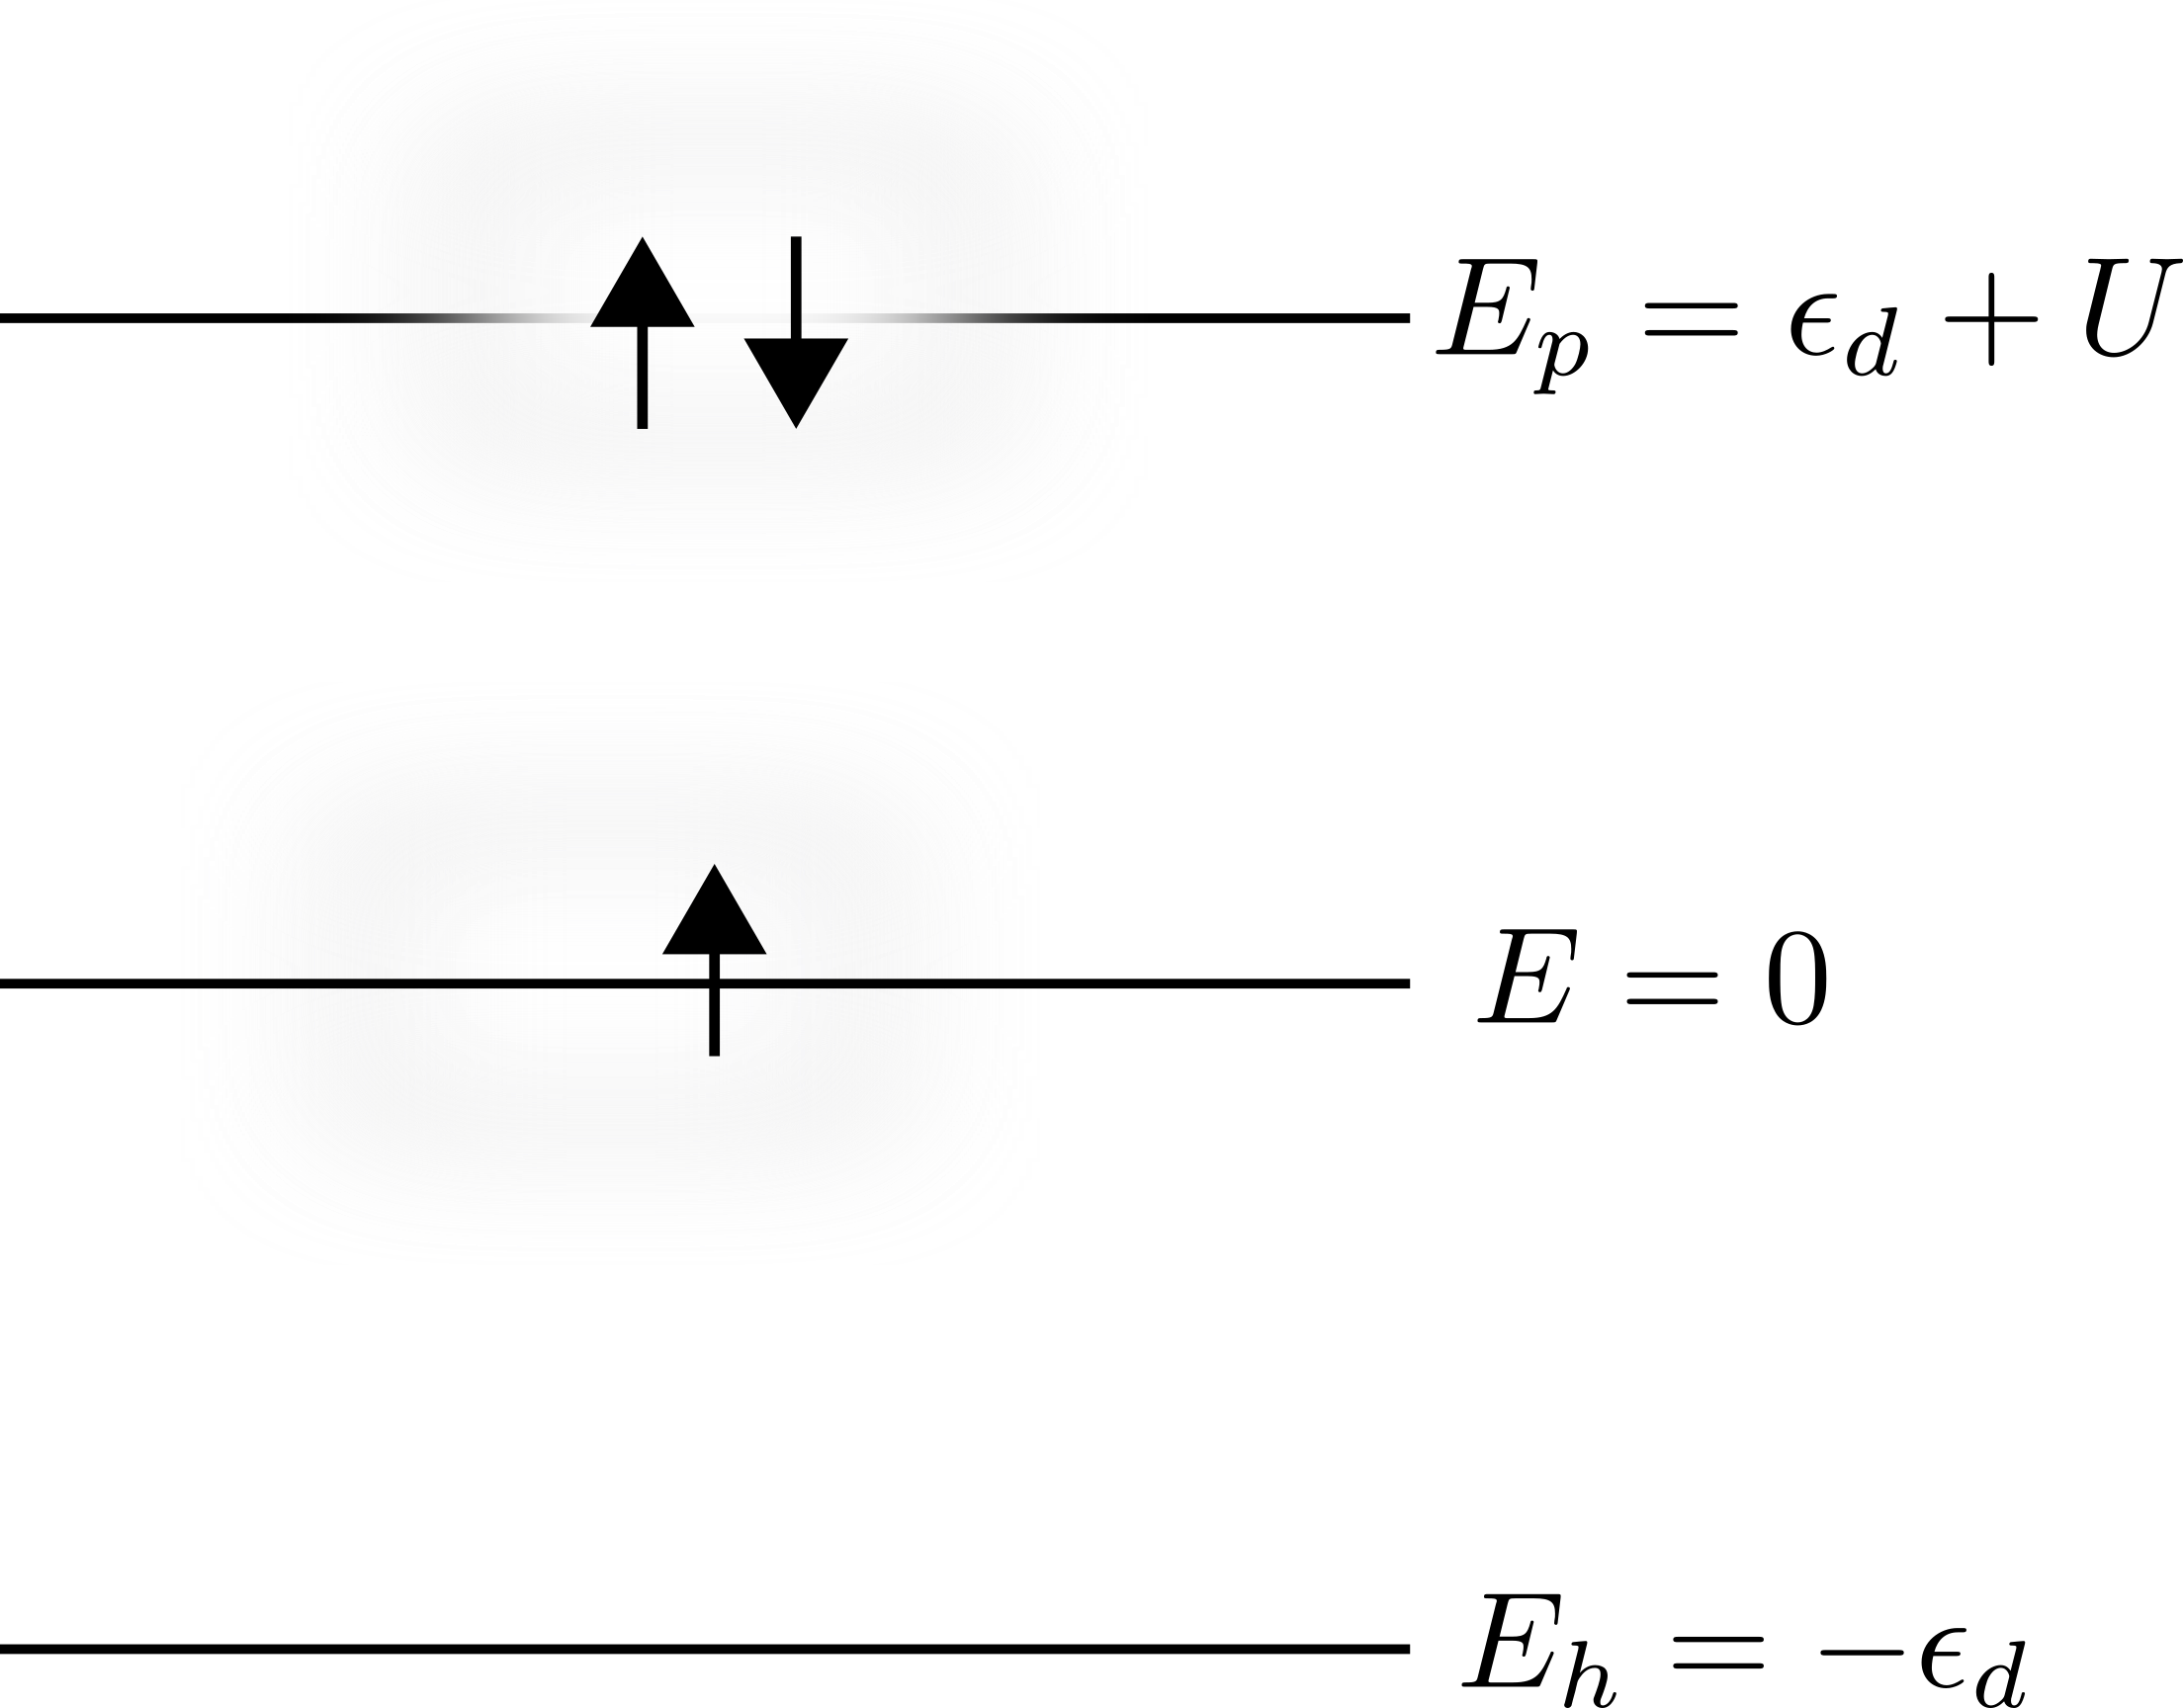
\includegraphics[scale=0.35]{phsymm.png}
	\captionof{figure}{Particle and hole excitations of the impurity}
\end{minipage}
\pb Since the URG is unitary, if we start from a model that is particle-hole symmetric, the RG equations should uphold that symmetry. What this means is that if we have \(\epsilon_d + \hf U = 0\) in the bare model, the new couplings should also satisfy \(\epsilon_d^\prime + \hf U^\prime = 0\). This means we must have 
\beq
\Delta\rr{\epsilon_d + \hf U} = 0
\eeq
The quantity \(\gamma = \epsilon_d + \hf U\) is thus an RG-invariant for the particle-hole symmetric model; it does not change under the RG flow. It is often referred to as the asymmetry parameter; it quantifies the asymmetry in the model. We need to check if our equations satisfy this. Looking at both the particle and hole equations, we can find the RG equation for the asymmetry parameter
\beq
\Delta^+\gamma\equiv\Delta^+\rr{\epsilon_d + \hf U} &= \sum_q |V(q)|^2\fr{1}{\omega^+ - \hf \epsilon_q - \epsilon_d + \hf J_z}\\
\Delta^-\gamma\equiv\Delta^-\rr{\epsilon_d + \hf U} &= -\sum_q |V(q)|^2\fr{1}{\omega^- - \hf\epsilon_q - \epsilon_d + \hf J_z}
\eeq
\comm{
At this point, we must note that \(\omega^+\) and \(\omega^-\), the quantum fluctuation energy scales, for the particle and hole sectors are not entirely independent. Recall that if we require the RG to be unitary, we must have \(\eta(\omega^-) = \rr{\eta^\dagger(\omega^+)}^\dagger\). This condition constrains the relation between \(\omega^\pm\). To see what the relation is, we can demand \(\Delta \gamma \equiv \Delta^+ \gamma + \Delta^- \gamma = 0\). That gives
\beq[phcond]
\omega^+  - \hf \epsilon_q = \omega^-  + \hf \epsilon_q
\eeq
}
For a particle-hole symmetric bare model, we can set \(\omega^+ = \omega^-\). That gives \(\Delta \gamma = 0\).

\subsection{"Poor Man's" one-loop form for asymmetric Anderson model}
In the limit of \(\epsilon_d, J \ll D \ll U \), the equation for \(\epsilon_d\) becomes, up to lowest order in \(J\),
\beq
\delta \epsilon_d = -\sum_q \fr{|V_q|^2 }{\omega^+ - \epsilon_q}
\eeq
If we assume an isotropic dispersion (\(\epsilon_q = D\)), where \(D\) is the current(running) bandwidth and a momentum-independent hopping potential \(V\),
\begin{gather*}
	\delta \epsilon_d = -\fr{1}{\omega^+ - D}\sum_q |V_q|^2 = -\fr{1}{\omega^+ - D}\rho(D) |\delta D| |V|^2
\end{gather*}
There we used 
\beq
\sum_q = \sum_{\epsilon_q\in\qq{D- |\delta D|, D}} = \rho(D) |\delta D|
\eeq
where \(\rho(D)\) is the single-spin density of states at the energy \(D\) and \(|\Delta D|\) is the thickness of the band that we disentangled at this step. In the literature, we usually define a quantity that denotes the amount of hybridisation between the impurity and the bath: \(\Delta \equiv \pi \rho(D) |V|^2\). In terms of this \(\Delta\), we get
\beq
\delta \epsilon_d = -\fr{\Delta |\delta D|}{\omega^+ - D}
\eeq
For low energy excitations, we can use \(\omega^+ \ll D\). Further, since we have defined \(\delta \epsilon_d = \epsilon_d(D-|\delta D|) - \epsilon_d(D)\), we must have \(\delta D = D - |\delta D| - D = - |\delta D|\).
\beq
\dv{\epsilon_d}{D} = -\fr{\Delta}{D}
\eeq
This is the form obtained from Poor Man's scaling of the asymmetric Anderson model.
\subsection{Vanishing of \(\Delta^6 \ham\)}\label{vanish}
If take the scattering term \(J_z \beta S^z_d c^\dagger_{q\beta}c_{k^\prime\beta}\) and construct the \(\eta\) and \(\eta^\dagger\) operators from them,
\beq
\eta &= \fr{1}{\omega^- - \hf\epsilon_q - \epsilon_d +  \beta J_z S^z_d}J_z \beta S^z_d c^\dagger_{k^\prime\beta}c_{q\beta}\\
\eta^\dagger &= \fr{1}{\omega^+ - \hf\epsilon_q - H_\text{imp} -  \beta J_z S^z_d}J_z \beta S^z_d c^\dagger_{q\beta}c_{k^\prime\beta}
\eeq
From the expression of \(\eta\), we can take its Hermitian conjugate to get another expression for \(\eta^\dagger\):
\beq
\eta^\dagger &= J_z \beta S^z_d c^\dagger_{q\beta}c_{k^\prime\beta}\fr{1}{\omega^- - \hf\epsilon_q - \epsilon_d +  \beta J_z S^z_d}\\
\eeq
Comparing the two expressions gives
\beq
\fr{1}{\omega^- - \hf\epsilon_q - \epsilon_d + \beta J_z S^z_d} = \fr{1}{\omega^+ - \hf\epsilon_q - H_\text{imp} - \beta J_z S^z_d}
\eeq
Substituting this equation into either \(\Delta^+_6\) or \(\Delta^-_6\) gives \(\Delta^+_6 \ham = -\Delta^-_6 \ham\), so \(\Delta_6 \ham = 0\).
\subsection{SU(2) invariance and Kondo model one-loop form}
Setting \(J_z = J_t = \hf J\) makes the interaction \(SU(2)\) symmetric; the last two RG equations can then be written in the common form:
\beq
2\Delta J_z = 2 \Delta J_t = \Delta J &= - J^2 \sum_{q}\fr{1}{\omega^+ - \hf\epsilon_q - \epsilon_d + \fr{1}{4}J}
\eeq
In order to reach the Kondo RG equations, we need to make the appropriate physical change; the difference between the Anderson model and the Kondo model is that the impurity charge fluctuations are frozen at single occupation in the latter. This means that the ground state of the impurity is now at \(\epsilon_d\). We can take account of this change by now measuring \(\omega^+\) from the single occupation energy itself, \(\epsilon_d\). Hence we should redefine \(\omega^+ - \epsilon_d \to \tilde \omega^+\). 
\beq[and2kondo]
2\Delta J_z = 2 \Delta J_t = \Delta J &= - J^2 \sum_{q}\fr{1}{\tilde \omega^+ - \hf\epsilon_q + \fr{1}{4}J}
\eeq
If we now consider low energy excitations (\(\tilde\omega^+ - \epsilon_q \approx  - \epsilon_q\)) and expand the denominator in powers of \(J\) and keep only the lowest order, we get
\beq
\Delta J = -J^2 \sum_q \fr{1}{-\hf\epsilon_q}
\eeq
For an isotropic dispersion, we can use \(\epsilon_q = D\). The sum can then be evaluated as
\beq
\sum_q = \rho(D)\Delta D
\eeq
The flow equation of \(J\) becomes
\beq
\Delta J = 2J^2 \rho(D)\fr{|\Delta D|}{D}
\eeq
This is the familiar one-loop Kondo flow equation obtained from Poor man's scaling. To get the continuum version, we must note that since we are decreasing the bandwidth, we have to set \(\Delta D = -|\Delta D|\). Therefore,
\beq
\dv{J}{\ln D} = -2J^2 \rho(D)
\eeq
\subsection{Connection with Kondo URG result}
Recall eq.~\ref{and2kondo}.
\beq
\Delta J = - J^2 \sum_{q}\fr{1}{\tilde \omega^+ - \hf\epsilon_q + \fr{1}{4}J}
\eeq
For \(\tilde \omega^+ = 0\) and \(\epsilon_q = D\), we get
\beq
\Delta J = 2J^2 \sum_{q}\fr{1}{D - \fr{1}{2} J}
\eeq
This has the same fixed point structure as the Kondo URG scaling equation.
\comm{
\subsection{Fixed points for the symmetric Anderson model with \(J_z = J_t\)}
We first consider the simpler case where \(\epsilon_d + \hf U = 0\), \(J_z = J_t = \hf J\) and \(\omega^+ = \omega^-\). We also assume an isotropic dispersion \(\epsilon_q =D\) and momentum independent potential \(V(q)\equiv V\). For convenience, we define \(n(D) = \sum_{\epsilon_q=D}\) and \(\mc{V}(D) = \sum_{\epsilon_k<D}\). The former is the number of states on the energy shell at \(D\), while the latter is the number of states inside the energy shell \(D\). The combined (particle+hole) scaling equations become:
\begin{flalign*}
	\Delta U &= -\fr{|V|^2 n(D)\rr{2U +  J}}{\rr{\omega - \hf D + \hf U + \fr{1}{4} J}\rr{\omega - \hf D}} - \fr{\fr{1}{8}J^2n(D) \mc{V}(D)\qq{6\rr{\omega - \hf D + \hf U} - J}}{\rr{\omega - \hf D + \hf U + \fr{1}{4}J}\rr{\omega - \hf D + \hf U - \fr{1}{4}J}}\\
\Delta V &= -\fr{5}{8}J V n(D)\fr{1}{\omega - \hf D + \hf U + \fr{1}{4} J}\\
\Delta J &= -J^2 n(D) \fr{1}{\omega - \hf D + \hf U + \fr{1}{4} J}\\
\end{flalign*}
\subsubsection*{In absence of Kondo-type interaction (\(\pmb{J=0}\))}
We first consider the case where \(J=0\). The only relevant equation is then that of \(U\), because \(V\) and \(J\) will then not flow.
\beq
\Delta U &= \fr{-2|V|^2 U n(D)}{\rr{\omega - \hf D}\rr{\omega - \hf D + \hf U}}
\eeq
To get a feel for this equation, we look at a specific value of \(\omega = \hf U\). For this value,
\beq
\Delta U &= \fr{|V|^2 U n(D)}{D\rr{D - \hf U}}
\eeq
If we start with bare values \(U\) and \(D\) such that \(U <  2D\), then \(U\) is relevant, and it will increase. Meanwhile, the bandwidth will decrease as we go to lower energies. The fixed point is achieved when the denominator becomes zero.
\beq
U^* = 2 D^*
\eeq
The opposite thing happens if we start with bare values such that  \(U >  2D\). Then, \(U\) is irrelevant and it will decrease until it reaches the same fixed point condition. This fixed point, characterized by \(U^* = 2 D^*\) and \(J=0\), is the \textit{local moment fixed point}. It is stable along both directions in the \(U-\)axis. It is however unstable to perturbations in \(J\), as we will see later.
\pb
There is another fixed point in this picture, the free orbital fixed point at \(U=V=0\). It is unstable in all directions. The two fixed points and the flows are schematically shown in fig.~\ref{lmflow}. One specific flow line for \(J=0\) is shown in fig.~\ref{fo2lm}.
\begin{figure}
\centering
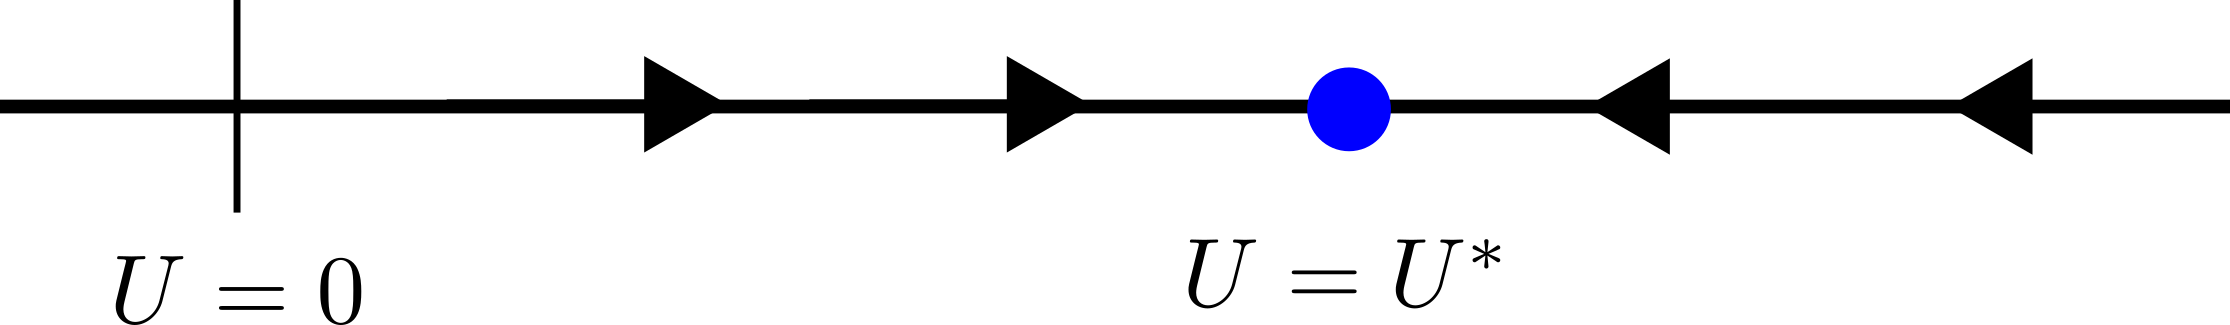
\includegraphics[scale=0.5]{lmflow.png}
\caption{Flows towards local moment for \(J=0\)}
\label{lmflow}
\end{figure}
\begin{figure}
\centering
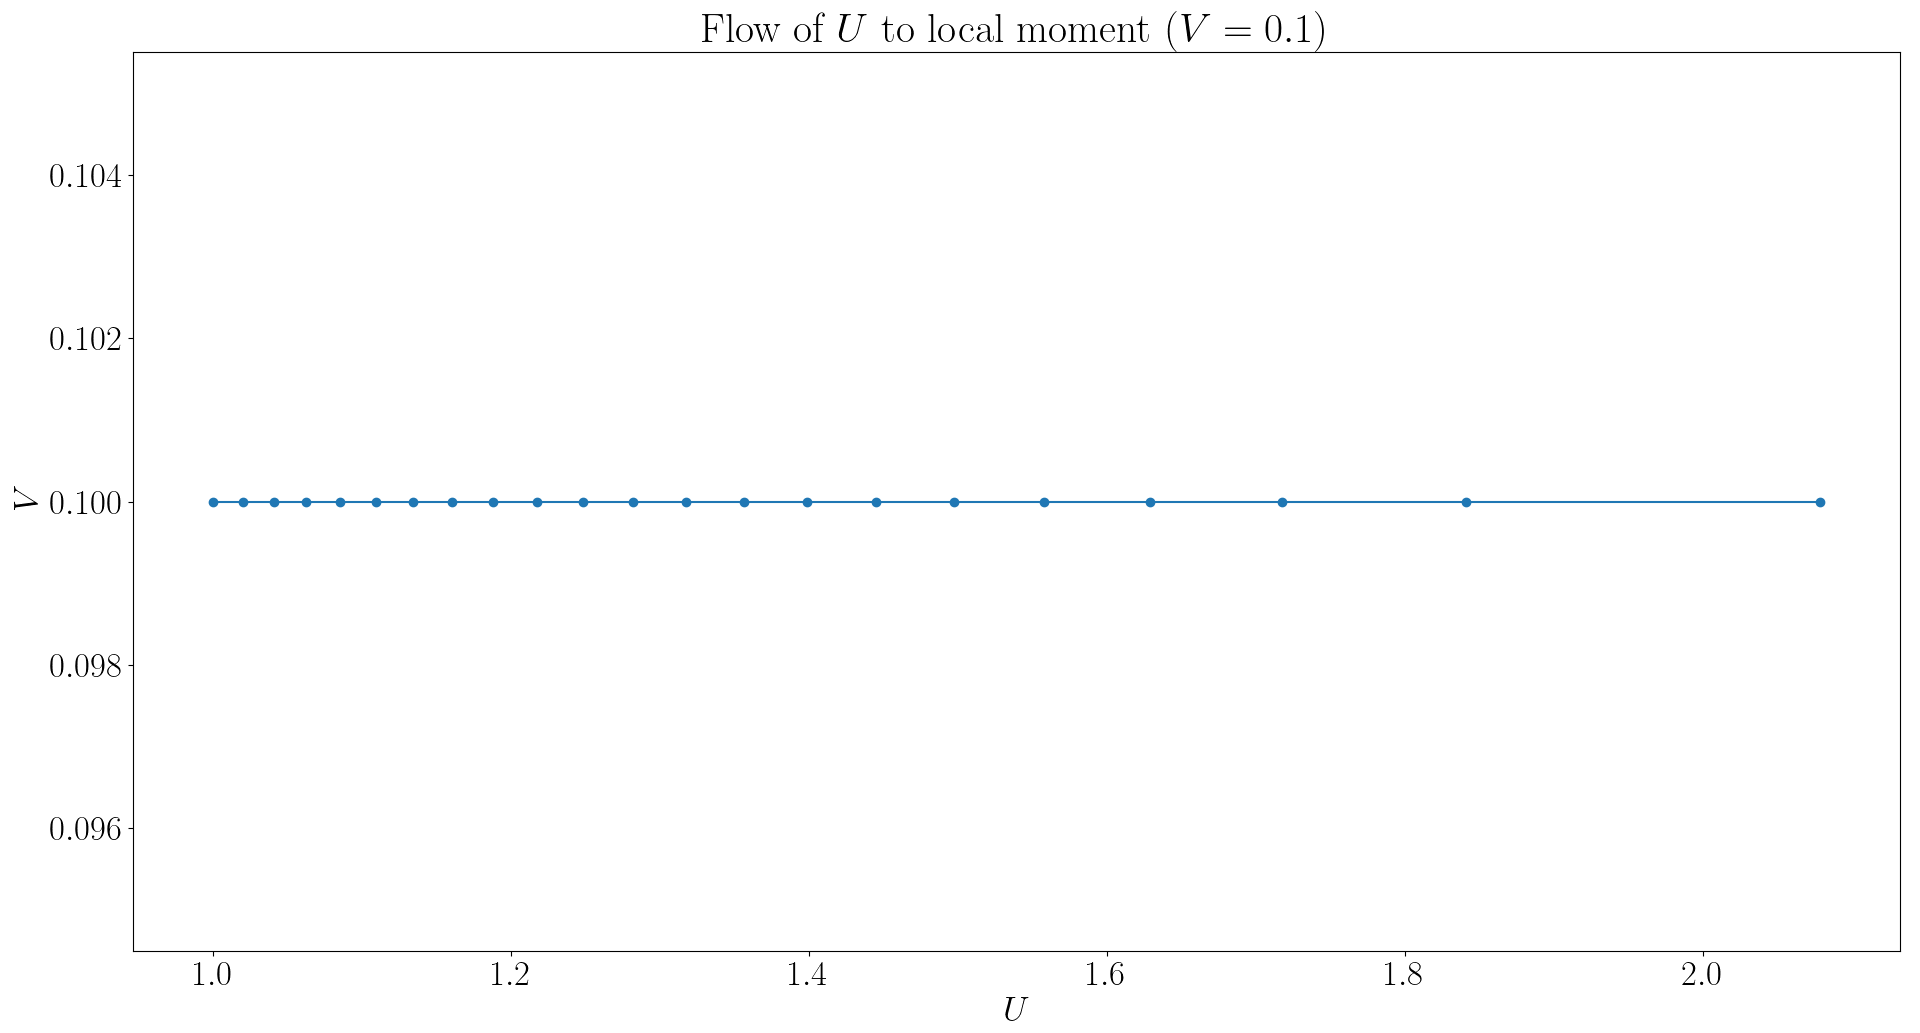
\includegraphics[scale=0.3]{fo2lm.png}
\caption{Plot of a particular flow from free orbital (leftmost) to local moment (rightmost) for \(J=0\)}
\label{fo2lm}
\end{figure}
\subsubsection*{With the Kondo-type interaction (\(\pmb{J>0})\)}
In this case, all three equations will come into play. Using the value \(\omega^- = \hf U + \hf J\), the equations become
\begin{flalign*}
\Delta U &= \fr{|V|^2\rr{U + \hf J}n(D)}{\rr{D - \fr{1}{4}J}\rr{D - \hf U - \hf J}} + \fr{1}{8} \fr{J^2n(D)\mc{V}(D)\qq{6D - 2J}}{\rr{D - \fr{1}{4}J}\rr{D - \fr{3}{4}J}}\\
\Delta V &= \fr{3}{4}Jn(D)V\fr{1}{D - \fr{1}{4}J}\\
\Delta J &= \hf J^2 n(D)\fr{1}{D - \fr{1}{4}J}
\end{flalign*}
We can now see how the couplings will flow if we start at the local moment fixed point and add a small perturbation \(J\). Because of the condition for the local moment fixed point, we know that \(D^* - \hf U^* = 0\). Also, close to the local moment, \(J\) is small so we can ignore the \(J^2\) term. The equations thus become
\begin{flalign*}
\Delta U &= -2\fr{|V|^2\rr{U^* + \hf J}n(D)}{\rr{D^* - \fr{1}{4}J}J} < 0\\
\Delta V &= \fr{3}{4}Jn(D)V\fr{1}{D^* - \fr{1}{4}J} > 0\\
\Delta J &= \hf J^2 n(D)\fr{1}{D^* - \fr{1}{4}J}>0
\end{flalign*}
The \(U\) is irrelevant and will flow down. The \(J\) on the other hand is relevant and will flow to some large value. This fixed point, characterized by a large positive \(J\) is the strong-coupling fixed point.
\pb
\begin{minipage}{250pt}
	A similar flow happens if we start from the free orbital fixed point. There, \(U\) is 0, and the equations look like
\begin{flalign*}
\Delta U &= \hf \fr{|V|^2Jn(D)}{\rr{D - \fr{1}{4}J}\rr{D - \hf J}} > 0\\
\Delta V &= \fr{3}{4}Jn(D)V\fr{1}{D - \fr{1}{4}J} > 0\\
\Delta J &= \hf J^2 n(D)\fr{1}{D - \fr{1}{4}J}>0
\end{flalign*}
Here both \(U\) and \(J\) are relevant and they flow up to the strong-coupling fixed point. A schematic flow diagram is shown in fig.~\ref{schemesc}.
\end{minipage}
\hspace*{30pt}\begin{minipage}{250pt}
\centering
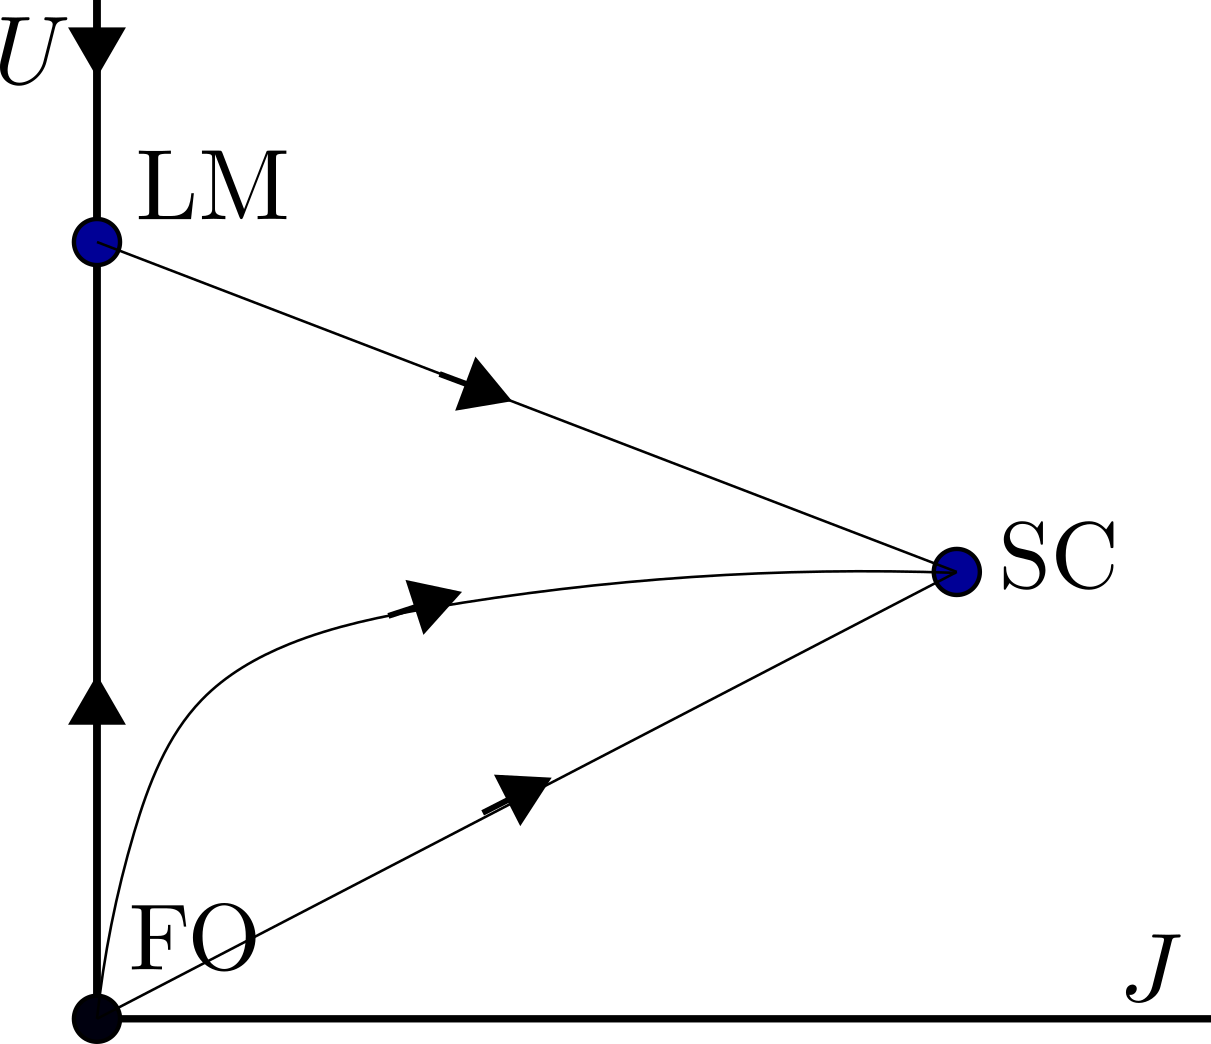
\includegraphics[scale=0.65]{schematic.png}
\captionof{figure}{Schematic flows from local moment and free orbital to strong-coupling}
\label{schemesc}
\end{minipage}
}
\section{Connection between Unitary Renormalization Group and Poor Man's Scaling}
We first motivate the formalism of PMS method. The problem is defined as
\beq[problem]
\ham\ket{\Psi} = E\ket{\Psi}
\eeq
\(\ham\) is the total Hamiltonian and \(\ket{\Psi}\) and \(E\) are the exact eigenstate and eigenvalue of \(\ham\). The problems we deal with typically have a bath of mobile electrons, with energies spanning from \(-D\) to \(D\). We are interested in finding effective Hamiltonians after "removing" the highest shell in the conduction bath. This will give us a Hamiltonian to which we can again apply the same procedure.
\pb We want to decouple one electron at momentum \(q\). We can split the exact wavefunction as
\beq[wf]
\ket{\Psi} = \ket{\Psi_0} + \ket{\Psi_1}
\eeq
where \(\ket{\Psi_0} = \rr{1 - \hat n_{q}}\ket{\Psi^N}\) is that part of the wavefunction where the state \(q\) is occupied. \(\ket{\Psi^N_1} = \hat n_q \ket{\Psi}\) is that part of the wavefunction where the state \(q\) is occupied. We can also split the Hamiltonian as
\beq[hami]
\ham = \ham^d + V_0 + V_+ + V_-
\eeq
\(\ham^d\) is the diagonal part; it has the purely energy terms as well as self-energies that may arise from the diagonal parts of interactions; \(V_0\) is the purely off-diagonal term that does not change \(\hat n_q\); it is the scattering \textit{inside} the low energy subspace. \(V_+\) and \(V_-\) are the purely off-diagonal terms that \textit{do} change \(\hat n_q\); \(V_+\) takes you from \(\hat n_q = 0\) to \(\hat n_q = 1\) and \(V_-\) does the opposite.
\pb Substituting eqs.~\ref{hami} and \ref{wf} in eq.~\ref{problem} gives
\beq
\rr{\ham^d + V_0 + V_+ + V_-}\rr{\ket{\Psi_0} + \ket{\Psi_1}} = E\rr{\ket{\Psi_0} + \ket{\Psi_1}}
\eeq
Gathering the kets with \(\hat n_q = 0,1\) gives
\beq
\rr{\ham^d_0 + V_0}\ket{\Psi_0} + V_- \ket{\Psi_1} = E\ket{\Psi_0}\\
\rr{\ham^d_1 + V_0}\ket{\Psi_1} + V_+\ket{\Psi_0} = E\ket{\Psi_1}
\eeq
The second equation can be written as
\beq
\ket{\Psi_1} = \eta^\dagger \ket{\Psi_0}
\eeq
where
\beq
\rr{\eta^\dagger}_\text{PMS} = \fr{1}{E - \ham^d_1 - V_0}V_+
\eeq
Substituting this in the second equation gives
\beq[reneq]
\rr{\ham^d_0 + V_0 + V_- \eta^\dagger}\ket{\Psi_0} = E\ket{\Psi_0}
\eeq
This new Hamiltonian,
\beq
\tilde \ham_0 = \ham^d_0 + V_0 + V_- \eta^\dagger
\eeq
has the high energy mode removed; the scattering terms start from the low energy subspace and end at the low energy subspace as well. The renormalization in the low energy subspace scatterings  is
\beq[deltaV]
\Delta V_0 = V_- \eta^\dagger
\eeq
If we eliminate \(\ket{\Psi_0}\) instead of \(\ket{\Psi_1}\), we get the renormalized equation in the high energy subspace:
\beq
\ket{\Psi_0} = \eta \ket{\Psi_1}
\eeq
where
\beq
\rr{\eta}_\text{PMS} = \fr{1}{E - \ham^d_0 - V_0}V_-
\eeq
,so
\beq
\rr{\ham^d_1 + V_0 + V_+ \eta}\ket{\Psi_1} = E\ket{\Psi_1}
\eeq
The renormalized Hamiltonian in the high energy subspace is thus
\beq
\tilde \ham_1 = \ham^d_1 + V_0 + V_+ \eta
\eeq
If we want to keep both the high energy and low energy parts of the Hamiltonian, the new Hamiltonian is
\beq[transham]
\tilde \ham &= \tilde \ham_1 \hat n + \tilde \ham_0 \rr{1 - \hat n}\\
&= \ham^d_0 + \ham^d_1 + V_0 + V_+ \eta + V_- \eta^\dagger
\eeq
The total renormalization is
\beq
\rr{\Delta \ham}_\text{PMS} = V_+ \rr{\eta}_\text{PMS} + V_- \rr{\eta^\dagger}_\text{PMS}
\eeq
It can be shown that if we define a unitary operator \(U = 1 - \eta + \eta^\dagger\), the transformed Hamiltonian \(U \ham U^\dagger\) is the same as eq.~\ref{transham}. This, along with the properties of \(\eta\), have been shown in section \ref{urgform}. The important feature of eq.~\ref{transham} is that there is no term in the transformed Hamiltonian which scatters between \(\ket{\Psi_0}\) and \(\ket{\Psi_0}\)- the two subspaces have been truly decoupled.
\beq
\qq{U \ham U^\dagger, n_q} = 0
\eeq
We can write down the renormalized Schrodinger equation in the low energy subspace, from eq.~\ref{reneq},
\beq
\tilde \ham_0 \ket{\Psi_0} = E\ket{\Psi_0}
\eeq
and again repeat the entire process. \(\tilde \ham_0\) now takes the place of \(\ham\) and \(\ket{\Psi_0}\) takes the place of \(\ket{\Psi}\) in eq.~\ref{problem}.
\pb The expression for URG is obtained in an almost identical way. The only difference is that instead of starting with the exact eigenpair (\(E,\ket{\Psi}\)), we start with a more general pair (\(\tilde \ham, \ket{\Phi}\)) where \(\ket{\Phi}\) is not necessarily an exact eigenstate of \(\ham\). It is defined by \(\ham^\prime\), which is in turn defined as \(\hat n_q \ham^\prime\rr{1 - \hat n_q} = 0\). \(\ket{\Phi}\) is then defined by
\beq
\ham\ket{\Phi} = \ham^\prime \ket{\Phi}
\eeq
This definition of \(\ham^\prime\) is the very minimum that we must have in order to fulfill our goal (decouple \(q\)). 
\pb The operators \(\eta\) and its conjugate change accordingly:
\beq
\rr{\eta}_\text{URG} &= \fr{1}{\tilde\ham - \ham^d_0 - V_0}V_-\\
     &= \fr{1}{\hat \omega - \ham^d_0}V_-\\
\eeq
where \(\hat \omega \equiv \ham^\prime - V_0\) now embodies the quantum fluctuations inherent in the Hamiltonian through the scattering term \(V_0\). Similarly,
\beq
\rr{\eta^\dagger}_\text{URG} &= \fr{1}{\hat \omega - \ham^d_1}V_+\\
\eeq
The renormalization is again
\beq
\rr{\Delta \ham}_\text{URG} = V_+\rr{\eta}_\text{URG} + V_-\rr{\eta^\dagger}_\text{URG}
\eeq
This again allows us to write down a unitary operator that decouples the entangled state:
\beq
U =  1 - \eta + \eta^\dagger, \qq{\hat n_q, U \ham U^\dagger} = 0
\eeq
where \(\tilde \ham = U^\dagger \ham U\). We can now write down a new problem in this decoupled space with the rotated items and attempt to decouple another electron \(q^\prime\). We will again choose some general eigenpair (\(\ham^\prime,\ket{\Phi}\)) such that \(\tilde\ham\ket{\Phi} = \ham^{\prime}\ket{\Phi}\) and \(\qq{\ham^{\prime},\hat n_{q^\prime}}=0\).
\pb Summarizing, the general Hamiltonian is not diagonal in the Fock space basis.
URG, in order to proceed, selects one non-Fock basis of states \(\ket{\Phi}\) such that \(q\) is decoupled in that Hamiltonian.
Since there can be lots of such basis, there is a freedom in this choice.
With this basis in mind, URG then finds a unitary operator which when operated on the Hamiltonian takes me to the form in which it is diagonal in the Fock space basis.
Note that this form is a function of the chosen \(\ket{\Phi}\).
We then select the second degree of freedom and repeat the process.
What PMS does is, it exploits the freedom of choice and selects the exact eigenstate \(\ket{\Psi}\) of the Hamiltonian as the non-Fock basis \(\ket{\Phi}\).
Doing that returns a rotated Hamiltonian which is diagonal in \(q\), and is a function of the chosen state, same as URG. The conclusion is that depending on which state we choose as our diagonal non-Fock basis, URG and PMS will cause flows along different lines in general.
\pb As the couplings flow, \(V_0\) will also flow, leading to a flow of \(\hat\omega\). Just at the fixed point, the denominator of URG vanishes, giving the equation
\beq
\rr{\hat\omega - \ham_1^d}V_+\ket{\Psi_0} \text{ or } \rr{\hat\omega - \ham_1^d}V_-\ket{\Psi_1}
\eeq
This means that one of the eigenvalues of \(\hat\omega\) matches with the eigenvalue of the diagonal part \(\ham^d\), either in the occupied sector (\(\ham^d_1\)) or unoccupied sector (\(\ham^d_1\)). Since the eigenvalues are unchanged during the unitary renormalization, this implies that \(\omega\) takes up one of the eigenvalues of the whole Hamiltonian \(\ham\). This will correspond to the fixed point obtained from PMS if we had started PMS with that eigenvalue.
\pb In short, while the PMS flow is parametrised by one of the exact energy eigenvalues \(E\), the URG flow is parametrised by a non-trivial operator \(\hat \omega\) which incorporates both a diagonal part and an off-diagonal part and itself flows under the URG. At the fixed point, the off-diagonal part cancels out and the \(\hat\omega\) finally flows to one of the energy eigenvalues and the URG fixed point matches with one of the PMS fixed points.
\begin{center}
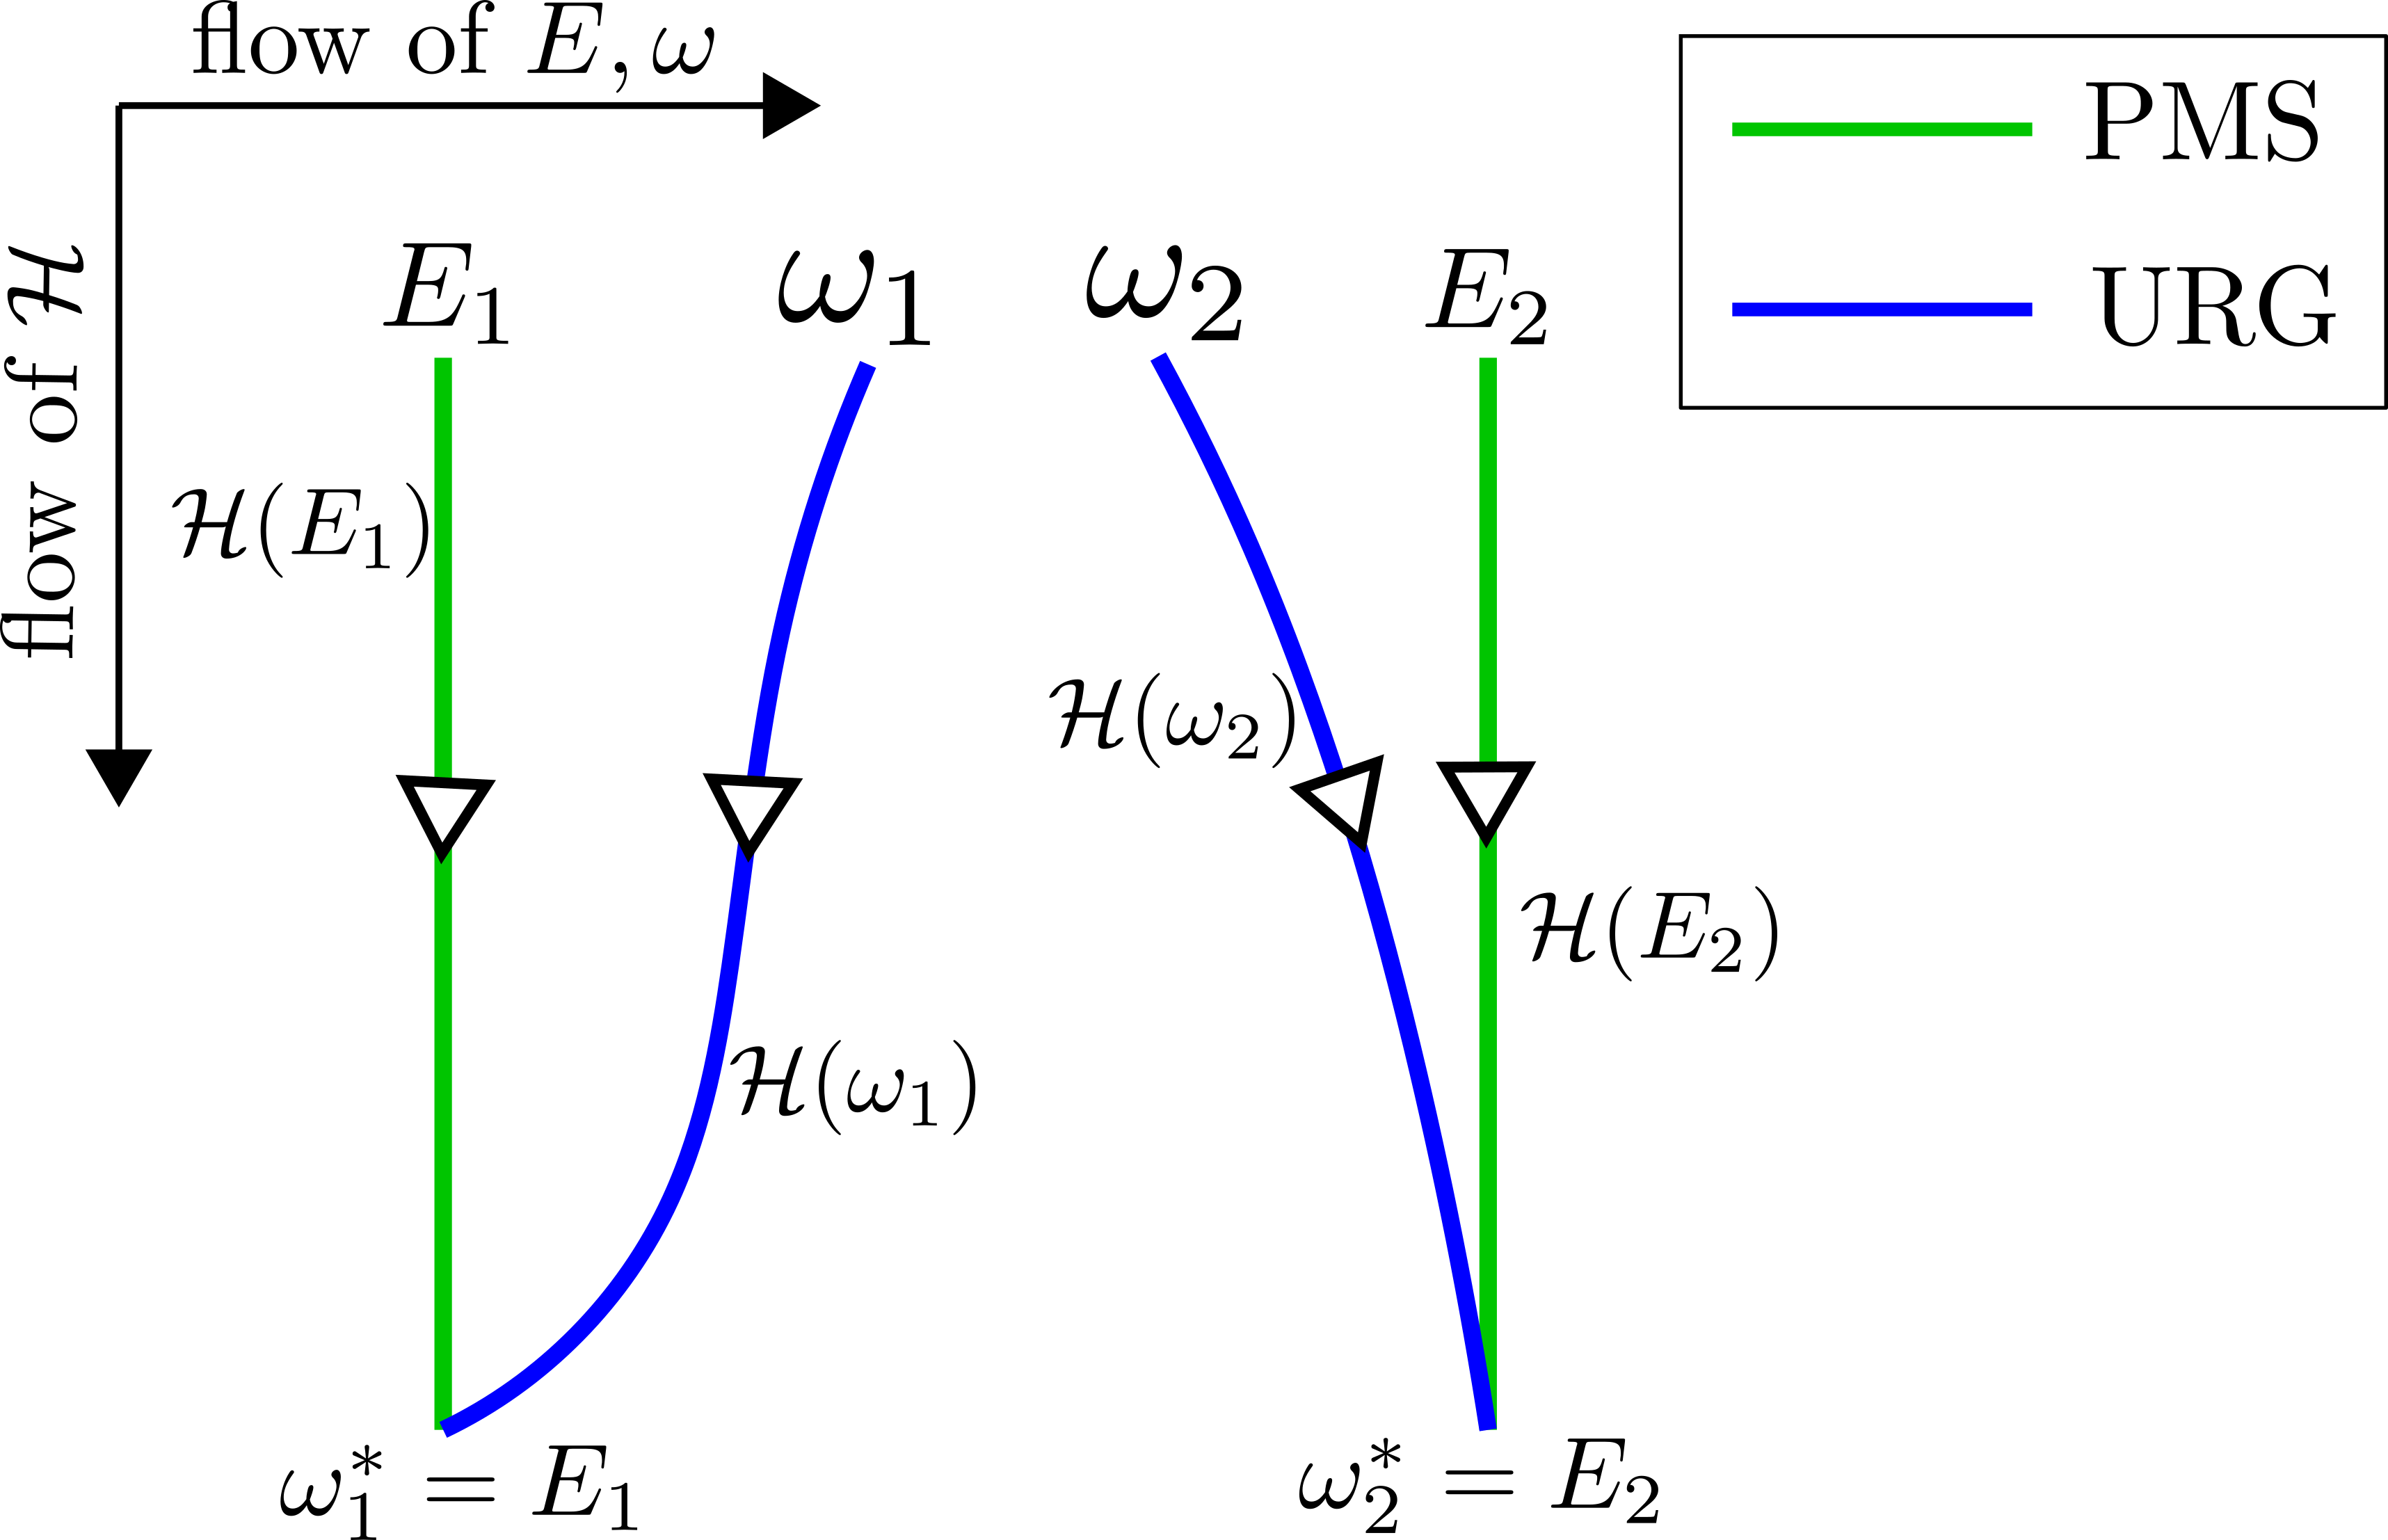
\includegraphics[scale=0.42]{pms_vs_urg.png}
\captionof{figure}{Flows of PMS(green) and URG(blue)}
\end{center}
To demonstrate the implementation, we can look at a specific model. For the SIAM,
\beq
\ham = \sum_{k\sigma}\rr{\epsilon_k \tau_{k\sigma} + V c^\dagger_{k\sigma}c_{d\sigma} + \text{h.c.}}
\eeq
We want to decouple the state \(q\beta\) from the rest of the electrons. We have \(\hat\ham_0 = \epsilon_d\hat n_d + U \hat n_{d\ua}n_{d\da} + \sum_{k\sigma} \epsilon_k \hat n_{k\sigma}\), \(V_0 = \sum_{k<q,\sigma}c^\dagger_{k\sigma}c_{d\sigma}+\text{h.c.}\), \(V_+ = V c^\dagger_{q\beta}c_{d\beta}\) and \(V_- = V c^\dagger_{d\beta}c_{q\beta}\). The renormalization in particle sector
\beq
\Delta V_0 &=  c^\dagger_{d\beta}c_{q\beta}\fr{1}{\rr{E - V_0} - \hat \ham^d_0}c^\dagger_{q\beta}c_{d\beta}\\
\eeq
The intermediate energy (at the propagator) is
\beq
\hat \ham^d_0 = \sum_{k,\sigma}\epsilon_k \tau_{k\sigma} + \epsilon_d \hat n_{d\ol\beta}
\eeq
This is because the \(c_{d\beta}\) at the right of the propagator ensures that we must have \(\hat n_{d\beta}=0\) at the propagator.
\beq
\Delta V_0 &=  c^\dagger_{d\beta}c_{q\beta}\fr{1}{\rr{E - V_0} - \sum_{k,\sigma}\epsilon_k \tau_{k\sigma} - \epsilon_d \hat n_{d\ol\beta}}c^\dagger_{q\beta}c_{d\beta}\\
\eeq
Since \(E\) is the exact eigenvalue, we do not have an expression for it. Instead, we approximate \(E - V_0\) by substituting it with the current diagonal part corresponding to the initial state on which this entire term will act. The intial state is characterized by \(\hat n_{q\beta}=0\) and \(\hat n_{d\beta} = 1\), so
\beq
E - V_0= \sum_{k<q,\sigma}\epsilon_k \tau_{k\sigma} - \hf\epsilon_q + \epsilon_d + \rr{\epsilon_d + U}\hat n_{d\ol\beta}
\eeq
The \(- \hf\epsilon_q\) comes from substituting \(\hat n_{q\beta}=0\) in \(\epsilon_q \tau_{q\beta}\).
\pb  Substituting this in \(\Delta V_0\) gives
\beq
\Delta V_0 &=  c^\dagger_{d\beta}c_{q\beta}\fr{1}{-\hf\epsilon_q -\epsilon_q \tau_{q\beta} + \epsilon_d + U\hat n_{d\ol\beta}}c^\dagger_{q\beta}c_{d\beta}\\
&=  c^\dagger_{d\beta}c_{q\beta}\fr{1}{-\epsilon_q + \epsilon_d + U\hat n_{d\ol\beta}}c^\dagger_{q\beta}c_{d\beta}\\
&=  c^\dagger_{d\beta}c_{q\beta}c^\dagger_{q\beta}c_{d\beta}\fr{1}{-\epsilon_q + \epsilon_d + U\hat n_{d\ol\beta}}\\
&=  -c^\dagger_{d\beta}c_{q\beta}c^\dagger_{q\beta}c_{d\beta}\fr{1}{\epsilon_q - \epsilon_d - U\hat n_{d\ol\beta}}\\
&=  \rr{1 - \hat n_{q\beta}}\rr{\fr{-\hat n_{d\beta}\hat n_{d\ol\beta}}{\epsilon_q - \epsilon_d - U} + \fr{-\hat n_{d\beta}\rr{1 - \hat n_{d\ol\beta}}}{\epsilon_q - \epsilon_d}}\\
\eeq
On the second line, we substituted \(\tau_{q\beta} = \hf\) in the denominator, which is ensured by the \(c^\dagger_{q\beta}\) to the right of the propagator. The first term renormalizes the energy of the doublon state and the second term renormalizes that of the singly-occupied state:
\beq
\Delta E_2 &= \fr{-1}{\epsilon_q - \epsilon_d - U}\\
\Delta E_1 &= \fr{-1}{\epsilon_q - \epsilon_d}
\eeq
The renormalization in the hole sector is
\beq
\Delta V_0 &=  c^\dagger_{q\beta}c_{d\beta}\fr{1}{\rr{E - V_0} - \hat \ham^d_0}c^\dagger_{d\beta}c_{q\beta}\\
	   &=  c^\dagger_{q\beta}c_{d\beta}\fr{1}{\rr{E - V_0} - \sum_{k,\sigma}\epsilon_k\tau_{k\sigma} - \epsilon_d - \rr{\epsilon_d + U}\hat n_{d\ol\beta}}c^\dagger_{d\beta}c_{q\beta}
\eeq
This time we substitute
\beq
E - V_0 &= \sum_{k<q,\sigma}\epsilon_k \tau_{k\sigma} + \tau_{q\beta} \epsilon^-_q + \epsilon_d\hat n_{d\ol\beta}\\
&= \sum_{k<q,\sigma}\epsilon_k \tau_{k\sigma} + \hf \epsilon^-_q + \epsilon_d\hat n_{d\ol\beta}\\
\eeq
In the last step we put \(\tau_{q\beta}=\hf\) because the state is occupied in the initial configuratin. Note that since the electron \(q\beta\) was occupied in the intial state, the energy \(\epsilon^-_q\) in this sector must be opposite to that of the particle sector, \(\epsilon_q\). Hence \(\epsilon^-_q = -\epsilon_q\), which gives
\beq
\Delta V_0 & = c^\dagger_{q\beta}c_{d\beta}\fr{1}{-\hf \epsilon_q -\epsilon^-_q\tau_{q\beta} - \epsilon_d - U\hat n_{d\ol\beta}}c^\dagger_{d\beta}c_{q\beta}\\
& = c^\dagger_{q\beta}c_{d\beta}c^\dagger_{d\beta}c_{q\beta}\fr{1}{-\epsilon_q - \epsilon_d - U\hat n_{d\ol\beta}}\\
& = \hat n_{q\beta}\rr{\fr{-\rr{1 - \hat n_{d\beta}}\hat n_{d\ol\beta}}{\epsilon_q + \epsilon_d + U} + \fr{-\rr{1 - \hat n_{d\beta}}\rr{1 - \hat n_{d\ol\beta}}}{\epsilon_q + \epsilon_d}}\\
\eeq
In the second line, we put \(\epsilon^-_q = -\epsilon_q\) and \(\tau_{q\beta} = -\hf\). The first term renormalizes the singly-occupied state while the second term renormalizes the holon state. Combining with the particle sector results, the total renormalization in all the three impurity states (holon, single and doublon) are
\beq
\Delta E_0 &= -\fr{1}{\epsilon_q + \epsilon_d}\\
\Delta E_1 &= -\fr{1}{\epsilon_q + \epsilon_d + U} - \fr{1}{\epsilon_q - \epsilon_d}\\
\Delta E_2 &= -\fr{1}{\epsilon_q - \epsilon_d - U}\\
\eeq
These results are also obtained in ref.~\cite{hewson}. The complete process is depicted in fig.~\ref{pmsflow}.
\pb \textbf{Some conclusions}:
\begin{itemize}
	\item The \it{only} difference in the formalism of PMS and URG is that while PMS uses the exact energy eigenvalue \(E\) to parameterise the flow, URG uses a general intermediate decoupled Hamiltonian to do the same. Since the \(E\) is also, technically, an intermediate decoupled Hamiltonian (it is the final Hamiltonian), PMS can be seen as an URG but with a specific choice for the paramter.
	\item In practise, PMS replaces \(E-V_0\) with the diagonal part of the initial state at the current step of the RG. There are several points to make here. We are talking about the energy of the initial state, not the intermediate state. This is because, from eq.~\ref{problem}, \(E\) is the energy of the initial state on which \(V_\pm\) act. 
	\item The ideal solution would have been to substitute the exact energy and the total scattering term \(V\), but since we do not know \(E\) and keeping the \(V\) would make the thing untractable, we use our current best guess (renormalised diagonal part). As the RG flows, both \(E_j\) and \(V\) flow, such that at the fixed point, \(V\) becomes zero (scattering terms get removed) and \(E_j\) morphs into the exact \(E\). 
	\item In practise, URG replaces the \(\hat \omega\) with a guess for the final energy \(E\). This however ignores the renormalization of \(\hat \omega\). A better approach would be to replace it with \(E_j\), following PMS. That would act like the one-particle renormalization of \(\hat \omega\).
	\item PMS mostly drops any diagonal component of the scattering from the denominator. For example, in the PMS of the Kondo model by Anderson \cite{Anderson} or that of the anisotropic power law Kondo model by Chenge et.al \cite{tatha}, they do not keep the term \(J_z S_d^z s^z\) in the denominator although it is number(spin) conserving. Such terms are kept in the denominator of the URG though. It must be mentioned however that ref.~\cite{raja} does bring a diagonal charge-charge interaction in the denominator in the PMS of the extended Anderson model.
\end{itemize}
\begin{figure}
	\centering
	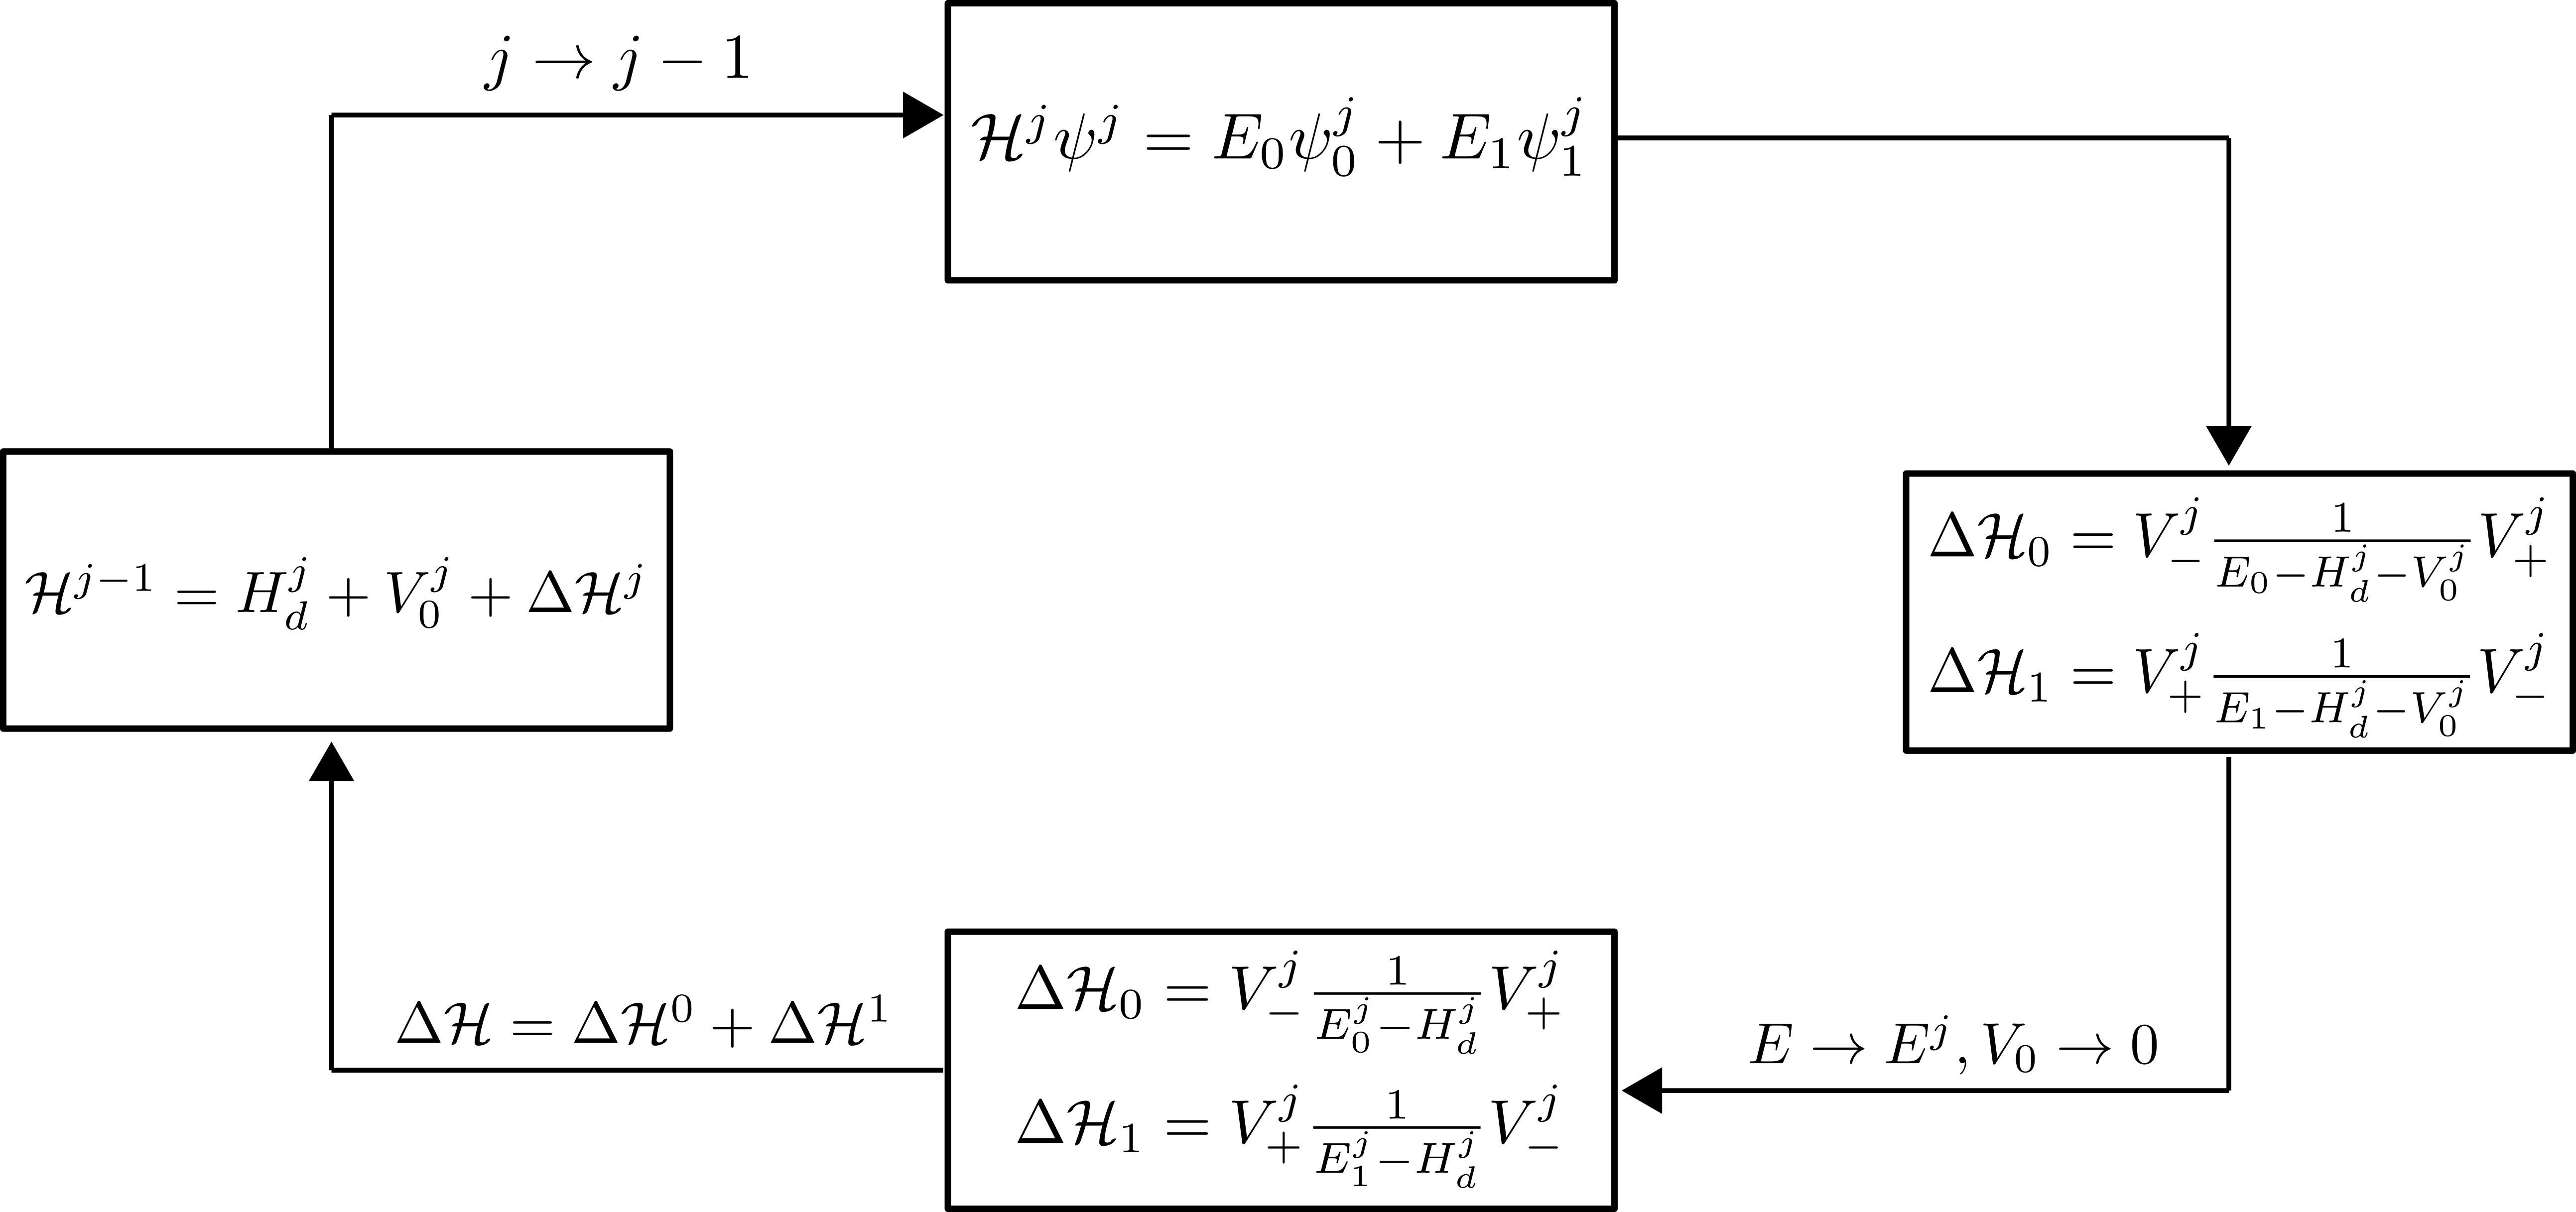
\includegraphics[scale=0.35]{pms-flowchart.png}
	\caption{Flow chart of "Poor Man's" scaling algorithm}
	\label{pmsflow}
\end{figure}
\comm{
	\There are two terms. The two terms differ in their initial states; one starts from \(n_{d\ol\beta}=1\) (corresponding to \(E^a\)) and the other starts from \(n_{d\ol\beta}=0\) (corresponding to \(E^b\)). From the definition of the \(T-\)matrix we can see that different initial states will give rise to different final eigenstates. To treat the various energies \(E^a\) and \(E^b\) on an equal footing, we need to subtract off the initial energies:
\beq
E_0 &= \epsilon_d + \rr{\epsilon_d + U}\hat n_{d\ol\beta}\\
\implies E^a_0 &= 2\epsilon_d + U\\
E^b_0 &= \epsilon_d
\eeq
Defining \(\xi = E - E_0\),
We can then write
\beq
\Delta V_P &= \rr{\fr{\hat n_{d\ol\beta}}{\xi + E_0^a - \epsilon_q - \epsilon_d } + \fr{1 - \hat n_{d\ol\beta}}{\xi + E_0^b - \epsilon_q }}c^\dagger_{d\ua}c_{q\ua}c^\dagger_{q\ua}c_{d\ua}\\
&= \rr{\fr{\hat n_{d\ol\beta}}{\xi - \epsilon_q + \epsilon_d + U} + \fr{1 - \hat n_{d\ol\beta}}{\xi - \epsilon_q + \epsilon_d}}c^\dagger_{d\ua}c_{q\ua}c^\dagger_{q\ua}c_{d\ua}
\eeq
The quantity \(\xi\) now represents the energy of the many-body eigenstate above the non-interacting state. We typically take that to be very small and ignore it w.r.t the bandwidth \(\epsilon_q\). This gives the ground state of the total Hamiltonian.
\beq
\Delta V_P = -\rr{\fr{\hat n_{d\ol\beta}}{\epsilon_q - \epsilon_d - U} + \fr{1 - \hat n_{d\ol\beta}}{\epsilon_q - \epsilon_d}}c^\dagger_{d\ua}c_{q\ua}c^\dagger_{q\ua}c_{d\ua}
\eeq
\pb The URG calculation proceeds similarly with the \(\omega\) replacing the \(E\).
\beq
\Delta V_U = \rr{\fr{\hat n_{d\ol\beta}}{\omega - \epsilon_q + \epsilon_d + U} + \fr{1 - \hat n_{d\ol\beta}}{\omega - \epsilon_q + \epsilon_d}}c^\dagger_{d\ua}c_{q\ua}c^\dagger_{q\ua}c_{d\ua}
\eeq
Setting \(\omega=0\) gives us the lowest energy scale renormalization and reproduces the PMS result, while tuning the value of \(\omega\) allows us to access high energy states as well. The \(\eta\) in URG can be written for PMS as well:
\beq
\eta_{p} = \fr{1}{E - \hat \ham_0}V, \eta_p^\dagger = \fr{1}{E - \hat \ham_0}V^\dagger
\eeq
Here \(V\) destroys a high energy electron and \(V^\dagger\) creates one.
}
\bibliographystyle{unsrt}
\bibliography{notes}
%}
\end{document}
